\documentclass[10pt]{article}

% basic packages
\usepackage[margin=1in]{geometry}
\usepackage{fix-cm}        % scale one design size, as OT1 does --- keeps the title bold
\usepackage[T1]{fontenc}   % accented French terms kept inline in the prose
\usepackage[pdftex]{graphicx}
\graphicspath{{./src/}}
\usepackage{amsmath,amssymb,amsthm}
\usepackage{custom}
\usepackage{subcaption}
\usepackage{tabularx}
\usepackage{xcolor}

\usepackage{pgfplots}
\pgfplotsset{compat=1.15}
\usetikzlibrary{arrows,calc,positioning,decorations.pathreplacing}
\usepgfplotslibrary{fillbetween}

% module-specific --- custom.sty is byte-identical across seven documents and is
% never edited, so what this module needs is declared here
\DeclareMathOperator{\Cov}{Cov}          % custom.sty defines lowercase \cov only
\newcommand{\indep}{\perp\!\!\!\perp}    % the poly's A ⊥⊥ B
\newcommand{\cvas}{\xrightarrow{\text{p.s.}}}
\newcommand{\cvL}{\xrightarrow{\;\mathcal{L}\;}}
\newcommand{\cvP}{\xrightarrow{\;\prob\;}}

\renewcommand\qedsymbol{$\blacksquare$}

% page formatting
\usepackage{fancyhdr}
\pagestyle{fancy}

\usepackage{titlesec}
\titleformat*{\subsubsection}{\large\bfseries\sffamily}

\renewcommand{\sectionmark}[1]{\markright{\textsf{\arabic{section}. #1}}}
\renewcommand{\subsectionmark}[1]{}
\lhead{\textbf{\thepage} \ \ \nouppercase{\rightmark}}
\chead{}
\rhead{}
\lfoot{}
\cfoot{}
\rfoot{}
\setlength{\headheight}{14pt}

\linespread{1.03} % give a little extra room
\setlength{\parindent}{0in} % reduce paragraph indent a bit
\setcounter{secnumdepth}{2} % no numbered subsubsections
\setcounter{tocdepth}{2} % no subsubsections in ToC

\begin{document}

% make title page
\thispagestyle{empty}
\bigskip \
\vspace{0.1cm}

\begin{center}
{\fontsize{30}{30} \selectfont \bf \sffamily FMA 3TC11: Probabilités }\\
\vspace{24pt}
%{\fontsize{14}{14} \selectfont \rmfamily Donald Kong} \\
%\vspace{6pt}
%{\fontsize{12}{12} \selectfont \ttfamily dkkl1137@gmail.com} \\
%\vspace{24pt}
\end{center}

{\parindent0pt \baselineskip=15.5pt
  Probability, from measure theory to the limit theorems. Assuming discrete probability
  (\textit{probabilités discrètes}), the course covers measure theory and the
  Lebesgue integral; random variables, expectation, independence and change of
  variables; the characteristic function; Gaussian vectors; conditional expectation;
  and the limit theorems.

  \medskip
  Prose is in English; the French terms the poly and the exams actually use are kept
  inline, so the vocabulary stays findable in both languages.
}

% make table of contents
% \newpage
\microtoc%
\newpage

% main content
\section{Probabilités discrètes}

\begin{definition}[Expérience Aléatoire (\textit{random experiment})]
  Une \textbf{expérience aléatoire} est une expérience dont le résultat n'est pas
  prévisible.
\end{definition}
Formellement, une telle expérience se décrit comme un élément $\omega$ pris
dans un ensemble $\Omega$ de résultats possibles, appelé l'\textbf{univers}
(\textit{sample space}).

Lorsque l'univers $\Omega$ est un ensemble au plus dénombrable, on peut définir
une théorie de la probabilites élémentaire, qui ne nécessite pas la théorie de
la mesure.  Chaque événement peut être affecté d'une probabilité, et les
probabilités des événements sont reliées par les axiomes de Kolmogorov. Cette
théorie est appelée la théorie des probabilités discrètes,

\subsection{Espace de probabilité discret}

On se restreint au cas où l'univers $\Omega$ est un ensemble au plus
dénombrable. On note $\mathcal{P}(\Omega)$ l'\textbf{ensemble des parties} de
$\Omega$.

\begin{definition}[Événement]
  On appelle \textbf{événement} (\textit{event}) tout sous-ensemble de $\Omega$.
\end{definition}

On dit que l'événement $A$ est réalisé si $\omega \in A$.\\

The whole vocabulary of set operations carries a probabilistic reading. Comme
les événements sont des ensembles, on obtient pour tous événements $A$ et $B$ :

\begin{itemize}
  \item $A^{c} = \Omega \setminus A$ : l'événement ``non $A$'' ;
  \item $A \intersect B$ : l'événement ``$A$ et $B$'' ; $A \union B$ :
    l'événement ``$A$ ou $B$'' ;
  \item $A \subr B$ : la propriété ``$A$ implique $B$'' ;
  \item $A \intersect B = \emptyset$ : la propriété ``$A$ et $B$ incompatibles''.
\end{itemize}

Par ailleurs, les ensembles $\emptyset$ et $\Omega$ définissent des événements,
respectivement impossible et certain: the two extreme cases, the
\textbf{événement impossible} (\textit{impossible event}) and the
\textbf{événement certain} (\textit{certain event}).

\begin{definition}[Mesure de probabilité]
  On appelle \textbf{mesure de probabilité} (\textit{probability measure}) sur un
  ensemble au plus dénombrable $\Omega$ une application
  $\prob : \mathcal{P}(\Omega) \to [0,1]$ qui satisfait les deux propriétés
  suivantes :
  \begin{itemize}
    \item $\prob(\Omega) = 1$ ;
    \item pour toute famille au plus dénombrable d'événements deux-à-deux
      disjoints $(A_{i})_{i \in I}$,
      \[ \prob\left( \bigcup_{i \in I} A_{i} \right)
           = \sum_{i \in I} \prob(A_{i}). \]
  \end{itemize}
  On appelle la seconde propriété l'axiome de
  \textbf{$\sigma$-additivité} (\textit{$\sigma$-additivity}).
\end{definition}

The two hypotheses on the family matter and are often quoted loosely. The family
must be at most countable --- $\sigma$-additivité says nothing about an
uncountable union --- and the événements must be \emph{pairwise} disjoint, not
merely have empty total intersection.

\begin{remark}
  Une mesure de probabilité sur un espace discret est entièrement caractérisée
  par ses valeurs prises sur les singletons, puisque pour tout $A \subr \Omega$,
  \[ \prob(A) = \sum_{\omega \in A} \prob(\{\omega\}). \]
  This is the one structural simplification the discrete setting buys, and it is
  exactly what fails in the general case: on $\reals$ every singleton has
  probability $0$, yet the mesure is not zero.
\end{remark}

\begin{prop}
  Soit $\prob$ une mesure de probabilité sur $\Omega$. Pour tous
  $A, B \subr \Omega$,
  \begin{enumerate}
    \item $\prob(\emptyset) = 0$;
    \item $\prob(A^{c}) = 1 - \prob(A)$;
    \item $\prob(A \union B) = \prob(A) + \prob(B) - \prob(A \intersect B)$;
    \item si $A \subr B$, alors $\prob(A) \le \prob(B)$.
  \end{enumerate}
\end{prop}

\textbf{Suite d'événements.} Une suite d'événements $(A_{n})_{n \ge 1}$ est dite
\emph{croissante} si $A_{n} \subr A_{n+1}$ pour tout $n$ ; sa limite est alors
$A = \union_{n} A_{n}$, ce que l'on notera $A_{n} \uparrow A$. De même, une suite
d'événements est dite \emph{décroissante} si $A_{n+1} \subr A_{n}$ pour tout
$n$ ; sa limite est $A = \intersect_{n} A_{n}$, ce que l'on notera
$A_{n} \downarrow A$.

\begin{prop}
  Soit $\prob$ une mesure de probabilité sur $\Omega$ et $(A_{n})_{n \ge 1}$ une
  suite d'événements.
  \begin{enumerate}
    \item Si $A_{n} \uparrow A$, alors $\prob(A) = \lim_{n} \uparrow \prob(A_{n})$.
    \item Si $A_{n} \downarrow A$, alors
      $\prob(A) = \lim_{n} \downarrow \prob(A_{n})$.
    \item On a la \textbf{borne de l'union} (\textit{union bound}) :
      \[ \prob\left( \bigcup_{n \ge 1} A_{n} \right)
           \le \sum_{n \ge 1} \prob(A_{n}). \]
  \end{enumerate}
\end{prop}

\begin{remark}
  These are the discrete shadow of convergence monotone. The increasing case is
  $\sigma$-additivité after disjointification --- set $B_{1} = A_{1}$ and
  $B_{n} = A_{n} \setminus A_{n-1}$. For the decreasing case, by
  complementation, la preuve découle de la propriété précédente, en remarquant
  que $A_{n} \downarrow A$ implique $A_{n}^{c} \uparrow A^{c}$.
  The borne de l'union is finite subadditivity iterated, then passed to the
  limit. All three reappear in chapter 2 for a general mesure, where the
  decreasing case acquires a finiteness hypothesis that is automatic here.
\end{remark}

\subsection{Indépendance}

\begin{definition}[Indépendance (\textit{independence})]
  Deux événements $A$, $B$ sont dits \textbf{indépendants}, ce que l'on note
  $A \indep B$, si
  \[ \prob(A \intersect B) = \prob(A)\prob(B). \]
\end{definition}

La notion d'indépendance est donc liée à la mesure de probabilité: it is not a
property of the sets, but of the sets \emph{together with} the mesure. The same
two subsets of the same $\Omega$ can be independent for one mesure and dependent
for another, and this is why conditioning --- which replaces $\prob$ by
$\prob(\cdot \mid C)$ --- can destroy or create it.

\begin{prop}
  Il y a équivalence entre $A \indep B$, $A \indep B^{c}$, $A^{c} \indep B$ et
  $A^{c} \indep B^{c}$.
\end{prop}

\begin{prop}
  Un événement $A$ tel que $\prob(A) = 0$ ou $\prob(A) = 1$ est indépendant de
  tout autre événement.
\end{prop}

\begin{definition}[Événements indépendants (\textit{independent events})]
  Les événements d'une famille $(A_{i})_{i \in I}$ sont dits
  \textbf{indépendants} si pour tout sous-ensemble \emph{fini} $J \subr I$,
  \[ \prob\left( \bigcap_{i \in J} A_{i} \right)
       = \prod_{i \in J} \prob(A_{i}). \]
\end{definition}

The quantifier over all finite subsets is the whole content of the definition.
Checking the single identity $\prob(\intersect_{i \in I} A_{i}) = \prod_{i \in I}
\prob(A_{i})$, or checking it only on pairs, is strictly weaker.

\begin{example}[Pairwise indépendance is not indépendance]
  Throw a die twice, and consider the three événements ``le premier lancer est
  pair'', ``le second lancer est pair'' and ``la somme des deux lancers est
  paire''. Each has probability $\tfrac{1}{2}$, and any two of them are
  independent: knowing the parity of one throw says nothing about the parity of
  the other, and the parity of the sum is equally likely either way given one
  throw. But the three are not independent, because the third événement is the
  événement that the first two \emph{agree}: the intersection of all three has
  probability $\tfrac{1}{4}$, not $\tfrac{1}{8}$. Taken two at a time, though,
  les événements ``le premier lancer est pair'' et ``la somme des deux lancers
  est paire'' sont indépendants --- an identity between numbers, not a fact
  about the experiment. Ainsi, les événements ``le premier lancer est impair'' et
  ``la somme des deux lancers est impaire'' sont également indépendants, by the
  proposition above.
\end{example}

\subsection{Conditionnement}

\begin{definition}[Probabilité conditionnelle]
  Pour tous événements $A$, $B$ tels que $\prob(B) > 0$, on définit la
  \textbf{probabilité conditionnelle} (\textit{conditional probability}) de $A$
  sachant $B$ par :
  \[ \prob(A \mid B) = \frac{\prob(A \intersect B)}{\prob(B)}. \]
\end{definition}

The hypothesis $\prob(B) > 0$ is not cosmetic: the whole of chapter 5 exists to
give a meaning to conditioning on an événement of probability zero, which is the
generic situation once densités appear. In the discrete setting it can simply be
required.

\begin{prop}
  Pour tout événement $B$ tel que $\prob(B) > 0$, l'application
  $A \mapsto \prob(A \mid B)$ est une mesure de probabilité sur $\Omega$.
\end{prop}

Everything already proved therefore applies verbatim to $\prob(\cdot \mid B)$:
complementation, inclusion--exclusion, monotone limits, the borne de l'union.
Tout se passe comme si l'univers, initialement $\Omega$, était réduit à $B$ ---
and renormalised.

\begin{prop}
  Deux événements $A$ et $B$ sont indépendants si et seulement si
  $\prob(B) = 0$ ou $\prob(A \mid B) = \prob(A)$.
\end{prop}

\begin{prop}[Formule de Bayes (\textit{Bayes' formula})]
  Soit $A$, $B$ deux événements tels que $\prob(A) > 0$ et $\prob(B) > 0$. Alors,
  \[ \prob(A \mid B) = \frac{\prob(B \mid A)\,\prob(A)}{\prob(B)}. \]
\end{prop}

Both positivity hypotheses are needed: $\prob(B) > 0$ for the left-hand side to
exist, $\prob(A) > 0$ for the probabilité conditionnelle on the right. La
formule de Bayes permet de changer l'ordre du conditionnement. La preuve est
immédiate: $\prob(A \intersect B)$ can be factored two ways.

\begin{definition}[Indépendance conditionnelle (\textit{conditional independence})]
  Soit $C$ un événement tel que $\prob(C) > 0$. Deux événements $A$, $B$ sont
  dits \textbf{indépendants conditionnellement à} $C$, ce que l'on note
  $A \indep B \mid C$, s'ils sont indépendants pour la probabilité
  conditionnelle $\prob(\cdot \mid C)$ :
  \[ \prob(A \intersect B \mid C) = \prob(A \mid C)\,\prob(B \mid C). \]
\end{definition}

\begin{prop}
  Soit $C$ un événement tel que $\prob(C) > 0$. Deux événements $A$ et $B$ sont
  indépendants conditionnellement à $C$ si et seulement si $\prob(B \mid C) = 0$
  ou $\prob(A \mid B \intersect C) = \prob(A \mid C)$.
\end{prop}

\begin{example}[Conditioning destroys indépendance]
  On lance un dé deux fois. Les événements ``le premier lancer est pair'' et
  ``le second lancer est pair'' sont indépendants, mais \emph{pas}
  conditionnellement à l'événement ``la somme des deux lancers est paire''.
  Given that the sum is even, the two throws have the same parity, so knowing
  that the first is even forces the second to be. Indépendance conditionnelle is
  neither implied by, nor implies, indépendance.
\end{example}

\begin{prop}[Formule des probabilités composées (\textit{chain rule})]
  Pour tous événements $A_{1}, \dots, A_{n}$ tels que
  $\prob(A_{1} \intersect \dots \intersect A_{n}) > 0$,
  \[ \prob(A_{1} \intersect \dots \intersect A_{n})
       = \prob(A_{1}) \prob(A_{2} \mid A_{1}) \cdots
         \prob(A_{n} \mid A_{1} \intersect \dots \intersect A_{n-1}). \]
\end{prop}

The positivity hypothesis is on the \emph{full} intersection. It is what makes
every conditioning on the right-hand side legitimate at once, since each
conditioning événement contains $A_{1} \intersect \dots \intersect A_{n}$ and
therefore has positive probability too.

\begin{prop}[Formule des probabilités totales (\textit{law of total probability})]
  Pour toute famille d'événements $(B_{i})_{i \in I}$ formant une partition de
  $\Omega$, avec $\prob(B_{i}) > 0$ pour tout $i \in I$,
  \[ \prob(A) = \sum_{i \in I} \prob(B_{i}) \prob(A \mid B_{i}). \]
\end{prop}

Il suffit d'écrire $A = \union_{i \in I} (A \intersect B_{i})$: the union is
disjoint, so $\sigma$-additivité applies; the family must therefore be at most
countable, like everything else here. The two formulas are usually used
together: the formule des probabilités totales supplies the denominator
$\prob(B)$ that the formule de Bayes needs.

\begin{figure}[h!]
  \centering
  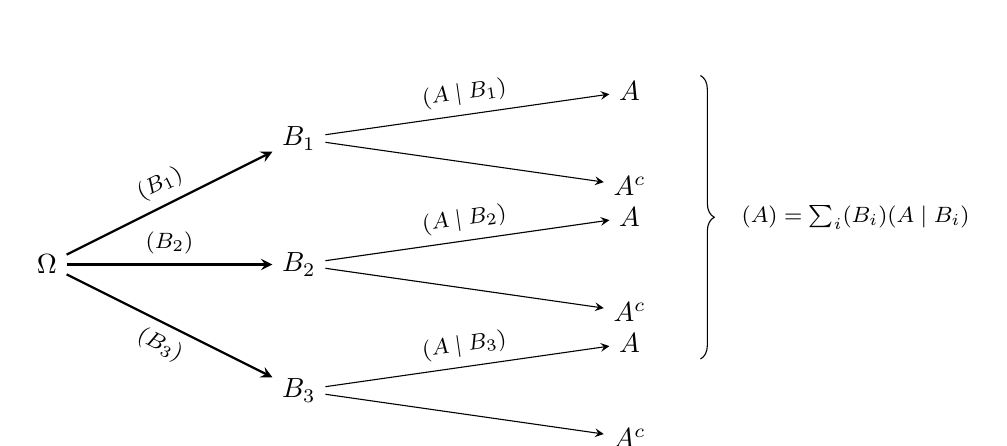
\begin{tikzpicture}[>=stealth, scale=1.0]
    \node (root) at (0,0) {$\Omega$};
    \node (b1) at (3.2,1.6) {$B_{1}$}; \node (b2) at (3.2,0.0) {$B_{2}$};
    \node (b3) at (3.2,-1.6) {$B_{3}$};
    \node (a1) at (7.4,2.2) {$A$};  \node (n1) at (7.4,1.0) {$A^{c}$};
    \node (a2) at (7.4,0.6) {$A$};  \node (n2) at (7.4,-0.6) {$A^{c}$};
    \node (a3) at (7.4,-1.0) {$A$}; \node (n3) at (7.4,-2.2) {$A^{c}$};
    \draw[->,thick] (root) -- (b1) node[midway,above,sloped] {\footnotesize $\prob(B_{1})$};
    \draw[->,thick] (root) -- (b2) node[midway,above] {\footnotesize $\prob(B_{2})$};
    \draw[->,thick] (root) -- (b3) node[midway,below,sloped] {\footnotesize $\prob(B_{3})$};
    \draw[->] (b1) -- (a1) node[midway,above,sloped] {\footnotesize $\prob(A \mid B_{1})$};
    \draw[->] (b2) -- (a2) node[midway,above,sloped] {\footnotesize $\prob(A \mid B_{2})$};
    \draw[->] (b3) -- (a3) node[midway,above,sloped] {\footnotesize $\prob(A \mid B_{3})$};
    \draw[->] (b1) -- (n1); \draw[->] (b2) -- (n2); \draw[->] (b3) -- (n3);
    \draw[decorate,decoration={brace,amplitude=5pt}] (8.3,2.4) -- (8.3,-1.2);
    \node[right] at (8.7,0.6)
      {\footnotesize $\prob(A) = \sum_{i} \prob(B_{i})\prob(A \mid B_{i})$};
  \end{tikzpicture}
\end{figure}

Reading the tree left to right gives the formule des probabilités totales: each
path to an $A$ leaf contributes the product of the probabilities along it, and
the paths are disjoint. Reading it right to left --- which branch did we come
down, given that we landed on $A$? --- is the formule de Bayes.

\begin{example}[A screening test with a small prevalence]
  On dispose d'un test pour une certaine maladie. Ce test n'est pas parfait :
  $1\%$ des individus sains sont positifs au test et $2\%$ des individus malades
  sont négatifs au test. On suppose que la maladie touche $1\%$ de la population.
  Quelle est la probabilité qu'un individu positif au test soit effectivement
  malade ?\\

  Soit $X$ l'état de l'individu et $Y$ le résultat du test. Par la formule de
  Bayes,
  \[ \prob(X = +\mid Y = +)
       = \frac{\prob(X=+)}{\prob(Y=+)}\, \prob(Y = + \mid X = +), \]
  on a $\prob(X=+) = 1\%$ et $\prob(Y=+\mid X=+) = 1 - 2\% = 98\%$. Il reste à
  appliquer la formule des probabilités totales --- for the denominator, with
  the partition $\{X=+\}, \{X=-\}$ --- pour obtenir :
  \[ \prob(Y=+) = 99\% \times 1\% + 1\% \times 98\%. \]
  Et donc
  \[ \prob(X = +\mid Y=+)
       = \frac{1\% \times 98\%}{99\% \times 1\% + 1\% \times 98\%}
       \simeq 50\%. \]
  A test that is $98\%$ and $99\%$ accurate identifies the ill barely better than
  a coin, because the prevalence and the false-positive rate are the same order
  of magnitude. The lesson is that $\prob(X \mid Y)$ and $\prob(Y \mid X)$ are
  different numbers, and that the prior is what separates them.
\end{example}

\begin{example}[Two walkers on a heptagon, as a conditioning computation]
  Two walkers move on the vertices of a heptagon, numbered $0$ to $6$. At each
  time $n$ each walker moves independently and uniformly to one of the two
  neighbouring vertices, so that with $X_{n}$ and $Y_{n}$ their positions,
  \[ \prob(X_{n+1} = X_{n} + 1 \bmod 7)
       = \prob(X_{n+1} = X_{n} - 1 \bmod 7) = \tfrac{1}{2}, \]
  and likewise for $Y_{n}$. Let $L_{n}$ be the length of the shortest path
  between the two walkers,
  \[ L_{n} = \min(X_{n} - Y_{n} \bmod 7,\ Y_{n} - X_{n} \bmod 7)
       \in \{0,1,2,3\}. \]
  Write $D_{n} = X_{n} - Y_{n} \bmod 7$, so that $L_{n} = \min(D_{n}, 7-D_{n})$.
  Each walker moves by $\pm 1$, so $D$ changes by $+2$, $0$ or $-2$ with
  probabilities $\tfrac14, \tfrac12, \tfrac14$. From $D=0$ the gap becomes $2$ or
  $5$, both at distance $2$; from $D=1$ it becomes $3$ or $6$, at distances $3$
  and $1$; from $D=2$ it becomes $4$ or $0$, at distances $3$ and $0$; from $D=3$
  it becomes $5$ or $1$, at distances $2$ and $1$. The loi of $L_{n+1}$
  therefore depends on the past only through $L_{n}$, which is the Markov
  property, and the transition probabilities
  $\prob(L_{n+1} = \ell' \mid L_{n} = \ell)$ are collected in the graph below.\\

  \begin{center}
  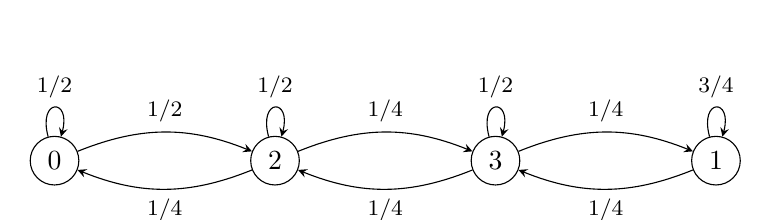
\begin{tikzpicture}[>=stealth, scale=1.0]
    \node[draw,circle] (s0) at (0,0) {$0$};   \node[draw,circle] (s2) at (2.8,0) {$2$};
    \node[draw,circle] (s3) at (5.6,0) {$3$}; \node[draw,circle] (s1) at (8.4,0) {$1$};
    \draw[->] (s0) to[bend left=22] node[above]{\footnotesize $1/2$} (s2);
    \draw[->] (s2) to[bend left=22] node[below]{\footnotesize $1/4$} (s0);
    \draw[->] (s2) to[bend left=22] node[above]{\footnotesize $1/4$} (s3);
    \draw[->] (s3) to[bend left=22] node[below]{\footnotesize $1/4$} (s2);
    \draw[->] (s3) to[bend left=22] node[above]{\footnotesize $1/4$} (s1);
    \draw[->] (s1) to[bend left=22] node[below]{\footnotesize $1/4$} (s3);
    \draw[->] (s0) to[loop above] node{\footnotesize $1/2$} (s0);
    \draw[->] (s2) to[loop above] node{\footnotesize $1/2$} (s2);
    \draw[->] (s3) to[loop above] node{\footnotesize $1/2$} (s3);
    \draw[->] (s1) to[loop above] node{\footnotesize $3/4$} (s1);
  \end{tikzpicture}
  \end{center}

  The graph is connected in both directions, so the chain is irreducible, and
  every state carries a self-loop, so it is aperiodic; the loi of $L_{n}$
  therefore converges to the stationary loi $\pi$. The balance equations ---
  each the formule des probabilités totales applied to the partition by the
  previous state ---
  \[ \pi_{0} = \tfrac12 \pi_{0} + \tfrac14 \pi_{2}, \qquad
     \pi_{1} = \tfrac34 \pi_{1} + \tfrac14 \pi_{3}, \qquad
     \pi_{2} = \tfrac12 \pi_{0} + \tfrac12 \pi_{2} + \tfrac14 \pi_{3}, \]
  gives $\pi_{1} = \pi_{2} = \pi_{3} = 2\pi_{0}$, so
  $\pi = \tfrac17 (1,2,2,2)$ after normalisation. In particular
  $\prob(L_{n} = 0) \to \tfrac17$: in the long run the two walkers occupy the
  same vertex one seventh of the time, which is what uniformity on seven
  vertices should give.
\end{example}

\subsection{Variables aléatoires}

Une \textbf{variable aléatoire} (\textit{random variable}) est une grandeur à
valeurs dans un certain ensemble ; cette valeur dépend du résultat de
l'expérience.

\begin{definition}[Variable aléatoire]
  Une \textbf{variable aléatoire} $X$ est une fonction de $\Omega$ vers un
  ensemble $E$.
\end{definition}

No measurability is required, because on a discrete $\Omega$ every subset is an
événement --- exactly the hypothesis reinstated in chapter 4. On notera
\[ \prob(X = x) = \prob(\{\omega \in \Omega : X(\omega) = x\})
                = \prob(X^{-1}(x)). \]
Comme l'univers $\Omega$ est discret, on peut supposer l'ensemble $E$ discret,
sans perte de généralité: $X$ is determined by its values on a countable set.

\begin{definition}[Loi d'une variable aléatoire]
  On appelle \textbf{loi} (\textit{distribution}) de la variable aléatoire $X$ la
  mesure de probabilité définie sur $E$ par :
  \[ \forall A \subr E, \qquad \prob_{X}(A) = \prob(X \in A). \]
\end{definition}

Comme toute mesure de probabilité discrète, la loi est entièrement caractérisée
par ses valeurs prises sur les singletons, soit $\prob_{X}(x) = \prob(X = x)$.
Chapter 4 will identify $\prob_{X}$ as the mesure image of $\prob$ under $X$, an
object chapter 2 defines.

\begin{notation}
  Several letters are reused deliberately --- $\mathcal{P}$, $\mathcal{B}$ and
  three more --- and chapter 2 sets those collisions out in full; the argument
  in the parentheses disambiguates in every case.
\end{notation}

\textbf{Lois discrètes.} Nous donnons ici quelques lois discrètes usuelles ---
the five the course uses, tabulated below. Their espérances, variances and
fonctions génératrices are computed in the three subsections that follow.

\begin{center}
  \begin{tabular}{lllll}
    \toprule
    Nom & Paramètre(s) & Notation & Support & $\prob(X = k)$ \\
    \midrule
    Bernoulli & $p \in [0,1]$ & $\mathcal{B}(p)$ & $\{0,1\}$ & $p$ if $k=1$, $1-p$ if $k=0$ \\
    Binomiale & $n \in \mathbb{N},\ p \in [0,1]$ & $\mathcal{B}(n,p)$ & $\{0,\dots,n\}$ & $\binom{n}{k} p^{k}(1-p)^{n-k}$ \\
    Poisson & $\lambda > 0$ & $\mathcal{P}(\lambda)$ & $\mathbb{N}$ & $e^{-\lambda} \lambda^{k}/k!$ \\
    Géométrique & $p \in\, ]0,1]$ & $\mathcal{G}(p)$ & $\mathbb{N}^{*}$ & $(1-p)^{k-1} p$ \\
    Uniforme & $n \in \mathbb{N}^{*}$ & $\mathcal{U}(1,\dots,n)$ & $\{1,\dots,n\}$ & $1/n$ \\
    \bottomrule
  \end{tabular}
\end{center}

The binomial counts the successes among $n$ independent Bernoulli trials of the
same parameter; the geometric counts the trials up to and including the first
success, so its support starts at $1$.

\begin{figure}[h!]
  \centering
  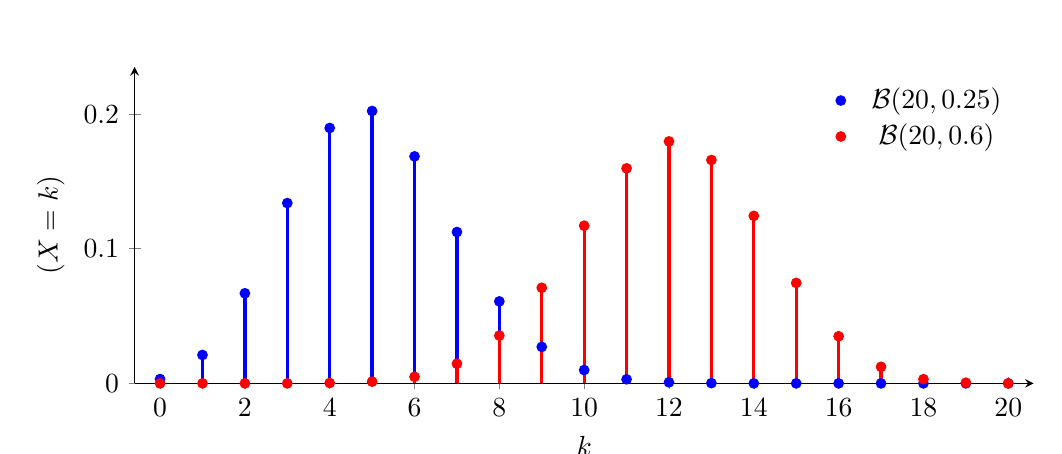
\begin{tikzpicture}
    \begin{axis}[width=13cm, height=5.6cm, axis lines=left,
      xlabel={$k$}, ylabel={$\prob(X = k)$},
      xmin=-0.6, xmax=20.6, ymin=0, ymax=0.235, xtick={0,2,4,6,8,10,12,14,16,18,20},
      legend style={at={(0.98,0.97)}, anchor=north east, draw=none}]
      \addplot[ycomb, very thick, mark=*, mark size=1.3pt, blue] coordinates {
        (0,0.0032) (1,0.0211) (2,0.0669) (3,0.1339) (4,0.1897) (5,0.2023)
        (6,0.1686) (7,0.1124) (8,0.0609) (9,0.0271) (10,0.0099) (11,0.0030)
        (12,0.0008) (13,0.0002) (14,0) (15,0) (16,0) (17,0) (18,0) (19,0) (20,0) };
      \addlegendentry{$\mathcal{B}(20, 0.25)$}
      \addplot[ycomb, very thick, mark=*, mark size=1.3pt, red] coordinates {
        (0,0) (1,0) (2,0) (3,0) (4,0.0003) (5,0.0013) (6,0.0049) (7,0.0146)
        (8,0.0355) (9,0.0710) (10,0.1171) (11,0.1597) (12,0.1797) (13,0.1659)
        (14,0.1244) (15,0.0746) (16,0.0350) (17,0.0123) (18,0.0031) (19,0.0005) (20,0) };
      \addlegendentry{$\mathcal{B}(20, 0.6)$}
    \end{axis}
  \end{tikzpicture}
\end{figure}

Both binomials above have $n = 20$. The mass concentrates around $np$ --- $5$ and
$12$ respectively --- and the spread is governed by $np(1-p)$, which is largest
at $p = \tfrac12$; the right-hand loi, being nearer the symmetric case,
is the wider of the two.

\begin{figure}[h!]
  \centering
  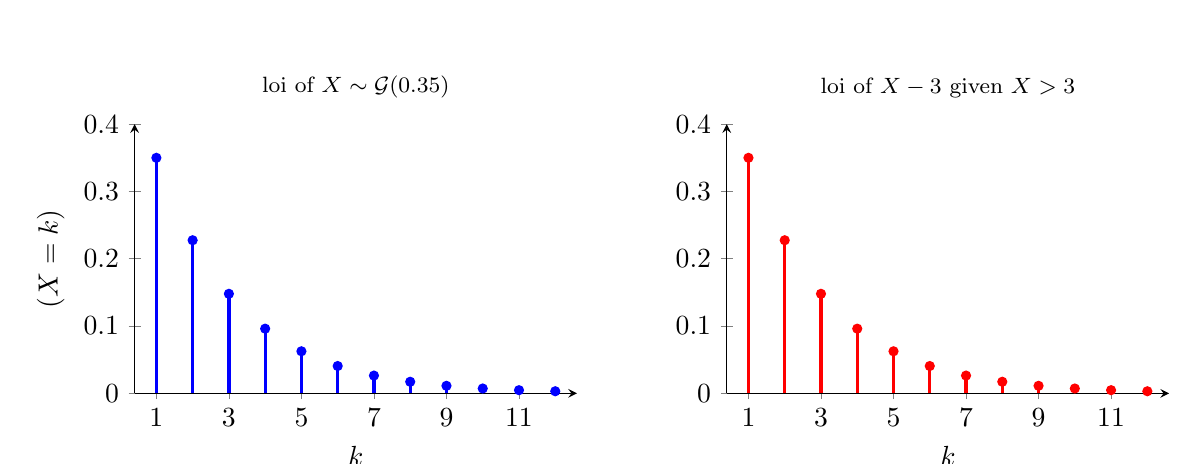
\begin{tikzpicture}
    \begin{axis}[name=left, width=7.2cm, height=5.0cm, axis lines=left,
      xlabel={$k$}, ylabel={$\prob(X = k)$},
      title={\footnotesize loi of $X \sim \mathcal{G}(0.35)$},
      xmin=0.4, xmax=12.6, ymin=0, ymax=0.40, xtick={1,3,5,7,9,11}]
      \addplot[ycomb, very thick, mark=*, mark size=1.2pt, blue] coordinates {
        (1,0.3500) (2,0.2275) (3,0.1479) (4,0.0961) (5,0.0625) (6,0.0406)
        (7,0.0264) (8,0.0172) (9,0.0112) (10,0.0072) (11,0.0047) (12,0.0031) };
    \end{axis}
    \begin{axis}[at={(left.right of origin)}, anchor=left of origin, xshift=1.9cm,
      width=7.2cm, height=5.0cm, axis lines=left, xlabel={$k$},
      title={\footnotesize loi of $X - 3$ given $X > 3$},
      xmin=0.4, xmax=12.6, ymin=0, ymax=0.40, xtick={1,3,5,7,9,11}]
      \addplot[ycomb, very thick, mark=*, mark size=1.2pt, red] coordinates {
        (1,0.3500) (2,0.2275) (3,0.1479) (4,0.0961) (5,0.0625) (6,0.0406)
        (7,0.0264) (8,0.0172) (9,0.0112) (10,0.0072) (11,0.0047) (12,0.0031) };
    \end{axis}
  \end{tikzpicture}
\end{figure}

The two panels are the same picture: this is the \textbf{absence de mémoire}
(\textit{memorylessness}) of the loi géométrique. Since
$\prob(X > k) = (1-p)^{k}$ on the support $\mathbb{N}^{*}$,
\[ \prob(X > n + k \mid X > n)
     = \frac{(1-p)^{n+k}}{(1-p)^{n}} = (1-p)^{k} = \prob(X > k). \]
Three failed trials leave the number of further trials distributed exactly as at
the start. The geometric is the only discrete loi with this property; the loi
exponentielle of chapter 4 is its continuous counterpart.

\subsection{Loi conditionnelle}

Soit $X$ une variable aléatoire à valeurs dans $E$.

\begin{definition}[Loi conditionnelle]
  Soit $A$ un événement tel que $\prob(A) > 0$. On appelle \textbf{loi
  conditionnelle} (\textit{conditional distribution}) de $X$ sachant $A$ la
  mesure de probabilité $\prob_{X \mid A}$ définie sur $E$ par :
  \[ \forall B \subr E, \qquad \prob_{X \mid A}(B) = \prob(X \in B \mid A). \]
\end{definition}

C'est la mesure image de la probabilité conditionnelle $\prob(\cdot \mid A)$ par
$X$. As before $\prob(A) > 0$ is what makes the definition legitimate; chapter 5
removes it, at the cost of defining the loi conditionnelle only up to a
négligeable set.

\begin{example}[Restricting a uniform die]
  Soit $X$ une variable aléatoire de loi uniforme sur $\{1,\dots,6\}$. La loi
  conditionnelle de $X$ sachant $X \le 3$ est une loi uniforme sur $\{1,2,3\}$.
  Each surviving value keeps the weight $\tfrac16$, and renormalising by
  $\prob(X \le 3) = \tfrac12$ turns it into $\tfrac13$. Conditioning a loi
  uniforme on a subset of its support gives the loi uniforme on that subset ---
  only because the weights were equal to begin with.
\end{example}

\subsection{Loi jointe, lois marginales}

Soit $X$ et $Y$ deux variables aléatoires à valeurs respectives dans $E$ et $F$.
Le couple $(X,Y)$ définit une variable aléatoire sur $E \times F$.

\begin{definition}[Loi jointe, lois marginales]
  La loi du couple $(X,Y)$, notée $\prob_{X,Y}$, est appelée la \textbf{loi
  jointe} (\textit{joint distribution}) de $X$ et $Y$. Les lois $\prob_{X}$ et
  $\prob_{Y}$ sont les \textbf{lois marginales} (\textit{marginal distributions})
  du couple.
\end{definition}

La loi jointe est une mesure de probabilité discrète, entièrement caractérisée
par ses valeurs sur les singletons :
\[ \forall x \in E,\ \forall y \in F, \qquad
   \prob_{X,Y}(\{x\} \times \{y\}) = \prob(X = x, Y = y), \]
et les lois marginales s'en déduisent, by summing out the other coordinate :
\[ \prob_{X}(x) = \sum_{y \in F} \prob(X = x, Y = y), \qquad
   \prob_{Y}(y) = \sum_{x \in E} \prob(X = x, Y = y). \]
The converse fails: the lois marginales do not determine the loi jointe, which
is what makes the next definition non-trivial.

\begin{definition}[Indépendance de deux variables aléatoires]
  Deux variables aléatoires $X$ et $Y$ sont dites \textbf{indépendantes} si pour
  tous $A \subr E$ et $B \subr F$, les événements $\{X \in A\}$ et
  $\{Y \in B\}$ sont indépendants, soit :
  \[ \prob(X \in A, Y \in B) = \prob(X \in A)\,\prob(Y \in B). \]
\end{definition}

\begin{prop}
  Deux variables aléatoires $X$ et $Y$ sont indépendantes si et seulement si
  \[ \forall x \in E,\ \forall y \in F, \qquad
     \prob(X = x, Y = y) = \prob(X = x)\prob(Y = y). \]
\end{prop}

Though indépendance quantifies over all pairs of subsets, la loi du couple étant
une loi discrète, il suffit de vérifier cette propriété sur les singletons;
summing recovers the general case. De façon équivalente,
les variables aléatoires $X$ et $Y$ sont indépendantes si et seulement si pour
tout $x \in E$ tel que $\prob(X=x) > 0$, la loi conditionnelle de $Y$ sachant
$X = x$ est la loi de $Y$.

\begin{prop}
  Si les variables aléatoires $X$ et $Y$ sont indépendantes, alors les
  variables aléatoires $\phi(X)$ et $\psi(Y)$ sont indépendantes, quelles que
  soient les fonctions $\phi$ et $\psi$.
\end{prop}

No hypothesis at all is needed on $\phi$ and $\psi$; in chapter 4 they must be
mesurables, which is the only change.

\begin{example}[Thinning a Poisson count by a fair coin]
  Une tortue donne naissance à $N$ bébés. On suppose que $N$ suit une loi de
  Poisson $\mathcal{P}(\lambda)$. Chaque bébé a une chance sur deux
  ($\tfrac{1}{2}$) d'être une femelle, independently of the others. On note $F$
  le nombre de bébés femelles.\\

  Conditionally on $N = n$, the variable $F$ counts the successes among $n$
  independent fair trials: sa loi conditionnelle est une loi binomiale
  $\mathcal{B}(n, \tfrac12)$. La loi jointe du couple est :
  \[ \forall 0 \le k \le n, \qquad
     \prob(N = n, F = k) = \prob(N=n)\prob(F = k \mid N = n)
       = e^{-\lambda} \frac{\lambda^{n}}{n!} \binom{n}{k} \frac{1}{2^{n}}. \]
  Summing over $n \ge k$, and substituting $m = n-k$,
  \[ \prob(F = k) = e^{-\lambda} \left(\frac{\lambda}{2}\right)^{k}
       \frac{1}{k!} \sum_{m \ge 0} \left(\frac{\lambda}{2}\right)^{m}
       \frac{1}{m!}
     = e^{-\lambda/2} \left(\frac{\lambda}{2}\right)^{k} \frac{1}{k!}, \]
  so $F$ follows the loi de Poisson $\mathcal{P}(\lambda/2)$. Thinning a
  Poisson count keeps it Poisson and halves the parameter.\\

  Les variables ne sont \emph{pas} indépendantes car la loi de $F$ sachant
  $N = 0$ est un Dirac en $0$, qui est différente de la loi de $F$. Having the
  same family of lois is no substitute for checking the product identity.
\end{example}

\subsection{Espérance}

Soit $X$ une variable aléatoire à valeurs réelles.

\begin{definition}[Espérance]
  L'\textbf{espérance} (\textit{expectation}) de la variable aléatoire $X$ est la
  valeur, éventuellement infinie,
  \[ \expec(X) = \sum_{\omega \in \Omega} X(\omega)\prob(\omega), \]
  pourvu que $X$ soit positive ou que $\expec(|X|) < \infty$.
\end{definition}

The proviso is the whole hypothesis. A sum over a countable index set is
order-independent only when its terms are positive or the sum is absolutely
convergent; without one of the two, $\expec(X)$ is not even well-defined. Every
manipulation below rests on it.

\begin{prop}
  L'espérance de la variable aléatoire $X$ dépend uniquement de sa loi :
  \[ \expec(X) = \sum_{x \in E} x \, \prob(X = x), \]
  pourvu que $X$ soit positive ou que $\expec(|X|) < \infty$.
\end{prop}

Une variable aléatoire d'espérance nulle est dite \textbf{centrée}
(\textit{centred}).

\begin{example}[The espérance of an indicator is a probability]
  Soit $A \subr \Omega$ un événement. Alors la variable aléatoire
  $X = \indic_{A}$ suit une loi de Bernoulli $\mathcal{B}(\prob(A))$, de sorte
  que
  \[ \expec(\indic_{A}) = \prob(A). \]
  This one line is the bridge between counting and probability, and it is the
  engine of the linearity arguments below.
\end{example}

\begin{example}[Espérances des cinq lois]
  L'espérance d'une variable aléatoire $X \sim \mathcal{B}(p)$ est
  $\expec(X) = \prob(X=1) = p$.\\

  L'espérance d'une variable aléatoire $X \sim \mathcal{P}(\lambda)$ est
  \[ \expec(X) = \sum_{k \ge 0} k\, e^{-\lambda} \frac{\lambda^{k}}{k!}
       = \lambda e^{-\lambda} \sum_{k \ge 1} \frac{\lambda^{k-1}}{(k-1)!}
       = \lambda. \]
  L'espérance d'une variable aléatoire $X \sim \mathcal{U}(1,\dots,n)$ est
  $\expec(X) = \frac{1+2+\dots+n}{n} = \frac{n+1}{2}$.\\

  For $X \sim \mathcal{B}(n,p)$, writing $X = \sum_{i=1}^{n} X_{i}$ with the
  $X_{i}$ independent $\mathcal{B}(p)$ and using linearity below,
  $\expec(X) = np$. For $X \sim \mathcal{G}(p)$,
  \[ \expec(X) = \sum_{k \ge 1} k(1-p)^{k-1} p
       = p \cdot \frac{1}{p^{2}} = \frac{1}{p}, \]
  using $\sum_{k \ge 1} k q^{k-1} = (1-q)^{-2}$ for $|q| < 1$.
\end{example}

\begin{theorem}[Transfert (\textit{transfer theorem})]
  Soit $X$ une variable aléatoire à valeurs dans $E$. Pour toute fonction
  $\phi : E \to \reals$,
  \[ \expec(\phi(X)) = \sum_{x \in E} \phi(x) \prob(X = x), \]
  pourvu que $\phi$ soit positive ou que $\expec(|\phi(X)|) < \infty$.
\end{theorem}

To compute the espérance of $\phi(X)$ one never needs $\Omega$: the loi of $X$
suffices, which is why a variable can be described by its loi alone. The
hypothesis is again positivity \emph{or} integrability, and it bears on
$\phi(X)$, not on $X$: $X$ may be integrable while $X^{2}$ is not.

\begin{corollary}[Linéarité]
  Soit $X$, $Y$ deux variables aléatoires réelles d'espérances finies. Alors,
  \[ \forall \alpha \in \reals, \quad \expec(\alpha X) = \alpha \expec(X),
     \qquad \text{and} \qquad
     \expec(X+Y) = \expec(X) + \expec(Y). \]
\end{corollary}

\begin{remark}
  Linearity requires \emph{finite} espérances and nothing else: $X$ and $Y$ need
  not be independent, so $\expec(X+Y) = \expec(X) + \expec(Y)$ holds for
  arbitrarily dependent variables. On raisonne en appliquant le théorème de
  transfert au couple $(X,Y)$, the absolute convergence coming from the
  finiteness hypothesis. Contrast the product rule below, which does need
  indépendance, and the variance of a sum, which does not split without it.
\end{remark}

\begin{prop}[Espérance d'une série]
  Pour toute suite de variables aléatoires réelles $(X_{n})_{n \ge 1}$,
  \[ \expec\left( \sum_{n \ge 1} X_{n} \right) = \sum_{n \ge 1} \expec(X_{n}) \]
  dès que les variables aléatoires $X_{n}$ sont positives pour tout $n \ge 1$ ou
  que $\sum_{n \ge 1} \expec(|X_{n}|) < \infty$.
\end{prop}

This is linearity extended to a countable sum, and the discrete form of the
convergence monotone and convergence dominée theorems of chapter 3. The second
hypothesis bounds the \emph{sum} of the $\expec(|X_{n}|)$, not each term
separately.

\begin{prop}
  Pour toutes variables aléatoires réelles $X$, $Y$ indépendantes d'espérances
  finies,
  \[ \expec(XY) = \expec(X)\expec(Y). \]
\end{prop}

Indépendance is essential; finiteness of $\expec(X)$ and $\expec(Y)$ then gives
$\expec(|XY|) = \expec(|X|)\expec(|Y|) < \infty$, so $XY$ is automatically
integrable. The converse is false: $\expec(XY) = \expec(X)\expec(Y)$ says only
that $X$ and $Y$ are décorrélées, which is weaker than indépendance.

\begin{example}[Fixed points of a random ordering, by indicators and linearity]
  One object here is borrowed from chapter 4 and one is not: the variables to be
  sorted are continuous, and so outside this chapter, but the permutation that
  sorts them takes finitely many values, so it is a discrete variable aléatoire
  and the computation below lives entirely in the present setting.\\

  Let $X_{1}, \dots, X_{n}$ be \textbf{indépendantes et identiquement
  distribuées} (\textit{independent and identically distributed}) real variables
  aléatoires, abbreviated i.i.d.\ from here on, whose common
  loi has a densité --- an object chapter 4 builds, quoted here only for
  the one fact that $\prob(X_{i} = X_{j}) = 0$ for $i \ne j$;
  by the borne de l'union, $\prob(\exists i \ne j,\ X_{i} = X_{j}) = 0$. There
  is therefore presque sûrement a unique permutation $\sigma$ of
  $\{1,\dots,n\}$ that sorts them,
  $X_{\sigma(1)} < \dots < X_{\sigma(n)}$, and $\sigma$ is a variable aléatoire
  with values in the set of permutations.\\

  Because the $X_{i}$ are i.i.d., for every fixed permutation $s$,
  \[ \prob(\sigma = s) = \prob(X_{s(1)} < \dots < X_{s(n)})
                       = \prob(X_{1} < \dots < X_{n}), \]
  a quantity that does not depend on $s$, so $\sigma$ is uniform on the $n!$
  permutations. In particular $\prob(\sigma(i) = j) = \tfrac1n$ for all $i,j$.\\

  How many fixed points does $\sigma$ have on average? Write the count as a sum
  of indicators and use linearity:
  \[ \expec\left( \sum_{i=1}^{n} \indic_{\{\sigma(i) = i\}} \right)
       = \sum_{i=1}^{n} \expec(\indic_{\{\sigma(i)=i\}})
       = \sum_{i=1}^{n} \prob(\sigma(i) = i)
       = n \cdot \frac{1}{n} = 1. \]
  The answer is $1$ for every $n$, and the événements $\{\sigma(i)=i\}$ are
  heavily dependent --- knowing $n-1$ of them determines the last --- which
  linearity does not care about. The method is the one to keep for any counting
  espérance: decompose into indicators, take espérances termwise, read each term
  as a probability.
\end{example}

\subsection{Variance, covariance}

Soit $X$ une variable aléatoire réelle d'espérance finie.

\begin{definition}[Variance]
  La \textbf{variance} de la variable aléatoire $X$ est la valeur, éventuellement
  infinie :
  \[ \Var(X) = \expec\big( (X - \expec(X))^{2} \big). \]
\end{definition}

Par linéarité de l'espérance, on obtient l'expression équivalente :
\[ \Var(X) = \expec(X^{2}) - \expec(X)^{2}, \]
which is the one to compute with; it comes from expanding the square.

\begin{prop}
  On a $\Var(X) \ge 0$ avec $\Var(X) = 0$ si et seulement si $X = \expec(X)$ p.s.
\end{prop}

The abbreviation \textit{p.s.} means \textbf{presque sûrement} (\textit{almost
surely}), c'est-à-dire avec probabilité $1$; it is kept in its French form. Here it says
$X(\omega) = \expec(X)$ for every $\omega$ with $\prob(\omega) > 0$: the
values of $X$ on the null part of $\Omega$ are unconstrained, which is why the
conclusion is not $X = \expec(X)$ everywhere.\\

Par linéarité de l'espérance, on a :
\[ \forall \alpha \in \reals, \qquad \Var(\alpha X) = \alpha^{2} \Var(X). \]
The variance scales quadratically: the square is the entire content of the
rule, and the reason the écart type $\sqrt{\Var(X)}$, not the variance, is the
quantity with the same units as $X$. In particular $\Var(-X) = \Var(X)$, the case $\alpha = -1$. Separately,
$\Var(X + c) = \Var(X)$ for a constant $c$, which does not follow from the
scaling rule but straight from the definition: adding $c$ moves $X$ and
$\expec(X)$ by the same amount, so $X + c - \expec(X+c) = X - \expec(X)$.\\

On considère maintenant $X$ et $Y$ deux variables aléatoires de variances finies.

\begin{definition}[Covariance]
  La \textbf{covariance} entre les variables aléatoires $X$ et $Y$ est la
  valeur :
  \[ \Cov(X,Y) = \expec\big( (X - \expec(X))(Y - \expec(Y)) \big). \]
\end{definition}

Finiteness of the two variances is what makes this well-defined: on en déduit
que $\expec(X^{2}) < \infty$ et $\expec(Y^{2}) < \infty$. En utilisant le fait
que $|XY| \le \tfrac{1}{2}(X^{2} + Y^{2})$, on obtient que $XY$ est d'espérance
finie. Par linéarité de l'espérance --- after expanding the product --- on
obtient alors :
\[ \Cov(X,Y) = \expec(XY) - \expec(X)\expec(Y). \]
On note que $\Cov(X,Y) = 0$ dès que $X$ et $Y$ sont indépendantes. La
réciproque est fausse.\\

La covariance vérifie les propriétés suivantes :
\begin{itemize}
  \item $\Cov(X,X) = \Var(X)$;
  \item $\Cov(X,Y) = \Cov(Y,X)$;
  \item $\Cov(\alpha X, Y) = \alpha \Cov(X,Y)$ pour tout $\alpha \in \reals$;
  \item $\Cov(X, Y+Z) = \Cov(X,Y) + \Cov(X,Z)$ pour toutes variables $X,Y,Z$ de
    variances finies.
\end{itemize}
En particulier, la covariance est une forme bilinéaire symétrique.

\begin{remark}
  La covariance n'est \emph{pas} \textbf{définie positive} (\textit{positive
  definite}) car $\Var(X) = 0$ implique uniquement que $X$ est p.s.\ constante,
  not zero. La covariance n'est définie positive que si l'on se restreint aux
  variables aléatoires centrées --- identifying two that are p.s.\ equal. Elle
  définit alors un produit scalaire.
  That structure is the right way to see the next two results: the variance of a
  sum is an expansion of $\|X+Y\|^{2}$, and Cauchy--Schwartz is Cauchy--Schwartz.
\end{remark}

\begin{prop}
  On a pour toutes variables aléatoires $X$ et $Y$ de variances finies :
  \[ \Var(X+Y) = \Var(X) + 2\Cov(X,Y) + \Var(Y). \]
\end{prop}

\begin{corollary}
  Si les variables aléatoires $X$ et $Y$ sont indépendantes et de variances
  finies, alors $\Cov(X,Y) = 0$ et
  \[ \Var(X+Y) = \Var(X) + \Var(Y). \]
\end{corollary}

The cross term is the only place indépendance enters. Espérances add for any
pair of integrable variables; variances add only when the covariance vanishes,
and vanishing covariance is weaker than indépendance, so the corollary is
genuinely weaker than the proposition. With the scaling rule, for independent
$X, Y$ and reals $a, b$,
\[ \Var(aX + bY) = a^{2}\Var(X) + b^{2}\Var(Y), \]
the squares again.

\begin{prop}[Inégalité de Cauchy-Schwartz (\textit{Cauchy--Schwartz inequality})]
  On a pour toutes variables aléatoires $X$ et $Y$ de variances finies :
  \[ |\Cov(X,Y)| \le \sqrt{\Var(X)\Var(Y)}. \]
\end{prop}

The name is spelled \emph{Cauchy--Schwartz} throughout. On peut supposer les
variables aléatoires $X$ et $Y$ centrées, quitte à considérer les variables
$X - \expec(X)$ et $Y - \expec(Y)$, which changes neither side. Le résultat est
alors une conséquence du fait que la covariance définit un produit scalaire: the
inequality is Cauchy--Schwartz for the inner product of the remark above.

\begin{definition}[Coefficient de corrélation]
  Le \textbf{coefficient de corrélation} (\textit{correlation coefficient}) entre
  deux variables aléatoires $X$ et $Y$ de variances finies et non nulles est la
  valeur :
  \[ \rho(X,Y) = \frac{\Cov(X,Y)}{\sqrt{\Var(X)\Var(Y)}}. \]
\end{definition}

The variances must be non-zero for the quotient to exist --- a p.s.\ constant
variable has no correlation with anything. Au vu de l'inégalité de
Cauchy-Schwartz, on a $\rho(X,Y) \in [-1,1]$, avec $|\rho(X,Y)| = 1$ si et
seulement si $X$ et $Y$ sont linéairement dépendantes, à savoir
$\rho(X,Y) = 1$ si et seulement si $Y = aX+b$ avec $a > 0$, et
$\rho(X,Y) = -1$ si et seulement si $Y = aX+b$ avec $a < 0$. Lorsque
$\rho(X,Y) = 0$, on dit que les variables sont \textbf{décorrélées}
(\textit{uncorrelated}). The coefficient is
the cosine of the ``angle'' between the two variables centrées.

\begin{figure}[h!]
  \centering
  \begin{tikzpicture}
    \begin{axis}[name=p1, scale only axis, width=4.6cm, height=4.6cm,
      axis lines=middle,
      title={\footnotesize $\rho = -1$}, xtick=\empty, ytick=\empty,
      xmin=-1.4, xmax=1.4, ymin=-1.4, ymax=1.4]
      \addplot[only marks, mark=*, mark size=1.4pt, blue] coordinates {
        (-1.2,1.2) (-0.9,0.9) (-0.6,0.6) (-0.3,0.3) (0,0)
        (0.3,-0.3) (0.6,-0.6) (0.9,-0.9) (1.2,-1.2) };
    \end{axis}
    \begin{axis}[at={(p1.right of origin)}, anchor=left of origin, xshift=1.5cm,
      name=p2, scale only axis, width=4.6cm, height=4.6cm, axis lines=middle,
      title={\footnotesize $\rho = 0$, yet dependent}, xtick=\empty, ytick=\empty,
      xmin=-1.4, xmax=1.4, ymin=-1.4, ymax=1.4]
      \addplot[only marks, mark=*, mark size=1.4pt, red] coordinates {
        (1.0,0) (0.87,0.5) (0.5,0.87) (0,1.0) (-0.5,0.87) (-0.87,0.5) (-1.0,0)
        (-0.87,-0.5) (-0.5,-0.87) (0,-1.0) (0.5,-0.87) (0.87,-0.5) };
    \end{axis}
    \begin{axis}[at={(p2.right of origin)}, anchor=left of origin, xshift=1.5cm,
      scale only axis, width=4.6cm, height=4.6cm, axis lines=middle,
      title={\footnotesize $\rho = +1$}, xtick=\empty, ytick=\empty,
      xmin=-1.4, xmax=1.4, ymin=-1.4, ymax=1.4]
      \addplot[only marks, mark=*, mark size=1.4pt, blue] coordinates {
        (-1.2,-1.2) (-0.9,-0.9) (-0.6,-0.6) (-0.3,-0.3) (0,0)
        (0.3,0.3) (0.6,0.6) (0.9,0.9) (1.2,1.2) };
    \end{axis}
  \end{tikzpicture}
\end{figure}

The outer panels are the extreme cases: all the mass on a line, $\rho = \pm 1$ by
the slope's sign. The middle panel is the one to remember --- the mass is uniform
on a circle, so by symmetry $\expec(X) = \expec(Y) = \expec(XY) = 0$ and the
coordinates are décorrélées, yet $X$ determines $Y$ up to a sign. Correlation
measures only the \emph{linear} part of a dependence, so $\rho = 0$ is strictly
weaker than indépendance.

\begin{example}[Uncorrelated but not independent]
  Soit $X$ une variable aléatoire de loi uniforme sur $\{0,1\}$ et $Z$ une
  variable aléatoire de loi uniforme sur $\{-1,+1\}$ indépendante de $X$. On note
  $Y = XZ$. Since $\expec(Z) = 0$ and $Z$ is independent of $X$ and
  of $X^{2}$,
  \[ \expec(Y) = \expec(XZ) = \expec(X)\expec(Z) = 0, \qquad
     \expec(XY) = \expec(X^{2}Z) = \expec(X^{2})\expec(Z) = 0, \]
  so $\Cov(X,Y) = \expec(XY) - \expec(X)\expec(Y) = 0$ and the variables are
  décorrélées. Par contre, $\prob(X=0, Y=1) = 0$ tandis que
  $\prob(X=0) = \tfrac12$ et $\prob(Y=1) = \tfrac14$, donc les variables ne sont
  pas indépendantes: the product identity fails on a single pair of singletons.
  One pair suffices to break indépendance.
\end{example}

\begin{example}[Variances des cinq lois]
  For $X \sim \mathcal{B}(p)$, $X^{2} = X$ so
  $\Var(X) = p - p^{2} = p(1-p)$.\\

  For $X \sim \mathcal{B}(n,p)$, write $X$ as a sum of $n$ independent Bernoulli
  variables; the covariances vanish and the variances add, giving
  $\Var(X) = np(1-p)$. This is the corollary above doing real work: the
  summands are not identically zero, but their pairwise covariances are.\\

  For $X \sim \mathcal{P}(\lambda)$, $\expec(X(X-1)) = \lambda^{2}$, so
  $\expec(X^{2}) = \lambda^{2} + \lambda$ and $\Var(X) = \lambda$: the loi de
  Poisson has equal mean and variance. For $X \sim \mathcal{G}(p)$,
  $\Var(X) = \frac{1-p}{p^{2}}$, and for $X \sim \mathcal{U}(1,\dots,n)$,
  $\Var(X) = \frac{n^{2}-1}{12}$.
\end{example}

\subsection{Fonction génératrice}

La fonction génératrice d'une variable aléatoire à valeurs entières positives
permet de caractériser la loi et d'en calculer les moments.

\begin{definition}[Fonction génératrice]
  La \textbf{fonction génératrice} (\textit{generating function}) d'une variable
  aléatoire $X$ à valeurs dans $\mathbb{N}$ est la fonction $G_{X}$ définie
  par :
  \[ \forall t \in [-1,1], \qquad
     G_{X}(t) = \expec(t^{X}) = \sum_{k \ge 0} \prob(X = k)\, t^{k}. \]
\end{definition}

The hypothesis that $X$ takes values in $\mathbb{N}$ is what the construction
needs: $t^{X}$ must be a power series in $t$. Il s'agit d'une série entière de
rayon de convergence supérieur ou égal à $1$ --- the coefficients sum to $1$ ---
et $G_{X}$ est donc une fonction continue sur $[-1,1]$ et $C^{\infty}$ sur
$]-1,1[$. The endpoints are the delicate ones, and the one-sided derivative at
$1$ below is where the moments live.

\begin{prop}
  On a $\prob(X = 0) = G_{X}(0)$ et pour tout $k \ge 1$,
  \[ \prob(X = k) = \frac{1}{k!} \frac{d^{k} G_{X}}{dt^{k}}(0). \]
\end{prop}

Ce résultat montre que la fonction génératrice caractérise la loi: two
$\mathbb{N}$-valued variables with the same fonction génératrice have the same
loi. That is the first of its two uses.\\

The second is moments. La fonction génératrice a toujours une dérivée à gauche
en $1$, éventuellement infinie, et on a :
\[ \expec(X) = G_{X}'(1^{-}). \]
More generally the $k$-th \textbf{factorial moment} is read off the $k$-th
left derivative, when that derivative is finite:
\[ \expec\big( X(X-1)\cdots(X-k+1) \big)
     = \frac{d^{k} G_{X}}{dt^{k}}(1^{-}). \]
The derivative is a \emph{left} derivative at $1$, since $G_{X}$ is only defined
on $[-1,1]$, and it may be infinite --- exactly when $X$ has no moment of that
order. From the factorial moments the ordinary ones follow:
$\expec(X^{2}) = G_{X}''(1^{-}) + G_{X}'(1^{-})$, and then
$\Var(X) = G_{X}''(1^{-}) + G_{X}'(1^{-}) - G_{X}'(1^{-})^{2}$.

\begin{prop}
  Soit $X$, $Y$ deux variables aléatoires indépendantes à valeurs dans
  $\mathbb{N}$. Alors,
  \[ G_{X+Y} = G_{X} G_{Y}. \]
\end{prop}

The proof is one line --- $\expec(t^{X+Y}) = \expec(t^{X})\expec(t^{Y})$ by
indépendance --- and the consequence is that a convolution of lois becomes a
product of functions. Indépendance is indispensable; without it the espérance of
the product does not factor.

\begin{remark}
  These two properties are exactly what makes the fonction caractéristique
  $\varphi_{X}$ of chapter 6 worth building: $\varphi_{X}(t) = \expec(e^{itX})$
  characterises the loi of \emph{any} real variable aléatoire, its
  derivatives at $0$ give the moments, and $\varphi_{X+Y} = \varphi_{X}\varphi_{Y}$ for
  independent summands. The fonction génératrice is the same idea restricted to
  $\mathbb{N}$-valued variables, with $t$ for $e^{it}$: cheaper, real-valued, and
  enough whenever the variable counts something.
\end{remark}

\begin{example}[Fonctions génératrices des cinq lois]
  La fonction génératrice d'une variable aléatoire $X \sim \mathcal{B}(p)$ est
  $G_{X}(t) = 1 - p + pt$. For
  $X \sim \mathcal{B}(n,p)$, the binomial is a sum of $n$ independent Bernoulli
  variables, so the product rule gives $G_{X}(t) = (1-p+pt)^{n}$ at once.\\

  La fonction génératrice d'une variable aléatoire $X \sim \mathcal{P}(\lambda)$
  est
  \[ G_{X}(t) = \sum_{k \ge 0} e^{-\lambda} \frac{\lambda^{k}}{k!} t^{k}
       = e^{-\lambda} e^{\lambda t} = e^{\lambda(t-1)}. \]
  For $X \sim \mathcal{G}(p)$, summing the geometric series,
  $G_{X}(t) = \frac{pt}{1 - (1-p)t}$, which is finite for every
  $t \in [-1,1]$ when $p \in\, ]0,1]$. For $X \sim \mathcal{U}(1,\dots,n)$,
  $G_{X}(t) = \frac{t}{n}\frac{1-t^{n}}{1-t}$ for $t \ne 1$, and $G_{X}(1) = 1$.
\end{example}

\begin{example}[The sum of two independent Poisson counts]
  Soit $X$, $Y$ des variables aléatoires indépendantes suivant des lois de
  Poisson $\mathcal{P}(\alpha)$ et $\mathcal{P}(\beta)$. Then
  \[ G_{X+Y}(t) = G_{X}(t)G_{Y}(t)
       = e^{\alpha(t-1)} e^{\beta(t-1)} = e^{(\alpha+\beta)(t-1)}, \]
  which is the fonction génératrice of $\mathcal{P}(\alpha+\beta)$. Since the
  fonction génératrice characterises the loi, $X + Y \sim
  \mathcal{P}(\alpha+\beta)$. Computing the same convolution directly means
  summing $\sum_{j} \prob(X=j)\prob(Y=k-j)$ and recognising a binomial
  expansion; the fonction génératrice makes it a product of exponentials.
\end{example}

\begin{center}
  \begin{tabular}{lcccc}
    \toprule
    Loi & Support & $\expec(X)$ & $\Var(X)$ & $G_{X}(t)$ \\
    \midrule
    $\mathcal{B}(p)$ & $\{0,1\}$ & $p$ & $p(1-p)$ & $1-p+pt$ \\[2pt]
    $\mathcal{B}(n,p)$ & $\{0,\dots,n\}$ & $np$ & $np(1-p)$ & $(1-p+pt)^{n}$ \\[2pt]
    $\mathcal{P}(\lambda)$ & $\mathbb{N}$ & $\lambda$ & $\lambda$ & $e^{\lambda(t-1)}$ \\[2pt]
    $\mathcal{G}(p)$ & $\mathbb{N}^{*}$ & $\dfrac{1}{p}$ & $\dfrac{1-p}{p^{2}}$ & $\dfrac{pt}{1-(1-p)t}$ \\[4pt]
    $\mathcal{U}(1,\dots,n)$ & $\{1,\dots,n\}$ & $\dfrac{n+1}{2}$ & $\dfrac{n^{2}-1}{12}$ & $\dfrac{t}{n}\dfrac{1-t^{n}}{1-t}$ \\
    \bottomrule
  \end{tabular}
\end{center}

\begin{remark}
  The loi géométrique is the one to watch. This course puts its support on
  $\mathbb{N}^{*}$, counting the trials \emph{up to and including} the first
  success, so $\expec(X) = 1/p$; many computations instead use $\tau = X - 1$, the
  failures \emph{before} the first success, supported on $\mathbb{N}$, with
  $\expec(\tau) = (1-p)/p$. Check which of the two is meant before quoting a mean.
\end{remark}

\begin{example}[Surviving hatchlings, by composing fonctions génératrices]
  Une tortue donne naissance à $N$ bébés. On suppose que
  $N \sim \mathcal{P}(\lambda)$. Chaque bébé a une probabilité de survivre
  $p \in\, ]0,1[$, indépendamment des autres bébés. On note $X$ le nombre de
  bébés tortues qui survivent.\\

  The fonction génératrice of $N$ is $G_{N}(t) = e^{\lambda(t-1)}$. Conditioning
  on $N = n$ and using the product rule for the $n$ independent Bernoulli
  survival indicators, whose common fonction génératrice is $G(t) = 1 - p + pt$,
  \[ G_{X}(t) = \sum_{n \ge 0} \prob(N=n) \expec(t^{X} \mid N = n)
       = \sum_{n \ge 0} \prob(N=n) G(t)^{n}
       = G_{N}(G(t)). \]
  Hence $G_{X}(t) = e^{\lambda(1-p+pt-1)} = e^{\lambda p (t-1)}$, the fonction
  génératrice of $\mathcal{P}(\lambda p)$, so $X \sim \mathcal{P}(\lambda p)$. The
  earlier computation was the case $p = \tfrac12$ done by summing the loi
  jointe; the composition $G_{N} \circ G$ --- the fonction génératrice of a random
  sum of i.i.d.\ variables --- does it for any $p$, and is what a branching
  process is built on.
\end{example}

\subsection{Espérance conditionnelle}

Soit $X$ une variable aléatoire à valeurs réelles.

\begin{definition}[Espérance conditionnelle]
  Pour tout événement $A$ tel que $\prob(A) > 0$, on appelle \textbf{espérance
  conditionnelle} (\textit{conditional expectation}) de la variable aléatoire
  $X$ sachant $A$ la valeur :
  \[ \expec(X \mid A) = \sum_{\omega \in \Omega} X(\omega) \prob(\omega \mid A), \]
  pourvu que $X$ soit positive ou que $\expec(|X| \mid A) < \infty$.
\end{definition}

C'est l'espérance pour la probabilité conditionnelle $\prob(\cdot \mid A)$.
Everything proved about espérances therefore applies unchanged --- linearity,
the théorème de transfert, and the integrability proviso, which here is a
condition under the \emph{conditional} mesure.

\begin{prop}
  L'espérance conditionnelle de la variable aléatoire $X$ sachant $A$ s'obtient
  directement à partir de la loi conditionnelle :
  \[ \expec(X \mid A) = \sum_{x \in E} x\, \prob(X = x \mid A), \]
  pourvu que $X$ soit positive ou que $\expec(|X| \mid A) < \infty$.
\end{prop}

\begin{prop}
  L'espérance conditionnelle de la variable aléatoire $X$ sachant $A$ vérifie :
  \[ \expec(X \mid A) = \frac{\expec(X \indic_{A})}{\prob(A)}. \]
\end{prop}

This identity is the practical one: it replaces a conditional mesure by an
ordinary espérance of a truncated variable. It is also the form that survives
into chapter 5, where an integral identity of this shape \emph{defines} the
loi conditionnelle and the espérance conditionnelle is then read off it as
an integral against that loi.

\begin{prop}
  Soit $(A_{i})_{i \in I}$ une famille d'événements formant une partition de
  $\Omega$, avec $\prob(A_{i}) > 0$ pour tout $i \in I$. Alors,
  \[ \expec(X) = \sum_{i \in I} \prob(A_{i}) \expec(X \mid A_{i}) \]
  dès que $X$ est positive ou $\expec(|X|) < \infty$.
\end{prop}

On en déduit l'équivalent de la formule des probabilités totales pour
l'espérance --- proved from the previous proposition together with
$\sum_{i \in I} \indic_{A_{i}} = 1$ and the espérance of a series. The
hypotheses accumulate rather than simplify: a partition, each part of positive
probability, and $X$ positive or integrable.

\begin{example}[Averaging a die over an even outcome]
  Soit $X$ une variable aléatoire de loi uniforme sur $\{1,\dots,6\}$.
  L'espérance conditionnelle est donnée par
  $\expec(X \mid X \text{ even}) = \sum_{k=1}^{6} k\,\prob(X=k \mid X \text{
  even}) = \tfrac{2+4+6}{3} = 4$, against $\expec(X) = 3.5$ unconditionally.
  Conditioning restricts the support and renormalises the weights; both effects
  move the mean.
\end{example}

\begin{example}[When to stop rolling: a threshold from espérances conditionnelles]
  Les règles du jeu sont les suivantes : on part d'un score nul ($0$). À chaque
  coup, on lance deux dés. Si le total vaut $7$, le score retourne à $0$ et la
  partie est terminée ; sinon, le score augmente du total obtenu et on a le droit
  de rejouer. Si l'on ne rejoue pas, le score est acquis et la partie est
  terminée. On note $X$ le total obtenu sur un lancer, et $(X_{n})_{n \ge 0}$ une
  suite de variables aléatoires i.i.d.\ de même loi que $X$.\\

  The loi of $X$ is the familiar triangle on $\{2,\dots,12\}$, with
  $\prob(X = k) = \tfrac{1}{36}\min(k-1, 13-k)$, and $\expec(X) = 7$ by symmetry
  about $7$. Soit $\tau = \inf\{n \ge 0 : X_{n} = 7\}$: it is the number of
  throws before the first $7$. Since $\prob(X = 7) = \tfrac16$, the variable
  $\tau + 1$ is geometric $\mathcal{G}(\tfrac16)$, so
  $\expec(\tau) = \tfrac{1}{1/6} - 1 = 5$.\\

  A player who knew the next throw in advance would stop just before the $7$,
  scoring $S = \sum_{n=0}^{\tau - 1} X_{n}$. Conditioning on $\tau$ and using the
  formule des probabilités totales for espérances,
  \[ \expec(S) = \sum_{t \ge 1} \prob(\tau = t)\, t\, \expec(X \mid X \ne 7)
       = \expec(\tau)\, \expec(X \mid X \ne 7) = 5 \times 7 = 35, \]
  where $\expec(X \mid X \ne 7) = \expec(X) = 7$ because the triangle is
  symmetric about $7$, so removing the value $7$ does not move the mean.\\

  For an ordinary player at score $s$, throwing again gives
  \[ \expec(S_{n+1} \mid S_{n} = s)
       = \prob(X \ne 7)\,\big( s + \expec(X \mid X \ne 7) \big)
       = \tfrac56 (s + 7), \]
  since with probability $\tfrac16$ the score is wiped out. Throwing is worth it
  exactly when $\tfrac56(s+7) > s$, that is when $s < 35$. La stratégie optimale
  consiste à jouer tant que l'on n'a pas atteint $35$, et à s'arrêter après avoir
  franchi ce seuil. The threshold is the clairvoyant's score again, and for the
  same reason: both are $\expec(X)(1-p)/p = \expec(X)\expec(\tau)$ with
  $p = \prob(X = 7)$.
\end{example}

\subsection{Vecteurs aléatoires}

Soit $E_{1}, \dots, E_{n}$ des ensembles au plus dénombrables.

\begin{definition}[Vecteur aléatoire]
  Un \textbf{vecteur aléatoire} (\textit{random vector}) est une variable
  aléatoire à valeurs dans l'espace produit $E = E_{1} \times \dots \times E_{n}$.
\end{definition}

Ses composantes $X_{1}, \dots, X_{n}$ sont des variables aléatoires à valeurs
respectives dans $E_{1}, \dots, E_{n}$. La loi du vecteur $X$ est appelée la loi
jointe des variables aléatoires $X_{1}, \dots, X_{n}$ ; les lois
$\prob_{X_{1}}, \dots, \prob_{X_{n}}$ en sont les lois marginales. Elles s'en
déduisent en sommant sur toutes les autres variables.

\begin{example}[Loi multinomiale]
  Soit $X$ une variable aléatoire de \textbf{loi multinomiale}
  (\textit{multinomial distribution}) de paramètres $(N, p_{1}, \dots, p_{n})$
  avec $p_{1} + \dots + p_{n} = 1$ :
  \[ \forall x \in \mathbb{N}^{n} \text{ with } x_{1} + \dots + x_{n} = N,
     \qquad \prob(X = x)
       = \frac{N!}{x_{1}! \cdots x_{n}!} p_{1}^{x_{1}} \cdots p_{n}^{x_{n}}. \]
  C'est un vecteur aléatoire. It counts how many of $N$ independent trials fall
  into each of $n$ categories. Les lois marginales sont des lois binomiales:
  looking at one category only turns the other $n-1$ into a single ``failure''
  category, so $X_{i} \sim \mathcal{B}(N, p_{i})$.
\end{example}

\begin{definition}[Fonction génératrice vectorielle (\textit{vector generating function})]
  La \textbf{fonction génératrice} d'un vecteur aléatoire $X$ à valeurs dans
  $\mathbb{N}^{n}$ est la fonction $G_{X}$ définie par :
  \[ \forall t \in [-1,1]^{n}, \qquad
     G_{X}(t) = \expec(t_{1}^{X_{1}} \cdots t_{n}^{X_{n}})
       = \sum_{k_{1}, \dots, k_{n} \ge 0}
         \prob(X_{1} = k_{1}, \dots, X_{n} = k_{n})\,
         t_{1}^{k_{1}} \cdots t_{n}^{k_{n}}. \]
\end{definition}

Comme dans le cas des variables aléatoires, la fonction génératrice caractérise
la loi, et permet d'obtenir les moments par dérivations successives ---
\emph{partial} ones, now including the mixed ones, which is what makes it a tool
for covariances rather than just for variances.

\begin{example}[Covariance inside a multinomial, from the fonction génératrice vectorielle]
  For the loi multinomiale with parameters $(N, p_{1}, \dots, p_{n})$, the
  multinomial theorem collapses the sum:
  \[ \forall t \in [-1,1]^{n}, \qquad
     G_{X}(t) = (p_{1}t_{1} + \dots + p_{n}t_{n})^{N}. \]
  Differentiating at $t = (1, \dots, 1)$, where $p_{1} + \dots + p_{n} = 1$
  makes the base equal to $1$,
  \[ \expec(X_{i}) = \frac{\partial G_{X}}{\partial t_{i}}(1) = N p_{i},
     \qquad
     \expec(X_{i}X_{j})
       = \frac{\partial^{2} G_{X}}{\partial t_{i} \partial t_{j}}(1)
       = N(N-1) p_{i}p_{j} \quad (i \ne j), \]
  the second being a mixed partial, so it returns $\expec(X_{i}X_{j})$ rather
  than a factorial moment. Hence
  \[ \Cov(X_{i}, X_{j}) = N(N-1)p_{i}p_{j} - N^{2}p_{i}p_{j} = -N p_{i}p_{j}. \]
  The same derivative taken twice in $t_{i}$ gives the factorial moment
  $\expec(X_{i}(X_{i}-1)) = N(N-1)p_{i}^{2}$, whence
  $\Var(X_{i}) = Np_{i}(1-p_{i})$, consistent with the binomial loi marginale,
  and
  \[ \rho(X_{i}, X_{j})
       = -\sqrt{\frac{p_{i}}{1-p_{i}} \cdot \frac{p_{j}}{1-p_{j}}}. \]
  The correlation is negative for every pair, as it must be: the $N$ trials are
  shared out, so a trial counted in category $i$ is one that category $j$ cannot
  have.
\end{example}

\subsection{Variables aléatoires indépendantes}

\begin{definition}[Indépendance d'une famille]
  Les variables aléatoires $X_{1}, \dots, X_{n}$ sont dites
  \textbf{indépendantes} si pour tous $A_{1} \subr E_{1}, \dots, A_{n} \subr E_{n}$,
  les événements $\{X_{1} \in A_{1}\}, \dots, \{X_{n} \in A_{n}\}$ sont
  indépendants.
\end{definition}

Pour vérifier l'indépendance, il suffit donc de s'assurer que :
\[ \prob(X_{1} \in A_{1}, \dots, X_{n} \in A_{n})
     = \prob(X_{1} \in A_{1}) \cdots \prob(X_{n} \in A_{n}) \]
pour tous $A_{1} \subr E_{1}, \dots, A_{n} \subr E_{n}$. Si l'indépendance d'une
famille d'événements exige de regarder tous les sous-ensembles finis de ces
événements, ceci est fait de façon implicite ici grâce au choix des ensembles
$A_{i}$ : le choix $A_{1} = E_{1}$ par exemple élimine le premier événement,
which it makes certain and so drops from the product. Running each $A_{i}$ over
subsets and over $E_{i}$ therefore covers all sub-families.

\begin{prop}
  Les variables aléatoires $X_{1}, \dots, X_{n}$ sont indépendantes si et
  seulement si :
  \[ \forall x_{1} \in E_{1}, \dots, \forall x_{n} \in E_{n}, \qquad
     \prob(X_{1} = x_{1}, \dots, X_{n} = x_{n})
       = \prob(X_{1} = x_{1}) \cdots \prob(X_{n} = x_{n}). \]
\end{prop}

\begin{prop}
  Si les variables aléatoires $X_{1}, \dots, X_{n}$ sont indépendantes, alors
  $\phi_{1}(X_{1}), \dots, \phi_{n}(X_{n})$ sont indépendantes, quelles que
  soient les fonctions $\phi_{1}, \dots, \phi_{n}$.
\end{prop}

\begin{prop}[Regroupement (\textit{grouping})]
  Si les variables aléatoires $X_{1}, \dots, X_{n}$ sont indépendantes, alors
  pour tout entier $k = 1, \dots, n-1$, les variables aléatoires
  \[ X = (X_{1}, \dots, X_{k}) \qquad \text{and} \qquad
     Y = (X_{k+1}, \dots, X_{n}) \]
  sont indépendantes.
\end{prop}

\begin{remark}
  Regroupement is the proposition that gets used without being named: it is
  what licenses ``$X_{1} + X_{2}$ is independent of $X_{3} + X_{4}$'' from the
  indépendance of the four variables --- group into two blocs, then apply the
  previous proposition with $\phi_{1}, \phi_{2}$ the two sums. It splits the
  family into \emph{consecutive} blocs; any partition into disjoint blocs
  follows by relabelling, but the blocs must be disjoint, or the conclusion is
  false.
\end{remark}

\begin{conclusion}
  Three things in this chapter do not reappear later and must be taken from here.
  The fonction génératrice is one: chapter 6 builds the fonction caractéristique
  on the same two properties, but there the loi is recovered by an inversion
  integral, whereas here differentiating at $0$ returns
  $\prob(X = k)$ directly, and $G_{N} \circ G$ handles a random sum. The discrete
  espérance conditionnelle is another: chapter 5 characterises the \emph{loi}
  conditionnelle by an integral identity, reads $\expec(X \mid Y = y)$ off it
  as an integral against that loi and makes $\expec(X \mid Y)$ a variable
  aléatoire, and the elementary
  $\expec(X \mid A) = \expec(X\indic_{A})/\prob(A)$ is what that construction is
  designed to reproduce. The third is the collection of counterexamples ---
  pairwise but not mutually independent événements, décorrélées but dependent
  variables, lois marginales that do not determine a loi jointe --- each the
  reason a later hypothesis is stated the way it is.\\

  What does \emph{not} carry over is the ease. Every subset of a discrete
  $\Omega$ is an événement, every function on it is a variable aléatoire, and
  every mesure is determined by its values on singletons. The next two chapters
  exist to buy back as much of that as survives when $\Omega$ is uncountable, and the
  price is the tribu.
\end{conclusion}

\section{Théorie de la mesure}

Les mathématiciens ont longtemps buté sur la bonne façon de formaliser les
probabilités, la science du hasard et de l'incertain. The difficulty is not that
the calculations are hard; it is that the words are empty. Un exemple typique de
problèmes rencontrés est le paradoxe de Joseph Bertrand, énoncé en 1889, and it
makes the point in one line. Il s'agit de calculer la probabilité qu'une corde
``aléatoire'' d'un cercle de rayon 1 soit de longueur supérieure à $\sqrt{3}$, la
longueur des côtés d'un triangle équilatéral inscrit dans ce cercle.

\begin{figure}[h!]
  \centering
  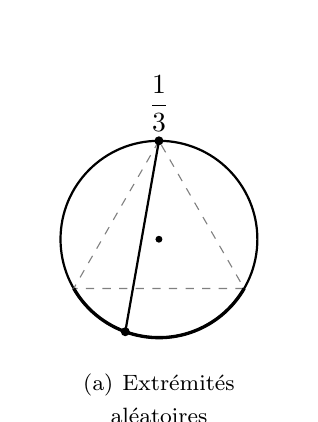
\begin{tikzpicture}[scale=1.25,>=stealth]
    \draw[thick] (0,0) circle (1);
    % inscribed equilateral triangle
    \draw[gray,dashed] (90:1) -- (210:1) -- (330:1) -- cycle;
    % favourable arc
    \draw[very thick] (210:1) arc (210:330:1);
    % the random chord
    \draw[thick] (90:1) -- (250:1);
    \fill (90:1) circle (1.3pt);
    \fill (250:1) circle (1.3pt);
    \fill (0,0) circle (1.0pt);
    \node at (0,1.38) {$\dfrac{1}{3}$};
    \node[text width=3.1cm,align=center] at (0,-1.62)
      {\footnotesize (a) Extrémités aléatoires};
  \end{tikzpicture}
  \hfill
  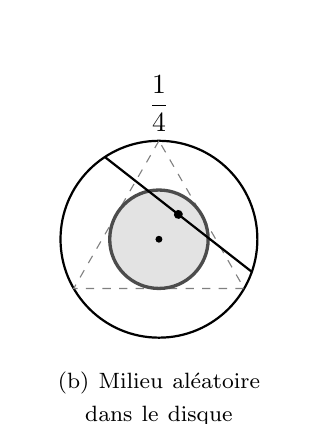
\begin{tikzpicture}[scale=1.25,>=stealth]
    \fill[gray!22] (0,0) circle (0.5);
    \draw[thick] (0,0) circle (1);
    \draw[gray,dashed] (90:1) -- (210:1) -- (330:1) -- cycle;
    \draw[very thick,gray!60!black] (0,0) circle (0.5);
    \begin{scope}[rotate=52]
      \draw[thick] (0.32,-0.947) -- (0.32,0.947);
      \fill (0.32,0) circle (1.3pt);
    \end{scope}
    \fill (0,0) circle (1.0pt);
    \node at (0,1.38) {$\dfrac{1}{4}$};
    \node[text width=3.1cm,align=center] at (0,-1.62)
      {\footnotesize (b) Milieu aléatoire dans le disque};
  \end{tikzpicture}
  \hfill
  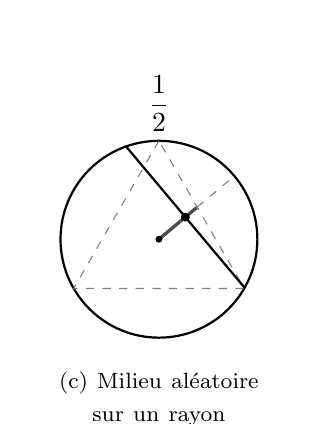
\begin{tikzpicture}[scale=1.25,>=stealth]
    \draw[thick] (0,0) circle (1);
    \draw[gray,dashed] (90:1) -- (210:1) -- (330:1) -- cycle;
    \begin{scope}[rotate=40]
      \draw[gray,dashed] (0,0) -- (1,0);
      \draw[very thick,gray!60!black] (0,0) -- (0.5,0);
      \draw[thick] (0.35,-0.937) -- (0.35,0.937);
      \fill (0.35,0) circle (1.3pt);
    \end{scope}
    \fill (0,0) circle (1.0pt);
    \node at (0,1.38) {$\dfrac{1}{2}$};
    \node[text width=3.1cm,align=center] at (0,-1.62)
      {\footnotesize (c) Milieu aléatoire sur un rayon};
  \end{tikzpicture}
\end{figure}

\medskip
Three constructions, three answers. Fix one endpoint of the chord at a vertex of
the inscribed triangle and draw the other endpoint uniformly on the circle: the
chord beats $\sqrt{3}$ exactly when the second endpoint falls on the opposite arc,
one third of the circle, so the answer is $1/3$. Draw instead the \emph{midpoint}
of the chord uniformly in the disc: the chord beats $\sqrt{3}$ exactly when its
midpoint lies within $1/2$ of the centre, an area ratio of $(1/2)^{2} = 1/4$. Draw
a radius, then the midpoint uniformly \emph{on that radius}: the condition is that
the midpoint falls in the inner half, so the answer is $1/2$.\\

None of the three is wrong. Le problème est en réalité mal posé car il faut
définir précisément la manière de tirer cette corde aléatoire: the three
constructions are three different questions wearing the same words. Ainsi la
définition précise de l'expérience aléatoire considérée est cruciale: the paradox
shows that \emph{at random} names nothing until it has been specified --- which
outcomes are possible, which collections of outcomes count as événements, and what
number each of those collections is assigned.
Those three things are the univers, the \textbf{tribu} (\textit{$\sigma$-algebra})
and the mesure, and building them is what this chapter does. Le calcul des
probabilités était un problème considéré si important et si difficile à l'époque
que David Hilbert y consacra un problème (le sixième) parmi sa liste de 23 problèmes
présentés en 1900. Une réponse à ce problème fut donnée dans les années 1930 par
Andreï Kolmogorov, avec une axiomatisation des probabilités reposant sur la théorie
de la mesure et de l'intégration, développée entre-temps par Émile Borel et Henri
Lebesgue, notamment.\\

Le terme de \textbf{mesure} (\textit{measure}) doit être compris comme une
formalisation des notions physiques de volume, d'aire ou de longueur : c'est une
application qui, à un ensemble, associe un nombre positif, éventuellement infini.
Si cet ensemble s'écrit comme une union de sous-ensembles disjoints, sa mesure doit
être égale à la somme des mesures de ces sous-ensembles. C'est la propriété de
$\sigma$-additivité, qui est au cœur de la notion de mesure. Une mesure classique
sur $\reals$ est la \textbf{mesure de Lebesgue} (\textit{Lebesgue measure}), notée
$\lambda$, qui satisfait $\lambda([a,b]) = b - a$.\\

Si une telle mesure semble très naturelle, sa construction est délicate, and the
delicacy cannot be waved away. \emph{Ainsi, en admettant l'axiome du choix, il
n'existe pas une telle mesure de ``longueur'' qui s'applique à tout sous-ensemble de
$\reals$.} Some subsets of the line cannot be assigned a length at all without
contradiction --- the Vitali set, built by choosing one representative from each
class of $[0,1]$ modulo $\mathbb{Q}$, is one. On doit restreindre le domaine de
définition de $\lambda$ à certains sous-ensembles, à savoir la tribu de Borel: a
family closed enough to be useful and small enough to be consistent. Everything
below that looks like bureaucracy --- why a tribu rather than all subsets, why a
mesure is defined on a tribu and not on $\mathcal{P}(\Omega)$ --- follows from that
one sentence.

\begin{notation}[Five deliberate collisions]
  The course's notation is used throughout these notes, collisions included. Five
  symbols carry more than one meaning, and each time the meaning is fixed by what
  sits in the parentheses:
  \begin{itemize}
    \item $\mathcal{P}$ is the \emph{ensemble des parties} $\mathcal{P}(\Omega)$ and
      the \emph{loi de Poisson} $\mathcal{P}(\lambda)$;
    \item $\mathcal{B}$ is the tribu de \emph{Borel} $\mathcal{B}(\reals)$, the loi
      de \emph{Bernoulli} $\mathcal{B}(p)$, the loi \emph{binomiale}
      $\mathcal{B}(n,p)$ and the loi \emph{Beta}
      $\mathcal{B}(a,b)$;
    \item $\lambda$ is the \emph{mesure de Lebesgue} and the parameter of the loi
      exponentielle and the loi de Poisson;
    \item $\Gamma$ is the \emph{loi Gamma} $\Gamma(a,\lambda)$ and the
      \emph{matrice de covariance} of a vecteur gaussien, $\mathcal{N}(\mu,\Gamma)$;
    \item $\mathcal{E}$ is a \emph{generic tribu}, as in $(E,\mathcal{E})$, and the
      \emph{loi exponentielle} $\mathcal{E}(\lambda)$.
  \end{itemize}
  An espace mesurable is written $(\Omega,\mathcal{F})$, an espace de probabilité
  $(\Omega,\mathcal{F},\prob)$, and generic espaces mesurables $(E,\mathcal{E})$ and
  $(F,\mathcal{F})$. The complement of $A$ is $A^{c}$.
\end{notation}

\begin{notation}[Set identities used without comment]
  Soit $A$, $B$, $C$ des ensembles :
  \begin{itemize}
    \item (commutativité) $A \union B = B \union A$,
      $A \intersect B = B \intersect A$ ;
    \item (associativité) $A \union (B \union C) = (A \union B) \union C$,
      $A \intersect (B \intersect C) = (A \intersect B) \intersect C$ ;
    \item (distributivité) $(A \union B) \intersect C = (A \intersect C) \union
      (B \intersect C)$, $(A \intersect B) \union C = (A \union C) \intersect
      (B \union C)$ ;
    \item (lois de Morgan) $(A \union B)^{c} = A^{c} \intersect B^{c}$,
      $(A \intersect B)^{c} = A^{c} \union B^{c}$.
  \end{itemize}
  Ces résultats s'étendent à des familles au plus dénombrables d'ensembles. De
  Morgan in its countable form is what makes ``stable under complement and
  countable union'' the same condition as ``stable under complement and countable
  intersection'', and it is used silently in almost every proof below.
\end{notation}

\subsection{Tribus}

Soit $\Omega$ un ensemble arbitraire.

\begin{definition}[Tribu]
  Une famille $\mathcal{F}$ de sous-ensembles de $\Omega$ est appelée une tribu sur
  $\Omega$ si elle vérifie les propriétés suivantes :
  \begin{itemize}
    \item $\Omega \in \mathcal{F}$ ;
    \item pour tout $A \in \mathcal{F}$, $A^{c} \in \mathcal{F}$ ;
    \item pour tous $A_{1}, A_{2}, \ldots \in \mathcal{F}$,
      $\bigcup_{i \geq 1} A_{i} \in \mathcal{F}$.
  \end{itemize}
\end{definition}

Autrement dit, une tribu contient $\Omega$, est stable par passage au
complémentaire et par union dénombrable. En passant au complémentaire, on obtient
qu'une tribu contient $\emptyset$ et est stable par intersection dénombrable.
Countable, not merely
finite, union is the essential clause: it is what puts the limit $\bigcup_{n} A_{n}$
of an increasing sequence inside $\mathcal{F}$, and every continuity and uniqueness
argument below passes through such a limit.

\begin{remark}[The two evident tribus]
  Every $\Omega$ carries two. The \textbf{tribu grossière} (\textit{coarse
  $\sigma$-algebra}) $\mathcal{F} = \{\emptyset, \Omega\}$ is the smallest, the
  \textbf{tribu des parties} (\textit{power-set $\sigma$-algebra}) $\mathcal{F} =
  \mathcal{P}(\Omega)$ is the largest, and every tribu on $\Omega$ sits between
  them. On a countable $\Omega$ one takes $\mathcal{P}(\Omega)$ and loses nothing;
  the difficulty is the uncountable case, where $\mathcal{P}(\reals)$ is too large
  to carry a length.
\end{remark}

\begin{definition}[Espace mesurable]
  Un espace $\Omega$ muni d'une tribu $\mathcal{F}$ s'appelle un
  \textbf{espace mesurable} (\textit{measurable space}), noté
  $(\Omega,\mathcal{F})$.
\end{definition}

\subsubsection{Trace}

Soit $(\Omega,\mathcal{F})$ un espace mesurable et $A \subr \Omega$. Nothing
requires $A$ itself to be in $\mathcal{F}$.

\begin{definition}[Trace]
  On appelle \textbf{trace} de $\mathcal{F}$ sur $A$ l'ensemble :
  \[
    \mathcal{F}_{A} = \{A \intersect B, \; B \in \mathcal{F}\}.
  \]
\end{definition}

\begin{prop}
  L'ensemble $\mathcal{F}_{A}$ est une tribu sur $A$.
\end{prop}

\begin{remark}
  Three checks, each one line. On vérifie que $A \in \mathcal{F}_{A}$ puisque $A =
  A \intersect \Omega$ avec $\Omega \in \mathcal{F}$. Le complémentaire de $A
  \intersect B$ \emph{dans $A$} est $A \intersect B^{c}$, qui appartient à
  $\mathcal{F}_{A}$ car $B^{c} \in \mathcal{F}$ --- the complement is taken in $A$,
  not in $\Omega$, which is why the trace is a tribu on $A$. And $\bigcup_{i \geq
  1}(A \intersect B_{i}) = A \intersect \bigcup_{i \geq 1} B_{i}$ by distributivity.
  On remarque que si $A \in \mathcal{F}$ alors $\mathcal{F}_{A} \subr \mathcal{F}$.
\end{remark}

\begin{example}[The trace of a three-point tribu]
  Soit $\Omega = \{1,2,3\}$ et $\mathcal{F} = \{\emptyset, \{1,2\}, \{3\},
  \{1,2,3\}\}$. Intersecting each of the four with $\{1,2\}$ gives $\emptyset$,
  $\{1,2\}$, $\emptyset$, $\{1,2\}$: la trace de $\mathcal{F}$ sur $\{1,2\}$ est la
  tribu grossière $\{\emptyset,\{1,2\}\}$ de $\{1,2\}$. A trace never distinguishes
  points that $\mathcal{F}$ did not distinguish.
\end{example}

\subsubsection{Tribu engendrée}

Nous allons définir la plus petite tribu contenant une collection d'ensembles.
Nous aurons besoin du résultat préliminaire suivant :

\begin{prop}
  Toute intersection de tribus sur $\Omega$ est une tribu sur $\Omega$.
\end{prop}

\begin{remark}
  Soit $(\mathcal{F}_{i})_{i \in I}$ une famille de tribus et $\mathcal{F}$ leur
  intersection. Each clause is inherited pointwise in $i$: $\Omega \in
  \mathcal{F}_{i}$ pour tout $i$ ; pour tout $A \in \mathcal{F}$, on a $A \in
  \mathcal{F}_{i}$ pour tout $i$, de sorte que $A^{c} \in \mathcal{F}_{i}$ pour tout
  $i$, soit $A^{c} \in \mathcal{F}$ ; same for countable unions. The index family
  $I$ may be uncountable --- no countability is used on it.
\end{remark}

\begin{definition}[Tribu engendrée]
  Soit $\mathcal{C} \subr \mathcal{P}(\Omega)$ une collection de sous-ensembles de
  $\Omega$. L'intersection de toutes les tribus contenant $\mathcal{C}$ est une
  tribu, appelée la \textbf{tribu engendrée} (\textit{generated $\sigma$-algebra})
  par $\mathcal{C}$. On la note $\sigma(\mathcal{C})$.
\end{definition}

The intersection is over a non-empty family, since $\mathcal{P}(\Omega)$ always
contains $\mathcal{C}$. By construction $\sigma(\mathcal{C})$ is the smallest tribu
containing $\mathcal{C}$: any tribu containing $\mathcal{C}$ contains
$\sigma(\mathcal{C})$. That is the only tool available for proving an inclusion
between tribus, and it is used in every proof of this chapter.

\begin{example}[The tribu generated by one set]
  Soit $\mathcal{C} = \{A\}$ avec $A \subr \Omega$. Alors $\sigma(\mathcal{C}) =
  \{\emptyset, \Omega, A, A^{c}\}$: those four are forced, and they already form a
  tribu.
\end{example}

\begin{example}[A tribu generated by two sets]
  Soit $\Omega = \{1,2,3,4\}$ et $\mathcal{C} = \{\{1\},\{2,3\}\}$. Complements give
  $\{2,3,4\}$ and $\{1,4\}$; unions give $\{1,2,3\}$ and, by complement, $\{4\}$.
  The list closes:
  \[
    \sigma(\mathcal{C}) = \bigl\{\emptyset, \{1\}, \{2,3\}, \{4\}, \{1,2,3\},
    \{1,4\}, \{2,3,4\}, \Omega\bigr\}.
  \]
  It has $2^{3} = 8$ elements, as expected: $\mathcal{C}$ splits $\Omega$ into the
  three atoms $\{1\}$, $\{2,3\}$, $\{4\}$, and a tribu generated by a finite
  partition is the set of unions of its atoms. The points $2$ and $3$ are never
  separated, so no tribu built from $\mathcal{C}$ can tell them apart.
\end{example}

\begin{example}[Tribu engendrée sur un intervalle]
  Soit $\Omega = [-1,1]$ et $\mathcal{C} = \{\{0\},[0,1]\}$. Par passage au
  complémentaire et union, on trouve
  \[
    \sigma(\mathcal{C}) = \bigl\{\emptyset, \{0\}, [0,1], \,]0,1], \,[-1,0],
    \,[-1,0[, \,[-1,0[ \,\union\, ]0,1], \,\Omega\bigr\},
  \]
  again eight sets, generated by the three atoms $[-1,0[$, $\{0\}$ and $]0,1]$.
\end{example}

\subsubsection{Tribu de Borel sur $\reals$}

\begin{definition}[Tribu de Borel]
  La \textbf{tribu de Borel} (\textit{Borel $\sigma$-algebra}) sur $\reals$, notée
  $\mathcal{B}(\reals)$, est la tribu sur $\reals$ engendrée par les intervalles
  $[a,b]$ avec $a < b$.
\end{definition}

Un élément de $\mathcal{B}(\reals)$ s'appelle un \textbf{borélien} (\textit{Borel
set}). En utilisant les propriétés d'une tribu (passage au complémentaire, union
et intersection dénombrables), on obtient que $\mathcal{B}(\reals)$ contient :
\begin{itemize}
  \item les intervalles $[a,b]$ pour tous $a < b$ ;
  \item les intervalles $[a,+\infty[$ et $]-\infty,b]$ ;
  \item les intervalles $]a,b]$, $[a,b[$ et $]a,b[$ ;
  \item les singletons $\{a\}$ ;
  \item les rationnels $\mathbb{Q}$ et les irrationnels $\reals \setminus \mathbb{Q}$.
\end{itemize}
La liste n'est pas exhaustive. En réalité, il est difficile d'exhiber un ensemble
qui ne soit pas un borélien --- in practice one never meets a subset of $\reals$
that fails to be one. Cela nécessite l'axiome du choix: the Vitali set of the
opening. That is the precise sense in which restricting to $\mathcal{B}(\reals)$
costs nothing in applications.

\begin{prop}[Génération par les demi-droites]
  La tribu de Borel $\mathcal{B}(\reals)$ est la tribu engendrée par les intervalles
  $]-\infty,b]$ pour tout $b \in \reals$.
\end{prop}

\begin{remark}
  Soit $\mathcal{C}$ cette collection. Each $]-\infty,b]$ is a borélien, de sorte
  que $\sigma(\mathcal{C}) \subr \mathcal{B}(\reals)$. Inversement,
  $\sigma(\mathcal{C})$ contient $]a,+\infty[$ par passage au complémentaire, et
  $[a,+\infty[ \; = \bigcap_{n \geq 1} \,]a - \tfrac{1}{n}, +\infty[$ par
  intersection dénombrable ; elle contient donc également $[a,b] = [a,+\infty[
  \,\intersect\, ]-\infty,b]$ par intersection, si bien que $\mathcal{B}(\reals)
  \subr \sigma(\mathcal{C})$. This is the generating family one actually uses: it is
  the reason the fonction de répartition determines a loi.
\end{remark}

\begin{prop}[Génération par les ouverts]
  La tribu de Borel $\mathcal{B}(\reals)$ est la tribu engendrée par les ouverts de
  $\reals$.
\end{prop}

\begin{proof}
  Soit $\mathcal{O}$ la collection des ouverts de $\reals$.\\

  \emph{First, $\sigma(\mathcal{O}) \subr \mathcal{B}(\reals)$.} Soit $U \in
  \mathcal{O}$. Pour tout $u \in U$, il existe des \emph{rationnels} $a_{u}, b_{u}$
  tels que $u \in [a_{u},b_{u}] \subr U$, because $U$ is open and $\mathbb{Q}$ is
  dense. En particulier,
  \[
    U = \bigcup_{u \in U} [a_{u},b_{u}].
  \]
  The union appears to be indexed by $U$, which is uncountable; but the intervals
  occurring in it have rational endpoints, and l'ensemble des intervalles à
  extrémités rationnelles est dénombrable. The union therefore has at most countably
  many distinct terms: c'est donc un borélien, comme union dénombrable de boréliens,
  and $U \in \mathcal{B}(\reals)$. Comme la tribu $\mathcal{B}(\reals)$ contient
  tous les ouverts, elle contient la tribu engendrée par les ouverts.\\

  \emph{Second, $\mathcal{B}(\reals) \subr \sigma(\mathcal{O})$.} Pour $a < b$,
  \[
    [a,b] = \bigcap_{n \geq 1} \;\Bigl]\,a - \frac{1}{n},\; b + \frac{1}{n}\,\Bigr[,
  \]
  a countable intersection of open sets. Donc $[a,b] \in \sigma(\mathcal{O})$.
  Comme la tribu $\sigma(\mathcal{O})$ contient tous les intervalles $[a,b]$, elle
  contient la tribu de Borel $\mathcal{B}(\reals)$.
\end{proof}

Two moves in that proof recur everywhere. Countability is smuggled in through
$\mathbb{Q}$: an uncountably indexed union collapses because only countably many
\emph{distinct} sets occur in it. And a closed set is reached from open sets by a
countable intersection.

\begin{remark}
  La caractérisation de la tribu de Borel comme la tribu engendrée par les ouverts
  permet d'étendre cette notion à des espaces de dimension infinie. It makes sense
  on any topological space, where ``interval'' has no meaning --- which is how one
  puts a tribu on a space of functions.
\end{remark}

\subsubsection{Tribu de Borel sur un intervalle, sur $\bar{\reals}$ et sur $\reals^{n}$}

\begin{definition}[Tribu de Borel sur un intervalle]
  La tribu de Borel sur un intervalle $[a,b]$, notée $\mathcal{B}([a,b])$, est la
  trace de $\mathcal{B}(\reals)$ sur $[a,b]$.
\end{definition}

Elle est constituée de l'ensemble des boréliens inclus dans $[a,b]$. La définition
s'étend à tout intervalle, ouvert ou fermé à droite ou à gauche, infini à droite ou
à gauche.

\begin{definition}[Tribu de Borel sur $\bar{\reals}$]
  Soit $\bar{\reals} = \reals \union \{-\infty,+\infty\}$. La tribu de Borel sur
  $\bar{\reals}$, notée $\mathcal{B}(\bar{\reals})$, est la tribu engendrée par les
  intervalles $[-\infty,b]$ pour tout $b \in \bar{\reals}$.
\end{definition}

Par rapport à $\mathcal{B}(\reals)$, cette tribu contient notamment les intervalles
$[-\infty,b]$ et $[a,+\infty]$ ainsi que les singletons $\{-\infty\}$ et
$\{+\infty\}$.

\begin{remark}[Why $\bar{\reals}$ is not a technicality]
  The two infinite points are admitted as genuine elements of the space, not as
  limits. That is what makes it legal to speak of a mesurable function taking the
  value $+\infty$ on a set of positive mesure. Two things later depend on it. The
  suprema, infima and upper and lower limits of a sequence of mesurable functions
  are mesurables \emph{as maps into $\bar{\reals}$}, and they generally have to be:
  $\sup_{n} f_{n}$ need not be finite anywhere. And the intégrale de Lebesgue of a
  positive mesurable function is defined with values in $[0,+\infty]$, so the
  théorème de convergence monotone can be stated without an integrability
  hypothesis. Dropping $\mathcal{B}(\bar{\reals})$ as a nicety costs both.
\end{remark}

\begin{definition}[Tribu de Borel sur $\reals^{n}$]
  Pour $n \geq 1$, la tribu de Borel sur $\reals^{n}$, notée
  $\mathcal{B}(\reals^{n})$, est la tribu sur $\reals^{n}$ engendrée par les
  \textbf{pavés} (\textit{boxes}) $[a_{1},b_{1}] \times \cdots \times [a_{n},b_{n}]$
  avec $a_{1} < b_{1}, \ldots, a_{n} < b_{n}$.
\end{definition}

Les deux propositions précédentes s'étendent à ce cas : $\mathcal{B}(\reals^{n})$
is equally generated by the sets $]-\infty,b_{1}] \times \cdots \times
\,]-\infty,b_{n}]$, and equally by the open sets of $\reals^{n}$.

\subsubsection{Tribu produit}

On se donne deux espaces mesurables $(E,\mathcal{E})$ et $(F,\mathcal{F})$ et on
cherche à construire une tribu sur l'espace produit $E \times F$. The obvious
candidate fails.

\begin{example}[The product of two tribus is not a tribu]
  Soit $\Omega = \{0,1\}$ et $\mathcal{F} = \mathcal{P}(\Omega)$. Alors $\mathcal{F}
  \times \mathcal{F}$, the family of rectangles $A \times B$, n'est pas une tribu de
  $\Omega \times \Omega$. En effet, le singleton $\{(0,0)\}$ is the rectangle $\{0\}
  \times \{0\}$ and so belongs to it, mais pas son complémentaire
  $\{(0,1),(1,0),(1,1)\}$, which is not a rectangle.
\end{example}

The rectangles must therefore be completed: il faut générer tous les autres
ensembles permettant de constituer une tribu, par passage au complémentaire et union
dénombrable --- which is to say, one generates.

\begin{definition}[Tribu produit]
  La \textbf{tribu produit} (\textit{product $\sigma$-algebra}), notée $\mathcal{E}
  \otimes \mathcal{F}$, est la tribu engendrée par $\mathcal{E} \times \mathcal{F}$.
\end{definition}

\begin{theorem}[La tribu de Borel de $\reals^{n}$ est la tribu produit]
  \[
    \mathcal{B}(\reals^{n}) = \mathcal{B}(\reals) \otimes \cdots \otimes
    \mathcal{B}(\reals) \qquad (n \text{ factors}).
  \]
\end{theorem}

\begin{proofsketch}
  On considère le cas $n = 2$. Le cas général se montre par récurrence. The
  inclusion $\mathcal{B}(\reals^{2}) \subr \mathcal{B}(\reals) \otimes
  \mathcal{B}(\reals)$ is immediate, since the right-hand side contains the pavés.
  The other inclusion is proved by a bootstrap that is worth recognising, because the
  same device reappears in the théorème d'unicité and in Fubini. On considère pour
  tout intervalle $A \subr \reals$ l'ensemble
  \[
    \mathcal{F} = \{B \in \mathcal{B}(\reals) : A \times B \in
    \mathcal{B}(\reals^{2})\}.
  \]
  On vérifie que $\mathcal{F}$ est une tribu --- $A \times B^{c} = (A \times \reals)
  \setminus (A \times B)$ and $A \times \bigcup_{i} B_{i} = \bigcup_{i} (A \times
  B_{i})$ --- and it contains the intervals, so it is all of $\mathcal{B}(\reals)$.
  Now fix a borélien $B$ and run the argument again on $\mathcal{G} = \{A \in
  \mathcal{B}(\reals) : A \times B \in \mathcal{B}(\reals^{2})\}$, which by the first
  step contains the intervals and is a tribu, hence is $\mathcal{B}(\reals)$.
  Finalement, $A \times B \in \mathcal{B}(\reals^{2})$ pour tous boréliens $A$, $B$,
  and the tribu produit they generate is contained in $\mathcal{B}(\reals^{2})$.
\end{proofsketch}

The device: to prove a property for all pairs of boréliens, freeze one argument,
show that the good values of the other form a tribu containing a generating family,
then unfreeze. One variable at a time, never both at once.

\subsection{Mesures}

Soit $(\Omega,\mathcal{F})$ un espace mesurable.

\begin{definition}[Mesure]
  Une \textbf{mesure} sur $(\Omega,\mathcal{F})$ est une fonction $\mu :
  \mathcal{F} \to [0,+\infty]$ telle que
  \begin{itemize}
    \item $\mu(\emptyset) = 0$ ;
    \item pour toute famille au plus dénombrable $(A_{i})_{i \in I}$ d'éléments de
      $\mathcal{F}$ deux-à-deux disjoints,
      \[
        \mu\Bigl(\bigcup_{i \in I} A_{i}\Bigr) = \sum_{i \in I} \mu(A_{i}).
      \]
  \end{itemize}
\end{definition}

\begin{figure}[h!]
  \centering
  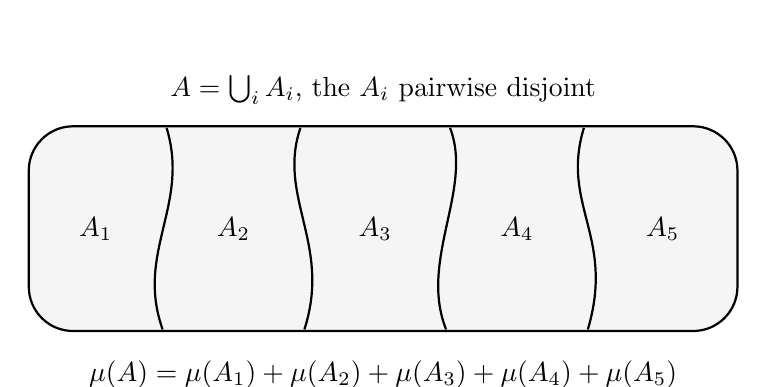
\begin{tikzpicture}[scale=1.0,>=stealth]
    \draw[thick,rounded corners=16pt,fill=gray!8] (0,0) rectangle (9,2.6);
    \draw[thick] (1.7,0.02) .. controls (1.35,1.0) and (2.05,1.6) .. (1.75,2.58);
    \draw[thick] (3.5,0.02) .. controls (3.85,1.1) and (3.15,1.7) .. (3.45,2.58);
    \draw[thick] (5.3,0.02) .. controls (4.95,0.9) and (5.65,1.8) .. (5.35,2.58);
    \draw[thick] (7.1,0.02) .. controls (7.45,1.2) and (6.75,1.6) .. (7.05,2.58);
    \node at (0.85,1.3) {$A_{1}$};
    \node at (2.6,1.3) {$A_{2}$};
    \node at (4.4,1.3) {$A_{3}$};
    \node at (6.2,1.3) {$A_{4}$};
    \node at (8.05,1.3) {$A_{5}$};
    \node[above] at (4.5,2.75) {$A = \bigcup_{i} A_{i}$, the $A_{i}$ pairwise disjoint};
    \node[below] at (4.5,-0.25)
      {$\mu(A) = \mu(A_{1}) + \mu(A_{2}) + \mu(A_{3}) + \mu(A_{4}) + \mu(A_{5})$};
  \end{tikzpicture}
\end{figure}

\medskip
On notera que la mesure d'un ensemble est une quantité positive, éventuellement
infinie; $[0,+\infty]$, not $[0,+\infty[$, is the target on purpose. Une mesure
$\mu$ est dite \emph{finie} si $\mu(\Omega) < \infty$. Additivity is required for
countable families and not merely finite ones, and only for \emph{pairwise disjoint}
sets --- weakening either restriction breaks the theory.

\begin{example}[Mesure de comptage]
  Soit $\Omega$ un ensemble. La fonction $\mu(A) = \operatorname{card}(A)$ est une
  mesure sur $(\Omega,\mathcal{P}(\Omega))$, appelée la \textbf{mesure de comptage}
  (\textit{counting measure}). It is finite exactly when $\Omega$ is finite.
\end{example}

\begin{example}[Mesure de Dirac]
  Soit $(\Omega,\mathcal{F})$ un espace mesurable et $a \in \Omega$. La fonction
  \[
    \delta_{a}(A) =
    \begin{cases}
      1 & \text{if } a \in A,\\
      0 & \text{otherwise,}
    \end{cases}
    \qquad A \in \mathcal{F},
  \]
  est une mesure, appelée la \textbf{mesure de Dirac} (\textit{Dirac measure}) en
  $a$. It is a mesure de probabilité: $\delta_{a}(\Omega) = 1$.
\end{example}

On vérifie facilement que toute somme au plus dénombrable de mesures est une
mesure: the check swaps two positive sums.

\begin{example}[Mesure de comptage de $\mathbb{N}$]
  La fonction $\mu = \sum_{n \in \mathbb{N}} \delta_{n}$ est une mesure sur
  $(\reals,\mathcal{B}(\reals))$: $\mu(A)$ counts the integers lying in $A$. Elle est
  appelée la mesure de comptage de $\mathbb{N}$, and it is the mesure with respect
  to which a sum over $\mathbb{N}$ will later be read as an integral.
\end{example}

\begin{definition}[Mesure $\sigma$-finie]
  Une mesure $\mu$ sur $(\Omega,\mathcal{F})$ est dite \textbf{$\sigma$-finie}
  (\textit{$\sigma$-finite}) si $\Omega$ peut être couvert par une réunion
  dénombrable d'ensembles de mesures finies.
\end{definition}

\begin{example}[$\sigma$-finite but not finite]
  La mesure de comptage de $\mathbb{N}$ sur $(\reals,\mathcal{B}(\reals))$ est
  $\sigma$-finie, en remarquant que $\reals = \bigcup_{n \geq 1} [-n,n]$ --- each
  $[-n,n]$ carries finitely many integers. Par contre, cette mesure n'est pas finie :
  $\mu(\reals) = +\infty$. The mesure de Lebesgue is $\sigma$-finie for the same
  covering, and also not finite.
\end{example}

$\sigma$-finiteness is the hypothesis that lets a statement about finite mesures be
transported to an infinite one by exhausting $\Omega$ along an increasing sequence.
It is close to, but weaker than, the covering hypothesis of the théorème d'unicité
below --- there the covering sets are required to lie in $\mathcal{C}$ itself --- and
it is a hypothesis of Fubini; when a result about mesures fails, the failure is
usually here.

\begin{prop}[Inclusion-exclusion et monotonie]
  Soit $\mu$ une mesure sur $(\Omega,\mathcal{F})$. Pour tous $A, B \in \mathcal{F}$,
  \begin{enumerate}
    \item $\mu(A \union B) + \mu(A \intersect B) = \mu(A) + \mu(B)$ ;
    \item si $A \subr B$, alors $\mu(A) \leq \mu(B)$.
  \end{enumerate}
\end{prop}

\begin{remark}
  Both come from $\sigma$-additivité applied to a decomposition into disjoint
  pieces. For the first, $A \union B = A \,\dunion\, (B \setminus A)$ gives
  $\mu(A \union B) + \mu(A \intersect B) = \mu(A) + \mu(B \setminus A) + \mu(A
  \intersect B) = \mu(A) + \mu(B)$, the last step because $B = (B \setminus A)
  \,\dunion\, (A \intersect B)$. For the second, $B = A \,\dunion\, (B
  \setminus A)$ and $\mu(B \setminus A) \geq 0$. Notice that the first identity is
  stated as a sum, not as $\mu(A \union B) = \mu(A) + \mu(B) - \mu(A \intersect B)$:
  the subtracted form is meaningless when $\mu(A \intersect B) = +\infty$. The
  additive form holds always.
\end{remark}

\subsubsection{Convergence monotone}

Une suite $(A_{n})_{n \geq 1}$ d'éléments de $\mathcal{F}$ est dite
\emph{croissante} si $A_{n} \subr A_{n+1}$ pour tout $n$ ; sa limite est alors $A =
\bigcup_{n} A_{n}$, ce que l'on notera $A_{n} \uparrow A$. De même, elle est dite
\emph{décroissante} si $A_{n+1} \subr A_{n}$ pour tout $n$ ; sa limite est $A =
\bigcap_{n} A_{n}$, ce que l'on notera $A_{n} \downarrow A$.

\begin{prop}[Continuité monotone, borne de l'union]
  Soit $\mu$ une mesure sur $(\Omega,\mathcal{F})$ et $(A_{n})_{n \geq 1}$ une suite
  d'éléments de $\mathcal{F}$.
  \begin{enumerate}
    \item Si $A_{n} \uparrow A$, alors $\mu(A) = \lim_{n} \uparrow \mu(A_{n})$.
    \item Si $A_{n} \downarrow A$ \textbf{et $\mu(A_{1}) < \infty$}, alors $\mu(A) =
      \lim_{n} \downarrow \mu(A_{n})$.
    \item On a la borne de l'union :
      $\displaystyle \mu\Bigl(\bigcup_{n \geq 1} A_{n}\Bigr) \leq \sum_{n \geq 1}
      \mu(A_{n})$, for any sequence, disjoint or not.
  \end{enumerate}
\end{prop}

\begin{remark}
  Continuity from below is $\sigma$-additivité in disguise: write $A = A_{1}
  \,\dunion\, (A_{2} \setminus A_{1}) \,\dunion\, \cdots$ and read the
  telescoping series as the limit of its partial sums. Continuity from above follows
  by passing to complements inside $A_{1}$, which is where the finiteness enters ---
  the step subtracts $\mu(A_{n})$ from $\mu(A_{1})$, and subtraction is not defined
  when both are $+\infty$. The borne de l'union follows from the disjointification
  $\bigcup_{n} A_{n} = \bigcup_{n} \bigl(A_{n} \setminus \bigcup_{k<n} A_{k}\bigr)$
  together with monotonicity.
\end{remark}

\begin{example}[Continuity from above fails without the finiteness hypothesis]
  Soit $\lambda$ la mesure de Lebesgue sur $\reals$ et $A_{n} = [n,+\infty[$ pour
  $n \geq 1$. The sequence is decreasing, and $\bigcap_{n \geq 1} A_{n} = \emptyset$,
  so $A_{n} \downarrow \emptyset$. Then
  \[
    \lambda\bigl(\lim_{n} \downarrow A_{n}\bigr) = \lambda(\emptyset) = 0,
    \qquad\text{whereas}\qquad
    \lim_{n} \downarrow \lambda(A_{n}) = +\infty,
  \]
  since $\lambda(A_{n}) = +\infty$ for every $n$. The two are not equal. The
  hypothesis $\mu(A_{1}) < \infty$ is violated --- $\lambda(A_{1}) = +\infty$ --- and
  the conclusion is false; the mass escapes to infinity rather than being destroyed.
  Dropping that one-line hypothesis is the classic error of the chapter, and this is
  the counter-example that catches it. Note that it is $\mu(A_{1})$, not $\mu(A)$,
  that must be finite: here $\mu(A) = 0$ and the conclusion still fails.
\end{example}

\subsubsection{Unicité}

Lorsque la tribu est engendrée par une collection d'ensembles (comme la tribu de
Borel, by the intervals), il est naturel de définir la mesure uniquement sur cette
collection d'ensembles, la mesure des autres ensembles s'en déduisant par
$\sigma$-additivité. Le \textbf{théorème d'unicité} (\textit{uniqueness theorem})
permet de formaliser cette idée.

\begin{theorem}[Unicité]
  Soit $\mu$ une mesure sur l'espace mesurable $(\Omega,\mathcal{F})$, avec
  $\mathcal{F} = \sigma(\mathcal{C})$ pour une certaine collection $\mathcal{C} \subr
  \mathcal{P}(\Omega)$. On suppose que :
  \begin{itemize}
    \item $\mathcal{C}$ est \textbf{stable par intersection finie}
      (\textit{stable under finite intersection}) --- a \emph{$\pi$-system} ---,
    \item $\Omega$ peut être couvert par une union dénombrable d'éléments de
      $\mathcal{C}$ de mesures finies.
  \end{itemize}
  S'il existe une mesure $\nu$ qui coïncide avec $\mu$ sur $\mathcal{C}$ alors $\nu
  = \mu$.
\end{theorem}

\begin{proof}
  Soit $B_{n} \uparrow \Omega$ une suite d'éléments de $\mathcal{C}$ telle que
  $\mu(B_{n}) < \infty$ pour tout $n \geq 1$ --- an increasing sequence, which is how
  the covering hypothesis is used: $\mathcal{C}$ is assumed stable par intersection
  finie only, so the finite unions of a bare cover need not lie in $\mathcal{C}$ and
  the cover is taken increasing from the start --- as it already is in every
  application below, $\reals = \bigcup_{n \geq 1} [-n,n]$ being the model. Pour tout
  $n$ fixé, soit
  \[
    \mathcal{M} = \{A \in \mathcal{F} : \mu(A \intersect B_{n}) = \nu(A \intersect
    B_{n})\}.
  \]
  On vérifie que $\mathcal{M}$ est une \textbf{classe monotone} (\textit{monotone
  class}) --- it contains $\Omega$, it is stable under proper difference, and it
  is stable under increasing limits. The lemme de classe monotone and the notion
  itself are carried in the reference chapter.
  \begin{itemize}
    \item $\Omega \in \mathcal{M}$: indeed $\Omega \intersect B_{n} = B_{n} \in
      \mathcal{C}$, where $\mu$ and $\nu$ agree by hypothesis.
    \item Si $A, B \in \mathcal{M}$ tels que $A \subr B$, alors
      \[
        \mu\bigl((B \setminus A) \intersect B_{n}\bigr)
        = \mu(B \intersect B_{n}) - \mu(A \intersect B_{n})
        = \nu(B \intersect B_{n}) - \nu(A \intersect B_{n})
        = \nu\bigl((B \setminus A) \intersect B_{n}\bigr),
      \]
      si bien que $B \setminus A \in \mathcal{M}$. \emph{The two subtractions are
      legal only because $\mu(A \intersect B_{n}) \leq \mu(B_{n}) < \infty$}, and the
      same for $\nu$; this is the single place where the finite-mesure half of the
      covering hypothesis is used, and without it the step is $\infty - \infty$.
    \item If $A_{1}, A_{2}, \ldots \in \mathcal{M}$ with $A_{k} \uparrow A$, then
      $A_{k} \intersect B_{n} \uparrow A \intersect B_{n}$ and continuity from below
      gives
      \[
        \mu(A \intersect B_{n}) = \lim_{k \to +\infty} \mu(A_{k} \intersect B_{n})
        = \lim_{k \to +\infty} \nu(A_{k} \intersect B_{n})
        = \nu(A \intersect B_{n}),
      \]
      si bien que $A \in \mathcal{M}$.
  \end{itemize}
  Next, $\mathcal{C} \subr \mathcal{M}$: for $A \in \mathcal{C}$ the set $A
  \intersect B_{n}$ again belongs to $\mathcal{C}$, \emph{because $\mathcal{C}$ is
  stable par intersection finie}, and $\mu$ and $\nu$ agree on $\mathcal{C}$.
  Hence the classe monotone generated by $\mathcal{C}$ satisfies $\mathcal{M}(
  \mathcal{C}) \subr \mathcal{M}$. Mais par le lemme de classe monotone --- whose own
  hypothesis is, once more, that $\mathcal{C}$ is stable par intersection finie
  ---, $\mathcal{M}(\mathcal{C}) = \sigma(\mathcal{C}) = \mathcal{F}$. On en déduit
  que $\mathcal{M} = \mathcal{F}$, de sorte que
  \[
    \forall A \in \mathcal{F}, \qquad \mu(A \intersect B_{n}) = \nu(A \intersect
    B_{n}).
  \]
  Finally let $n \to +\infty$. Since $A \intersect B_{n} \uparrow A$, continuity from
  below gives $\mu(A) = \nu(A)$ pour tout $A \in \mathcal{F}$, ce qui signifie que
  $\mu = \nu$.
\end{proof}

\begin{remark}[Where each hypothesis is spent]
  Stability of $\mathcal{C}$ under finite intersection is used twice, and both uses
  are essential: once to know that $A \intersect B_{n}$ is still a set on which $\mu$
  and $\nu$ are known to agree, and once inside the lemme de classe monotone, which
  is false without it. The finite-mesure covering is used twice as well: to make the
  difference step a legal subtraction, and to exhaust $\Omega$ at the end. Two
  mesures agreeing on a generating family that is \emph{not} a $\pi$-system may
  differ --- the theorem is not a formality, and on an exam the first thing to check
  is that the collection offered is closed under intersection.
\end{remark}

\subsubsection{Mesure de Lebesgue}

\begin{definition}[Mesure de Lebesgue sur $\reals$]
  La mesure de Lebesgue sur $(\reals,\mathcal{B}(\reals))$ est l'unique mesure,
  notée $\lambda$, telle que pour tous réels $a < b$,
  \[
    \lambda([a,b]) = b - a.
  \]
\end{definition}

La preuve de l'existence d'une telle mesure est difficile: it is obtained by
building an outer mesure from countable coverings by intervals, showing that the
sets splitting every test set additively form a tribu containing the boréliens, and
restricting. L'unicité est une conséquence directe du théorème d'unicité. Il suffit
en effet de considérer la collection $\mathcal{C}$ des intervalles $[a,b]$ avec $a
\leq b$, complétée de $\emptyset$. Cette collection est stable par intersection
finie, since the intersection of two such intervals is again one or is empty, and
$\reals = \bigcup_{n \geq 1} [-n,n]$ is a countable cover by elements of finite
mesure. Toute autre mesure $\nu$ qui donne la mesure $b - a$ à l'intervalle $[a,b]$
est nécessairement égale à $\lambda$.

\begin{remark}[Three consequences, each a one-line computation]
  Pour tout $a \in \reals$, $\lambda(\{a\}) = 0$, en utilisant le fait que $\{a\} =
  \bigcap_{n \geq 1} [a - \tfrac{1}{n}, a + \tfrac{1}{n}]$ --- a decreasing limit
  with $\lambda([a-1,a+1]) = 2 < \infty$, so continuity from above applies and gives
  $\lim_{n} \tfrac{2}{n} = 0$. Then $\lambda(\mathbb{Q}) = 0$ par
  $\sigma$-additivité, $\mathbb{Q}$ being a countable union of singletons. And
  $\lambda(\reals \setminus \mathbb{Q}) = +\infty$, since
  $\lambda(\reals) = \lambda(\mathbb{Q}) + \lambda(\reals \setminus \mathbb{Q})$ and
  $\lambda(\reals) = +\infty$. A countable set is invisible to $\lambda$; an
  uncountable one need not be visible either, as the ensemble de Cantor shows below.
\end{remark}

\begin{prop}[Invariance par translation (\textit{translation invariance})]
  Pour tout borélien $A$ et tout $t \in \reals$, $\lambda(A + t) = \lambda(A)$.
\end{prop}

\begin{remark}
  First, $A + t$ is a borélien whenever $A$ is: $\{B - t : B \in
  \mathcal{B}(\reals)\}$ is a tribu containing the intervals, hence contains
  $\mathcal{B}(\reals)$. So $\lambda(A+t)$ is defined. Notons $\mu(A) =
  \lambda(A+t)$ pour $A \in \mathcal{B}(\reals)$. On vérifie que
  $\mu$ est une mesure --- translation preserves disjointness and countable unions
  --- and $\mu([a,b]) = \lambda([a+t,b+t]) = b-a$, so $\mu$ coïncide avec $\lambda$
  sur les intervalles. D'après le théorème d'unicité, $\mu = \lambda$. This is the
  standard use of the theorem: to identify two mesures, check them on a
  $\pi$-system and stop. Conversely, la mesure de Lebesgue est la \emph{seule}
  mesure $\sigma$-finie invariante par translation sur $(\reals,\mathcal{B}(\reals))$,
  à une constante multiplicative près; the constant is recovered as $\alpha =
  \mu([0,1[)$, which is finite precisely because $\mu$ is $\sigma$-finie, and one
  then propagates $\mu([0,x[) = \alpha x$ from $x \in \mathbb{N}$ to $x \in
  \mathbb{Q}_{+}$ and finally to $x \in \reals_{+}$ by monotone limits.
\end{remark}

\begin{definition}[Mesure de Lebesgue sur $\reals^{n}$]
  La mesure de Lebesgue sur $(\reals^{n},\mathcal{B}(\reals^{n}))$ est l'unique
  mesure, que l'on notera également $\lambda$, telle que pour tous réels $a_{1} <
  b_{1}, \ldots, a_{n} < b_{n}$,
  \[
    \lambda\bigl([a_{1},b_{1}] \times \cdots \times [a_{n},b_{n}]\bigr)
    = (b_{1}-a_{1}) \cdots (b_{n}-a_{n}).
  \]
\end{definition}

Cette mesure est également la seule mesure $\sigma$-finie invariante par translation
sur $\reals^{n}$, à une constante multiplicative près. The $\sigma$-finiteness is
not decoration: without it the characterisation is false, and it is what a
computation of the image of $\lambda$ under an invertible affine map has to check
first.

\begin{example}[A mesure that is neither Lebesgue nor atomic]
  On $(\reals,\mathcal{B}(\reals))$ put $\mu = \lambda + \delta_{0}$, a sum of two
  mesures and therefore a mesure. Then
  \[
    \mu(\{0\}) = 1, \quad \mu([0,1]) = 2, \quad \mu([-1,1]) = 3, \quad
    \mu([-1,0[) = 1, \quad \mu(\reals_{+}) = +\infty.
  \]
  Each is the Lebesgue length plus $1$ if $0$ is in the set. In $\reals^{2}$ with
  $\mu = \lambda + \delta_{(0,0)}$ the same reading gives $\mu(\{(0,0)\}) = 1$,
  $\mu([0,1]^{2}) = 2$, $\mu([-1,1]^{2}) = 5$, $\mu([-1,0[^{2}) = 1$ and
  $\mu(\reals_{+} \times \{0\}) = 1$, the last because that half-line has mesure de
  Lebesgue zero in the plane and contains the origin.
\end{example}

\subsection{Ensembles négligeables}

Soit $\mu$ une mesure sur $(\Omega,\mathcal{F})$.

\begin{definition}[Ensemble négligeable]
  Un ensemble $A \in \mathcal{F}$ est dit \textbf{négligeable} (\textit{negligible})
  si $\mu(A) = 0$.
\end{definition}

Une propriété est dite vraie \textbf{presque partout} (\textit{almost everywhere})
si sa négation correspond à un ensemble négligeable. The abbreviation p.p. is kept
in its French form, and it is the primary form in these notes; the mesure it refers
to is always named or clear from the context.

\begin{example}[Almost every real is irrational]
  Presque tout réel est irrationnel pour la mesure de Lebesgue: $\lambda(\mathbb{Q})
  = 0$, so the set of rationals is négligeable. There are as many rationals as
  integers and uncountably many reals, and $\lambda$ sees only the second fact.
\end{example}

\begin{remark}[Negligible with respect to which mesure?]
  Negligibility is a statement about a pair, a set \emph{and} a mesure: il faut
  veiller à bien spécifier la mesure considérée. Par exemple, il est faux de dire
  que presque tout réel est irrationnel pour la mesure $\mu = \lambda + \delta_{0}$:
  $\mu(\mathbb{Q}) \geq \mu(\{0\}) = 1 \neq 0$, so $\mathbb{Q}$ n'est pas
  négligeable pour $\mu$, even though it is for $\lambda$. Two mesures on the same
  tribu can disagree completely about which sets are négligeables.
\end{remark}

\begin{example}[An uncountable negligible set: the ensemble de Cantor]
  Let $C_{0} = [0,1[$, and let $C_{n+1}$ be obtained from $C_{n}$ by deleting the
  open middle third of each of its intervals, so that
  \[
    C_{1} = \Bigl[0,\tfrac{1}{3}\Bigr[ \,\union\, \Bigl[\tfrac{2}{3},1\Bigr[,
    \qquad
    C_{2} = \Bigl[0,\tfrac{1}{9}\Bigr[ \,\union\, \Bigl[\tfrac{2}{9},\tfrac{1}{3}
    \Bigr[ \,\union\, \Bigl[\tfrac{2}{3},\tfrac{7}{9}\Bigr[ \,\union\,
    \Bigl[\tfrac{8}{9},1\Bigr[,
  \]
  and set $C = \bigcap_{n \geq 0} C_{n}$, the \textbf{ensemble de Cantor}
  (\textit{Cantor set}). A real of $[0,1[$ lies in $C_{n}$ exactly when none of
  the first $n$ digits of its ternary expansion is $1$, so $C$ is the set of reals whose
  ternary expansion uses only the digits $0$ and $2$. Replacing every $2$ by a $1$
  maps $C$ bijectively onto the binary expansions, that is onto $[0,1[$: the
  ensemble de Cantor is uncountable. Yet $C_{n}$ is a union of $2^{n}$ intervals of
  length $3^{-n}$, so $\lambda(C_{n}) = (2/3)^{n}$, and $C_{n} \downarrow C$ with
  $\lambda(C_{0}) = 1 < \infty$, so continuity from above applies and
  \[
    \lambda(C) = \lim_{n} \left(\frac{2}{3}\right)^{n} = 0 .
  \]
  Being négligeable is therefore not a statement about cardinality. Note that the
  finiteness hypothesis was available here and had to be invoked.
\end{example}

\subsection{Fonctions mesurables}

Soit $(\Omega,\mathcal{F})$ et $(E,\mathcal{E})$ deux espaces mesurables.

\begin{definition}[Fonction mesurable]
  Une fonction $f : \Omega \to E$ est dite \textbf{mesurable} (\textit{measurable})
  si :
  \[
    \forall A \in \mathcal{E}, \qquad f^{-1}(A) \in \mathcal{F}.
  \]
\end{definition}

\begin{figure}[h!]
  \centering
  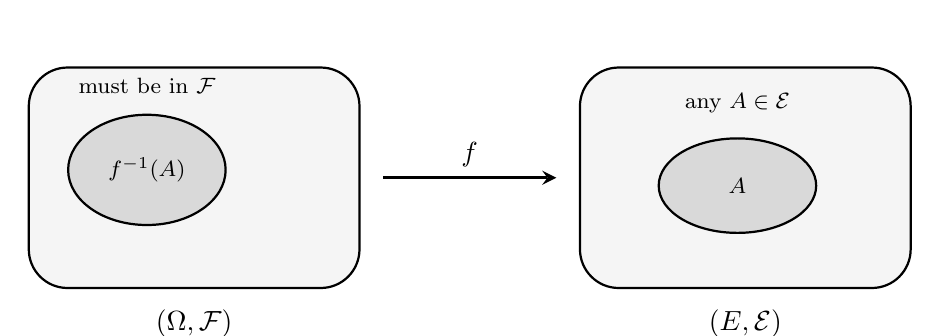
\begin{tikzpicture}[scale=1.0,>=stealth]
    \draw[thick,rounded corners=14pt,fill=gray!8] (0,0) rectangle (4.2,2.8);
    \draw[thick,rounded corners=14pt,fill=gray!8] (7.0,0) rectangle (11.2,2.8);
    \node[below] at (2.1,-0.15) {$(\Omega,\mathcal{F})$};
    \node[below] at (9.1,-0.15) {$(E,\mathcal{E})$};
    \draw[thick,fill=gray!30] (1.5,1.5) ellipse (1.0 and 0.7);
    \draw[thick,fill=gray!30] (9.0,1.3) ellipse (1.0 and 0.6);
    \node at (1.5,1.5) {\footnotesize $f^{-1}(A)$};
    \node at (9.0,1.3) {\footnotesize $A$};
    \draw[->,very thick] (4.5,1.4) -- (6.7,1.4) node[midway,above] {$f$};
    \node[above] at (1.5,2.35) {\footnotesize must be in $\mathcal{F}$};
    \node[above] at (9.0,2.1) {\footnotesize any $A \in \mathcal{E}$};
  \end{tikzpicture}
\end{figure}

\medskip
Measurability is a condition on \emph{preimages}, never on images, because $f^{-1}$
commutes with every set operation --- complement, arbitrary union, arbitrary
intersection --- while the direct image does not commute with complement. That one
algebraic fact makes the whole of this subsection work.

\begin{example}[The indicator function is measurable]
  Soit $A \in \mathcal{F}$. La fonction $f = \indic_{A}$ est mesurable de
  $(\Omega,\mathcal{F})$ vers $(\reals,\mathcal{B}(\reals))$. En effet, pour tout
  borélien $B$,
  \[
    f^{-1}(B) =
    \begin{cases}
      A & \text{if } 1 \in B, \; 0 \notin B,\\
      A^{c} & \text{if } 1 \notin B, \; 0 \in B,\\
      \Omega & \text{if } 0, 1 \in B,\\
      \emptyset & \text{if } 0, 1 \notin B,
    \end{cases}
  \]
  and all four are in $\mathcal{F}$. Only four preimages occur because $f$ takes only
  two values; measurability of $\indic_{A}$ is exactly the statement $A \in
  \mathcal{F}$.
\end{example}

\begin{remark}
  On remarque que si $\mathcal{F} = \mathcal{P}(\Omega)$ alors toute fonction sur
  $\Omega$ est mesurable, whatever the target. Measurability constrains only when the
  source tribu is genuinely smaller than the ensemble des parties: it measures how
  much information $\mathcal{F}$ carries about $f$.
\end{remark}

\begin{lemma}[La mesurabilité se vérifie sur une collection génératrice]
  Soit $\mathcal{C} \subr \mathcal{P}(E)$ une collection d'ensembles telle que
  $\mathcal{E} = \sigma(\mathcal{C})$. Une condition suffisante pour que $f : \Omega
  \to E$ soit mesurable est que :
  \[
    \forall A \in \mathcal{C}, \qquad f^{-1}(A) \in \mathcal{F}.
  \]
\end{lemma}

\begin{remark}
  Soit $\mathcal{G} = \{A \in \mathcal{E} : f^{-1}(A) \in \mathcal{F}\}$. It is a
  tribu, precisely because $f^{-1}$ commutes with complement and countable union:
  $f^{-1}(E) = \Omega$, $f^{-1}(A^{c}) = f^{-1}(A)^{c}$ and $f^{-1}(\bigcup_{i}
  A_{i}) = \bigcup_{i} f^{-1}(A_{i})$. Par hypothèse, $\mathcal{C} \subr
  \mathcal{G}$, donc $\mathcal{E} = \sigma(\mathcal{C}) \subr \mathcal{G}$, ce qui
  signifie que la fonction $f$ est mesurable. This lemma is the workhorse of the
  subsection: every measurability proof below applies it to a well-chosen generating
  family, and for a real-valued function that family is almost always the half-lines
  $]-\infty,b]$.
\end{remark}

\subsubsection{Mesure image}

Si $\mu$ est une mesure sur $(\Omega,\mathcal{F})$, toute fonction mesurable définit
une nouvelle mesure, transported to the target.

\begin{definition}[Mesure image]
  Soit $f : \Omega \to E$ une fonction mesurable. La mesure $\mu_{f}$ définie par :
  \[
    \forall A \in \mathcal{E}, \qquad \mu_{f}(A) = \mu\bigl(f^{-1}(A)\bigr)
  \]
  est appelée la \textbf{mesure image} (\textit{image measure}) de $\mu$ par $f$.
\end{definition}

That $\mu_{f}$ is a mesure is again the commutation of $f^{-1}$ with the set
operations: preimages of disjoint sets are disjoint, and a countable disjoint union
pulls back to one. This construction later carries the whole of probability --- the
loi of a variable aléatoire is the image of $\prob$ by that variable, and nothing
else.

\begin{example}[Mesure image sur un espace à deux points]
  Soit $\Omega = \{1,2,3\}$ et $\mu$ la mesure de comptage sur
  $(\Omega,\mathcal{P}(\Omega))$, and $f = \indic_{\{1,2\}}$ with values in $E =
  \{0,1\}$. Then $f^{-1}(\{0\}) = \{3\}$ and $f^{-1}(\{1\}) = \{1,2\}$, so
  \[
    \mu_{f}(\{0\}) = 1, \qquad \mu_{f}(\{1\}) = 2 .
  \]
  The total mass $3$ is preserved: a mesure image never creates or destroys mass,
  it only redistributes it.
\end{example}

\begin{example}[Mesure de Lebesgue et fonction affine]
  Soit $\phi : \reals \to \reals$ la fonction affine $\phi(x) = \alpha x + \beta$,
  avec \textbf{$\alpha \neq 0$}. Pour $a < b$,
  \[
    x \in \phi^{-1}([a,b])
    \iff a \leq \alpha x + \beta \leq b,
  \]
  on obtient l'intervalle $\bigl[\tfrac{a-\beta}{\alpha}, \tfrac{b-\beta}{\alpha}
  \bigr]$ si $\alpha > 0$ et l'intervalle $\bigl[\tfrac{b-\beta}{\alpha},
  \tfrac{a-\beta}{\alpha}\bigr]$ si $\alpha < 0$; in both cases its length is
  $(b-a)/|\alpha|$. On en déduit $\lambda_{\phi}([a,b]) = (b-a)/|\alpha|$, and the
  two mesures $\lambda_{\phi}$ and $\lambda/|\alpha|$ agree on the intervals, a
  $\pi$-system generating $\mathcal{B}(\reals)$ along a countable cover of finite
  mesure. By the théorème d'unicité,
  \[
    \lambda_{\phi} = \frac{\lambda}{|\alpha|} .
  \]
  The invertibility $\alpha \neq 0$ is essential: for $\alpha = 0$ the map is
  constant, the
  preimage of a set is $\emptyset$ or $\reals$, and the mesure image is not even
  $\sigma$-finie. In $\reals^{n}$ the same statement holds for $\phi(x) = Ax + b$
  with $A$ \textbf{invertible}, and reads $\lambda_{\phi} = \lambda/|\det A|$;
  the proof reduces the general case to the diagonal, orthogonal and symmetric ones
  through the polar decomposition $A = QS$, and the first step is precisely the
  check that $\lambda_{\phi}$ is $\sigma$-finie and translation-invariant.
\end{example}

\subsubsection{Stabilité de la mesurabilité}

\begin{prop}[Composition de fonctions]
  Soit $(G,\mathcal{G})$ un espace mesurable. Si les fonctions $f : \Omega \to E$ et
  $g : E \to G$ sont mesurables, la fonction $g \circ f : \Omega \to G$ est
  mesurable.
\end{prop}

\begin{remark}
  One line: pour tout ensemble $A \in \mathcal{G}$, on a $g^{-1}(A) \in \mathcal{E}$
  because $g$ is mesurable, donc $f^{-1}\bigl(g^{-1}(A)\bigr) \in \mathcal{F}$ because
  $f$ is; and $(g \circ f)^{-1}(A) = f^{-1}(g^{-1}(A))$.
\end{remark}

On s'intéresse maintenant aux fonctions réelles $f : \Omega \to \reals$ ou
vectorielles $f : \Omega \to \reals^{n}$, les ensembles $\reals$ et $\reals^{n}$
étant munis de leur tribu de Borel.

\begin{prop}[Continuité implique mesurabilité]
  Toute fonction continue $f : \Omega \to \reals^{n}$, avec $\Omega = \reals$ ou
  $\reals^{m}$ muni de sa tribu de Borel, est mesurable.
\end{prop}

\begin{remark}
  Under a continuous map, l'image réciproque d'un ouvert est un ouvert, hence a
  borélien; la tribu de Borel de $\reals^{n}$ étant engendrée par les ouverts,
  conclude by the generating lemma. This is the one place where the characterisation
  of $\mathcal{B}(\reals)$ by the open sets, rather than by the intervals, is what
  makes the argument work at all.
\end{remark}

\begin{remark}[The converse is false]
  Il existe des fonctions mesurables qui ne sont pas continues. Par exemple, la
  fonction $\indic_{\mathbb{Q}} : \reals \to \reals$ est mesurable puisque
  $\mathbb{Q}$ est un borélien, and is continuous at no point. Measurability is much
  weaker than continuity, and that weakness is the point: the class of mesurable
  functions is closed under operations --- limits above all --- under which the
  continuous functions are not.
\end{remark}

\begin{prop}[Mesurabilité coordonnée par coordonnée]
  Soit $f = (f_{1},\ldots,f_{n})$ une fonction de $\Omega$ vers $\reals^{n}$. La
  fonction $f$ est mesurable si et seulement si les fonctions $f_{1},\ldots,f_{n}$
  sont mesurables.
\end{prop}

\begin{remark}
  Forwards: $f_{1}^{-1}([a,b]) = f^{-1}([a,b] \times \reals \times \cdots \times
  \reals)$, a preimage of a borélien, so $f_{1}$ is mesurable by the generating
  lemma, and likewise for the other coordinates. Réciproquement, pour tout pavé,
  \[
    f^{-1}\bigl([a_{1},b_{1}] \times \cdots \times [a_{n},b_{n}]\bigr)
    = f_{1}^{-1}([a_{1},b_{1}]) \intersect \cdots \intersect
      f_{n}^{-1}([a_{n},b_{n}]),
  \]
  a finite intersection of elements of $\mathcal{F}$; the pavés generate
  $\mathcal{B}(\reals^{n})$, so the generating lemma applies again.
\end{remark}

\begin{prop}[Opérations algébriques]
  Si $f$ et $g$ sont des fonctions mesurables, alors les fonctions $f + g$, $fg$,
  $\max(f,g)$ et $\min(f,g)$ sont mesurables.
\end{prop}

\begin{remark}
  Each is a composition. La fonction addition $\reals^{2} \to \reals$, $(x,y) \mapsto
  x + y$, est continue donc mesurable; the pair $(f,g) : \Omega \to \reals^{2}$ is
  mesurable by coordinatewise measurability; so $f + g$ is mesurable as a
  composition of two mesurable maps. Multiplication, $\max$ and $\min$ are
  continuous in the same way: la preuve est identique pour les autres opérations.
  Note the order of the three propositions: composition, then coordinates, then
  operations --- each uses the one before.
\end{remark}

\begin{example}[Fonction mesurable sur $\reals$]
  La fonction $f(x) = x^{2} + \indic_{\reals_{+}}(x)$ est mesurable de
  $(\reals,\mathcal{B}(\reals))$ vers $(\reals,\mathcal{B}(\reals))$ : c'est la somme
  de deux fonctions mesurables, la fonction continue $x \mapsto x^{2}$, mesurable
  because continuous, et la fonction indicatrice du borélien $\reals_{+}$, mesurable
  because $\reals_{+}$ is a borélien. It is discontinuous at $0$, which costs nothing.
\end{example}

\begin{example}[Fonction mesurable sur $\reals^{2}$]
  Likewise, la fonction $f(x,y) = xy + \indic_{\{(0,0)\}}(x,y)$ est mesurable de
  $(\reals^{2},\mathcal{B}(\reals^{2}))$ vers $(\reals,\mathcal{B}(\reals))$ : c'est
  la somme de deux fonctions mesurables, la fonction continue $(x,y) \mapsto xy$ et
  la fonction indicatrice du singleton $\{(0,0)\}$, which is a borélien of
  $\reals^{2}$.
\end{example}

\subsubsection{Limites de fonctions mesurables}

Here the class of mesurable functions shows what it is for. Nous allons maintenant
considérer la limite d'une suite de fonctions mesurables, lorsqu'elle existe, et
montrer qu'on obtient une fonction mesurable. C'est une différence notable avec les
fonctions continues, la limite de fonctions continues n'étant pas continue en
général. Nous allons travailler sur l'ensemble $\bar{\reals}$, muni de sa tribu de
Borel $\mathcal{B}(\bar{\reals})$, since a supremum of real functions need not be
finite.

\begin{prop}[Supremum, infimum et limites]
  Soit $(f_{n})_{n \geq 1}$ une suite de fonctions mesurables de $\Omega$ vers
  $\bar{\reals}$. Alors les fonctions $\inf_{n} f_{n}$, $\sup_{n} f_{n}$,
  $\liminf_{n} f_{n}$, $\limsup_{n} f_{n}$ et $\lim_{n} f_{n}$ (lorsque celle-ci
  existe) sont des fonctions mesurables de $\Omega$ vers $\bar{\reals}$.
\end{prop}

\begin{remark}
  Soit $f = \sup_{n} f_{n}$. On a pour tout $b \in \bar{\reals}$ :
  \[
    f^{-1}\bigl([-\infty,b]\bigr) = \bigcap_{n \geq 1} f_{n}^{-1}
    \bigl([-\infty,b]\bigr) \in \mathcal{F},
  \]
  because $\sup_{n} f_{n}(\omega) \leq b$ if and only if $f_{n}(\omega) \leq b$ for
  every $n$. Comme $\mathcal{B}(\bar{\reals})$ est engendrée par les intervalles
  $[-\infty,b]$, la fonction $f$ est mesurable by the generating lemma. On montre de
  la même manière que l'infimum est mesurable, $\mathcal{B}(\bar{\reals})$ étant
  également engendrée par les intervalles $[a,+\infty]$. Then
  \[
    \liminf_{n} f_{n} = \sup_{n} \inf_{k \geq n} f_{k},
    \qquad
    \limsup_{n} f_{n} = \inf_{n} \sup_{k \geq n} f_{k},
  \]
  so both are mesurables by two applications of what precedes. Enfin, si la limite
  $\lim_{n} f_{n}$ est bien définie, elle vaut $\liminf_{n} f_{n}$, which settles it.
\end{remark}

\begin{remark}[Where $\bar{\reals}$ was needed]
  Nothing forces the sequence to be bounded, so $\sup_{n} f_{n}$ may legitimately be
  $+\infty$ on a set of positive mesure. Had the target been $\reals$, the
  proposition would have needed a boundedness hypothesis and would have been useless
  for the next chapter's théorème de convergence monotone and lemme de Fatou, both
  stated for positive mesurable functions with values in $[0,+\infty]$. This is why
  $\mathcal{B}(\bar{\reals})$ was defined at all.
\end{remark}

\begin{conclusion}
  The chapter fixes three objects and one theorem. The objects: a \emph{tribu}, which
  is the family of sets one is allowed to measure, generated in practice from a small
  collection --- intervals, half-lines, open sets, pavés --- rather than written out;
  a \emph{mesure}, a $\sigma$-additive map into $[0,+\infty]$, of which $\lambda$ and
  $\delta_{a}$ are the two models and all the rest are built from them; and a
  \emph{mesurable function}, defined by its preimages and therefore stable under
  composition, algebraic operations and, decisively, pointwise limits. The theorem is
  uniqueness: two mesures agreeing on a $\pi$-system that generates the tribu, with
  a countable cover of $\Omega$ by elements of that $\pi$-system of finite mesure,
  are equal --- which is what allows every later
  identification of a loi to stop after checking a generating family.\\

  Two hypotheses go missing under compression, and both were written out above:
  continuity from above needs $\mu(A_{1}) < \infty$, with $A_{n} = [n,+\infty[$ as
  the standing counter-example, and the théorème d'unicité needs $\mathcal{C}$ stable
  par intersection finie, used once to keep $A \intersect B_{n}$ inside
  $\mathcal{C}$ and once inside the lemme de classe monotone. The next chapter builds
  the integral on these objects, starting with positive mesurable functions valued in
  $[0,+\infty]$ --- the reason $\mathcal{B}(\bar{\reals})$ was defined here.
\end{conclusion}

\section{Intégrale de Lebesgue}

The previous chapter built three objects --- a tribu, a mesure, a mesurable
function --- and stopped just short of using them. This chapter uses them: nous
allons maintenant définir une intégrale par rapport à une mesure. C'est
l'\textbf{intégrale de Lebesgue} (\textit{Lebesgue integral}), beaucoup plus générale que l'intégrale de Riemann, in two
independent directions: elle permet d'intégrer beaucoup plus de fonctions, et par
rapport à n'importe quelle mesure, pas uniquement la mesure ``uniforme'' utilisée
habituellement, qui correspond à la mesure de Lebesgue.\\

The idea is a single change of axis. Riemann cuts the \emph{domain} into small
intervals and multiplies the width of each by a value of $f$ on it. Lebesgue cuts the
\emph{range} into small intervals and multiplies the length of each level band by the
mesure of the set of points where $f$ takes a value in that band. De manière
schématique, l'intégrale de Lebesgue est définie à partir d'une discrétisation selon
l'axe des ordonnées (les différentes valeurs prises par la fonction à intégrer)
plutôt que selon l'axe des abscisses (l'ensemble de définition de la fonction): that
is the whole of the construction; everything below is bookkeeping.

\begin{figure}[h!]
  \centering
  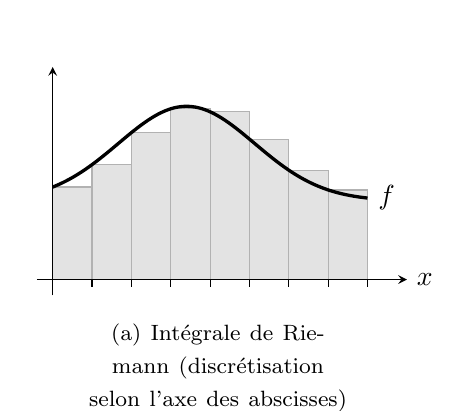
\begin{tikzpicture}[scale=1.0,>=stealth]
    % --- Riemann: vertical slabs ---
    \fill[gray!22] (0,0) rectangle (0.5,1.175);
    \fill[gray!22] (0.5,0) rectangle (1.0,1.459);
    \fill[gray!22] (1.0,0) rectangle (1.5,1.866);
    \fill[gray!22] (1.5,0) rectangle (2.0,2.168);
    \fill[gray!22] (2.0,0) rectangle (2.5,2.130);
    \fill[gray!22] (2.5,0) rectangle (3.0,1.783);
    \fill[gray!22] (3.0,0) rectangle (3.5,1.389);
    \fill[gray!22] (3.5,0) rectangle (4.0,1.138);
    \draw[gray!60] (0,0) rectangle (0.5,1.175);
    \draw[gray!60] (0.5,0) rectangle (1.0,1.459);
    \draw[gray!60] (1.0,0) rectangle (1.5,1.866);
    \draw[gray!60] (1.5,0) rectangle (2.0,2.168);
    \draw[gray!60] (2.0,0) rectangle (2.5,2.130);
    \draw[gray!60] (2.5,0) rectangle (3.0,1.783);
    \draw[gray!60] (3.0,0) rectangle (3.5,1.389);
    \draw[gray!60] (3.5,0) rectangle (4.0,1.138);
    \draw[->] (-0.2,0) -- (4.5,0) node[right] {$x$};
    \draw[->] (0,-0.2) -- (0,2.7);
    \draw[very thick,domain=0:4,samples=120,smooth]
      plot (\x,{1+1.2*exp(-(\x-1.7)*(\x-1.7)/1.5)}) node[right] {$f$};
    \foreach \t in {0,0.5,1.0,1.5,2.0,2.5,3.0,3.5,4.0}
      \draw (\t,0) -- (\t,-0.09);
    \node[text width=4.6cm,align=center] at (2.1,-1.12)
      {\footnotesize (a) Intégrale de Riemann (discrétisation selon l'axe des
       abscisses)};
  \end{tikzpicture}
  \hfill
  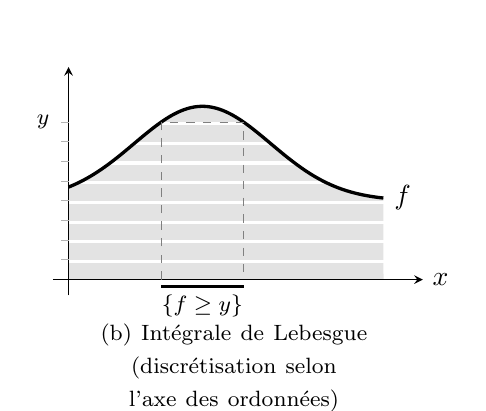
\begin{tikzpicture}[scale=1.0,>=stealth]
    % --- Lebesgue: horizontal bands ---
    \begin{scope}
      \clip (0,0) -- plot[domain=0:4,samples=120,smooth]
        (\x,{1+1.2*exp(-(\x-1.7)*(\x-1.7)/1.5)}) -- (4,0) -- cycle;
      \foreach \k in {0,1,2,3,4,5,6,7,8}
        \fill[gray!22] (0,{0.25*\k}) rectangle (4,{0.25*\k+0.21});
    \end{scope}
    \draw[->] (-0.2,0) -- (4.5,0) node[right] {$x$};
    \draw[->] (0,-0.2) -- (0,2.7);
    \draw[very thick,domain=0:4,samples=120,smooth]
      plot (\x,{1+1.2*exp(-(\x-1.7)*(\x-1.7)/1.5)}) node[right] {$f$};
    \foreach \k in {1,2,3,4,5,6,7,8}
      \draw[gray!60] (0,{0.25*\k}) -- (-0.09,{0.25*\k});
    % the level set of one band, read back on the x-axis
    \draw[very thick] (1.177,-0.09) -- (2.223,-0.09);
    \node at (1.70,-0.34) {\footnotesize $\{f \geq y\}$};
    \draw[gray,dashed] (1.177,0) -- (1.177,2.0) -- (2.223,2.0) -- (2.223,0);
    \node[left] at (-0.12,2.0) {\footnotesize $y$};
    \node[text width=4.6cm,align=center] at (2.1,-1.12)
      {\footnotesize (b) Intégrale de Lebesgue (discrétisation selon l'axe des
       ordonnées)};
  \end{tikzpicture}
  \vspace{0.5cm}
\end{figure}

\medskip
The price of the change is that the level set $\{f \geq y\}$ has to be mesurable for
its mesure to exist, which is why measurability was defined first. The reward is
that the class of integrable functions becomes stable under pointwise limits, and
that is what the three convergence theorems of this chapter say.

\subsection{Définition}

Soit $(\Omega,\mathcal{F})$ un espace mesurable.

\begin{definition}[Fonction étagée (\textit{simple function})]
  Une fonction $f$ mesurable de $(\Omega,\mathcal{F})$ vers
  $(\reals,\mathcal{B}(\reals))$ est dite \textbf{étagée} si elle prend un nombre
  fini de valeurs.
\end{definition}

Une telle fonction s'écrit :
\[
  f = \sum_{i=1}^{n} \alpha_{i} \indic_{A_{i}},
\]
où $\alpha_{1},\ldots,\alpha_{n}$ sont les valeurs distinctes et non-nulles prises
par $f$, et pour tout $i$, $A_{i} = f^{-1}(\{\alpha_{i}\})$. Notons que, la fonction
$f$ étant mesurable, each $A_{i}$ belongs to $\mathcal{F}$; this is the only place
measurability is used, and it is what makes the next definition legal. This
decomposition is called the canonical form, and it will be referred to below simply
as writing $f$ in the form above.

\begin{example}[The indicator of the rationals is simple]
  La fonction $\indic_{\mathbb{Q}}$ est étagée: it takes the two values $0$ and $1$,
  and $\mathbb{Q}$ is a borélien.
\end{example}

On se donne une mesure $\mu$ sur $(\Omega,\mathcal{F})$.

\begin{definition}[Intégrale d'une fonction étagée positive]
  L'intégrale d'une fonction étagée positive $f$ est la valeur, éventuellement
  infinie :
  \[
    \int f \, d\mu = \sum_{i=1}^{n} \alpha_{i} \mu(A_{i}),
  \]
  où les réels $\alpha_{1},\ldots,\alpha_{n} > 0$ et les ensembles
  $A_{1},\ldots,A_{n}$ sont définis par la forme canonique.
\end{definition}

\begin{example}[The rationals have mesure de Lebesgue zero]
  L'intégrale de la fonction $\indic_{\mathbb{Q}}$ par rapport à la mesure de
  Lebesgue est :
  \[
    \int \indic_{\mathbb{Q}} \, d\lambda = \lambda(\mathbb{Q}) = 0 .
  \]
\end{example}

Si $f$ prend la valeur $0$, il est possible de l'écrire sous cette forme en
définissant $\alpha_{1},\ldots,\alpha_{n}$ comme l'ensemble des valeurs prises par
$f$, y compris la valeur $0$. Les ensembles $A_{1},\ldots,A_{n}$ forment alors une
partition de $\Omega$. L'intégrale s'écrit toujours par la même somme, à condition
d'adopter la convention suivante :
\[
  0 \times +\infty = 0 ,
\]
ce que nous ferons dans l'ensemble du cours. The convention is not a dodge: a set of
infinite mesure on which the function vanishes must contribute nothing, and without
the convention the sum would be undefined rather than zero.

\begin{example}[The same integral, written over a partition]
  L'intégrale de la fonction $\indic_{\mathbb{Q}}$ par rapport à la mesure de
  Lebesgue s'écrit aussi :
  \[
    \int \indic_{\mathbb{Q}} \, d\lambda
    = \lambda(\mathbb{Q}) + 0 \times \lambda(\reals \setminus \mathbb{Q}) = 0 ,
  \]
  the second term being $0 \times +\infty$.
\end{example}

On définit maintenant l'intégrale de toute fonction mesurable positive, by
approximation from below. On permet à la fonction de prendre la valeur $+\infty$.

\begin{definition}[Intégrale d'une fonction mesurable positive]
  L'intégrale d'une fonction $f : \Omega \to [0,+\infty]$ mesurable positive est la
  valeur, éventuellement infinie :
  \[
    \int f \, d\mu = \sup \left\{ \int g \, d\mu \; : \;
      0 \leq g \leq f, \; g \text{ simple} \right\} .
  \]
\end{definition}

On vérifie que si la fonction $f$ est elle-même étagée, cette définition coïncide
avec la précédente. C'est une conséquence du résultat suivant.

\begin{prop}[Monotonie sur les fonctions étagées]
  Soit $f$ et $g$ deux fonctions étagées positives telles que $f \leq g$. Alors
  \[
    \int f \, d\mu \leq \int g \, d\mu .
  \]
\end{prop}

\begin{proof}
  On écrit :
  \[
    f = \sum_{i=1}^{n} \alpha_{i} \indic_{A_{i}}
    \qquad \text{and} \qquad
    g = \sum_{j=1}^{m} \beta_{j} \indic_{B_{j}},
  \]
  où $\alpha_{1},\ldots,\alpha_{n}$ et $\beta_{1},\ldots,\beta_{m}$ sont les
  valeurs prises par $f$ et $g$, respectivement. Les ensembles $A_{1},\ldots,A_{n}$
  et $B_{1},\ldots,B_{m}$ formant des partitions de $\Omega$, on a :
  \[
    \int f \, d\mu = \sum_{i=1}^{n} \alpha_{i} \mu(A_{i})
    = \sum_{i=1}^{n} \sum_{j=1}^{m} \alpha_{i} \mu(A_{i} \intersect B_{j})
    \leq \sum_{i=1}^{n} \sum_{j=1}^{m} \beta_{j} \mu(A_{i} \intersect B_{j})
    = \sum_{j=1}^{m} \beta_{j} \mu(B_{j}) = \int g \, d\mu ,
  \]
  où l'on a utilisé le fait que $\alpha_{i} \leq \beta_{j}$ dès que $A_{i} \intersect
  B_{j} \neq \emptyset$ --- on such a point $f$ takes the value $\alpha_{i}$ and $g$
  the value $\beta_{j}$, and $f \leq g$.
\end{proof}

Il reste à définir l'intégrale d'une fonction mesurable quelconque. Pour toute
fonction mesurable $f : \Omega \to \bar{\reals}$, on définit les fonctions
mesurables positives :
\[
  f^{+} = \max(f,0) \qquad \text{and} \qquad f^{-} = \max(-f,0),
\]
which satisfy $f = f^{+} - f^{-}$ and $|f| = f^{+} + f^{-}$.

\begin{definition}[Intégrale de Lebesgue]
  L'intégrale d'une fonction mesurable $f : \Omega \to \bar{\reals}$ est la valeur,
  éventuellement infinie :
  \[
    \int f \, d\mu = \int f^{+} \, d\mu - \int f^{-} \, d\mu ,
  \]
  qui est bien définie dès que $\int f^{+} \, d\mu < \infty$ ou $\int f^{-} \,
  d\mu < \infty$.
\end{definition}

The side condition matters: on notera que l'intégrale d'une fonction mesurable n'est
pas toujours définie. Two infinities of opposite sign do not subtract.

\begin{example}[A measurable function with no integral]
  La fonction mesurable $\indic_{\reals_{+}} - \indic_{\reals_{-}}$ n'a pas
  d'intégrale par rapport à la mesure de Lebesgue: its positive and negative parts
  both have infinite integral.
\end{example}

\begin{definition}[Intégrabilité]
  Une fonction d'intégrale finie est dite \textbf{intégrable}.
\end{definition}

\begin{example}[Integrable and non-integrable]
  La fonction $\indic_{\mathbb{Q}}$ est intégrable par rapport à la mesure de
  Lebesgue, of integral $0$; la fonction $\indic_{\reals_{+}}$ ne l'est pas, its
  integral being $+\infty$. Note the difference with the previous example: here the
  integral \emph{exists} and is infinite, there it does not exist at all.
\end{example}

\begin{prop}[Changement de signe]
  Pour toute fonction mesurable $f$ dont l'intégrale est définie,
  \[
    \int (-f) \, d\mu = - \int f \, d\mu .
  \]
\end{prop}

\begin{proof}
  Il suffit de remarquer que $(-f)^{+} = f^{-}$ et $(-f)^{-} = f^{+}$, si bien que
  l'intégrale de $-f$ est définie et vaut :
  \[
    \int (-f) \, d\mu = \int f^{-} \, d\mu - \int f^{+} \, d\mu
    = - \int f \, d\mu . \qedhere
  \]
\end{proof}

\begin{remark}[Integrating over a subset]
  Contrairement à l'intégrale de Riemann, l'intégrale de Lebesgue est définie
  d'emblée sur l'ensemble $\Omega$ (par exemple $\reals$). Lorsque l'on souhaite
  limiter le domaine d'intégration à un ensemble $A \in \mathcal{F}$, on utilise la
  notation :
  \[
    \int_{A} f \, d\mu \equiv \int f \indic_{A} \, d\mu .
  \]
  On notera que la fonction $f \indic_{A}$ est mesurable dès que $f$ est mesurable,
  comme produit de fonctions mesurables. There is no separate theory of the integral
  over a subset; it is the same integral applied to a different function.
\end{remark}

\begin{notation}
  Lorsque la fonction $f$ dépend de plusieurs variables, il peut être utile de
  préciser la variable d'intégration. On écrira par exemple $\int f(x) \, d\mu(x)$
  pour préciser que la variable d'intégration est $x$.
\end{notation}

\subsection{Monotonie}

\begin{lemma}[Monotonie]
  Soit $f$ et $g$ deux fonctions mesurables de $\Omega$ vers $\bar{\reals}$, dont les
  intégrales sont définies. Alors :
  \begin{enumerate}
    \item $f \leq g$ implique $\int f \, d\mu \leq \int g \, d\mu$ ;
    \item $\left| \int f \, d\mu \right| \leq \int |f| \, d\mu$.
  \end{enumerate}
\end{lemma}

\begin{proof}
  Pour le premier point, supposons $f$ et $g$ mesurables positives. Si $f \leq g$
  alors $\{h \text{ simple}, \, h \leq f\} \subr \{h \text{ simple}, \, h \leq g\}$,
  and the supremum over the larger set is the larger, et donc $\int f \, d\mu \leq
  \int g \, d\mu$. In general $f \leq g$ implique $f^{+} \leq g^{+}$ et $f^{-} \geq
  g^{-}$ et, d'après ce qui précède, $\int f^{+} \, d\mu \leq \int g^{+} \, d\mu$ et
  $\int f^{-} \, d\mu \geq \int g^{-} \, d\mu$; subtracting gives the claim. Pour le
  second point, on a $f \leq |f|$ donc $\int f \, d\mu \leq \int |f| \, d\mu$. De
  même, $-f \leq |f|$ donc $\int (-f) \, d\mu \leq \int |f| \, d\mu$; by the
  sign-reversal proposition the left-hand side of the second inequality is $-\int f
  \, d\mu$, and the two inequalities together are the claim.
\end{proof}

The next result is the engine of the chapter: le résultat suivant est fondamental
pour calculer l'intégrale de Lebesgue et en montrer les principales propriétés.

\begin{lemma}[Convergence monotone (\textit{monotone convergence}), sous forme de lemme]
  Soit $(f_{n})_{n \geq 1}$ une suite croissante de fonctions mesurables positives
  de limite $f$. Alors la fonction $f$ est mesurable et :
  \[
    \lim_{n \to +\infty} \int f_{n} \, d\mu = \int f \, d\mu .
  \]
\end{lemma}

\begin{proof}
  On sait que la fonction $f$ est mesurable, by the stability of measurability under
  pointwise limits proved in the previous chapter. By monotonicity la suite $\left(
  \int f_{n} \, d\mu \right)_{n \geq 1}$ est croissante et vérifie :
  \[
    \lim_{n \to +\infty} \int f_{n} \, d\mu \leq \int f \, d\mu ,
  \]
  since $f_{n} \leq f$ for every $n$. Il reste à montrer l'inégalité inverse.\\

  Soit $g$ une fonction étagée positive telle que $g \leq f$. On l'écrit sous la
  forme :
  \[
    g = \sum_{i=1}^{m} \alpha_{i} \indic_{A_{i}},
    \qquad \alpha_{1},\ldots,\alpha_{m} > 0 .
  \]
  Soit $\varepsilon > 0$ et $B_{n} = \{f_{n} \geq (1-\varepsilon) g\}$, a mesurable
  set. Monotonicity gives
  \begin{align*}
    \int f_{n} \, d\mu
      &\geq \int f_{n} \indic_{B_{n}} \, d\mu \\
      &\geq \int (1-\varepsilon) g \indic_{B_{n}} \, d\mu \\
      &= \int (1-\varepsilon) \sum_{i=1}^{m} \alpha_{i}
         \indic_{A_{i} \intersect B_{n}} \, d\mu
       = (1-\varepsilon) \sum_{i=1}^{m} \alpha_{i}
         \mu(A_{i} \intersect B_{n}) .
  \end{align*}
  The sequence $(B_{n})$ increases to $\Omega$: at a point where $g$ vanishes the
  inequality $f_{n} \geq (1-\varepsilon) g$ holds for every $n$, and at a point where
  $g > 0$ one has $f(\omega) \geq g(\omega) > (1-\varepsilon) g(\omega)$, so
  $f_{n}(\omega)$ eventually exceeds $(1-\varepsilon) g(\omega)$. Continuity from
  below of $\mu$ therefore gives $\mu(A_{i} \intersect B_{n}) \uparrow \mu(A_{i})$
  for each $i$, and
  \[
    \lim_{n \to +\infty} \int f_{n} \, d\mu
    \geq (1-\varepsilon) \sum_{i=1}^{m} \alpha_{i} \mu(A_{i})
    = (1-\varepsilon) \int g \, d\mu .
  \]
  Cette inégalité étant vérifiée pour tout $\varepsilon > 0$, on en déduit que
  $\lim_{n} \int f_{n} \, d\mu \geq \int g \, d\mu$. En prenant le supremum sur
  l'ensemble des fonctions étagées positives $g \leq f$, on conclut que $\lim_{n}
  \int f_{n} \, d\mu \geq \int f \, d\mu$, which closes the proof.
\end{proof}

\begin{remark}[Why $(1-\varepsilon)$ and not $g$ itself]
  The set $\{f_{n} \geq g\}$ need not increase to $\Omega$ --- the sequence may
  approach $g$ from strictly below at every stage and never reach it. Relaxing the
  target by a factor $1-\varepsilon$ is exactly what makes the exhaustion work, and
  letting $\varepsilon \to 0$ at the end costs nothing because the inequality is
  uniform in $\varepsilon$.
\end{remark}

Le lemme de convergence monotone prend tout son sens grâce au résultat suivant :
toute fonction mesurable positive est limite croissante de fonctions étagées
positives. Son intégrale est donc la limite croissante des intégrales de ces
fonctions, which are finite sums.

\begin{lemma}[Approximation par des fonctions étagées]
  Soit $f : \Omega \to [0,+\infty]$ une fonction mesurable positive. Il existe une
  suite croissante de fonctions étagées positives $(f_{n})_{n \geq 1}$ de limite
  $f$.
\end{lemma}

\begin{proof}
  Pour tout $n \geq 1$, soit
  \[
    f_{n} = \sum_{k=0}^{4^{n}} \frac{k}{2^{n}} \indic_{A_{k}},
    \qquad
    A_{k} =
    \begin{cases}
      f^{-1}\left( \left[ \dfrac{k}{2^{n}}, \dfrac{k+1}{2^{n}} \right[ \right)
        & \text{for } k = 0,\ldots,4^{n}-1,\\[10pt]
      f^{-1}\left( [2^{n},+\infty] \right) & \text{for } k = 4^{n}.
    \end{cases}
  \]
  Each $A_{k}$ is in $\mathcal{F}$ by measurability of $f$, so $f_{n}$ is a fonction
  étagée positive. Refining the mesh from $2^{-n}$ to $2^{-n-1}$, and raising the cut-off from
  $2^{n}$ to $2^{n+1}$, can only raise the value assigned to a point, so the sequence
  is increasing; and $f_{n}(\omega) \to f(\omega)$ for every $\omega$, the error being
  at most $2^{-n}$ once $n$ is large enough that $f(\omega) < 2^{n}$, while
  $f_{n}(\omega) = 2^{n} \to +\infty$ where $f(\omega) = +\infty$.
\end{proof}

\begin{figure}[h!]
  \centering
  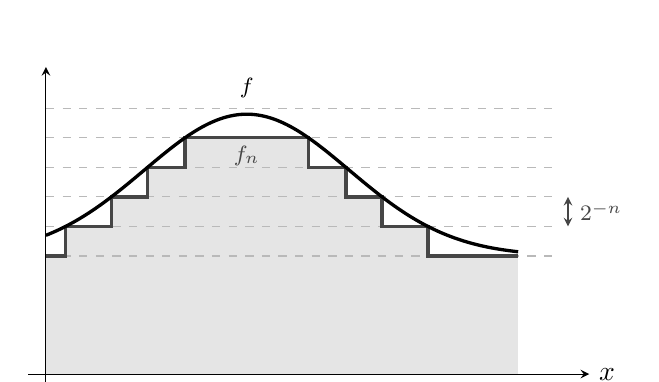
\begin{tikzpicture}[scale=1.5,>=stealth]
    % staircase below f
    \fill[gray!20] (0,0) rectangle (0.166,1.00);
    \fill[gray!20] (0.166,0) rectangle (0.554,1.25);
    \fill[gray!20] (0.554,0) rectangle (0.860,1.50);
    \fill[gray!20] (0.860,0) rectangle (1.177,1.75);
    \fill[gray!20] (1.177,0) rectangle (2.223,2.00);
    \fill[gray!20] (2.223,0) rectangle (2.540,1.75);
    \fill[gray!20] (2.540,0) rectangle (2.846,1.50);
    \fill[gray!20] (2.846,0) rectangle (3.234,1.25);
    \fill[gray!20] (3.234,0) rectangle (4.0,1.00);
    \draw[gray!55,dashed] (0,1.00) -- (4.3,1.00);
    \draw[gray!55,dashed] (0,1.25) -- (4.3,1.25);
    \draw[gray!55,dashed] (0,1.50) -- (4.3,1.50);
    \draw[gray!55,dashed] (0,1.75) -- (4.3,1.75);
    \draw[gray!55,dashed] (0,2.00) -- (4.3,2.00);
    \draw[gray!55,dashed] (0,2.25) -- (4.3,2.25);
    \draw[very thick,gray!55!black]
      (0,1.00) -- (0.166,1.00) -- (0.166,1.25) -- (0.554,1.25) -- (0.554,1.50)
      -- (0.860,1.50) -- (0.860,1.75) -- (1.177,1.75) -- (1.177,2.00)
      -- (2.223,2.00) -- (2.223,1.75) -- (2.540,1.75) -- (2.540,1.50)
      -- (2.846,1.50) -- (2.846,1.25) -- (3.234,1.25) -- (3.234,1.00)
      -- (4.0,1.00);
    \draw[->] (-0.15,0) -- (4.6,0) node[right] {$x$};
    \draw[->] (0,-0.15) -- (0,2.6);
    \draw[very thick,domain=0:4,samples=140,smooth]
      plot (\x,{1+1.2*exp(-(\x-1.7)*(\x-1.7)/1.5)});
    \node at (1.70,2.42) {\footnotesize $f$};
    \node[gray!55!black] at (1.70,1.85) {\footnotesize $f_{n}$};
    \draw[<->,gray!55!black] (4.42,1.25) -- (4.42,1.50);
    \node[right,gray!55!black] at (4.44,1.375) {\footnotesize $2^{-n}$};
  \end{tikzpicture}
\end{figure}

\medskip
The staircase takes, at each point, the largest multiple of $2^{-n}$ below $f$; every
halving of the mesh inserts a new level between two old ones, so the staircase can
only rise, and it rises to $f$. The picture also explains the cut-off at $2^{n}$: a
fonction étagée takes finitely many values and cannot follow $f$ up to $+\infty$, so
the construction truncates and lets the truncation level escape with $n$.

\subsection{Linéarité}

\begin{theorem}[Linéarité]
  Soit $f$ et $g$ des fonctions mesurables de $\Omega$ vers $\bar{\reals}$ dont les
  intégrales sont bien définies. On a :
  \[
    \forall \alpha \in \reals, \qquad
    \int \alpha f \, d\mu = \alpha \int f \, d\mu ,
  \]
  et
  \[
    \int (f + g) \, d\mu = \int f \, d\mu + \int g \, d\mu ,
  \]
  cette dernière égalité étant satisfaite dès que les fonctions $f$ et $g$ sont
  positives ou que l'une d'entre elles est intégrable.
\end{theorem}

\begin{proof}
  On montre successivement les deux propriétés, each by the same ladder: étagée
  positive, then mesurable positive by convergence monotone, then arbitrary sign by
  splitting into positive and negative parts.\\

  \textbf{Homogeneity.} Soit $\alpha \geq 0$. Si $f = \sum_{i=1}^{n} \alpha_{i}
  \indic_{A_{i}}$ est étagée positive, où les ensembles $A_{1},\ldots,A_{n}$ forment
  une partition de $\Omega$, la fonction $\alpha f$ est étagée positive, de sorte
  que $\int \alpha f \, d\mu = \sum_{i} \alpha \alpha_{i} \mu(A_{i}) = \alpha \int f
  \, d\mu$. Si la fonction $f$ est mesurable positive, on considère une suite
  croissante de fonctions étagées positives $(f_{n})$ qui tend vers $f$. Alors
  $(\alpha f_{n})$ est une suite croissante de fonctions étagées positives qui tend
  vers $\alpha f$, and the lemme de convergence monotone gives
  \[
    \int \alpha f \, d\mu = \lim_{n} \uparrow \int \alpha f_{n} \, d\mu
    = \alpha \lim_{n} \uparrow \int f_{n} \, d\mu = \alpha \int f \, d\mu .
  \]
  Si $f$ est une fonction mesurable, d'intégrale bien définie, on applique le
  résultat précédent aux fonctions $(\alpha f)^{+} = \alpha f^{+}$ et $(\alpha
  f)^{-} = \alpha f^{-}$; negative $\alpha$ then follows from the sign-reversal
  proposition.\\

  \textbf{Additivity.} On considère tout d'abord le cas où les fonctions $f$ et $g$
  sont étagées positives. On écrit :
  \[
    f = \sum_{i=1}^{n} \alpha_{i} \indic_{A_{i}}
    \qquad \text{and} \qquad
    g = \sum_{j=1}^{m} \beta_{j} \indic_{B_{j}},
  \]
  où les ensembles $A_{1},\ldots,A_{n}$ et $B_{1},\ldots,B_{m}$ forment des
  partitions de $\Omega$. La fonction $f + g$ est étagée positive, avec :
  \[
    f + g = \sum_{i=1}^{n} \sum_{j=1}^{m} (\alpha_{i} + \beta_{j})
      \indic_{A_{i} \intersect B_{j}} ,
  \]
  and therefore, on obtient :
  \begin{align*}
    \int (f+g) \, d\mu
      &= \sum_{i=1}^{n} \sum_{j=1}^{m} (\alpha_{i} + \beta_{j})
         \mu(A_{i} \intersect B_{j}) \\
      &= \sum_{i=1}^{n} \sum_{j=1}^{m} \alpha_{i} \mu(A_{i} \intersect B_{j})
       + \sum_{i=1}^{n} \sum_{j=1}^{m} \beta_{j} \mu(A_{i} \intersect B_{j}) \\
      &= \sum_{i=1}^{n} \alpha_{i} \mu(A_{i}) + \sum_{j=1}^{m} \beta_{j} \mu(B_{j})
       = \int f \, d\mu + \int g \, d\mu .
  \end{align*}
  Si $f$ et $g$ sont mesurables positives, on considère des suites croissantes de
  fonctions étagées positives $(f_{n})$ et $(g_{n})$ qui tendent respectivement vers
  $f$ et $g$. Alors $(f_{n} + g_{n})$ est une suite croissante de fonctions étagées
  positives qui tend vers $f+g$, and the lemme de convergence monotone gives $\int
  (f+g) \, d\mu = \lim_{n} \uparrow ( \int f_{n} \, d\mu + \int g_{n} \, d\mu ) =
  \int f \, d\mu + \int g \, d\mu$.

  Finally, si $f$ ou $g$ est intégrable,
  \[
    \int (f+g)^{+} \, d\mu \leq \int (f^{+} + g^{+}) \, d\mu
    = \int f^{+} \, d\mu + \int g^{+} \, d\mu < \infty
  \]
  ou
  \[
    \int (f+g)^{-} \, d\mu \leq \int (f^{-} + g^{-}) \, d\mu
    = \int f^{-} \, d\mu + \int g^{-} \, d\mu < \infty ,
  \]
  l'intégrale de $f+g$ est donc bien définie. Comme :
  \[
    f + g = (f+g)^{+} - (f+g)^{-} = f^{+} - f^{-} + g^{+} - g^{-}
  \]
  on a :
  \[
    (f+g)^{+} + f^{-} + g^{-} = (f+g)^{-} + f^{+} + g^{+} ,
  \]
  ces fonctions étant positives, the positive case applies to this identity:
  \[
    \int (f+g)^{+} \, d\mu + \int f^{-} \, d\mu + \int g^{-} \, d\mu
    = \int (f+g)^{-} \, d\mu + \int f^{+} \, d\mu + \int g^{+} \, d\mu ,
  \]
  and rearranging gives $\int (f+g) \, d\mu = \int f \, d\mu + \int g \, d\mu$.
\end{proof}

\begin{remark}[Rearranging into positive parts, and why]
  The last step is the only subtle one. One cannot simply subtract $\int f^{-}$ from
  both sides of an equality between possibly infinite quantities; the rearrangement
  into an identity between \emph{positive} functions is what allows the additive case
  already proved to be applied, and the hypothesis that one of $f$, $g$ is integrable
  is what guarantees that the terms being moved are finite. Drop that hypothesis and
  the statement fails: with $f = \indic_{\reals_{+}}$ and $g = -\indic_{\reals_{+}}$
  the left-hand side is $0$ while the right-hand side is $\infty - \infty$.
\end{remark}

\begin{remark}[The three-stage method]
  The proof just given is the pattern of the whole chapter. A statement about the
  integral is proved first for fonctions étagées positives, where it is a finite
  sum; then for positive mesurable functions, by taking an increasing sequence of
  fonctions étagées and applying the lemme de convergence monotone on each side; then
  for mesurable functions of arbitrary sign, by applying the positive case to $f^{+}$
  and to $f^{-}$ and subtracting, which needs one of the two to be finite. Every
  proof below that begins ``by the three-stage method'' is this argument, and only
  its first stage is ever written out.
\end{remark}

\begin{remark}[The order of the chapter is not circular]
  It looks as though linearity has just been proved using convergence monotone, while
  convergence monotone is stated as a theorem only two subsections below. It is not
  circular, and the point is worth stating once, being the single most confusing
  thing in this chapter. What linearity uses is the \emph{lemma} form: an
  \emph{everywhere} increasing sequence of positive mesurable functions with
  everywhere pointwise limit. That lemma was proved directly from the definition of
  the integral as a supremum over fonctions étagées, using only monotonicity and
  continuity from below of the mesure, and no linearity whatsoever. The
  \emph{theorem} form below weakens the hypothesis to convergence \textit{presque
  partout}, and its proof restricts to the set where convergence holds and invokes
  the lemma there --- and that restriction is where linearity and the results on
  ensembles négligeables are needed. The dependency runs lemma $\to$ linearity $\to$
  ensembles négligeables $\to$ theorem, with no cycle, and these notes keep that
  order.
\end{remark}

\begin{corollary}[L'intégrabilité se lit sur le module]
  Une fonction mesurable $f$ est intégrable si et seulement si $\int |f| \, d\mu <
  \infty$.
\end{corollary}

\begin{proof}
  Comme $|f| = f^{+} + f^{-}$, on a par linéarité de l'intégrale, in the positive
  case :
  \[
    \int |f| \, d\mu = \int f^{+} \, d\mu + \int f^{-} \, d\mu ,
  \]
  qui est finie si et seulement si $\int f^{+} \, d\mu < \infty$ et $\int f^{-} \,
  d\mu < \infty$, that is, if and only if $f$ is integrable.
\end{proof}

\begin{corollary}[Additivité dénombrable de l'intégrale]
  Pour toute suite de fonctions mesurables positives $(f_{n})_{n \geq 1}$,
  \[
    \sum_{n \geq 1} \int f_{n} \, d\mu = \int \left( \sum_{n \geq 1} f_{n} \right)
      d\mu .
  \]
\end{corollary}

\begin{proof}
  La suite $\left( \sum_{n=1}^{k} f_{n} \right)_{k \geq 1}$ (the partial sums) est
  une suite croissante de fonctions mesurables positives qui tend vers $f = \sum_{n
  \geq 1} f_{n}$, so the lemme de convergence monotone gives
  \[
    \lim_{k} \uparrow \int \sum_{n=1}^{k} f_{n} \, d\mu = \int f \, d\mu ,
  \]
  while, par ailleurs, la linéarité de l'intégrale implique que
  \[
    \lim_{k} \uparrow \int \sum_{n=1}^{k} f_{n} \, d\mu
    = \lim_{k} \uparrow \sum_{n=1}^{k} \int f_{n} \, d\mu
    = \sum_{n \geq 1} \int f_{n} \, d\mu . \qedhere
  \]
\end{proof}

\begin{remark}[Positivity is the whole hypothesis]
  Nothing is assumed about convergence: both sides may be $+\infty$, and the corollary
  asserts that they are infinite together. This is the interchange of a sum and an
  integral that costs nothing; it is used below to prove that a mesure à densité is a
  mesure, and again inside the construction of the mesure produit. Without
  positivity the interchange needs domination.
\end{remark}

\subsection{Ensembles négligeables}

On rappelle qu'un ensemble $A \in \mathcal{F}$ est dit négligeable si $\mu(A) = 0$,
as in the previous chapter.

\begin{prop}[Intégrale sur un ensemble négligeable]
  Soit $f : \Omega \to \reals$ une fonction mesurable et $A$ un ensemble négligeable.
  Alors
  \[
    \int_{A} f \, d\mu = 0 .
  \]
\end{prop}

\begin{proof}
  By the three-stage method. Si $f = \sum_{i=1}^{n} \alpha_{i} \indic_{A_{i}}$ est
  étagée positive, alors la fonction $f \indic_{A} = \sum_{i=1}^{n} \alpha_{i}
  \indic_{A_{i} \intersect A}$ est elle-même étagée positive. On en déduit :
  \[
    \int_{A} f \, d\mu = \sum_{i=1}^{n} \alpha_{i} \mu(A_{i} \intersect A)
    \leq \sum_{i=1}^{n} \alpha_{i} \mu(A) = 0 .
  \]
  The two remaining stages use $(f \indic_{A})^{+} = f^{+} \indic_{A}$ and $(f
  \indic_{A})^{-} = f^{-} \indic_{A}$.
\end{proof}

On rappelle qu'une propriété est vraie ``presque partout'' (ce que l'on note p.p.) si
sa négation correspond à un ensemble négligeable, and that the mesure it refers to is
always the one the integral is taken against.

\begin{theorem}[L'intégrale ne voit pas les ensembles négligeables]
  Soit $f, g : \Omega \to \reals$ des fonctions mesurables. Alors
  \begin{enumerate}
    \item $f = 0$ p.p. implique $\int f \, d\mu = 0$ ;
    \item $f = g$ p.p. implique $\int f \, d\mu = \int g \, d\mu$ dès que l'une de
      ces intégrales existe ;
    \item $f \geq 0$ p.p. implique $\int f \, d\mu \geq 0$ ; si de plus $\int f \,
      d\mu = 0$ alors $f = 0$ p.p. ;
    \item $f \leq g$ p.p. implique $\int f \, d\mu \leq \int g \, d\mu$ dès que ces
      intégrales existent ; si de plus $\int f \, d\mu = \int g \, d\mu < \infty$
      alors $f = g$ p.p.
  \end{enumerate}
\end{theorem}

\begin{proof}
  \textbf{1.} L'ensemble $A = \{f \neq 0\}$ est négligeable. Comme $f = f
  \indic_{A}$, on a par la proposition précédente $\int f \, d\mu = \int_{A} f \,
  d\mu = 0$.\\

  \textbf{2.} Si $f, g$ sont positives, on note $A = \{f = g\}$, whose complement is
  négligeable. Comme $f = f \indic_{A} + f \indic_{A^{c}}$, and likewise for $g$, on
  a par linéarité et par la proposition précédente $\int f \, d\mu = \int f
  \indic_{A} \, d\mu = \int g \indic_{A} \, d\mu = \int g \, d\mu$. In general $f^{+}
  = g^{+}$ p.p. et $f^{-} = g^{-}$ p.p., so the positive case applies to each; if
  one of the two integrals is well defined, so is the other, and they are equal.\\

  \textbf{3.} On définit $A = \{f \geq 0\}$. Comme $f = f \indic_{A}$ p.p., on a par
  le résultat précédent $\int f \, d\mu \geq 0$. Si de plus $\int f \, d\mu = 0$, on
  définit $A_{n} = \{f \geq \frac{1}{n}\}$. Comme $f \indic_{A_{n}} \leq f
  \indic_{A}$,
  \[
    \int f \, d\mu \geq \int f \indic_{A_{n}} \, d\mu
    \geq \frac{1}{n} \mu(A_{n}) ,
  \]
  on a donc $\mu(A_{n}) = 0$ pour tout $n$, et comme $A_{n} \uparrow \{f > 0\}$,
  continuity from below gives $\mu(\{f > 0\}) = 0$. On en déduit que $f = 0$ p.p.\\

  \textbf{4.} Soit $A = \{f \leq g\}$, whose complement is négligeable. Comme $f
  \indic_{A} \leq g \indic_{A}$, on a $\int f \, d\mu \leq \int g \, d\mu$ by the
  second point. Si de plus $\int f \, d\mu = \int g \, d\mu < \infty$, alors $g - f
  \geq 0$ p.p. avec $\int (g-f) \, d\mu = 0$, ce qui implique $f = g$ p.p. d'après le
  résultat précédent.
\end{proof}

\begin{remark}[Finiteness in the last statement]
  The finiteness $\int f \, d\mu = \int g \, d\mu < \infty$ in the fourth point is
  not decoration. It is what makes $\int (g-f) \, d\mu = 0$ legitimate: subtracting
  two infinite integrals says nothing. Take $f = \indic_{\reals_{+}}$ and $g =
  \indic_{\reals}$ against $\lambda$. Both integrals are defined and equal to
  $+\infty$, and $f \leq g$ everywhere, yet $f$ and $g$ differ on the whole of
  $]-\infty,0[$, which is very far from négligeable. Equal infinite integrals say
  nothing about the two functions; only equal finite ones do. The same remark applies
  to the equality case of the third point, where the hypothesis is the value $0$,
  which is finite by construction.
\end{remark}

\begin{theorem}[Une fonction intégrable est p.p. finie]
  Toute fonction intégrable est p.p. finie.
\end{theorem}

\begin{proof}
  Soit $f$ une fonction positive intégrable. Notons $A = \{f = +\infty\}$. Pour tout
  $n \geq 1$, $f \geq f_{n}$ avec $f_{n} = n \indic_{A}$. On en déduit :
  \[
    \int f \, d\mu \geq \int f_{n} \, d\mu = n \mu(A) .
  \]
  Si $\mu(A) > 0$ alors, en faisant tendre $n \to +\infty$, on obtient $\int f \,
  d\mu = +\infty$, une contradiction. L'ensemble $A$ est donc négligeable, ce qui
  signifie que $f$ est p.p. finie. Si $f$ est intégrable (of arbitrary sign), alors
  $\int f^{+} \, d\mu < \infty$ et $\int f^{-} \, d\mu < \infty$. D'après le
  résultat précédent, $f^{+}$ et $f^{-}$ sont p.p. finies, ce qui veut dire que $f$
  est p.p. finie.
\end{proof}

\subsection{Convergence monotone, convergence dominée}

This is where the intégrale de Lebesgue earns its place. Two theorems give
conditions under which a limit may be taken inside an integral, and a lemma sits
between them providing an inequality that always holds.

\begin{theorem}[Convergence monotone]
  Soit $f$ une fonction mesurable et $(f_{n})_{n \geq 1}$ une suite croissante de
  fonctions mesurables positives qui converge p.p. vers $f$. Alors :
  \[
    \lim_{n} \int f_{n} \, d\mu = \int f \, d\mu .
  \]
\end{theorem}

\begin{proof}
  Soit $A = \{\lim_{n} f_{n} = f\}$ l'ensemble des points où il y a convergence. Its
  complement is négligeable, so by the lemme de convergence monotone applied to the
  sequence $(f_{n} \indic_{A})$, which increases to $f \indic_{A}$ everywhere,
  \[
    \lim_{n} \int f_{n} \, d\mu = \lim_{n} \int f_{n} \indic_{A} \, d\mu
    = \int f \indic_{A} \, d\mu = \int f \, d\mu ,
  \]
  the first and last equalities being the theorem on ensembles négligeables just
  proved.
\end{proof}

\begin{remark}[The theorem is the lemma, plus p.p.]
  The only thing added to the lemma is the tolerance of a négligeable exceptional
  set, and the proof is the restriction to $A$ that the non-circularity remark above
  anticipated. It is the form one actually applies, because hypotheses in practice
  hold only p.p.
\end{remark}

Le théorème de convergence dominée repose sur le résultat suivant.

\begin{lemma}[Lemme de Fatou (\textit{Fatou's lemma})]
  Pour toute suite $(f_{n})_{n \geq 1}$ de fonctions mesurables positives,
  \[
    \int \liminf_{n} f_{n} \, d\mu \leq \liminf_{n} \int f_{n} \, d\mu .
  \]
\end{lemma}

\begin{proof}
  The sequence $( \inf_{k \geq n} f_{k} )_{n \geq 1}$ is increasing and positive with
  limit $\liminf_{n} f_{n}$, so par convergence monotone, $\int \liminf_{n} f_{n} \,
  d\mu = \lim_{n} \int \inf_{k \geq n} f_{k} \, d\mu$. Comme $\inf_{k \geq n} f_{k}
  \leq f_{k}$ pour tout $k \geq n$, monotonicity gives $\int \inf_{k \geq n} f_{k}
  \, d\mu \leq \inf_{k \geq n} \int f_{k} \, d\mu$, et par passage à la limite,
  $\int \liminf_{n} f_{n} \, d\mu \leq \liminf_{n} \int f_{n} \, d\mu$.
\end{proof}

\begin{remark}[Fatou gives an inequality and nothing more]
  Le lemme de Fatou fournit uniquement une inégalité, which can be strict. Appliqué
  aux fonctions $f_{n} = \indic_{[n,+\infty[}$, against the mesure de Lebesgue, on a
  $\liminf_{n} f_{n} = 0$, si bien que
  \[
    \int \liminf_{n} f_{n} \, d\lambda = 0 ,
    \qquad \text{while} \qquad
    \liminf_{n} \int f_{n} \, d\lambda = +\infty .
  \]
  Mass escaping to infinity is lost in the limit but not in the integrals, and the
  inequality records exactly that loss.
\end{remark}

\begin{theorem}[Convergence dominée (\textit{dominated convergence})]
  Soit $f$ une fonction mesurable et $(f_{n})_{n \geq 1}$ une suite de fonctions
  mesurables qui converge p.p. vers $f$. S'il existe une fonction \emph{intégrable}
  $g$ telle que $|f_{n}| \leq g$ pour tout $n \geq 1$, alors la fonction $f$ est
  intégrable et
  \[
    \lim_{n} \int f_{n} \, d\mu = \int f \, d\mu .
  \]
\end{theorem}

\begin{proof}
  Le lemme de Fatou, applied to $(|f_{n}|)$, implique que
  \[
    \int |f| \, d\mu = \int \liminf_{n} |f_{n}| \, d\mu
    \leq \liminf_{n} \int |f_{n}| \, d\mu \leq \int g \, d\mu < \infty ,
  \]
  de sorte que la fonction $f$ est intégrable. Les fonctions $g - f_{n}$ et $g +
  f_{n}$ étant mesurables positives pour tout $n$, le lemme de Fatou, applied to each
  of the two sequences, implique également que :
  \begin{align*}
    \int g \, d\mu - \int f \, d\mu &= \int (g - f) \, d\mu
      \leq \liminf_{n} \int (g - f_{n}) \, d\mu
      = \int g \, d\mu - \limsup_{n} \int f_{n} \, d\mu , \\
    \int g \, d\mu + \int f \, d\mu &= \int (g + f) \, d\mu
      \leq \liminf_{n} \int (g + f_{n}) \, d\mu
      = \int g \, d\mu + \liminf_{n} \int f_{n} \, d\mu .
  \end{align*}
  Since $\int g \, d\mu$ is finite it can be cancelled from both lines, and on tire de
  ces inégalités que
  \[
    \int f \, d\mu \leq \liminf_{n} \int f_{n} \, d\mu
    \leq \limsup_{n} \int f_{n} \, d\mu \leq \int f \, d\mu ,
  \]
  d'où l'on conclut que la suite $\int f_{n} \, d\mu$ converge vers $\int f \,
  d\mu$.
\end{proof}

\begin{remark}[Where the domination is spent]
  The function $g$ is used three times: to make $f$ integrable, to make $g - f_{n}$
  and $g + f_{n}$ positive so that Fatou applies, and --- decisively --- to allow
  $\int g \, d\mu$ to be cancelled from both sides. That cancellation is illegal if
  $\int g \, d\mu = +\infty$, which is why the hypothesis is not that some function
  dominates the sequence but that an \emph{integrable} one does, and one that works
  for every $n$ simultaneously.
\end{remark}

\begin{example}[Domination cannot be dropped]
  Let $f_{n} = n \indic_{]0,1/n[}$ on $\reals$ with the mesure de Lebesgue. For every
  $x$, $f_{n}(x) \to 0$: a fixed $x > 0$ leaves the interval as soon as $n > 1/x$,
  and $f_{n}(x) = 0$ for $x \leq 0$ throughout. Yet
  \[
    \int f_{n} \, d\lambda = n \cdot \frac{1}{n} = 1
    \qquad \text{for every } n, \qquad \text{while} \qquad
    \int \lim_{n} f_{n} \, d\lambda = 0 .
  \]
  The limit and the integral cannot be exchanged. Any function dominating the whole
  sequence is at least the pointwise supremum $\sup_{n} f_{n}$, the staircase equal
  to $k$ on $]\frac{1}{k+1},\frac{1}{k}[$; it therefore exceeds $x \mapsto 1/x - 1$
  on $]0,1[$, whose integral diverges. No integrable dominating function exists ---
  exactly as the theorem requires. Note
  that Fatou's inequality is satisfied, $0 \leq 1$, as it must be.
\end{example}

\begin{figure}[h!]
  \centering
  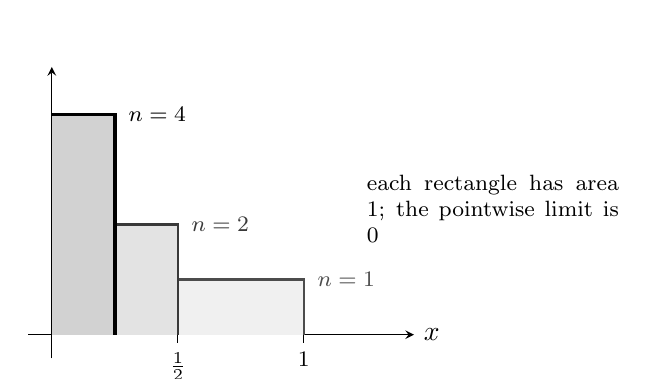
\begin{tikzpicture}[scale=1.0,>=stealth]
    \draw[->] (-0.3,0) -- (4.6,0) node[right] {$x$};
    \draw[->] (0,-0.3) -- (0,3.4);
    % n = 1
    \fill[gray!12] (0,0) rectangle (3.2,0.7);
    \draw[thick,gray!60!black] (0,0.7) -- (3.2,0.7) -- (3.2,0);
    \node[right,gray!60!black] at (3.25,0.7) {\footnotesize $n=1$};
    % n = 2
    \fill[gray!22] (0,0) rectangle (1.6,1.4);
    \draw[thick,gray!45!black] (0,1.4) -- (1.6,1.4) -- (1.6,0);
    \node[right,gray!45!black] at (1.65,1.4) {\footnotesize $n=2$};
    % n = 4
    \fill[gray!35] (0,0) rectangle (0.8,2.8);
    \draw[very thick] (0,2.8) -- (0.8,2.8) -- (0.8,0);
    \node[right] at (0.85,2.8) {\footnotesize $n=4$};
    \draw (3.2,0) -- (3.2,-0.1) node[below] {\footnotesize $1$};
    \draw (1.6,0) -- (1.6,-0.1) node[below] {\footnotesize $\frac{1}{2}$};
    \node at (5.6,1.6) {\parbox{3.2cm}{\footnotesize each rectangle has area
      $1$; the pointwise limit is $0$}};
  \end{tikzpicture}
\end{figure}

\medskip
The picture is the whole counter-example: a rectangle of area $1$ that becomes
taller and narrower without ever losing mass, while at every fixed $x$ it eventually
disappears. Mass escapes upwards here, as it escaped sideways in the Fatou remark,
and an integrable dominating function is precisely a ceiling that forbids both.

\subsection{Lien avec l'intégrale de Riemann}

Nous montrons ici que l'intégrale de Lebesgue généralise l'intégrale de Riemann. On
se donne un intervalle $[a,b]$ de $\reals$ avec $a < b$.

\begin{definition}[Fonction en escalier (\textit{step function})]
  Une fonction $f : [a,b] \to \reals$ est dite \textbf{en escalier} s'il existe une
  subdivision $a = x_{0} < x_{1} < \ldots < x_{n} = b$ de l'intervalle $[a,b]$ telle
  que $f$ est constante sur chaque intervalle $]x_{0},x_{1}[, \ldots,
  ]x_{n-1},x_{n}[$.
\end{definition}

L'intégrale de Riemann d'une fonction en escalier $f$ est définie par :
\[
  \int_{a}^{b} f(x) \, dx = \sum_{i=0}^{n-1} \alpha_{i} (x_{i+1} - x_{i}) ,
\]
où $\alpha_{0},\ldots,\alpha_{n-1}$ sont les valeurs prises par $f$ sur les
intervalles respectifs $]x_{0},x_{1}[, \ldots, ]x_{n-1},x_{n}[$. La fonction $f$
étant étagée in the sense of this chapter, on vérifie aisément que c'est également
l'intégrale de Lebesgue par rapport à la mesure de Lebesgue :
\[
  \int_{[a,b]} f \, d\lambda = \sum_{i=0}^{n-1} \alpha_{i}
    \lambda(]x_{i},x_{i+1}[) = \int_{a}^{b} f(x) \, dx .
\]
A fonction en escalier is the elementary brick of the Riemann theory exactly as a
fonction étagée is of the Lebesgue theory; the difference is that a fonction en
escalier is constant on \emph{intervals} while a fonction étagée is constant on
arbitrary mesurable sets, and that single relaxation is the whole gap between the
two theories.

\begin{definition}[Intégrale de Riemann (\textit{Riemann integral})]
  Une fonction bornée $f : [a,b] \to \reals$ est \textbf{intégrable au sens de
  Riemann} (\textit{Riemann-integrable}) si :
  \[
    \sup \left\{ \int_{a}^{b} g(x) \, dx : g \leq f, \; g \text{ a step function}
    \right\}
    = \inf \left\{ \int_{a}^{b} h(x) \, dx : f \leq h, \; h \text{ a step function}
    \right\} ,
  \]
  cette valeur étant son intégrale, notée $\int_{a}^{b} f(x) \, dx$.
\end{definition}

\begin{theorem}[Intégrable au sens de Riemann implique intégrable au sens de Lebesgue]
  Une fonction $f : [a,b] \to \reals$ intégrable au sens de Riemann a une intégrale
  par rapport à la mesure de Lebesgue et les deux intégrales coïncident :
  \[
    \int_{a}^{b} f(x) \, dx = \int_{[a,b]} f \, d\lambda .
  \]
\end{theorem}

\begin{proof}
  Soit $(g_{n})_{n \geq 1}$ une suite croissante de fonctions en escalier telle que
  $g_{n} \leq f$ pour tout $n$ et :
  \[
    \lim_{n} \int_{a}^{b} g_{n}(x) \, dx = \int_{a}^{b} f(x) \, dx ,
  \]
  et de même, soit $(h_{n})_{n \geq 1}$ une suite décroissante de fonctions en
  escalier telle que $h_{n} \geq f$ pour tout $n$ et :
  \[
    \lim_{n} \int_{a}^{b} h_{n}(x) \, dx = \int_{a}^{b} f(x) \, dx ;
  \]
  both exist by the definition of a fonction intégrable au sens de Riemann, replacing
  a maximising sequence by the running maximum of its terms in the first case and
  the running minimum in the second. Les limites respectives $g$ et $h$ de ces suites
  sont mesurables et bornées, $f$ being bounded, de sorte que, par convergence
  dominée --- the constant bound being integrable on the bounded interval $[a,b]$
  --- both limits of intégrales de Riemann are intégrales de Lebesgue. On a donc :
  \[
    \int_{[a,b]} g \, d\lambda = \int_{a}^{b} f(x) \, dx
    = \int_{[a,b]} h \, d\lambda .
  \]
  Comme $g \leq f \leq h$, the equality case in the theorem on ensembles négligeables
  gives $g = h$ p.p., et donc $g = f = h$ p.p., ce qui implique $\int_{a}^{b} f(x) \,
  dx = \int_{[a,b]} f \, d\lambda$.
\end{proof}

\begin{remark}[Which tribu the Riemann theory really uses]
  Le théorème suggère que toute fonction intégrable au sens de Riemann est mesurable
  pour la tribu de Borel. Ce n'est pas le cas. Elle est mesurable par rapport à la
  \textbf{tribu de Lebesgue} (\textit{Lebesgue $\sigma$-algebra}), définie comme la
  tribu de Borel complétée de tous les ensembles négligeables pour la mesure de
  Lebesgue (ensembles mesurables négligeables et leurs sous-ensembles). Ce détail
  technique ne change rien en pratique, l'intégrale de Lebesgue étant définie de la
  même manière sur la tribu complétée; what the proof above shows is that $f$ agrees
  p.p. with the Borel function $g$.
\end{remark}

Il reste à étendre le résultat aux intégrales impropres. Soit $a, b \in \bar{\reals}$.
Pour toute fonction $f$ localement intégrable au sens de Riemann sur $]a,b[$
(c'est-à-dire dont l'intégrale de Riemann est définie sur tout compact de $]a,b[$),
on définit l'intégrale de Riemann comme la limite lorsqu'elle existe des intégrales
\[
  \int_{a_{n}}^{b_{n}} f(x) \, dx
\]
pour toutes suites $(a_{n})_{n \geq 1}$ et $(b_{n})_{n \geq 1}$ respectivement
strictement décroissante et strictement croissante, de limites $a$ et $b$. On note
toujours cette intégrale $\int_{a}^{b} f(x) \, dx$.

\begin{theorem}[Intégrale de Riemann impropre d'une fonction intégrable]
  Soit $a, b \in \bar{\reals}$ et $f$ une fonction localement intégrable au sens de
  Riemann sur $]a,b[$, avec
  \[
    \int_{a}^{b} |f(x)| \, dx < \infty .
  \]
  Alors :
  \[
    \int_{a}^{b} f(x) \, dx = \int_{[a,b]} f \, d\lambda .
  \]
\end{theorem}

\begin{proof}
  Soit $(a_{n})$ et $(b_{n})$ des suites as above. Par le théorème précédent,
  $\int_{a_{n}}^{b_{n}} |f(x)| \, dx = \int_{[a_{n},b_{n}]} |f| \, d\lambda$ pour
  tout $n$. The functions $|f| \indic_{[a_{n},b_{n}]}$ increase to $|f|
  \indic_{[a,b]}$, so par convergence monotone,
  \[
    \int_{[a,b]} |f| \, d\lambda = \lim_{n} \int_{a_{n}}^{b_{n}} |f(x)| \, dx
    = \int_{a}^{b} |f(x)| \, dx < \infty ,
  \]
  which says that $f$ is Lebesgue-integrable on $[a,b]$. The functions $f
  \indic_{[a_{n},b_{n}]}$ are then dominated by the integrable $|f| \indic_{[a,b]}$
  and converge pointwise to $f \indic_{[a,b]}$, so par convergence dominée, on en
  déduit que $\int_{a}^{b} f(x) \, dx = \int_{[a,b]} f \, d\lambda$.
\end{proof}

\begin{remark}[The hypothesis is absolute integrability, and it is the point]
  Le théorème exige que la fonction soit intégrable, that is $\int_{a}^{b} |f(x)| \,
  dx < \infty$, and not merely that it have a convergent improper integral. Ainsi
  l'intégrale impropre
  \[
    \int_{-\infty}^{+\infty} \frac{\sin x}{x} \, dx
  \]
  est définie au sens de Riemann --- the positive and negative humps cancel in the
  limit, and the value is $\pi$ --- mais pas au sens de Lebesgue, since $\int |\sin
  x / x| \, dx = +\infty$ and the Lebesgue definition subtracts two infinite parts.
  This is the one place where the Riemann theory reaches something the Lebesgue
  theory does not, and the reason is structural: the intégrale de Lebesgue is
  absolute by construction, since it is built from $f^{+}$ and $f^{-}$ separately,
  while an intégrale de Riemann impropre is a limit of symmetric truncations and can
  exploit cancellation.
\end{remark}

\begin{remark}[The converse fails in the other direction too]
  Not every Lebesgue-integrable function is intégrable au sens de Riemann. The
  function $\indic_{\mathbb{Q}}$ on $[0,1]$ has intégrale de Lebesgue $0$, while
  every fonction en escalier below it is $\leq 0$ and every fonction en escalier
  above it is $\geq 1$ on each subinterval, so the lower Riemann sums are $\leq 0$,
  the upper ones $\geq 1$, and the two do not meet. Taken with the previous remark,
  the picture is: the two classes of functions overlap but neither contains the
  other, and where they overlap the two integrals agree.
\end{remark}

Comme l'intégrale de Riemann correspond à une intégrale par rapport à la mesure de
Lebesgue, on utilisera les notations
\[
  \int_{a}^{b} f(x) \, dx
  \qquad \text{and} \qquad
  \int_{[a,b]} f \, d\lambda
\]
indifféremment. Les résultats classiques de l'intégrale comme le théorème fondamental de l'analyse
ou l'intégration par parties s'appliquent à l'intégrale de Lebesgue, par rapport à
la mesure de Lebesgue. Tous ces résultats s'étendent aux fonctions de $n$ variables,
sur l'ensemble $\reals^{n}$ muni de la tribu de Borel.

\subsection{Mesures discrètes}

The integral has been defined against an arbitrary mesure. It is time to see what it
becomes for the two mesures the previous chapter singled out. Against the mesure de
Lebesgue it is the classical integral, as the preceding subsection showed. Nous
allons maintenant caractériser l'intégrale de Lebesgue par rapport à une mesure
discrète: it is a sum --- which is what makes chapter 1, where probabilities were
sums over a countable set, a special case of the theory being built here rather than
a separate subject. The bridge is the following pair of results.

\begin{prop}[Mesure somme]
  Soit $(\mu_{i})_{i \in I}$ une famille de mesures sur $(\Omega,\mathcal{F})$.
  L'intégrale d'une fonction mesurable $f : \Omega \to \bar{\reals}$ par rapport à la
  \textbf{mesure somme} (\textit{sum measure}) $\mu = \sum_{i \in I} \mu_{i}$ est
  donnée par
  \[
    \int f \, d\mu = \sum_{i \in I} \int f \, d\mu_{i} ,
  \]
  si cette intégrale est bien définie, c'est-à-dire si :
  \[
    \sum_{i \in I} \int f^{+} \, d\mu_{i} < \infty
    \qquad \text{or} \qquad
    \sum_{i \in I} \int f^{-} \, d\mu_{i} < \infty .
  \]
\end{prop}

\begin{proof}
  By the three-stage method. Si $f = \sum_{j=1}^{n} \alpha_{j} \indic_{A_{j}}$ est
  une fonction étagée positive, alors
  \[
    \int f \, d\mu = \sum_{j=1}^{n} \alpha_{j} \sum_{i \in I} \mu_{i}(A_{j})
    = \sum_{i \in I} \sum_{j=1}^{n} \alpha_{j} \mu_{i}(A_{j})
    = \sum_{i \in I} \int f \, d\mu_{i} ,
  \]
  the interchange of the two sums being legitimate because all the terms are
  positive. The second stage applies the lemme de convergence monotone once to $\mu$
  and once to each $\mu_{i}$, the interchange of the limit and the sum over $I$ being
  again a matter of positive terms.
\end{proof}

L'archétype des mesures discrètes est la mesure de Dirac.

\begin{prop}[Mesure de Dirac]
  Soit $\delta_{a}$ la mesure de Dirac en $a \in \Omega$. Toute fonction mesurable
  $f : \Omega \to \bar{\reals}$ a pour intégrale :
  \[
    \int f \, d\delta_{a} = f(a) .
  \]
\end{prop}

\begin{proof}
  By the three-stage method. Si $f = \sum_{i=1}^{n} \alpha_{i} \indic_{A_{i}}$ est
  une fonction étagée positive, alors $\int f \, d\delta_{a} = \sum_{i} \alpha_{i}
  \indic_{A_{i}}(a) = f(a)$; the second stage gives $\lim_{n} f_{n}(a) = f(a)$, and
  the third $f^{+}(a) - f^{-}(a) = f(a)$.
\end{proof}

On montre de la même manière que pour toute mesure $\mu = \alpha \delta_{a}$ avec
$\alpha > 0$ et $a \in \Omega$, $\int f \, d\mu = \alpha f(a)$. Combining this with
the mesure somme, on obtient l'intégrale d'une fonction mesurable par rapport à toute
mesure discrète
\[
  \mu = \sum_{i \in I} \alpha_{i} \delta_{a_{i}} ,
\]
où $I$ est un ensemble au plus dénombrable et $\alpha_{i} > 0$, $a_{i} \in \Omega$
pour tout $i \in I$.

\begin{theorem}[L'intégrale par rapport à une mesure discrète est une somme]
  Toute fonction mesurable $f : \Omega \to \bar{\reals}$ a pour intégrale :
  \[
    \int f \, d\mu = \sum_{i \in I} \alpha_{i} f(a_{i})
  \]
  dès que
  \[
    \sum_{i \in I} \alpha_{i} f^{+}(a_{i}) < \infty
    \qquad \text{or} \qquad
    \sum_{i \in I} \alpha_{i} f^{-}(a_{i}) < \infty .
  \]
\end{theorem}

\begin{remark}[The bridge back to the discrete chapter]
  This is the statement that makes the general theory contain the discrete one. A
  discrete probability on a countable $\Omega$ is $\prob = \sum_{\omega \in \Omega}
  p(\omega) \delta_{\omega}$, and the theorem reads $\int f \, d\prob = \sum_{\omega}
  p(\omega) f(\omega)$: every espérance computed in chapter 1 as a weighted sum is
  an intégrale de Lebesgue, and every theorem proved below for the intégrale de
  Lebesgue applies verbatim to those sums. In particular the countable additivity
  corollary above is the interchange of two sums, and convergence dominée is the
  interchange of a limit and a series.
\end{remark}

\begin{example}[The mesure de comptage turns the integral into a series]
  Soit $\mu = \sum_{n \in \mathbb{N}} \delta_{n}$ la mesure de comptage de
  $\mathbb{N}$. L'intégrale d'une fonction mesurable $f : \reals \to \bar{\reals}$
  est la série
  \[
    \int f \, d\mu = \sum_{n=0}^{+\infty} f(n)
  \]
  dès que $\sum_{n=0}^{+\infty} f^{+}(n) < \infty$ ou $\sum_{n=0}^{+\infty}
  f^{-}(n) < \infty$. For $f(x) = e^{-x}$ this gives
  \[
    \int e^{-x} \, d\mu(x) = \sum_{n \geq 0} e^{-n} = \frac{1}{1 - e^{-1}}
    = \frac{e}{e-1} .
  \]
\end{example}

\begin{example}[A mesure with a discrete part and a continuous part]
  Let $\mu = \delta_{0} + \lambda$ on $\reals$. By the proposition on the mesure
  somme,
  \[
    \int_{\reals_{+}} e^{-x} \, d\mu(x)
    = \int_{\reals_{+}} e^{-x} \, d\delta_{0}(x)
      + \int_{\reals_{+}} e^{-x} \, d\lambda(x)
    = 1 + \int_{0}^{+\infty} e^{-x} \, dx = 2 .
  \]
  Nothing in the theory forbids mixing an atom and a continuous part, and lois of
  this kind appear as soon as a variable aléatoire is truncated.
\end{example}

\subsection{Mesures à densité}

Integration produces new mesures. This subsection says which ones, and when every
mesure of a given kind arises this way.

\begin{theorem}[L'intégrale d'une fonction positive définit une mesure]
  Soit $\nu$ une mesure sur $(\Omega,\mathcal{F})$ et $f$ une fonction mesurable
  positive.
  \begin{enumerate}
    \item La fonction $\mu : \mathcal{F} \to [0,+\infty]$ définie par
      \[
        \forall A \in \mathcal{F}, \qquad \mu(A) = \int_{A} f \, d\nu
      \]
      est une mesure sur $(\Omega,\mathcal{F})$.
    \item Supposons la mesure $\nu$ $\sigma$-finie. S'il existe une autre fonction
      mesurable positive $g$ telle que $\mu(A) = \int_{A} g \, d\nu$ pour tout $A \in
      \mathcal{F}$, alors $f = g$ $\nu$-p.p.
  \end{enumerate}
\end{theorem}

\begin{proof}
  \textbf{1.} On vérifie que $\mu(\emptyset) = 0$ et que pour toute famille au plus
  dénombrable $(A_{i})_{i \in I}$ d'éléments deux-à-deux disjoints,
  $\mu(\bigcup_{i} A_{i}) = \int f \sum_{i} \indic_{A_{i}} \, d\nu = \sum_{i} \int f
  \indic_{A_{i}} \, d\nu = \sum_{i} \mu(A_{i})$, the middle equality being the
  countable additivity corollary, applicable because the functions $f
  \indic_{A_{i}}$ are positive.\\

  \textbf{2.} Puisque la mesure $\nu$ est $\sigma$-finie, il existe une suite
  $(A_{n})_{n \geq 1}$ d'éléments de $\mathcal{F}$ telle que $A_{n} \uparrow \Omega$
  et $\nu(A_{n}) < \infty$ pour tout $n$. Soit $B_{n} = \{g + \frac{1}{n} \leq f \leq
  n\}$. On a
  \[
    \int_{A_{n} \intersect B_{n}} g \, d\nu
    = \int_{A_{n} \intersect B_{n}} f \, d\nu
    \leq n \nu(A_{n} \intersect B_{n}) \leq n \nu(A_{n}) < \infty ,
  \]
  so both integrals are finite and may be subtracted, ce qui implique :
  \[
    \int_{A_{n} \intersect B_{n}} (f - g) \, d\nu = 0 .
  \]
  Par ailleurs, $f - g \geq \frac{1}{n}$ on $B_{n}$, so
  \[
    \int_{A_{n} \intersect B_{n}} (f - g) \, d\nu
    \geq \frac{1}{n} \nu(A_{n} \intersect B_{n}) ,
  \]
  ce qui implique $\nu(A_{n} \intersect B_{n}) = 0$. Comme $A_{n} \intersect B_{n}
  \uparrow \{f > g\}$, continuity from below gives that l'ensemble $\{f > g\}$ est
  négligeable pour $\nu$, ce qui veut dire que $f \leq g$ $\nu$-p.p. Par symétrie,
  l'inégalité inverse est vraie $\nu$-p.p., so $f = g$ $\nu$-p.p.
\end{proof}

\begin{remark}[$\sigma$-finiteness is what makes the densité unique]
  The truncation $\{g + \frac{1}{n} \leq f \leq n\}$ intersected with $A_{n}$ exists
  only to make an integral finite so that a subtraction is legal, and the sets
  $A_{n}$ come from $\sigma$-finiteness. Without it uniqueness fails: on
  $(\reals,\mathcal{B}(\reals))$ with $\nu$ the mesure assigning $0$ to $\emptyset$
  and $+\infty$ to every non-empty set, the constant functions $1$ and $2$ define the
  same $\mu$ and differ everywhere. L'énoncé du théorème implique deux mesures, so
  one must also say \emph{which} mesure the p.p. refers to, and here it is $\nu$.
\end{remark}

\begin{definition}[Mesure à densité]
  Soit $\mu$ et $\nu$ deux mesures sur $(\Omega,\mathcal{F})$. On dit que $\mu$
  admet une densité par rapport à $\nu$ s'il existe une fonction mesurable $f :
  \Omega \to \reals_{+}$ telle que :
  \[
    \forall A \in \mathcal{F}, \qquad \mu(A) = \int_{A} f \, d\nu .
  \]
  La fonction $f$ est appelée \textbf{densité} (\textit{density}) de $\mu$ par
  rapport à $\nu$.
\end{definition}

Toute densité est définie à un ensemble négligeable près, au sens où deux mesures de
densités égales presque partout sont égales, which is the theorem on ensembles
négligeables. La réciproque est vraie dès que la mesure $\nu$ est $\sigma$-finie, by
the uniqueness statement just proved. Le fait que
\[
  \forall A \in \mathcal{F}, \qquad \mu(A) = \int_{A} d\mu = \int_{A} f \, d\nu
\]
explique la notation symbolique usuelle
\[
  d\mu = f \, d\nu ,
  \qquad \text{equivalently} \qquad
  f = \frac{d\mu}{d\nu} ,
\]
signifiant que $\mu$ a pour densité $f$ par rapport à $\nu$.

\begin{example}[A densité against the mesure de Lebesgue]
  Soit la fonction définie sur $\reals$ par $f(x) = \frac{1}{1+x^{2}}$. La mesure
  $\mu$ de densité $f$ par rapport à la mesure de Lebesgue est définie par :
  \[
    \forall A \in \mathcal{B}(\reals), \qquad
    \mu(A) = \int_{A} \frac{dx}{1+x^{2}} ,
  \]
  ce qui se note $d\mu = \frac{dx}{1+x^{2}}$. Dividing it by $\pi$ gives the
  \textbf{loi de Cauchy} (\textit{Cauchy distribution}).
\end{example}

\begin{remark}[Densités against a discrete mesure]
  La notion de densité s'applique aux mesures discrètes; there is nothing continuous
  about it. Ainsi la mesure de Dirac $\delta_{0}$ a pour densité la fonction
  $\indic_{\{0\}}$ par rapport à la mesure de comptage $\mu = \sum_{n \geq 0}
  \delta_{n}$, since
  \[
    \forall A \in \mathcal{B}(\reals), \qquad
    \delta_{0}(A) = \indic_{A}(0) = \int_{A} \indic_{\{0\}} \, d\mu .
  \]
  The weights of a discrete loi are a densité just as the densité of a continuous
  loi is.
\end{remark}

By the proposition on ensembles négligeables, tout ensemble négligeable pour la
mesure $\nu$ est également négligeable pour la mesure $\mu$ whenever $\mu$ has a
densité with respect to $\nu$. That property has a name.

\begin{definition}[Absolue continuité]
  Soit $\mu$ et $\nu$ deux mesures sur $(\Omega,\mathcal{F})$. On dit que $\mu$ est
  \textbf{absolument continue} (\textit{absolutely continuous}) par rapport à $\nu$,
  ce que l'on note $\mu \ll \nu$, si
  \[
    \forall A \in \mathcal{F}, \qquad \nu(A) = 0 \implies \mu(A) = 0 .
  \]
\end{definition}

Une mesure ayant une densité par rapport à $\nu$ est absolument continue par rapport
à $\nu$ ; le \textbf{théorème de Radon-Nikodym} (\textit{Radon--Nikodym theorem})
fournit une réciproque. La preuve est omise.

\begin{theorem}[Théorème de Radon-Nikodym]
  Soit $\mu$ et $\nu$ deux mesures $\sigma$-finies telles que $\mu \ll \nu$. Alors
  $\mu$ admet une densité par rapport à $\nu$.
\end{theorem}

\begin{remark}[Both mesures must be $\sigma$-finite]
  With $\nu$ the mesure de comptage on $\reals$, which is not $\sigma$-finie, and
  $\mu = \lambda$, one has $\mu \ll \nu$ --- only the empty set is
  $\nu$-négligeable --- yet $\lambda$ has no densité with respect to $\nu$, since
  such a densité would vanish at every point and give $\lambda(A) = 0$ for every
  $A$. Chapter 4 invokes this theorem to say that a real variable aléatoire has a
  densité exactly when its loi is absolument continue with respect to $\lambda$, and
  chapter 5 again to build densités conditionnelles; both times the
  $\sigma$-finiteness is available and unremarked.
\end{remark}

L'intégrale d'une fonction par rapport à une mesure à densité s'écrit de façon très
naturelle, grâce à l'écriture symbolique.

\begin{theorem}[Intégrale par rapport à une mesure à densité]
  Soit $\mu$ une mesure de densité $f$ par rapport à $\nu$. Pour toute fonction
  mesurable $g : \Omega \to \bar{\reals}$,
  \[
    \int g \, d\mu = \int g f \, d\nu
  \]
  dès que l'une de ces intégrales est bien définie.
\end{theorem}

\begin{proof}
  By the three-stage method. Supposons tout d'abord la fonction $g = \sum_{i=1}^{n}
  \alpha_{i} \indic_{A_{i}}$ étagée positive. Alors
  \[
    \int g \, d\mu = \sum_{i=1}^{n} \alpha_{i} \mu(A_{i})
    = \sum_{i=1}^{n} \alpha_{i} \int \indic_{A_{i}} f \, d\nu = \int g f \, d\nu .
  \]
  The second stage needs the lemme de convergence monotone twice, once for $(g_{n})$
  increasing to $g$ and once for $(g_{n} f)$ increasing to $gf$.
\end{proof}

\begin{example}[Integrating against a mesure with a densité]
  L'intégrale de la fonction $\indic_{\reals_{+}}$ par rapport à la mesure $\mu$ de
  densité $x \mapsto \frac{1}{1+x^{2}}$ par rapport à la mesure de Lebesgue est
  donnée par :
  \[
    \int \indic_{\reals_{+}} \, d\mu = \int_{0}^{+\infty} \frac{dx}{1+x^{2}}
    = \frac{\pi}{2} .
  \]
\end{example}

\begin{example}[An exponential weighting]
  Soit $\mu$ la mesure de densité $x \mapsto e^{-x}$ par rapport à la mesure de
  Lebesgue. Then
  \[
    \int_{\reals_{+}} e^{x/2} \, d\mu(x)
    = \int_{0}^{+\infty} e^{x/2} e^{-x} \, dx
    = \int_{0}^{+\infty} e^{-x/2} \, dx = 2 .
  \]
  The densité is absorbed into the integrand; this is the only computation rule
  there is for such mesures.
\end{example}

\subsection{Théorème de transfert}

Soit $\mu$ une mesure sur $(\Omega,\mathcal{F})$. Soit $(E,\mathcal{E})$ un espace
mesurable. Toute fonction mesurable $\phi : \Omega \to E$ définit une mesure sur
$(E,\mathcal{E})$, appelée la mesure image de $\mu$ par $\phi$ et notée
$\mu_{\phi}$, defined in the previous chapter by $\mu_{\phi}(B) =
\mu(\phi^{-1}(B))$. On s'intéresse à l'intégrale de la fonction $f \circ \phi$ par
rapport à la mesure $\mu$ pour une fonction mesurable $f : E \to \bar{\reals}$.

\begin{figure}[h!]
  \centering
  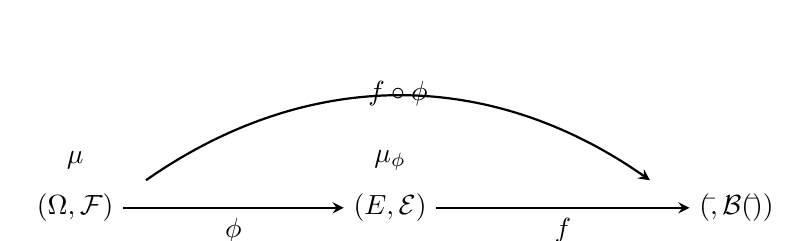
\begin{tikzpicture}[scale=1.0,>=stealth]
    \node (A) at (0,0) {$(\Omega,\mathcal{F})$};
    \node (B) at (4,0) {$(E,\mathcal{E})$};
    \node (C) at (8.4,0) {$(\bar{\reals},\mathcal{B}(\bar{\reals}))$};
    \node at (0,0.6) {$\mu$};
    \node at (4,0.6) {$\mu_{\phi}$};
    \draw[->,thick] (A) -- (B) node[midway,below] {$\phi$};
    \draw[->,thick] (B) -- (C) node[midway,below] {$f$};
    \draw[->,thick] (0.9,0.35) to[out=35,in=145] (7.3,0.35);
    \node at (4.1,1.45) {$f \circ \phi$};
  \end{tikzpicture}
\end{figure}

\medskip

\begin{theorem}[Transfert]
  Soit $f : E \to \bar{\reals}$ une fonction mesurable. On a :
  \[
    \int f \circ \phi \, d\mu = \int f \, d\mu_{\phi}
  \]
  dès que l'une de ces deux intégrales est définie.
\end{theorem}

\begin{proof}
  Supposons la fonction $f$ étagée positive, soit :
  \[
    f = \sum_{i=1}^{n} \alpha_{i} \indic_{B_{i}} ,
  \]
  où $\alpha_{1},\ldots,\alpha_{n}$ sont les valeurs prises par $f$. La fonction $f
  \circ \phi$ est elle-même étagée :
  \[
    f \circ \phi = \sum_{i=1}^{n} \alpha_{i} \indic_{A_{i}} ,
    \qquad A_{i} = \phi^{-1}(B_{i}) ,
  \]
  because $\indic_{B_{i}} \circ \phi = \indic_{\phi^{-1}(B_{i})}$. On obtient :
  \[
    \int f \circ \phi \, d\mu = \sum_{i=1}^{n} \alpha_{i} \mu(A_{i})
    = \sum_{i=1}^{n} \alpha_{i} \mu_{\phi}(B_{i}) = \int f \, d\mu_{\phi} ,
  \]
  the middle equality being nothing but the definition of the mesure image. Si la
  fonction $f$ est mesurable positive, on choisit une suite croissante de fonctions
  étagées positives $(f_{n})$ qui tend vers $f$. La suite $(f_{n} \circ \phi)$ étant
  une suite croissante de fonctions étagées positives qui tend vers $f \circ \phi$,
  the lemme de convergence monotone applied on each side gives
  \[
    \int f \circ \phi \, d\mu = \lim_{n} \uparrow \int f_{n} \circ \phi \, d\mu
    = \lim_{n} \uparrow \int f_{n} \, d\mu_{\phi} = \int f \, d\mu_{\phi} .
  \]
  Enfin, si la fonction $f$ est mesurable (of arbitrary sign), on a $(f \circ
  \phi)^{+} = f^{+} \circ \phi$ et $(f \circ \phi)^{-} = f^{-} \circ \phi$, so by the
  positive case
  \[
    \int (f \circ \phi)^{+} \, d\mu = \int f^{+} \, d\mu_{\phi}
    \qquad \text{and} \qquad
    \int (f \circ \phi)^{-} \, d\mu = \int f^{-} \, d\mu_{\phi} ,
  \]
  ce qui montre l'égalité dès que l'une de ces intégrales est bien définie.
\end{proof}

\begin{remark}[The theorem the rest of the course runs on]
  Read with $\Omega$ an espace de probabilité, $\phi$ a variable aléatoire $X$ and
  $\mu_{\phi}$ its loi $\prob_{X}$, the identity becomes
  \[
    \expec(f(X)) = \int f \, d\prob_{X} .
  \]
  The left-hand side is an integral over an abstract space nobody ever describes; the
  right-hand side is an integral over the value space against an object one can write
  down. That is why the loi is all one ever needs to know about a variable aléatoire,
  and it is why this theorem is used, usually silently, in every computation of
  chapters 4 to 8: to compute an espérance from a loi, to define the fonction
  caractéristique, to identify a loi by testing it against bounded continuous
  functions, and to read an espérance conditionnelle as an integral against a loi
  conditionnelle.
\end{remark}

\subsection{Changement de variable}

Le théorème de transfert permet de changer de variable d'intégration. Considérons
par exemple une fonction $f : \reals \to \bar{\reals}$ mesurable. On souhaite
intégrer la fonction $x \mapsto f(ax+b)$ par rapport à la mesure de Lebesgue, avec
$a \neq 0$. La mesure image de la mesure de Lebesgue par la fonction affine $\phi : x
\mapsto ax+b$ étant la mesure $\frac{\lambda}{|a|}$, le théorème de transfert
s'écrit :
\[
  \int f(ax+b) \, dx = \int f(y) \frac{dy}{|a|}
\]
dès que l'une de ces deux intégrales est définie. On a ainsi procédé au
\textbf{changement de variable} (\textit{change of variable}) de $x$ vers $y =
ax+b$. L'écriture symbolique de ce changement de variable est :
\[
  dy = |a| \, dx
  \qquad \text{or} \qquad
  dx = \frac{dy}{|a|} ,
\]
ce qui revient à dire que la mesure image de $\lambda$ par $\phi$ est
$\frac{\lambda}{|a|}$. On note la présence de la valeur absolue, une mesure étant une
application à valeurs positives: the factor relating two mesures cannot be negative.

Le résultat se généralise à tout difféomorphisme $\phi$. Nous allons voir que la
mesure image de la mesure de Lebesgue est alors une mesure à densité.

\begin{definition}[Difféomorphisme]
  On appelle \textbf{difféomorphisme} une fonction de classe $C^{1}$ bijective, dont
  la réciproque $\phi^{-1}$ est elle-même de classe $C^{1}$.
\end{definition}

On remarque qu'un difféomorphisme est une fonction mesurable (car continue).

\begin{prop}[Changement de variable sur $\reals$]
  Soit $\phi : \reals \to \reals$ un difféomorphisme. Pour toute fonction mesurable
  $f : \reals \to \bar{\reals}$, on a :
  \[
    \int f \circ \phi(x) \, dx
    = \int f(y) \frac{dy}{|\phi'(\phi^{-1}(y))|}
  \]
  dès que l'une de ces deux intégrales est définie.
\end{prop}

\begin{proof}
  La mesure image de la mesure de Lebesgue par $\phi$ vérifie :
  \begin{align*}
    \lambda_{\phi}([a,b]) &= \lambda(\phi^{-1}([a,b])) \\
      &= |\phi^{-1}(b) - \phi^{-1}(a)| \\
      &= \int_{a}^{b} |(\phi^{-1})'(y)| \, dy
       = \int_{a}^{b} \frac{dy}{|\phi'(\phi^{-1}(y))|} ,
  \end{align*}
  où l'on a utilisé le fait que $\phi^{-1}$ est de classe $C^{1}$ et monotone --- so
  that $\phi^{-1}([a,b])$ is the interval with endpoints $\phi^{-1}(a)$ and
  $\phi^{-1}(b)$ --- and then the fundamental theorem of analysis. On en déduit que
  $\lambda_{\phi}$ est la mesure de densité
  \[
    y \mapsto \frac{1}{|\phi'(\phi^{-1}(y))|}
  \]
  par rapport à la mesure de Lebesgue, these two mesures agreeing on the intervals,
  which generate $\mathcal{B}(\reals)$ and are stable par intersection finie. Le
  résultat est une conséquence du théorème de transfert, together with the theorem
  on integration against a mesure à densité.
\end{proof}

L'écriture symbolique du changement de variable $y = \phi(x)$ est :
\[
  dy = |\phi'(x)| \, dx
  \qquad \text{or} \qquad
  dx = \frac{dy}{|\phi'(\phi^{-1}(y))|} .
\]
Comme dans le cas affine, il faut veiller à ne pas oublier la valeur absolue, toute
densité étant une fonction positive.

\begin{remark}[The derivative cannot vanish]
  La dérivée de la fonction $\phi$ ne s'annule pas car $\phi$ est un
  difféomorphisme --- differentiating $\phi^{-1} \circ \phi = \id$ gives
  $(\phi^{-1})'(\phi(x)) \phi'(x) = 1$. C'est d'ailleurs une condition nécessaire et
  suffisante pour qu'une fonction bijective de classe $C^{1}$ soit un
  difféomorphisme (théorème d'inversion globale).
\end{remark}

Le résultat s'étend à tout difféomorphisme $\phi : U \to V$ avec $U$ et $V$ ouverts
de $\reals$, which is what licenses cutting the line into pieces when a map fails to
be a diffeomorphism at isolated points.

\begin{example}[A bijection that is not a diffeomorphism]
  Soit la fonction définie sur $\reals$ par $\phi(x) = x^{3}$. It is a $C^{1}$
  bijection, but cette fonction n'est pas un difféomorphisme puisque sa dérivée
  s'annule en $0$ --- equivalently, $\phi^{-1}(y) = y^{1/3}$ is not differentiable
  at $0$. Pour changer de variable, il faut donc exclure le point $0$ et appliquer
  deux changements de variable successifs, sur les ouverts $]-\infty,0[$ et
  $]0,+\infty[$. Excluding a single point costs nothing, since it is négligeable for
  the mesure de Lebesgue.
\end{example}

Ces résultats s'étendent à des fonctions de $n$ variables. Il faut pour cela
introduire la notion de matrice jacobienne.

\begin{definition}[Matrice jacobienne]
  La \textbf{matrice jacobienne} (\textit{Jacobian matrix}) d'une fonction dérivable
  $\phi : \reals^{n} \to \reals^{n}$ est la matrice des dérivées partielles :
  \[
    \forall x \in \reals^{n}, \qquad
    J_{\phi}(x) = \left( \frac{\partial \phi_{i}}{\partial x_{j}}(x)
      \right)_{1 \leq i,j \leq n} .
  \]
\end{definition}

Le déterminant de la matrice jacobienne s'appelle le jacobien. Pour tout
difféomorphisme $\phi$, la fonction $\phi \circ \phi^{-1}$ est la fonction identité,
de sorte que :
\[
  J_{\phi^{-1}} \times J_{\phi} \circ \phi^{-1} = I
  \qquad \text{and} \qquad
  \det J_{\phi^{-1}} = \frac{1}{(\det J_{\phi}) \circ \phi^{-1}} .
\]
Comme dans le cas des fonctions réelles, une fonction bijective de classe $C^{1}$ est
un difféomorphisme si et seulement si son jacobien ne s'annule pas.

\begin{theorem}[Changement de variable]
  Soit $\phi : \reals^{n} \to \reals^{n}$ un difféomorphisme. Pour toute fonction
  mesurable $f : \reals^{n} \to \bar{\reals}$, on a :
  \[
    \int f \circ \phi(x) \, dx
    = \int \frac{f(y)}{|(\det J_{\phi}) \circ \phi^{-1}(y)|} \, dy
  \]
  dès que l'une de ces deux intégrales est définie.
\end{theorem}

\begin{proof}
  On donne une preuve partielle, dans le cas où $\phi$ est une application affine
  bijective, soit $\phi(x) = Ax + b$ avec $A$ matrice inversible. Le cas général se
  traite par une approximation locale affine de $\phi$. La mesure image de la mesure
  de Lebesgue $\lambda$ par $\phi$ est $\frac{\lambda}{|\det A|}$, a computation
  carried out in the previous chapter for the affine maps of $\reals^{n}$. Comme
  $J_{\phi} = A$, which is constant, on obtient :
  \[
    \lambda_{\phi} = \frac{\lambda}{|\det J_{\phi}|} ,
  \]
  and le résultat est une conséquence du théorème de transfert, together with
  integration against a mesure à densité.
\end{proof}

\begin{figure}[h!]
  \centering
  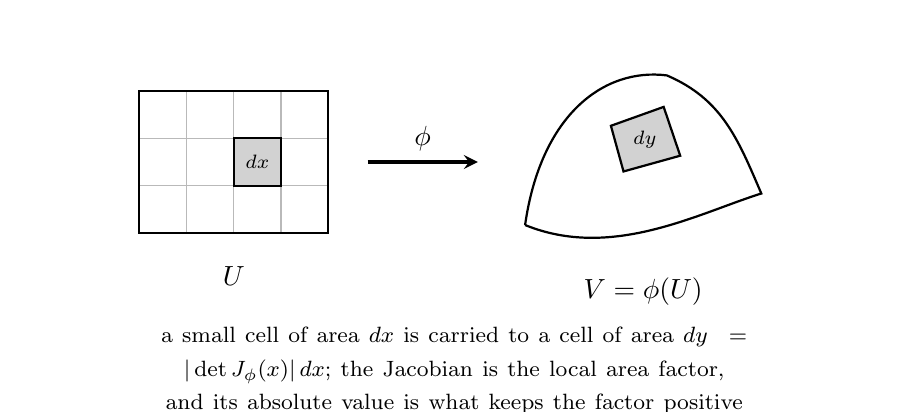
\begin{tikzpicture}[scale=1.0,>=stealth]
    % --- source region with a square grid ---
    \draw[gray!55] (0,0) grid[step=0.6] (2.4,1.8);
    \draw[thick] (0,0) rectangle (2.4,1.8);
    \fill[gray!35] (1.2,0.6) rectangle (1.8,1.2);
    \draw[thick] (1.2,0.6) rectangle (1.8,1.2);
    \node[below] at (1.2,-0.30) {$U$};
    \node at (1.5,0.9) {\scriptsize $dx$};
    % --- the map ---
    \draw[->,very thick] (2.9,0.9) -- (4.3,0.9) node[midway,above] {$\phi$};
    % --- image region, deformed ---
    \draw[thick] (4.9,0.1) .. controls (6.0,-0.35) and (7.1,0.25) .. (7.9,0.5)
      .. controls (7.6,1.2) and (7.4,1.7) .. (6.7,2.0)
      .. controls (5.9,2.1) and (5.1,1.5) .. (4.9,0.1);
    \fill[gray!35] (6.15,0.78) -- (6.87,0.98) -- (6.66,1.60) -- (5.99,1.36) -- cycle;
    \draw[thick] (6.15,0.78) -- (6.87,0.98) -- (6.66,1.60) -- (5.99,1.36) -- cycle;
    \node[below] at (6.4,-0.45) {$V = \phi(U)$};
    \node at (6.42,1.19) {\scriptsize $dy$};
    \node[text width=10.6cm,align=center] at (4.0,-1.75)
      {\footnotesize a small cell of area $dx$ is carried to a cell of area
       $dy = |\det J_{\phi}(x)| \, dx$; the Jacobian is the local area factor,
       and its absolute value is what keeps the factor positive};
  \end{tikzpicture}
  \vspace{0.9cm}
\end{figure}

\medskip
The picture is the content of the theorem. A diffeomorphism deforms a small cell into
a small parallelogram whose area is $|\det J_{\phi}(x)|$ times the original, since
$\phi$ is locally its own derivative; summing over cells turns that local factor
into the densité relating the two mesures. Le résultat s'étend à tout
difféomorphisme $\phi : U \to V$ between open sets of $\reals^{n}$, which is the
form used in practice --- polar coordinates, for instance, are a diffeomorphism from
$]0,+\infty[ \times \, ]0,2\pi[$ onto the plane minus a half-line, and the missing
half-line is négligeable.

\begin{example}[Polar coordinates and the Gaussian integral]
  Let $\phi(r,\theta) = (r\cos\theta, r\sin\theta)$, a diffeomorphism from
  $]0,+\infty[ \times \, ]0,2\pi[$ onto $\reals^{2}$ minus a half-line, with
  $\det J_{\phi}(r,\theta) = r$. For $f(x,y) = e^{-(x^{2}+y^{2})}$,
  \[
    \int_{\reals^{2}} e^{-(x^{2}+y^{2})} \, dx \, dy
    = \int_{0}^{2\pi} \int_{0}^{+\infty} e^{-r^{2}} r \, dr \, d\theta
    = 2\pi \cdot \frac{1}{2} = \pi .
  \]
  The left-hand side is the square of $\int_{-\infty}^{+\infty} e^{-x^{2}} \, dx$ by
  Fubini for positive functions, so that integral equals $\sqrt{\pi}$ --- the
  normalisation behind every densité gaussienne in these notes.
\end{example}

\begin{example}[The volume of an ellipsoid]
  Soit $a,b,c > 0$ et
  \[
    E = \left\{ (x,y,z) \in \reals^{3} :
      \frac{x^{2}}{a^{2}} + \frac{y^{2}}{b^{2}} + \frac{z^{2}}{c^{2}} \leq 1
    \right\} .
  \]
  The linear map $\phi(u,v,w) = (au,bv,cw)$ is a diffeomorphism of $\reals^{3}$
  carrying the unit ball onto $E$, with constant Jacobian $abc$, so
  \[
    \lambda(E) = abc \cdot \lambda(\text{unit ball}) = \frac{4}{3} \pi abc .
  \]
\end{example}

\subsection{Mesure produit}

Soit $\mu$ et $\nu$ des mesures $\sigma$-finies sur les espaces mesurables
respectifs $(E,\mathcal{E})$ et $(F,\mathcal{F})$. On souhaite en déduire une mesure
sur l'espace produit $(E \times F, \mathcal{E} \otimes \mathcal{F})$.

\begin{theorem}[Existence et unicité du produit]
  Il existe une unique mesure $\pi$ sur $(E \times F, \mathcal{E} \otimes
  \mathcal{F})$ telle que :
  \[
    \forall A \in \mathcal{E}, \; \forall B \in \mathcal{F}, \qquad
    \pi(A \times B) = \mu(A) \nu(B) .
  \]
\end{theorem}

\begin{proof}
  \textbf{Uniqueness.} The rectangles $A \times B$ are stable par intersection finie
  and generate $\mathcal{E} \otimes \mathcal{F}$. Les mesures $\mu$ et $\nu$ étant
  $\sigma$-finies, il existe des suites telles que $A_{n} \uparrow E$ et $B_{n}
  \uparrow F$, et $\mu(A_{n}) < \infty$ et $\nu(B_{n}) < \infty$. La suite vérifie
  $A_{n} \times B_{n} \uparrow E \times F$ et $\pi(A_{n} \times B_{n}) = \mu(A_{n})
  \nu(B_{n}) < \infty$. On est donc dans les conditions du théorème d'unicité of the
  previous chapter.\\

  \textbf{Existence.} On définit :
  \[
    \forall C \in \mathcal{E} \otimes \mathcal{F}, \qquad
    \pi(C) = \int \left( \int \indic_{C}(x,y) \, d\nu(y) \right) d\mu(x) .
  \]
  Cette définition n'a de sens que si la fonction $y \mapsto \indic_{C}(x,y)$ est
  mesurable pour tout $x$, et si la fonction $x \mapsto \int \indic_{C}(x,y) \,
  d\nu(y)$ est mesurable. C'est le point technique de la preuve, and it is settled
  in two steps.

  Pour le premier point, the collection of $C$ for which $y \mapsto \indic_{C}(x,y)$
  est mesurable est une tribu. En effet, elle contient l'ensemble $E \times F$ (car
  alors $\indic_{C} = 1$), est stable par passage au complémentaire (en utilisant le
  fait que $\indic_{C^{c}} = 1 - \indic_{C}$) et par intersection dénombrable (car
  $\indic_{\bigcap_{n} C_{n}} = \prod_{n} \indic_{C_{n}}$); and it contains every
  rectangle, because $\indic_{A \times B}(x,y) = \indic_{B}(y)$ for $x \in A$ and $0$
  otherwise. It is therefore the whole of $\mathcal{E} \otimes \mathcal{F}$.

  Pour le second point, on considère une suite telle que $B_{n} \uparrow F$ et
  $\nu(B_{n}) < \infty$; it is enough to treat $x \mapsto \int \indic_{C}(x,y)
  \indic_{B_{n}}(y) \, d\nu(y)$ for each $n$, the general case following by an
  increasing passage to the limit. The collection $\mathcal{M}$ of $C$ for which that
  function is mesurable est une \emph{classe monotone}: it contains $E \times F$;
  for $C \subr D$ in $\mathcal{M}$ the integral over $D \setminus C$ is the
  difference of the two integrals, legitimately because $\nu(B_{n}) < \infty$ makes
  them finite, ce qui montre que $D \setminus C \in \mathcal{M}$; and for $C_{k}
  \uparrow C$ in $\mathcal{M}$, convergence monotone gives $C \in \mathcal{M}$. As
  $\mathcal{M}$ contains the rectangles, which are stable par intersection finie,
  the lemme de classe monotone gives $\mathcal{M} = \mathcal{E} \otimes
  \mathcal{F}$.

  La suite de la preuve est plus aisée. On vérifie que $\pi(\emptyset) = 0$ et que
  pour toute famille au plus dénombrable $(C_{i})_{i \in I}$ d'éléments deux-à-deux
  disjoints,
  \[
    \pi \left( \bigcup_{i \in I} C_{i} \right)
    = \int \left( \int \sum_{i \in I} \indic_{C_{i}}(x,y) \, d\nu(y) \right) d\mu(x)
    = \sum_{i \in I} \pi(C_{i}) ,
  \]
  où les deux inversions somme-intégrale sont justifiées par the countable
  additivity corollary, which applies because the integrands are positive. Il ne
  reste plus qu'à vérifier la propriété annoncée :
  \[
    \pi(A \times B)
    = \int \left( \int \indic_{B}(y) \, d\nu(y) \right) \indic_{A}(x) \, d\mu(x)
    = \mu(A) \nu(B) . \qedhere
  \]
\end{proof}

\begin{definition}[Mesure produit]
  Soit $\mu$ et $\nu$ des mesures $\sigma$-finies sur les espaces mesurables
  respectifs $(E,\mathcal{E})$ et $(F,\mathcal{F})$. On appelle \textbf{mesure
  produit} (\textit{product measure}), que l'on note $\mu \otimes \nu$, l'unique
  mesure sur $(E \times F, \mathcal{E} \otimes \mathcal{F})$ telle que :
  \[
    \forall A \in \mathcal{E}, \; \forall B \in \mathcal{F}, \qquad
    \mu \otimes \nu(A \times B) = \mu(A) \nu(B) .
  \]
\end{definition}

\begin{example}[A mesure on the plane that is not a product]
  La mesure $\mu = \delta_{(0,1)} + \delta_{(1,0)}$ sur
  $(\reals^{2},\mathcal{B}(\reals^{2}))$ n'est pas une mesure produit. Supposons
  $\mu = \mu_{1} \otimes \mu_{2}$. Alors $\mu(\{0\} \times \reals) = \mu_{1}(\{0\})
  \mu_{2}(\reals) = 1$ implique $\mu_{1}(\{0\}) > 0$, and $\mu(\reals \times \{0\}) =
  \mu_{1}(\reals) \mu_{2}(\{0\}) = 1$ implique $\mu_{2}(\{0\}) > 0$. En particulier,
  $\mu(\{(0,0)\}) = \mu_{1}(\{0\}) \mu_{2}(\{0\}) > 0$, alors que $\mu$ puts no mass
  at $(0,0)$. A mesure produit cannot charge two points off the diagonal of a
  rectangle without charging the two remaining corners as well.
\end{example}

\begin{example}[The product of two densités is a densité for the product]
  Soit $\nu_{1}$ et $\nu_{2}$ des mesures $\sigma$-finies sur les espaces
  mesurables $(E_{1},\mathcal{E}_{1})$ et $(E_{2},\mathcal{E}_{2})$. On note
  $\mu_{1}$ et $\mu_{2}$ des mesures de densités $f_{1}$ et $f_{2}$ with respect to
  them. Alors la mesure produit $\mu_{1} \otimes \mu_{2}$ a pour densité $(x_{1},x_{2})
  \mapsto f_{1}(x_{1}) f_{2}(x_{2})$ par rapport à la mesure produit $\nu_{1}
  \otimes \nu_{2}$. On a rectangle $A_{1} \times A_{2}$ the integrand is positive, so
  the integral may be computed one variable at a time --- a case of the
  Fubini--Tonelli theorem below --- and it factorises into $\mu_{1}(A_{1})
  \mu_{2}(A_{2})$. Rectangles determine the mesure produit by the uniqueness just
  proved, so the two mesures coincide.
\end{example}

Le résultat se généralise à un produit d'ordre supérieur. Soit
$\mu_{1},\ldots,\mu_{n}$ des mesures $\sigma$-finies sur les espaces mesurables
respectifs $(E_{1},\mathcal{E}_{1}),\ldots,(E_{n},\mathcal{E}_{n})$.

\begin{theorem}[Produits d'ordre $n$]
  Il existe une unique mesure $\pi$ sur $(E_{1} \times \ldots \times E_{n},
  \mathcal{E}_{1} \otimes \ldots \otimes \mathcal{E}_{n})$ telle que :
  \[
    \forall A_{1} \in \mathcal{E}_{1}, \ldots, \forall A_{n} \in \mathcal{E}_{n},
    \qquad
    \pi(A_{1} \times \ldots \times A_{n}) = \mu_{1}(A_{1}) \ldots \mu_{n}(A_{n}) .
  \]
  On la notera $\mu_{1} \otimes \ldots \otimes \mu_{n}$.
\end{theorem}

\begin{proof}
  La preuve de l'unicité est la même que celle du théorème précédent. On prouve
  l'existence par récurrence sur $n$: si la propriété est vraie au rang $n-1$, the
  two-factor theorem applied to the mesure it produces and to $\mu_{n}$ gives
  $\pi(A_{1} \times \ldots \times A_{n}) = \mu_{1}(A_{1}) \ldots \mu_{n}(A_{n})$.
\end{proof}

\begin{corollary}[Mesure de Lebesgue]
  La mesure de Lebesgue sur $(\reals^{n},\mathcal{B}(\reals^{n}))$ est le produit des
  mesures de Lebesgue sur $(\reals,\mathcal{B}(\reals))$.
\end{corollary}

\begin{proof}
  Ces mesures sont égales sur les pavés $[a_{1},b_{1}] \times \ldots \times
  [a_{n},b_{n}]$, qui engendrent la tribu de Borel de $\reals^{n}$ et sont stables
  par intersection finie. Comme $\reals^{n}$ peut être couvert par une réunion
  croissante de pavés of finite mesure, on est dans les conditions du théorème
  d'unicité of the previous chapter, prouvant l'égalité de ces mesures.
\end{proof}

\begin{remark}[Why $\sigma$-finiteness is in the definition]
  The mesure produit is defined only when both factors are $\sigma$-finies, and the
  hypothesis is used twice above: once to obtain the exhausting sequence $A_{n}
  \times B_{n}$ that uniqueness needs, and once inside the existence proof to make
  the integrals over $B_{n}$ finite so that a difference could be taken. Without it
  there may be several mesures with the prescribed values on rectangles, and the
  object $\mu \otimes \nu$ would not be well defined. Every application in these
  notes has factors that are $\sigma$-finies --- a probability is finite, and the
  mesure de Lebesgue is $\sigma$-finie --- but that is a fact to check, not to
  assume.
\end{remark}

\subsection{Théorème de Fubini}

Le \textbf{théorème de Fubini} (\textit{Fubini's theorem}) permet de choisir, pour
une intégrale par rapport à une mesure produit, l'ordre d'intégration des variables.
Soit $\mu$ et $\nu$ des mesures $\sigma$-finies sur les espaces mesurables
respectifs $(E,\mathcal{E})$ et $(F,\mathcal{F})$, throughout this subsection.

\begin{theorem}[Théorème de Fubini]
  Pour toute fonction mesurable $f : E \times F \to \bar{\reals}$,
  \[
    \int f(x,y) \, d(\mu \otimes \nu)(x,y)
    = \int \left( \int f(x,y) \, d\nu(y) \right) d\mu(x)
    = \int \left( \int f(x,y) \, d\mu(x) \right) d\nu(y)
  \]
  dès que $f$ est positive ou intégrable par rapport à $\mu \otimes \nu$.
\end{theorem}

\begin{proof}
  On ne montre que la première égalité, l'autre s'en déduisant par symétrie. On
  considère tout d'abord le cas où la fonction $f$ est positive. Pour pouvoir écrire
  la première égalité, il faut que les fonctions
  \[
    y \mapsto f(x,y)
    \qquad \text{and} \qquad
    x \mapsto \int f(x,y) \, d\nu(y)
  \]
  soient mesurables. Cela fait donc partie du résultat à démontrer.\\

  On suppose tout d'abord que $f$ est la fonction indicatrice $\indic_{C}$ pour un
  ensemble $C \in \mathcal{E} \otimes \mathcal{F}$. On a vu, in the proof of the
  existence of the mesure produit, que les deux fonctions associées sont mesurables,
  et que :
  \[
    \mu \otimes \nu(C) = \int \indic_{C}(x,y) \, d(\mu \otimes \nu)(x,y)
    = \int \left( \int \indic_{C}(x,y) \, d\nu(y) \right) d\mu(x) .
  \]
  Si $f$ est étagée positive, c'est une combinaison linéaire positive de fonctions
  indicatrices. La première fonction associée est donc mesurable. Par linéarité de
  l'intégrale, la seconde l'est également et on a bien la première égalité.\\

  Si $f$ est mesurable positive, on considère une suite croissante de fonctions
  étagées positives $(f_{n})$ qui tend vers $f$. La première fonction associée est
  mesurable, et par convergence monotone, la seconde est limite croissante des
  fonctions mesurables $x \mapsto \int f_{n}(x,y) \, d\nu(y)$. Elle est donc
  mesurable. En appliquant à nouveau le lemme de convergence monotone to each side of
  the equality already known for $f_{n}$, one gets the first equality for $f$.\\

  Supposons maintenant $f$ intégrable. Les fonctions $f^{+}$ et $f^{-}$ étant
  mesurables positives, la première fonction associée est mesurable. De plus, on a
  par le résultat précédent :
  \[
    \int \left( \int f^{+}(x,y) \, d\nu(y) \right) d\mu(x) < \infty
    \qquad \text{and} \qquad
    \int \left( \int f^{-}(x,y) \, d\nu(y) \right) d\mu(x) < \infty .
  \]
  By the theorem asserting that an integrable function is p.p. finite, les deux
  fonctions $x \mapsto \int f^{\pm}(x,y) \, d\nu(y)$ sont presque partout finies. En
  particulier, la seconde fonction associée est presque partout bien définie et
  mesurable, comme différence de fonctions mesurables. Enfin,
  \begin{align*}
    \int f(x,y) \, d(\mu \otimes \nu)(x,y)
      &= \int f^{+}(x,y) \, d(\mu \otimes \nu)(x,y)
       - \int f^{-}(x,y) \, d(\mu \otimes \nu)(x,y) \\
      &= \int \left( \int f^{+}(x,y) \, d\nu(y) \right) d\mu(x)
       - \int \left( \int f^{-}(x,y) \, d\nu(y) \right) d\mu(x) \\
      &= \int \left( \int f^{+}(x,y) \, d\nu(y)
         - \int f^{-}(x,y) \, d\nu(y) \right) d\mu(x) \\
      &= \int \left( \int f(x,y) \, d\nu(y) \right) d\mu(x) . \qedhere
  \end{align*}
\end{proof}

\begin{figure}[h!]
  \centering
  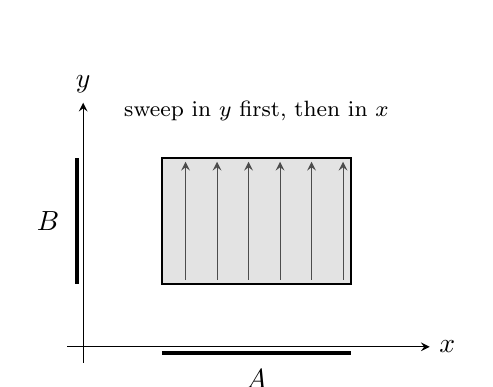
\begin{tikzpicture}[scale=1.0,>=stealth]
    \fill[gray!22] (1.0,0.8) rectangle (3.4,2.4);
    \draw[thick] (1.0,0.8) rectangle (3.4,2.4);
    \draw[->] (-0.2,0) -- (4.4,0) node[right] {$x$};
    \draw[->] (0,-0.2) -- (0,3.1) node[above] {$y$};
    \draw[very thick] (1.0,-0.08) -- (3.4,-0.08);
    \node[below] at (2.2,-0.16) {$A$};
    \draw[very thick] (-0.08,0.8) -- (-0.08,2.4);
    \node[left] at (-0.18,1.6) {$B$};
    \foreach \t in {1.3,1.7,2.1,2.5,2.9,3.3}
      \draw[->,gray!60!black] (\t,0.85) -- (\t,2.35);
    \node[align=center] at (2.2,3.0)
      {\footnotesize sweep in $y$ first, then in $x$};
  \end{tikzpicture}
  \hfill
  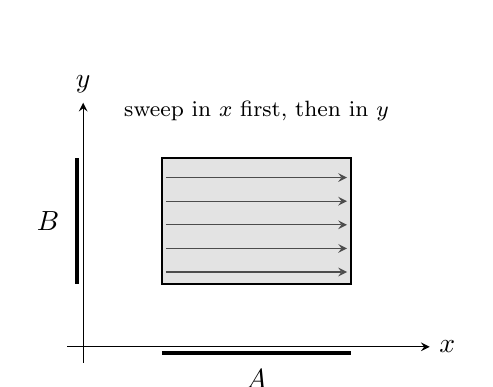
\begin{tikzpicture}[scale=1.0,>=stealth]
    \fill[gray!22] (1.0,0.8) rectangle (3.4,2.4);
    \draw[thick] (1.0,0.8) rectangle (3.4,2.4);
    \draw[->] (-0.2,0) -- (4.4,0) node[right] {$x$};
    \draw[->] (0,-0.2) -- (0,3.1) node[above] {$y$};
    \draw[very thick] (1.0,-0.08) -- (3.4,-0.08);
    \node[below] at (2.2,-0.16) {$A$};
    \draw[very thick] (-0.08,0.8) -- (-0.08,2.4);
    \node[left] at (-0.18,1.6) {$B$};
    \foreach \t in {0.95,1.25,1.55,1.85,2.15}
      \draw[->,gray!60!black] (1.05,\t) -- (3.35,\t);
    \node[align=center] at (2.2,3.0)
      {\footnotesize sweep in $x$ first, then in $y$};
  \end{tikzpicture}
  \vspace{0.3cm}
\end{figure}

\medskip
On the rectangle $A \times B$ both sweeps give $\mu(A) \nu(B)$, which is the
definition of the mesure produit; the théorème de Fubini says that the agreement
survives for every mesurable $f$, under one of its two hypotheses. The two branches
deserve separate names, because they are used differently.

\begin{remark}[Fubini--Tonelli and Fubini]
  For a \emph{positive} mesurable $f$ nothing further is required: the three
  integrals are equal in $[0,+\infty]$, all three being possibly infinite together.
  This branch is usually called \textbf{Fubini--Tonelli}, and it is the one that
  needs no verification beyond positivity. For a function of arbitrary sign,
  integrability with respect to $\mu \otimes \nu$ is required, and that is a genuine
  hypothesis to check. The standard procedure is therefore to use Tonelli on $|f|$ to
  establish integrability, and only then Fubini on $f$ --- two passes, never one. In
  both branches $\mu$ and $\nu$ must be $\sigma$-finies, without which $\mu \otimes
  \nu$ is not even defined.
\end{remark}

\begin{remark}[Testing integrability]
  Si la fonction $f$ n'est pas positive, on peut tester si elle est intégrable en
  appliquant le théorème de Fubini à la fonction $|f|$, which is positive, soit :
  \[
    \int |f(x,y)| \, d(\mu \otimes \nu)(x,y)
    = \int \left( \int |f(x,y)| \, d\nu(y) \right) d\mu(x)
    = \int \left( \int |f(x,y)| \, d\mu(x) \right) d\nu(y) .
  \]
  Either iterated integral of $|f|$ may be computed, whichever is easier, and
  finiteness of one of them is finiteness of all three.
\end{remark}

\begin{remark}[The inner integrals need not always exist]
  On prendra garde au fait, apparent dans la preuve du théorème, que les intégrales
  \[
    x \mapsto \int f(x,y) \, d\nu(y)
    \qquad \text{and} \qquad
    y \mapsto \int f(x,y) \, d\mu(x)
  \]
  ne sont pas toujours définies. Le fait qu'elles le soient \emph{presque partout}
  justifie l'écriture du théorème, and it is a conclusion of the theorem rather than
  a hypothesis.
\end{remark}

\begin{example}[Without integrability the two orders disagree]
  Let
  \[
    f(x,y) = \frac{x^{2} - y^{2}}{(x^{2} + y^{2})^{2}}
    \qquad \text{on } \, ]0,1[^{2} .
  \]
  Since $\frac{\partial}{\partial y} \left( \frac{y}{x^{2}+y^{2}} \right) = f(x,y)$,
  \[
    \int_{0}^{1} f(x,y) \, dy = \left[ \frac{y}{x^{2}+y^{2}} \right]_{0}^{1}
    = \frac{1}{1+x^{2}} ,
    \qquad \text{so} \qquad
    \int_{0}^{1} \left( \int_{0}^{1} f(x,y) \, dy \right) dx = \frac{\pi}{4} .
  \]
  But $f(y,x) = -f(x,y)$, so exchanging the roles of the variables gives
  \[
    \int_{0}^{1} \left( \int_{0}^{1} f(x,y) \, dx \right) dy = -\frac{\pi}{4} .
  \]
  The two iterated integrals differ. Both mesures are $\sigma$-finies, and $f$ is
  mesurable; the condition that fails is integrability. Indeed, on the triangle $0 <
  y < x < 1$ one has $x^{2} + y^{2} < 2x^{2}$ and therefore $f \geq
  \frac{x^{2}-y^{2}}{4x^{4}} \geq 0$, whose integral over that triangle is
  \[
    \int_{0}^{1} \frac{1}{4x^{4}} \left( x^{3} - \frac{x^{3}}{3} \right) dx
    = \frac{1}{6} \int_{0}^{1} \frac{dx}{x} = +\infty ,
  \]
  so $\int |f| \, dx \, dy = +\infty$. The example is the reason
  the two-pass procedure above is not a formality: a single careless application of
  Fubini here returns two different numbers for the same quantity.
\end{example}

Le théorème de Fubini justifie la notation plus simple
\[
  \int f(x,y) \, d\mu(x) \, d\nu(y)
  \qquad \text{or} \qquad
  \int f \, d\mu \, d\nu
\]
pour toute fonction mesurable $f$ positive ou intégrable. Ces résultats se
généralisent à toute fonction de $n$ variables. Pour toutes mesures $\sigma$-finies
$\mu_{1},\ldots,\mu_{n}$ sur les espaces mesurables respectifs
$(E_{1},\mathcal{E}_{1}),\ldots,(E_{n},\mathcal{E}_{n})$, on écrira
\[
  \int f(x_{1},\ldots,x_{n}) \, d\mu_{1}(x_{1}) \ldots d\mu_{n}(x_{n})
  \qquad \text{or} \qquad
  \int f \, d\mu_{1} \ldots d\mu_{n}
\]
pour toute fonction mesurable $f : E_{1} \times \ldots \times E_{n} \to
\bar{\reals}$ positive ou intégrable.

\subsection{Intégrale dépendant d'un paramètre}

Pour finir, on considère le cas d'une fonction $f$ de $x \in \Omega$ dépendant d'un
paramètre $t$. Son intégrale par rapport à une mesure $\mu$ sur $(\Omega,\mathcal{F})$
est une fonction de $t$. On s'intéresse à la continuité et à la dérivabilité de cette
fonction. Both answers are convergence dominée in disguise, and both carry a
domination hypothesis that is uniform in the parameter.

\begin{theorem}[Continuité sous le signe somme (\textit{continuity under the integral sign})]
  Soit $U$ un ouvert de $\reals^{n}$ et $f : \Omega \times U \to \bar{\reals}$ une
  fonction telle que :
  \begin{itemize}
    \item pour tout $t \in U$, la fonction $x \mapsto f(x,t)$ est mesurable ;
    \item pour presque tout $x \in \Omega$, la fonction $t \mapsto f(x,t)$ est
      continue ;
    \item il existe une fonction intégrable $g$ telle que $|f(x,t)| \leq g(x)$ pour
      presque tout $x \in \Omega$ et pour tout $t \in U$.
  \end{itemize}
  Alors la fonction $t \mapsto \int f(x,t) \, d\mu(x)$ est bien définie pour tout $t
  \in U$ et continue.
\end{theorem}

\begin{proof}
  Soit $t \in U$. Comme la fonction $x \mapsto f(x,t)$ est mesurable et que
  \[
    \int |f(x,t)| \, d\mu(x) \leq \int g(x) \, d\mu(x) < \infty ,
  \]
  son intégrale par rapport à la mesure $\mu$ est bien définie. Pour toute suite
  $(t_{n})_{n \geq 1}$ de $U$ tendant vers $t$, la suite de fonctions $(x \mapsto
  f(x,t_{n}))_{n \geq 1}$ tend p.p. vers la fonction $x \mapsto f(x,t)$ by the
  continuity hypothesis, and it is dominated by $g$. Par convergence dominée, on a :
  \[
    \lim_{n \to \infty} \int f(x,t_{n}) \, d\mu(x) = \int f(x,t) \, d\mu(x) ,
  \]
  so la fonction $t \mapsto \int f(x,t) \, d\mu(x)$ est continue en $t$.
\end{proof}

\begin{example}[Continuity of a parametrised Gaussian-type integral]
  Pour tout $t > 0$, la fonction
  \[
    t \mapsto \int e^{-tx^{4}} \, dx
  \]
  est continue. Il suffit d'appliquer le théorème sur tout ouvert $U =
  ]\epsilon,+\infty[$ avec $\epsilon > 0$, where $e^{-tx^{4}} \leq e^{-\epsilon
  x^{4}}$, an integrable dominating function independent of $t$.
\end{example}

\begin{remark}[The domination must not depend on the parameter]
  The point of the example is the restriction to $]\epsilon,+\infty[$. On the full
  half-line $]0,+\infty[$ there is no integrable $g$ dominating $e^{-tx^{4}}$ for
  every $t$ at once, since the integrand tends to the constant $1$ as $t \to 0$.
  Continuity is a local property, so proving it on every $]\epsilon,+\infty[$ proves
  it on $]0,+\infty[$; choosing the open set is part of applying the theorem, not a
  detail.
\end{remark}

\begin{theorem}[Dérivabilité sous le signe somme (\textit{differentiability under the integral sign})]
  Soit $U$ un ouvert de $\reals^{n}$ et $f : \Omega \times U \to \bar{\reals}$ une
  fonction telle que :
  \begin{itemize}
    \item pour tout $t \in U$, la fonction $x \mapsto f(x,t)$ est intégrable ;
    \item pour presque tout $x \in \Omega$, la fonction $t \mapsto f(x,t)$ est
      dérivable ;
    \item il existe une fonction intégrable $g$ telle que $\left| \frac{\partial
      f}{\partial t}(x,t) \right| \leq g(x)$ pour presque tout $x \in \Omega$ et pour
      tout $t \in U$.
  \end{itemize}
  Alors la fonction $t \mapsto \int f(x,t) \, d\mu(x)$ est bien définie pour tout $t
  \in U$, dérivable, et
  \[
    \frac{\partial}{\partial t} \int f(x,t) \, d\mu(x)
    = \int \frac{\partial f}{\partial t}(x,t) \, d\mu(x) .
  \]
\end{theorem}

\begin{proof}
  Soit $t \in U$. Pour toute suite $(t_{n})_{n \geq 1}$ de $U \setminus \{t\}$
  tendant vers $t$, la suite de fonctions
  \[
    \left( x \mapsto \frac{f(x,t_{n}) - f(x,t)}{t_{n} - t} \right)_{n \geq 1}
  \]
  tend p.p. vers la fonction $x \mapsto \frac{\partial f}{\partial t}(x,t)$, and by
  the mean value theorem each term is bounded in modulus by $g$. Par convergence
  dominée, on obtient :
  \[
    \lim_{n \to \infty} \frac{\int f(x,t_{n}) \, d\mu(x)
      - \int f(x,t) \, d\mu(x)}{t_{n} - t}
    = \lim_{n \to \infty} \int \frac{f(x,t_{n}) - f(x,t)}{t_{n} - t} \, d\mu(x)
    = \int \frac{\partial f}{\partial t}(x,t) \, d\mu(x) .
  \]
  La fonction $t \mapsto \int f(x,t) \, d\mu(x)$ est donc dérivable en $t$, de
  dérivée $\int \frac{\partial f}{\partial t}(x,t) \, d\mu(x)$.
\end{proof}

\begin{remark}[The domination is on the derivative, not on the function]
  The third hypothesis bounds $\frac{\partial f}{\partial t}$, not $f$ --- $f$ itself
  is handled by the first hypothesis, which asks only that each $x \mapsto f(x,t)$ be
  integrable. Confusing the two is the standard error. The domination is what turns
  the difference quotients, which converge pointwise but need not be uniformly small,
  into a sequence to which convergence dominée applies; the mean value theorem is
  what transfers a bound on the derivative to a bound on those quotients, and it is
  the reason the bound has to hold for every $t$ in $U$ and not merely at the point
  of interest.
\end{remark}

\begin{example}[Differentiating under the integral sign]
  Pour tout $t > 0$, la fonction
  \[
    t \mapsto \int e^{-tx^{2}} \, dx
  \]
  est dérivable, de dérivée :
  \[
    - \int x^{2} e^{-tx^{2}} \, dx .
  \]
  À nouveau, il suffit d'appliquer le théorème sur tout ouvert $U =
  ]\epsilon,+\infty[$ avec $\epsilon > 0$, where $\left| \frac{\partial}{\partial t} e^{-tx^{2}} \right| =
  x^{2} e^{-tx^{2}} \leq x^{2} e^{-\epsilon x^{2}}$, which is integrable and
  independent of $t$.
\end{example}

\begin{remark}[Where chapter 6 uses this]
  The fonction caractéristique of a variable aléatoire $X$ is $\varphi_{X}(t) =
  \expec(e^{itX})$, an integral depending on the parameter $t$. Continuité sous le
  signe somme gives its continuity with the constant $1$ as dominating function,
  available because a probability is a finite mesure; dérivabilité sous le signe
  somme gives, when $X$ is integrable, that $\varphi_{X}$ is differentiable with
  $\varphi_{X}'(t) = \expec(i X e^{itX})$, the dominating function being $|X|$.
  Iterating produces the moments of $X$ from the derivatives of $\varphi_{X}$ at the
  origin, which is what makes the fonction caractéristique useful at all.
\end{remark}

\begin{example}[A convergence computed by domination]
  Consider
  \[
    \lim_{n \to +\infty} \int_{0}^{+\infty}
      \left( 1 + \frac{x}{n} \right)^{n} e^{-2x} \, dx .
  \]
  The sequence $\left( 1 + \frac{x}{n} \right)^{n}$ increases to $e^{x}$ for every $x
  \geq 0$, so the integrands increase to $e^{-x}$; convergence monotone applies and
  gives
  \[
    \lim_{n \to +\infty} \int_{0}^{+\infty}
      \left( 1 + \frac{x}{n} \right)^{n} e^{-2x} \, dx
    = \int_{0}^{+\infty} e^{-x} \, dx = 1 .
  \]
  Convergence dominée gives the same answer, the whole sequence being bounded by the
  integrable $e^{-x}$; which of the two theorems one invokes is a matter of
  convenience, and here convergence monotone needs no dominating function at all.
\end{example}

\begin{conclusion}
  The chapter builds one object and proves six theorems about it. The object is the
  integral $\int f \, d\mu$, defined in three stages --- étagée positive, mesurable
  positive by a supremum, arbitrary sign by $f = f^{+} - f^{-}$ --- and every proof
  climbs those same three stages, which is why they are worth recognising as a single
  method rather than learning nine times.

  The six theorems are the working tools. Convergence monotone and convergence
  dominée exchange a limit and an integral, the first for an increasing sequence of
  positive functions with no further hypothesis, the second for any sequence
  dominated by a \emph{single integrable} function, with the lemme de Fatou between
  them giving an inequality that never fails. Transfer moves an integral from the
  abstract space to the value space, and is what makes a loi sufficient. The
  changement de variable carries the Jacobian in absolute value and requires a
  diffeomorphism, a $C^{1}$ bijection with non-vanishing Jacobian. Fubini exchanges
  the order of two integrations, needing $\sigma$-finiteness of both mesures and
  either positivity or integrability of the function --- which is why one tests
  integrability with Tonelli on $|f|$ before applying Fubini to $f$. Continuité sous
  le signe somme and dérivabilité sous le signe somme are convergence dominée applied
  to a parametrised family, the domination being on $f$ in the first case and on
  $\frac{\partial f}{\partial t}$ in the second.

  The hypotheses that go missing under compression are all of one kind, a finiteness
  or positivity condition attached to an interchange: the integrability of the
  dominating function, the $\sigma$-finiteness in Fubini and in Radon--Nikodym, the
  absolute integrability an intégrale de Riemann impropre need not have, and the
  finiteness that lets one of $f$, $g$ be subtracted in the additivity of the
  integral. Each has a one-line counter-example above. The next chapter re-reads all
  of this with $\mu$ a mesure de probabilité: the integral becomes the espérance,
  transfer becomes the passage from a variable aléatoire to its loi, and the
  convergence theorems become the tools of the limit theorems at the end of the
  course.
\end{conclusion}

\section{Théorie des probabilités}

Modern probability is the théorie de la mesure with one extra axiom: the total mass
is one. Everything in this chapter is a specialisation of chapters 2 and 3 --- a
probability is a mesure, a variable aléatoire is a mesurable function, an espérance
is an intégrale de Lebesgue --- and the work is in learning what the specialisation
buys. What it buys is a vocabulary that the general theory does not have: lois,
fonctions de répartition, densités, indépendance, moments, and the three
inequalities that every limit theorem in chapter 8 rests on.\\

Les résultats présentés généralisent ceux vus au chapitre 1 dans le cas des
probabilités discrètes. Certaines preuves, identiques dans les deux cas, sont
omises: those that are the discrete one word for word, with a sum replaced by an
integral. Where the technique is one an exam asks for, it is carried in full. Two
such techniques dominate the chapter. The first is the fonction test method of computing a densité, which is the single
most-used calculation in the written papers. The second is the supporting-line
argument behind the inégalité de Jensen,
which reappears whenever convexity is used.

\subsection{Espace de probabilité}

Soit $(\Omega,\mathcal{F})$ un espace mesurable.

\begin{definition}[Mesure de probabilité]
  On appelle \textbf{mesure de probabilité} sur $(\Omega,\mathcal{F})$ toute
  mesure, notée $\prob$, telle que $\prob(\Omega)=1$.
\end{definition}

On note qu'on ne pourra définir la probabilité que de certains sous-ensembles de
$\Omega$ : les éléments de la tribu $\mathcal{F}$, which get their own name.

\begin{definition}[Événement]
  On appelle \textbf{événement} tout élément de la tribu $\mathcal{F}$.
\end{definition}

Un événement de probabilité $1$ est dit presque sûr (p.s.\ en abrégé). The
triple $(\Omega,\mathcal{F},\prob)$ is an \textbf{espace de probabilité}
(\textit{probability space}).

\begin{example}[Mesure de Lebesgue restreinte à l'intervalle unité]
  La mesure de Lebesgue $\lambda$ sur l'ensemble $\Omega = [0,1]$ muni de la
  tribu de Borel est une mesure de probabilité, since $\lambda([0,1])=1$. This is
  the canonical source of a uniform variable aléatoire.
\end{example}

\begin{example}[A finite discrete probability]
  La mesure discrète
  \[
    \prob = \tfrac{1}{3}\left(\delta_{1}+\delta_{2}+\delta_{3}\right)
  \]
  sur l'ensemble $\Omega = \{1,2,3\}$ muni de sa tribu des parties
  $\mathcal{P}(\Omega)$ est une mesure de probabilité. It puts mass $\tfrac13$ on
  each atom.
\end{example}

On a les propriétés élémentaires suivantes, comme dans le cas discret; they
follow from $\sigma$-additivité and from the general properties of a mesure.

\begin{prop}
  Pour tous événements $A,B$ :
  \begin{enumerate}
    \item $\prob(A^{c}) = 1 - \prob(A)$;
    \item $\prob(A \union B) = \prob(A) + \prob(B) - \prob(A \intersect B)$;
    \item si $A \subr B$, alors $\prob(A) \leq \prob(B)$.
  \end{enumerate}
\end{prop}

\begin{remark}
  La première propriété est une conséquence de la $\sigma$-additivité, applied to
  the partition $\Omega = A \dunion A^{c}$, which gives
  $\prob(A)+\prob(A^{c}) = \prob(\Omega) = 1$; this is the only place the total
  mass being $1$ is used. Les 2 dernières propriétés sont une transcription au cas
  d'une mesure de probabilité of chapter 2's inclusion--exclusion and monotonicity
  for a general mesure.
\end{remark}

On a également les propriétés de convergence monotone et la borne de l'union,
comme dans le cas discret.

\begin{prop}
  Soit $(A_{n})_{n \geq 1}$ une suite d'événements.
  \begin{enumerate}
    \item Si $A_{n} \uparrow A$, alors $\prob(A) = \lim_{n} \uparrow \prob(A_{n})$.
    \item Si $A_{n} \downarrow A$, alors $\prob(A) = \lim_{n} \downarrow \prob(A_{n})$.
    \item On a la borne de l'union :
      \[
        \prob\Big(\bigcup_{n \geq 1} A_{n}\Big) \leq \sum_{n \geq 1} \prob(A_{n}).
      \]
  \end{enumerate}
\end{prop}

\begin{remark}
  The decreasing case is the one that needs the finite total mass. For a general
  mesure $\mu$, $A_{n} \downarrow A$ gives $\mu(A) = \lim_{n} \mu(A_{n})$ only
  when some $A_{n_{0}}$ has finite mesure; under a mesure de probabilité every
  événement has mesure at most $1$, so the condition is automatic and the
  hypothesis disappears. The borne de l'union needs no hypothesis at all.
\end{remark}

Les résultats sur l'indépendance et le conditionnement sont identiques au cas
discret, with the same proofs: $A \indep B$ means
$\prob(A \intersect B) = \prob(A)\prob(B)$, and
$\prob(A \mid B) = \prob(A \intersect B)/\prob(B)$ whenever $\prob(B) > 0$. The
formule de Bayes and the formule des probabilités totales carry over unchanged.
What does not carry over is conditioning on an événement of probability zero,
which is chapter 5's subject.

\subsection{Variables aléatoires}

Soit $(E,\mathcal{E})$ un espace mesurable --- a second one, the space of values.

\begin{definition}[Variable aléatoire]
  Une \textbf{variable aléatoire} $X$ à valeurs dans $E$ est une fonction
  mesurable de $(\Omega,\mathcal{F})$ vers $(E,\mathcal{E})$.
\end{definition}

Measurability is the whole of the definition: $X$ is a variable aléatoire precisely
when $X^{-1}(A) \in \mathcal{F}$ for every $A \in \mathcal{E}$, so that
$\prob(X \in A)$ makes sense for every $A$. Toute variable aléatoire définit une
mesure de probabilité, appelée la loi: it pushes the mesure de probabilité forward
onto its value space.

\begin{definition}[Loi d'une variable aléatoire]
  On appelle \textbf{loi} de la variable aléatoire $X$, notée $\prob_{X}$, la
  mesure image de $\prob$ par $X$ :
  \[
    \forall A \in \mathcal{E}, \qquad \prob_{X}(A) = \prob(X \in A).
  \]
\end{definition}

The loi is a mesure de probabilité on $(E,\mathcal{E})$: it is a mesure because
preimages preserve disjoint countable unions, and its total mass is
$\prob(X \in E) = \prob(\Omega) = 1$.

\begin{example}[A Bernoulli variable built on the unit interval]
  Soit $\Omega = [0,1]$ muni de la tribu de Borel, et $\prob$ la mesure de
  Lebesgue. The variable aléatoire $X = \indic_{[0,1/2]}$ takes the values $0$ and
  $1$, and
  \[
    \prob(X=1) = \prob\!\left(\left[0,\tfrac12\right]\right) = \tfrac12 ,
  \]
  so $X$ follows the loi de Bernoulli $\mathcal{B}(\tfrac12)$. The same
  construction with $[0,p]$ produces $\mathcal{B}(p)$ for any $p \in [0,1]$.
\end{example}

\begin{remark}[The espace de probabilité is almost never named]
  En pratique, l'espace de probabilité $(\Omega,\mathcal{F},\prob)$ est rarement
  spécifié. Il s'agit d'un espace abstrait, suffisamment riche pour modéliser le
  problème d'intérêt, mais la plupart du temps sans lien avec la ``physique'' de
  l'expérience aléatoire considérée. La \emph{loi} $\prob_{X}$ de la variable
  aléatoire suffit pour les calculs, sans besoin de connaître l'espace de
  probabilité sous-jacent: every computation in this chapter and the next four is
  done from it, never from $\Omega$. The example above is worth remembering only
  because it shows that a rich enough space exists: the unit interval under the
  mesure de Lebesgue already carries a variable of any prescribed loi, namely
  $F^{-1}(U)$ for $U$ the identity map on $[0,1]$ and $F$ the desired fonction de
  répartition. Here $F^{-1}$ has to be read as the generalised inverse
  $F^{-1}(u) = \inf\{x \in \reals : F(x) \geq u\}$: the ordinary inverse exists
  only for $F$ continuous and strictly increasing, and would already fail for the
  loi de Bernoulli just built.
\end{remark}

\begin{prop}
  Deux variables aléatoires $X$, $Y$ telles que $X = Y$ p.s.\ ont même loi.
\end{prop}

\begin{remark}
  Soit $B$ l'événement $\{X = Y\}$, qui appartient bien à la tribu $\mathcal{F}$
  car $X - Y$ est une variable aléatoire. Comme $\prob(B)=1$, intersecting with
  $B$ changes no probability, and for every $A \in \mathcal{E}$,
  $\prob_{X}(A) = \prob(X^{-1}(A) \intersect B)
   = \prob(Y^{-1}(A) \intersect B) = \prob_{Y}(A)$.
  The converse is false, and badly so: two variables can have the same loi while
  being presque sûrement different, as $X$ and $1-X$ are for $X$ uniform on
  $[0,1]$.
\end{remark}

\subsection{Fonction de répartition}

Lorsque $E = \reals$ muni de la tribu de Borel $\mathcal{B}(\reals)$, la loi de
$X$ peut être décrite par sa fonction de répartition, a single function of a real
variable.

\begin{definition}[Fonction de répartition]
  La \textbf{fonction de répartition} (\textit{cumulative distribution function})
  d'une variable aléatoire réelle $X$ est la fonction $F_{X}$ définie par :
  \[
    \forall x \in \reals, \qquad F_{X}(x) = \prob(X \leq x).
  \]
\end{definition}

La fonction de répartition permet de caractériser la loi car
$F_{X}(x) = \prob_{X}(\left]-\infty,x\right])$. La collection des intervalles
$\left]-\infty,x\right]$ avec $x \in \reals$ étant stable par intersection finie
et engendrant la tribu de Borel $\mathcal{B}(\reals)$, c'est en effet une
conséquence du théorème d'unicité. That theorem of chapter 2 says that two
mesures de probabilité agreeing on such a family agree on the whole tribu de
Borel. This is the fact chapter 8's definition of the convergence en loi is built
on, so it is worth stating as a property in its own right rather than as a
passing observation.

\begin{prop}
  La fonction de répartition $F_{X}$ est une fonction croissante, continue à
  droite, telle que :
  \[
    \lim_{x \to -\infty} F_{X}(x) = 0
    \qquad\text{and}\qquad
    \lim_{x \to +\infty} F_{X}(x) = 1 .
  \]
  Moreover $F_{X}$ determines $\prob_{X}$ completely: two variables aléatoires
  réelles with the same fonction de répartition have the same loi.
\end{prop}

\begin{remark}
  All four properties are convergence monotone for the mesure $\prob_{X}$, read
  on nested intervals. Monotonicity is
  $\left]-\infty,x\right] \subr \left]-\infty,y\right]$ for $x \leq y$.
  Right-continuity is
  $\left]-\infty,x+\tfrac1n\right] \downarrow \left]-\infty,x\right]$, which needs
  the decreasing case of the previous section and therefore the finite total mass.
  The two limits are
  $\left]-\infty,x\right] \downarrow \emptyset$ and
  $\left]-\infty,x\right] \uparrow \reals$. The last sentence is the théorème
  d'unicité, as above.
\end{remark}

La fonction de répartition n'est pas toujours continue. Ses éventuels points de
discontinuités correspondent aux ``atomes'' de la loi, c'est-à-dire aux singletons
de mesure non nulle, and the size of the jump is the mass of the atom:
\[
  \forall x \in \reals, \qquad
  \prob(X = x) = \prob(X \leq x) - \prob(X < x) = F_{X}(x) - F_{X}(x^{-}),
\]
où $F_{X}(x^{-})$ désigne la limite à gauche de $F_{X}$ en $x$. Being
non-decreasing, $F_{X}$ has a left limit everywhere, so this is well defined at
every point.

\begin{definition}[Loi diffuse]
  Une loi sans atome, c'est-à-dire dont la fonction de répartition est continue,
  est dite \textbf{diffuse}.
\end{definition}

\begin{example}[The loi uniforme, a continuous staircase-free fonction de répartition]
  Une variable aléatoire $X$ suivant une loi uniforme sur $[0,1]$ a pour fonction
  de répartition :
  \[
    F_{X}(x) =
    \begin{cases}
      0 & \text{if } x < 0,\\
      x & \text{if } x \in [0,1],\\
      1 & \text{if } x \geq 1.
    \end{cases}
  \]
  Cette fonction est continue, so the loi is diffuse and $\prob(X=x)=0$ for every
  $x$.
\end{example}

\begin{example}[The loi de Bernoulli, a fonction de répartition with two jumps]
  Une variable aléatoire $X \sim \mathcal{B}(p)$, de paramètre $p \in [0,1]$, a
  pour fonction de répartition :
  \[
    F_{X}(x) =
    \begin{cases}
      0 & \text{if } x < 0,\\
      1-p & \text{if } x \in [0,1[,\\
      1 & \text{if } x \geq 1 .
    \end{cases}
  \]

  \begin{remark}
    The middle value is $1-p$: on $[0,1[$, that is for
    $0 \leq x < 1$, $F(x) = \prob(X \leq x)$ is $\prob(X = 0) = 1-p$. The figure
    below, drawn for $p$ equal to $1/3$, puts the step at height $1-p$.
  \end{remark}
  Cette fonction est discontinue: it jumps by $1-p$ at $0$ and by $p$ at $1$,
  which are exactly $\prob(X=0)$ and $\prob(X=1)$.
\end{example}

\begin{figure}[htbp]
  \centering
  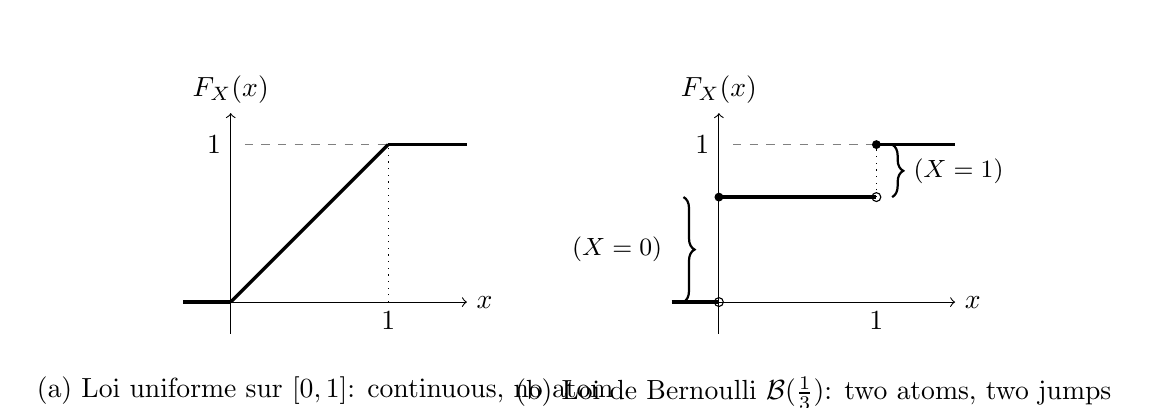
\begin{tikzpicture}[scale=1.0]
    % --- left panel: continuous CDF (uniform on [0,1])
    \begin{scope}
      \draw[->] (-0.6,0) -- (3.0,0) node[right] {$x$};
      \draw[->] (0,-0.4) -- (0,2.4) node[above] {$F_{X}(x)$};
      \draw[dashed,gray] (0.18,2) -- (3.0,2);
      \node[left] at (0,2) {$1$};
      \draw[very thick] (-0.6,0) -- (0,0);
      \draw[very thick] (0,0) -- (2,2);
      \draw[very thick] (2,2) -- (3.0,2);
      \node[below] at (2,0) {$1$};
      \draw[dotted] (2,0) -- (2,2);
      \node[below=12pt] at (1.2,-0.4) {(a) Loi uniforme sur $[0,1]$: continuous, no atom};
    \end{scope}
    % --- right panel: discrete CDF (Bernoulli 1/3)
    \begin{scope}[xshift=6.2cm]
      \draw[->] (-0.6,0) -- (3.0,0) node[right] {$x$};
      \draw[->] (0,-0.4) -- (0,2.4) node[above] {$F_{X}(x)$};
      \draw[dashed,gray] (0.18,2) -- (3.0,2);
      \node[left] at (0,2) {$1$};
      \draw[very thick] (-0.6,0) -- (0,0);
      \draw[very thick] (0,1.3333) -- (2,1.3333);
      \draw[very thick] (2,2) -- (3.0,2);
      \fill (0,1.3333) circle (1.6pt);
      \draw (0,0) circle (1.6pt);
      \fill (2,2) circle (1.6pt);
      \draw (2,1.3333) circle (1.6pt);
      \draw[dotted] (0,0) -- (0,1.3333);
      \draw[dotted] (2,1.3333) -- (2,2);
      \node[below] at (2,0) {$1$};
      \draw[decorate,decoration={brace,amplitude=4pt},thick]
        (-0.45,1.3333) -- (-0.45,0)
        node[midway,left=4pt] {\small $\prob(X=0)$};
      \draw[decorate,decoration={brace,amplitude=4pt,mirror},thick]
        (2.2,1.3333) -- (2.2,2)
        node[midway,right=4pt] {\small $\prob(X=1)$};
      \node[below=12pt] at (1.2,-0.4) {(b) Loi de Bernoulli $\mathcal{B}(\tfrac13)$: two atoms, two jumps};
    \end{scope}
  \end{tikzpicture}
  \caption{A continuous fonction de répartition beside a staircase one. Every jump
  of a fonction de répartition is an atom of the loi, and its height is that atom's
  probability.}
\end{figure}

\begin{example}[A loi has at most countably many atoms]
  For each $n \geq 1$, the set of atoms of mass at least $1/n$ has at most $n$
  elements, since the masses of distinct atoms are the mesures of disjoint sets
  and sum to at most $1$. The set of all atoms is the union over $n$ of these
  finite sets, hence at most countable. So a fonction de répartition, however
  wild, has at most countably many discontinuities --- and a loi whose support is
  uncountable must give mass zero to all but countably many of its points.
\end{example}

\subsection{Lois à densité}

On dit qu'une variable aléatoire réelle a une densité lorsque sa loi a une densité
par rapport à la mesure de Lebesgue, in the sense of chapter 3.

\begin{definition}[Variable à densité]
  Une variable aléatoire réelle $X$ a pour \textbf{densité} la fonction $f_{X}$ si :
  \[
    \forall A \in \mathcal{B}(\reals), \qquad
    \prob_{X}(A) = \int_{A} f_{X}(x)\,dx .
  \]
\end{definition}

La fonction de densité $f_{X}$ est mesurable, positive, et telle que :
\[
  \int_{-\infty}^{+\infty} f_{X}(x)\,dx = 1 ,
\]
which is the statement $\prob_{X}(\reals)=1$. Conversely any mesurable
non-negative function integrating to $1$ is the densité of some loi. Une loi à
densité est diffuse puisque :
\[
  \forall x \in \reals, \qquad \prob(X=x) = \prob_{X}(\{x\}) = \int_{\{x\}} f_{X} = 0
\]
--- a singleton is négligeable for the mesure de Lebesgue. La fonction de
répartition est donnée par :
\[
  \forall x \in \reals, \qquad F_{X}(x) = \prob(X \leq x) = \int_{-\infty}^{x} f_{X}(u)\,du ,
\]
une fonction continue, presque partout dérivable, de dérivée $f_{X}$ en chaque
point de dérivabilité.

\begin{example}[The three densités used constantly]
  Loi uniforme sur $[0,1]$ : $f_{X} = \indic_{[0,1]}$. \\
  Loi exponentielle $\mathcal{E}(\lambda)$ de paramètre $\lambda > 0$ :
  $f_{X}(x) = \lambda e^{-\lambda x} \indic_{\reals_{+}}(x)$. \\
  \textbf{Loi normale} (\textit{normal distribution}) centrée réduite
  $\mathcal{N}(0,1)$ :
  $f_{X}(x) = \frac{1}{\sqrt{2\pi}} e^{-x^{2}/2}$.
\end{example}

\begin{figure}[htbp]
  \centering
  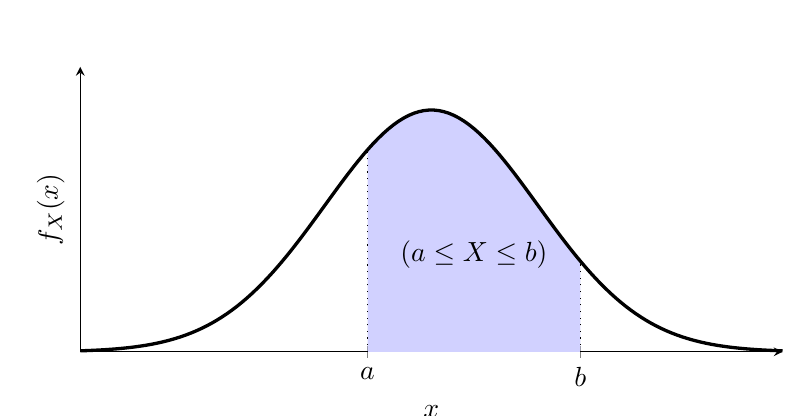
\begin{tikzpicture}
    \begin{axis}[
      width=10.5cm, height=5.2cm,
      axis lines=left,
      xlabel={$x$}, ylabel={$f_{X}(x)$},
      xmin=-3.3, xmax=3.3, ymin=0, ymax=0.47,
      xtick={-0.6,1.4}, xticklabels={$a$,$b$},
      ytick=\empty,
      clip=false,
      ]
      \addplot[name path=fab, domain=-0.6:1.4, samples=80, draw=none]
        {exp(-x^2/2)/sqrt(2*pi)};
      \addplot[name path=axab, domain=-0.6:1.4, samples=2, draw=none] {0};
      \addplot[fill=blue!18] fill between[of=fab and axab];
      \addplot[very thick, black, domain=-3.3:3.3, samples=140]
        {exp(-x^2/2)/sqrt(2*pi)};
      \draw[dotted] (axis cs:-0.6,0) -- (axis cs:-0.6,0.3332);
      \draw[dotted] (axis cs:1.4,0) -- (axis cs:1.4,0.1497);
      \node at (axis cs:0.4,0.16) {$\prob(a \leq X \leq b)$};
    \end{axis}
  \end{tikzpicture}
  \caption{For a loi à densité, a probability is an area. The shaded region
  is $\int_{a}^{b} f_{X}(x)\,dx = F_{X}(b)-F_{X}(a) = \prob(a \leq X \leq b)$,
  and the endpoints may be included or excluded freely because the loi is
  diffuse.}
\end{figure}

\paragraph{Existence d'une densité.}
Une question intéressante est la réciproque : une loi dont la fonction de
répartition $F_{X}$ est continue et presque partout dérivable admet-elle une
densité ? La réponse est non, and the counter-example below is the standard one.
Il faut des conditions supplémentaires. Une condition suffisante est que la
fonction de répartition $F_{X}$ soit $C^{1}$, ou continue et $C^{1}$ par
morceaux. Par le théorème fondamental de l'analyse, on obtient alors :
\[
  \forall x \in \reals, \qquad F_{X}(x) = \int_{-\infty}^{x} F_{X}'(u)\,du ,
\]
où la dérivée $F_{X}'$ est définie à un ensemble négligeable près. La loi a donc
pour densité la fonction $f_{X} = F_{X}'$. This is worth writing down as a recipe:
\emph{if the fonction de répartition is continuous and piecewise $C^{1}$,
differentiate it, and the pieces where it is constant contribute zero.}

\begin{example}[Reading a densité off a piecewise-linear fonction de répartition]
  Soit
  \[
    F(x) =
    \begin{cases}
      0 & x \leq 0,\\
      \tfrac{x}{4} & x \in [0,1],\\
      \tfrac{3x-2}{4} & x \in [1,2],\\
      1 & x \geq 2 .
    \end{cases}
  \]
  This is non-decreasing (the slopes $\tfrac14$ and $\tfrac34$ are positive),
  continuous at $0$, $1$ and $2$, and has the right limits at $\pm\infty$, so it
  is the fonction de répartition of some variable aléatoire réelle $X$. La
  fonction est continue et $C^{1}$ par morceaux. La loi de $X$ a donc une densité,
  qui s'obtient en dérivant on each piece :
  \[
    f(x) = \tfrac14 \indic_{[0,1]}(x) + \tfrac34 \indic_{[1,2]}(x) .
  \]
  The two corner points $x=1$ and $x=2$ are négligeables and the value assigned
  to them is irrelevant.
\end{example}

\begin{example}[A truncated exponential has no densité]
  Soit $X = \min(Y,1)$, où $Y \sim \mathcal{E}(\lambda)$. For $x < 0$,
  $F_{X}(x) = 0$; for $x \in [0,1[$, $F_{X}(x) = 1-e^{-\lambda x}$; and
  $F_{X}(x)=1$ for $x \geq 1$. The function jumps at $x=1$ by
  $1 - (1-e^{-\lambda}) = e^{-\lambda} = \prob(Y \geq 1)$, so the loi has an atom
  at $1$ and cannot have a densité. Continuity of the fonction de répartition is a
  \emph{necessary} condition, and it is the first thing to check.
\end{example}

\begin{example}[The loi de Pareto, differentiated from its tail]
  Soit $X$ une variable aléatoire de loi de Pareto de paramètre $a > 0$, définie
  par $\prob(X > x) = x^{-a}$ pour $x \geq 1$. Then
  \[
    F_{X}(x) =
    \begin{cases}
      0 & \text{if } x \leq 1,\\
      1 - \dfrac{1}{x^{a}} & \text{otherwise},
    \end{cases}
    \qquad\text{hence}\qquad
    f_{X}(x) =
    \begin{cases}
      0 & \text{if } x \leq 1,\\
      \dfrac{a}{x^{a+1}} & \text{otherwise}.
    \end{cases}
  \]
  La fonction de répartition est une fonction $C^{1}$ par morceaux, and it is continuous at $x=1$, which is
  what licenses the differentiation.
\end{example}

\begin{example}[The devil's staircase: continuous, diffuse, and with no densité]
  Soit $X$ une variable aléatoire de loi uniforme sur l'ensemble de Cantor $C$.
  Comme cet ensemble $C$ est en bijection avec $[0,1]$, la loi de $X$ est diffuse.
  Sa fonction de répartition est continue et presque partout dérivable, de dérivée
  nulle presque partout, and it is non-decreasing --- it rises only on a set
  négligeable for the mesure de Lebesgue. Pourtant, la loi ne peut avoir de
  densité : $\prob_{X}(C) = 1$ alors que $\lambda(C) = 0$, so no integral of a
  function against the mesure de Lebesgue can reproduce $\prob_{X}$. This is why
  ``continue et presque partout dérivable'' is not enough.
\end{example}

\begin{remark}[Absolue continuité]
  Une condition nécessaire et suffisante d'existence d'une densité est l'absolue
  continuité de la fonction de répartition $F_{X}$ : pour tout $\varepsilon > 0$,
  il doit exister $\delta > 0$ tel que pour tout ensemble fini d'intervalles
  disjoints, l'écart cumulé de $F_{X}$ sur ces intervalles n'excède pas
  $\varepsilon$ si la longueur totale de ces intervalles n'excède pas $\delta$.
  C'est équivalent à dire que la loi de la variable aléatoire $X$ est absolument
  continue par rapport à la mesure de Lebesgue, and the densité is then the
  Radon--Nikodym derivative. The devil's staircase fails this: intervals of tiny
  total length covering $C$ carry the whole increase of $F_{X}$.
\end{remark}

\paragraph{Unicité de la densité.}
Une fonction de densité est unique à un ensemble négligeable près par rapport à
la mesure de Lebesgue, by chapter 3's uniqueness result for Radon--Nikodym
derivatives. Pour la loi uniforme sur $[0,1]$ par exemple, the values $f_{X}(0)$
and $f_{X}(1)$ are immaterial, and $\indic_{[0,1]}$, $\indic_{]0,1[}$ and
$\indic_{[0,1[}$ are the same densité. Every identity between densités below is
therefore an identity p.p., and that qualification is not decoration.

\subsection{Loi jointe, lois marginales}

Soit $X$ et $Y$ deux variables aléatoires à valeurs respectives dans les
ensembles $E$ et $E'$, munis des tribus respectives $\mathcal{E}$ et
$\mathcal{E}'$. Le couple $(X,Y)$ définit une variable aléatoire à valeurs dans
l'espace produit $E \times E'$ muni de la tribu $\mathcal{E} \otimes
\mathcal{E}'$, the tribu produit. Sa loi $\prob_{X,Y}$ est appelée la loi jointe;
les lois $\prob_{X}$, $\prob_{Y}$ en sont les lois marginales, recovered by
$\prob_{X}(A) = \prob_{X,Y}(A \times E')$.

\begin{definition}[Indépendance de deux variables aléatoires]
  Deux variables aléatoires $X$ et $Y$ sont dites \textbf{indépendantes} si pour
  tous $A \in \mathcal{E}$ et $B \in \mathcal{E}'$, les événements $\{X \in A\}$
  et $\{Y \in B\}$ sont indépendants, soit :
  \[
    \prob(X \in A,\, Y \in B) = \prob(X \in A)\,\prob(Y \in B).
  \]
\end{definition}

\begin{prop}[Indépendance et mesure]
  Deux variables aléatoires $X$ et $Y$ sont indépendantes si et seulement si leur
  loi jointe est la mesure produit :
  \[
    \prob_{X,Y} = \prob_{X} \otimes \prob_{Y} .
  \]
\end{prop}

\begin{remark}
  The definition says exactly that the two mesures agree on rectangles
  $A \times B$. Rectangles are stable par intersection finie and generate the
  tribu produit, so the proposition is une conséquence de l'unicité de la mesure
  produit (chapter 3), which upgrades agreement on rectangles to equality. The
  lois marginales never determine the loi jointe on their own; indépendance is
  precisely the extra information that they do.
\end{remark}

\paragraph{Fonction de répartition.}
Lorsque $E = E' = \reals$ muni de la tribu de Borel, le couple $(X,Y)$ est à
valeurs dans $\reals^{2}$. Comme pour les variables aléatoires réelles, sa loi
peut être décrite par sa fonction de répartition, the joint one, définie par :
\[
  \forall x,y \in \reals, \qquad F_{X,Y}(x,y) = \prob(X \leq x,\, Y \leq y).
\]

\begin{prop}[Indépendance et fonction de répartition]
  Deux variables aléatoires réelles $X$ et $Y$ sont indépendantes si et seulement
  si :
  \[
    \forall x,y \in \reals, \qquad F_{X,Y}(x,y) = F_{X}(x) F_{Y}(y).
  \]
\end{prop}

\begin{remark}
  One direction is the definition applied to
  $A = \left]-\infty,x\right]$, $B = \left]-\infty,y\right]$. The other is again
  uniqueness: the quadrants
  $\left]-\infty,x\right] \times \left]-\infty,y\right]$ form a family stable par
  intersection finie and generating $\mathcal{B}(\reals^{2})$, so equality of the
  two mesures there is equality everywhere.
\end{remark}

\paragraph{Lois à densité.}
Le couple $(X,Y)$ a une densité par rapport à la mesure de Lebesgue sur
$\reals^{2}$ s'il existe une fonction mesurable
$f_{X,Y} : \reals^{2} \to \reals_{+}$ telle que :
\[
  \forall A,B \in \mathcal{B}(\reals), \qquad
  \prob(X \in A,\, Y \in B) = \int_{A \times B} f_{X,Y}(x,y)\,dx\,dy ,
\]
sa fonction de répartition étant alors donnée par :
\[
  \forall x,y \in \reals, \qquad
  F_{X,Y}(x,y) = \int_{-\infty}^{x}\!\!\int_{-\infty}^{y} f_{X,Y}(u,v)\,du\,dv .
\]
Par le théorème de Fubini --- applicable because $f_{X,Y}$ is non-negative and
the mesure de Lebesgue on each factor is $\sigma$-finie --- les lois marginales
ont des densités, obtained by integrating out the other variable and données
respectivement par :
\[
  \forall x \in \reals,\ f_{X}(x) = \int_{\reals} f_{X,Y}(x,y)\,dy
  \qquad\text{and}\qquad
  \forall y \in \reals,\ f_{Y}(y) = \int_{\reals} f_{X,Y}(x,y)\,dx .
\]

\begin{prop}[Indépendance et densité]
  Deux variables aléatoires réelles $X$ et $Y$ dont la loi jointe a une densité
  $f_{X,Y}$ par rapport à la mesure de Lebesgue sont indépendantes si et seulement
  si :
  \[
    \forall x,y \in \reals, \qquad f_{X,Y}(x,y) = f_{X}(x) f_{Y}(y) \quad \text{p.p.}
  \]
\end{prop}

\begin{remark}
  Sufficiency is a double integration: if the densité factorises then
  $F_{X,Y}(x,y) = F_{X}(x)F_{Y}(y)$ and the previous proposition applies.
  Necessity runs the other way. Pour montrer que la condition est nécessaire, on écrit, by
  indépendance,
  $F_{X,Y}(x,y) = F_{X}(x)F_{Y}(y)
   = \int_{-\infty}^{x}\!\int_{-\infty}^{y} f_{X}(u)f_{Y}(v)\,du\,dv$,
  ce qui montre que la loi jointe a pour densité la fonction
  $(x,y) \mapsto f_{X}(x)f_{Y}(y)$ --- \emph{a} densité of it, not necessarily
  the given one. Le résultat est une conséquence de l'unicité de la densité à un
  ensemble négligeable près. That last step is why the conclusion is stated p.p.\
  and not pointwise.
\end{remark}

\begin{prop}[Existence d'une densité pour un couple]
  Si $X$ et $Y$ sont des variables aléatoires réelles indépendantes de densités
  respectives $f_{X}$ et $f_{Y}$, alors le couple $(X,Y)$ a pour densité :
  \[
    \forall x,y \in \reals, \qquad f_{X,Y}(x,y) = f_{X}(x) f_{Y}(y).
  \]
\end{prop}

\begin{remark}
  Comme précédemment, c'est une conséquence du théorème de Fubini: indépendance
  gives $F_{X,Y} = F_{X}F_{Y}$, each factor is an integral of its densité, and
  Fubini turns the product of two single integrals into one double integral. Note
  the direction: indépendance plus marginal densités gives a joint densité.
  Marginal densités alone do not --- see the pair $(X,X)$ below, whose lois
  marginales both have densités and which has none.
\end{remark}

\begin{figure}[htbp]
  \centering
  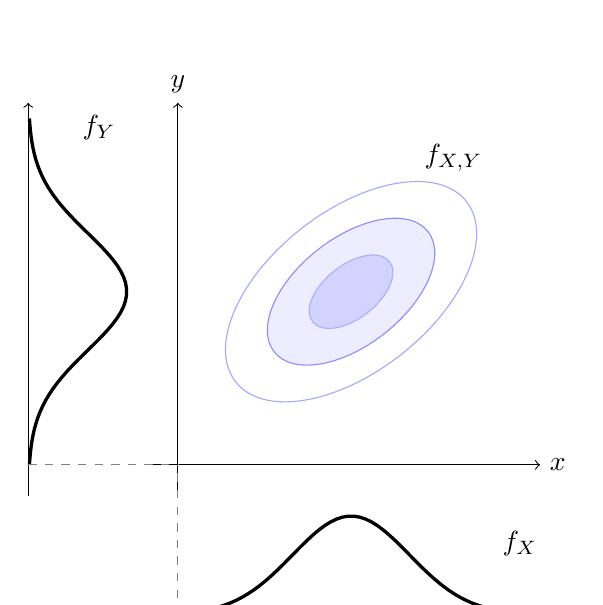
\begin{tikzpicture}[scale=1.0]
    % joint density: level sets of a correlated bivariate normal
    \begin{scope}[shift={(0,0)}]
      \draw[->] (-0.4,0) -- (4.6,0) node[right] {$x$};
      \draw[->] (0,-0.4) -- (0,4.6) node[above] {$y$};
      \begin{scope}[shift={(2.2,2.2)}, rotate=38]
        \draw[fill=blue!22, draw=blue!55] (0,0) ellipse (0.62 and 0.34);
        \draw[fill=blue!13, draw=blue!45, fill opacity=0.55] (0,0) ellipse (1.24 and 0.68);
        \draw[draw=blue!35] (0,0) ellipse (1.86 and 1.02);
      \end{scope}
      \node at (3.5,3.9) {$f_{X,Y}$};
    \end{scope}
    % marginal in x, drawn below the box
    \begin{scope}[shift={(0,-1.9)}]
      \draw[->] (-0.4,0) -- (4.6,0);
      \draw[very thick, black]
        plot[domain=0:4.4, samples=60] (\x, {1.25*exp(-(\x-2.2)*(\x-2.2)/1.1)});
      \node[right] at (4.0,0.9) {$f_{X}$};
    \end{scope}
    % marginal in y, drawn left of the box
    \begin{scope}[shift={(-1.9,0)}]
      \draw[->] (0,-0.4) -- (0,4.6);
      \draw[very thick, black]
        plot[domain=0:4.4, samples=60] ({1.25*exp(-(\x-2.2)*(\x-2.2)/1.1)}, \x);
      \node[above] at (0.9,4.0) {$f_{Y}$};
    \end{scope}
    \draw[dashed, gray] (0,-1.9) -- (0,0);
    \draw[dashed, gray] (-1.9,0) -- (0,0);
  \end{tikzpicture}
  \caption{A joint densité on $\reals^{2}$, shown by its level sets, with the two
  lois marginales obtained by integrating out the other coordinate. The lois
  marginales are projections and lose the tilt of the level sets: they cannot tell
  this loi from the independent one with the same two lois marginales.}
\end{figure}

\begin{example}[Reading marginals off a joint densité, and testing indépendance]
  Let $(X,Y)$ have densité
  $f_{X,Y}(x,y) = (x+y)\indic_{[0,1]^{2}}(x,y)$.
  It is non-negative, and it is a densité because
  \[
    \int_{\reals^{2}} (x+y)\indic_{[0,1]^{2}}(x,y)\,dx\,dy
    = \int_{0}^{1}\!\!\int_{0}^{1} (x+y)\,dx\,dy
    = 2\int_{0}^{1} x\,dx = 1 ,
  \]
  where the middle step uses the symmetry of the integrand in $x$ and $y$.
  Integrating out one coordinate,
  \[
    f_{X}(x) = \int_{0}^{1} (x+y)\,dy \cdot \indic_{[0,1]}(x)
             = \Big(x+\tfrac12\Big)\indic_{[0,1]}(x),
    \qquad
    f_{Y}(y) = \Big(y+\tfrac12\Big)\indic_{[0,1]}(y).
  \]
  Since $f_{X}(x)f_{Y}(y) = (x+\tfrac12)(y+\tfrac12) \neq x+y$ on a set of
  positive mesure, $X$ and $Y$ are \emph{not} independent. Note also that
  $\prob(X=Y)=0$, because $(X,Y)$ has a densité and the diagonal is négligeable
  for the mesure de Lebesgue in $\reals^{2}$; and by the symmetry of $f_{X,Y}$
  together with $\prob(X=Y)=0$, $\prob(X \leq Y) = \prob(X \geq Y) = \tfrac12$.
\end{example}

\subsection{Espérance}

Soit $X$ une variable aléatoire réelle.

\begin{definition}[Espérance]
  L'\textbf{espérance} de la variable aléatoire $X$ est le nombre éventuellement
  infini donné par :
  \[
    \expec(X) = \int X \,d\prob = \int_{\Omega} X(\omega)\,d\prob(\omega),
  \]
  dès que cette intégrale est bien définie.
\end{definition}

L'espérance est donc la moyenne des valeurs prises par $X$ lorsque $\omega$
parcourt $\Omega$. Cela généralise la notion d'espérance introduite dans le cas
discret, in chapter 1. The hypotheses are chapter 3's and must not be blurred:
\begin{itemize}
  \item l'espérance est toujours définie si $X \geq 0$ (elle peut être infinie,
    $+\infty$);
  \item en général, elle est bien définie si et seulement si
    $\expec(X^{+}) < \infty$ ou $\expec(X^{-}) < \infty$, and it is then
    $\expec(X^{+}) - \expec(X^{-})$;
  \item on dit que la variable aléatoire $X$ est intégrable si
    $\expec(|X|) < \infty$, which is the same as both parts being finite.
\end{itemize}
A variable can therefore have an espérance without being integrable (the loi de
Pareto with $a \leq 1$ has espérance $+\infty$), and it can fail to have one at all
(the loi de Cauchy). D'après le théorème de transfert, on a
\[
  \expec(X) = \int x \, d\prob_{X}(x) ,
\]
and l'espérance est donc le barycentre de la loi $\prob_{X}$; it depends on
nothing else about $X$.

\begin{example}[Espérance d'une variable de Bernoulli]
  Une variable aléatoire $X \sim \mathcal{B}(p)$, de paramètre $p \in [0,1]$, a
  pour espérance $\expec(X) = \int x\,d\prob_{X}(x) = \prob(X=1) = p$.
\end{example}

\begin{example}[Espérance of an indicator is a probability]
  Pour tout événement $A$, on a :
  \[
    \expec(\indic_{A}) = \int \indic_{A}\,d\prob = \prob(A).
  \]
  On a ici utilisé la définition de l'espérance, avec une intégrale par rapport à
  la mesure de probabilité $\prob$ --- an integral over $\Omega$. On obtient le
  même résultat en intégrant par rapport à la loi de la variable aléatoire
  $X=\indic_{A}$, qui est une loi de Bernoulli de paramètre $\prob(A)$ --- the
  transfer identity in its smallest case. This identity is used constantly: it is
  how a probability is turned into an integral so that Fubini or a changement de
  variable can act on it.
\end{example}

L'espérance hérite des propriétés de l'intégrale de Lebesgue.

\begin{theorem}
  Soit $X$, $Y$ deux variables aléatoires réelles. Alors :
  \begin{enumerate}
    \item $X = 0$ p.s.\ implique $\expec(X)=0$ ;
    \item $X = Y$ p.s.\ implique $\expec(X)=\expec(Y)$ dès que $X$ ou $Y$ a une
      espérance ;
    \item $X \geq 0$ p.s.\ implique $\expec(X) \geq 0$ ; si de plus
      $\expec(X)=0$ alors $X = 0$ p.s. ;
    \item $X \leq Y$ p.s.\ implique $\expec(X) \leq \expec(Y)$ dès que $X$ ou
      $Y$ a une espérance ; si de plus $\expec(X)=\expec(Y)$ alors
      $X = Y$ p.s.
  \end{enumerate}
\end{theorem}

The two converse halves of items 3 and 4 are used more often than they look.
``Non-negative with zero espérance forces the variable to vanish presque
sûrement'' is what turns an inequality between espérances into an almost-sure
statement, and it is the engine of the equality case in every one of the
inequalities that close this chapter.

\begin{theorem}[Linéarité]
  Soit $X$, $Y$ deux variables aléatoires réelles. Alors,
  \[
    \forall \alpha \in \reals, \qquad \expec(\alpha X) = \alpha\,\expec(X),
  \]
  et
  \[
    \expec(X+Y) = \expec(X) + \expec(Y),
  \]
  cette dernière égalité étant satisfaite dès que les variables aléatoires $X$,
  $Y$ sont positives ou que l'une d'elles est intégrable.
\end{theorem}

The side condition on additivity is not a technicality to be dropped. Without it
the right-hand side can be $(+\infty) + (-\infty)$, and the identity is
meaningless; positivity of both variables, or integrability of one of them, is
exactly what rules that out.

\begin{prop}[Espérance d'une série]
  Pour toute suite $(X_{n})_{n \geq 1}$ de variables aléatoires réelles,
  \[
    \expec\Big(\sum_{n \geq 1} X_{n}\Big) = \sum_{n \geq 1} \expec(X_{n})
  \]
  dès que les variables aléatoires $X_{n}$ sont positives pour tout $n \geq 1$,
  ou que $\sum_{n \geq 1} \expec(|X_{n}|) < \infty$.
\end{prop}

\begin{remark}
  These are the two standard hypotheses under which chapter 3 allows a sum and an
  integral to be exchanged: convergence monotone in the non-negative case,
  convergence dominée in the absolutely summable case. Either one alone
  suffices; neither can be dropped.
\end{remark}

\begin{example}[A series of espérances that diverges]
  Soit $(X_{n})_{n \geq 1}$ une suite de variables aléatoires telle que
  $X_{n} \sim \mathcal{B}(\tfrac1n)$. The variables are non-negative, so the
  exchange is legitimate without any integrability assumption, and
  \[
    \expec\Big(\sum_{n \geq 1} X_{n}\Big)
      = \sum_{n \geq 1} \frac{1}{n} = +\infty .
  \]
  No indépendance is needed, and the conclusion holds whatever the dependence
  between the $X_{n}$.
\end{example}

L'espérance hérite également de la propriété de transfert, from chapter 3. On
considère une variable aléatoire $X$ à valeurs dans un espace quelconque $E$,
muni d'une tribu $\mathcal{E}$.

\begin{theorem}[Transfert]
  Soit $X$ une variable aléatoire à valeurs dans $E$ et $\phi : E \to \reals$ une
  fonction mesurable. Alors,
  \[
    \expec(\phi(X)) = \int \phi(x)\,d\prob_{X}(x)
  \]
  dès que cette intégrale est bien définie.
\end{theorem}

This is the theorem that makes the loi sufficient. The left-hand side is an
integral over the abstract space $\Omega$; the right-hand side is an integral over
the value space against the loi. Since the loi is all one ever knows, every
computation below is a use of transfer, usually without saying so.

\begin{corollary}[Espérance du produit]
  Pour toutes variables aléatoires réelles $X$, $Y$ indépendantes d'espérances
  finies,
  \[
    \expec(XY) = \expec(X)\,\expec(Y).
  \]
\end{corollary}

\begin{remark}
  Apply transfer to the pair $(X,Y)$, whose loi is $\prob_{X} \otimes \prob_{Y}$
  by indépendance, and then Fubini. Run the argument first on $|xy|$, which is
  non-negative so Tonelli applies with no hypothesis, to get
  $\expec(|XY|) = \expec(|X|)\expec(|Y|) < \infty$; that finiteness is what
  licenses Fubini on $xy$ itself in the second pass. Skipping the first pass is
  the classic error --- Fubini needs integrability, and here integrability of the
  product is a conclusion, not an assumption. The converse of the corollary is
  false: $\expec(XY) = \expec(X)\expec(Y)$ does not imply indépendance.
\end{remark}

\paragraph{Cas des lois à densité.}
Soit $X$ une variable aléatoire réelle de densité $f_{X}$ par rapport à la mesure
de Lebesgue. On a :
\[
  \expec(X) = \int x f_{X}(x)\,dx
\]
dès que cette intégrale est bien définie. This is chapter 3's integration against
a mesure with a densité.

\begin{example}[Espérance d'une variable exponentielle]
  Soit $X \sim \mathcal{E}(\lambda)$ une variable aléatoire de loi exponentielle
  de paramètre $\lambda > 0$. Son espérance est :
  \[
    \expec(X) = \int_{0}^{+\infty} x \lambda e^{-\lambda x}\,dx = \frac{1}{\lambda}.
  \]
\end{example}

\begin{example}[A Pareto variable may have infinite espérance]
  Soit $X$ une variable aléatoire suivant une loi de Pareto de paramètre $a > 0$.
  Son espérance vaut :
  \[
    \expec(X) = \int_{1}^{+\infty} x \cdot \frac{a}{x^{a+1}}\,dx
    =
    \begin{cases}
      \dfrac{a}{a-1} & \text{if } a > 1,\\[6pt]
      +\infty & \text{otherwise.}
    \end{cases}
  \]
  The espérance exists in every case, because the variable is non-negative; it
  is finite only for $a>1$.
\end{example}

\begin{example}[A Cauchy variable has no espérance at all]
  Soit $X$ une variable aléatoire suivant une loi de Cauchy, de densité
  $f_{X}(x) = \frac{1}{\pi}\frac{1}{x^{2}+1}$. Comme
  $\expec(X^{+}) = \expec(X^{-}) = +\infty$, son espérance n'est pas définie: the
  difference would be $(+\infty)-(+\infty)$. This is the distinction between
  ``infinite espérance'' and ``no espérance'', and it matters: the law of large
  numbers has nothing to say here.
\end{example}

\begin{theorem}[Transfert pour les lois à densité]
  Soit $X$ une variable aléatoire de densité $f_{X}$ par rapport à la mesure de
  Lebesgue et $\phi : \reals \to \reals$ une fonction mesurable. Alors,
  \[
    \expec(\phi(X)) = \int \phi(x) f_{X}(x)\,dx
  \]
  dès que cette intégrale est bien définie.
\end{theorem}

This is the working form of transfer and the starting point of the fonction test
method below. Note what it does \emph{not} require: nothing about $\phi$ beyond
measurability --- no continuity, no monotonicity, no invertibility. It is the
absence of those requirements that makes the fonction test method universal.

\subsection{Variance, covariance}

Soit $X$ une variable aléatoire réelle d'espérance finie.

\begin{definition}[Variance]
  La \textbf{variance} de la variable aléatoire $X$ est la valeur, éventuellement
  infinie :
  \[
    \Var(X) = \expec\big((X-\expec(X))^{2}\big).
  \]
\end{definition}

Expanding the square, par linéarité, on a l'expression équivalente :
\[
  \Var(X) = \expec(X^{2}) - \expec(X)^{2},
\]
which is the one used in computations; the definition is the one used in proofs.

\begin{prop}
  On a $\Var(X) \geq 0$ avec $\Var(X) = 0$ si et seulement si $X = \expec(X)$ p.s.
\end{prop}

\begin{remark}
  C'est une conséquence directe of the theorem on the espérance above:
  $(X-\expec(X))^{2}$ is non-negative, so its espérance is non-negative, and a
  non-negative variable of zero espérance vanishes presque sûrement.
\end{remark}

Par linéarité de l'espérance, on a :
\[
  \forall \alpha \in \reals, \qquad \Var(\alpha X) = \alpha^{2}\,\Var(X),
\]
a scaling rule with the square on $\alpha$ --- the variance is not linear, and an
additive shift leaves it unchanged: $\Var(X+c) = \Var(X)$ for every constant
$c$.\\

On considère maintenant $X$ et $Y$ deux variables aléatoires réelles
d'espérances finies.

\begin{definition}[Covariance]
  La \textbf{covariance} entre les variables aléatoires $X$ et $Y$ est la
  valeur :
  \[
    \Cov(X,Y) = \expec\big((X-\expec(X))(Y-\expec(Y))\big).
  \]
\end{definition}

Par linéarité de l'espérance, on a :
\[
  \Cov(X,Y) = \expec(XY) - \expec(X)\,\expec(Y).
\]
On note que $\Cov(X,Y)=0$ dès que $X$ et $Y$ sont indépendantes, by the corollary
on the espérance du produit. \textbf{La réciproque est fausse}, and the standard
counter-example is worth carrying.

\begin{example}[Uncorrelated but dependent]
  Let $X$ be uniform on $[-1,1]$ and $Y = X^{2}$. Then $\expec(X)=0$ and
  $\expec(XY) = \expec(X^{3}) = 0$ by symmetry, so $\Cov(X,Y)=0$. But $Y$ is a
  function of $X$, so the pair is as dependent as it can be: the événements
  $\{Y \leq \tfrac14\}$ and $\{|X| \leq \tfrac12\}$ are one and the same, so
  $\prob(Y \leq \tfrac14,\ |X| \leq \tfrac12) = \tfrac12$ while the product of
  the two probabilities is
  $\prob(Y \leq \tfrac14)\,\prob(|X| \leq \tfrac12) = \tfrac14$: the product rule
  of the definition of indépendance fails outright. Zero covariance only says the
  best linear predictor of $Y$ from $X$ is constant.
\end{example}

La covariance vérifie les propriétés suivantes :
\begin{itemize}
  \item $\Cov(X,X) = \Var(X)$;
  \item $\Cov(X,Y) = \Cov(Y,X)$;
  \item $\Cov(\alpha X, Y) = \alpha \Cov(X,Y)$ pour tout $\alpha \in \reals$;
  \item $\Cov(X, Y+Z) = \Cov(X,Y) + \Cov(X,Z)$ pour toutes variables $X,Y,Z$ de
    variances finies.
\end{itemize}
La covariance est donc une forme bilinéaire symétrique on the space of variables
with finite variance, and the variance is its associated quadratic form.
Expanding that quadratic form gives the identity the whole of chapter 8 rests on;
en particulier, on a
\[
  \boxed{\;\Var(X+Y) = \Var(X) + 2\Cov(X,Y) + \Var(Y)\;}
\]
pour toutes variables aléatoires $X$, $Y$ de variances finies. Si les variables
aléatoires $X$ et $Y$ sont indépendantes, it collapses to
\[
  \Var(X+Y) = \Var(X) + \Var(Y)
\]
On définit le coefficient de corrélation comme dans le cas discret:
$\rho(X,Y) = \Cov(X,Y)/\sqrt{\Var(X)\Var(Y)}$ when both variances are finite and
non-zero; it lies in $[-1,1]$ by the inégalité de Cauchy-Schwartz.

\begin{example}[A covariance computed by splitting on a discrete factor]
  Let $X$ be uniform on $[-1,1]$ and $Y$ uniform on $\{1,2\}$, independent, and
  set $Z = X^{Y}$. Conditioning on the two values of $Y$, each of probability
  $\tfrac12$,
  \[
    \expec(Z) = \tfrac12\big(\expec(X) + \expec(X^{2})\big) = \tfrac12\expec(X^{2}),
    \qquad
    \expec(X^{2}) = \int_{-1}^{1} x^{2}\,\tfrac12\,dx = \tfrac13 ,
  \]
  so $\expec(Z) = \tfrac16$. The same split gives
  \[
    \expec(XZ) = \expec(X^{Y+1})
      = \tfrac12\big(\expec(X^{2}) + \expec(X^{3})\big)
      = \tfrac12 \expec(X^{2}) = \tfrac16 ,
  \]
  since $\expec(X^{3})=0$ by symmetry. As $\expec(X)=0$,
  $\Cov(X,Z) = \expec(XZ) - \expec(X)\expec(Z) = \tfrac16$. Two things are doing
  the work: indépendance of $X$ and $Y$, which lets each espérance conditionnelle
  be computed as an unconditional one; and the symmetry of the loi uniforme on
  $[-1,1]$, which kills every odd moment.
\end{example}

\subsection{Vecteurs aléatoires}

Les résultats vus jusqu'à présent se généralisent au cas des vecteurs aléatoires,
from $\reals$ to $\reals^{n}$, and the generalisation is where the linear algebra
enters.

\begin{definition}[Vecteur aléatoire]
  Un \textbf{vecteur aléatoire} $X$ est une variable aléatoire à valeurs dans
  l'ensemble $\reals^{n}$ muni de la tribu de Borel, pour un certain entier
  $n \geq 1$.
\end{definition}

On note $X_{1},\dots,X_{n}$ les composantes de $X$. Ce sont des variables
aléatoires réelles. La loi de $X$ est la loi jointe des variables aléatoires
$X_{1},\dots,X_{n}$ ; les lois de $X_{1},\dots,X_{n}$ sont les lois marginales du
vecteur aléatoire. Pour tous vecteurs $x,y \in \reals^{n}$, on note $x \leq y$
l'inégalité composante par composante.

\begin{definition}[Fonction de répartition d'un vecteur aléatoire]
  La \textbf{fonction de répartition} d'un vecteur aléatoire $X$ à valeurs dans
  $\reals^{n}$ est la fonction $F_{X}$ définie par :
  \[
    \forall x \in \reals^{n}, \qquad F_{X}(x) = \prob(X \leq x).
  \]
\end{definition}

Comme dans le cas des variables aléatoires réelles, $F_{X}$ est une fonction
croissante, continue à droite, qui tend vers $0$ lorsque toutes les composantes de
$x$ tendent vers $-\infty$ et vers $1$ lorsque toutes les composantes tendent vers
$+\infty$.

\begin{definition}[Vecteur à densité]
  Un vecteur aléatoire $X$ à valeurs dans $\reals^{n}$ a pour \textbf{densité} la
  fonction $f_{X}$ par rapport à la mesure de Lebesgue si :
  \[
    \forall A \in \mathcal{B}(\reals^{n}), \qquad
    \prob_{X}(A) = \int_{A} f_{X}(x)\,dx .
  \]
\end{definition}

La fonction de densité est mesurable, positive, et telle que
$\int_{\reals^{n}} f_{X}(x)\,dx = 1$. Par le théorème de Fubini, les lois
marginales ont également une densité, obtenues en intégrant la densité de $X$ sur
les autres variables.

\begin{remark}[The mesure de référence]
  Lorsque la mesure de référence n'est pas précisée, il s'agit par convention de
  la mesure de Lebesgue. Les résultats s'étendent à n'importe quel produit de
  mesures \emph{$\sigma$-finies} --- that hypothesis is what Fubini needs and it
  is not automatic; it is satisfied by the mesure de Lebesgue on $\reals^{n}$ and
  by the mesure de comptage on a countable set.
\end{remark}

\begin{prop}
  Si le vecteur $X$ a une densité, alors
  \[
    \forall i \neq j, \qquad \prob(X_{i}=X_{j}) = 0.
  \]
\end{prop}

\begin{remark}
  Les ensembles $\{x \in \reals^{n} : x_{i}=x_{j}\}$ pour tous $i \neq j$ ---
  hyperplanes --- étant négligeables pour la mesure de Lebesgue, c'est une
  conséquence du fait que la loi de $X$ est absolument continue par rapport à la
  mesure de Lebesgue: it gives them mass zero. This is the quickest way to see
  that a vector cannot have a densité when two of its components coincide.
\end{remark}

\begin{example}[Two independent uniforms never collide]
  Soit $X$ un vecteur de loi uniforme sur $[0,1]^{2}$. Alors
  $\prob(X_{1}=X_{2})=0$ : the diagonal is a segment in the square, of area zero.
  Contrast the vector $(U,U)$ with $U$ uniform on $[0,1]$, which lives entirely on
  that diagonal and therefore has no densité at all, even though each of its two
  lois marginales has one.
\end{example}

\paragraph{Espérance.}

La notion d'espérance se généralise aux vecteurs aléatoires réels, componentwise.

\begin{definition}[Espérance d'un vecteur aléatoire]
  L'\textbf{espérance} du vecteur aléatoire $X$ est le vecteur des espérances :
  \[
    \expec(X) = \begin{pmatrix} \expec(X_{1}) \\ \vdots \\ \expec(X_{n}) \end{pmatrix}.
  \]
  Elle est définie si et seulement si toutes les composantes du vecteur $X$ ont
  une espérance.
\end{definition}

\begin{prop}[Linéarité de l'espérance]
  Soit $X$, $Y$ des vecteurs aléatoires à valeurs dans $\reals^{n}$ d'espérances
  finies. Alors, pour toute matrice $A$,
  \[
    \expec(AX) = A\,\expec(X)
    \qquad\text{and}\qquad
    \expec(X+Y) = \expec(X)+\expec(Y).
  \]
\end{prop}

\begin{remark}
  Each coordinate of $AX$ is a finite linear combination of the $X_{i}$: c'est une
  conséquence directe de la linéarité de l'espérance pour les variables
  aléatoires réelles, applied $n$ times. The finiteness of the espérances is what
  makes those combinations legitimate --- the scalar theorem's side condition,
  inherited.
\end{remark}

\paragraph{Matrice de covariance.}

Les notions de variance et de covariance se généralisent également aux vecteurs
aléatoires réels, and they do so together: the $n^{2}$ pairwise covariances of the
components are collected into a single matrix.

\begin{definition}[Matrice de covariance]
  Soit $X$ un vecteur aléatoire à valeurs dans $\reals^{n}$ d'espérance finie. La
  \textbf{matrice de covariance} (\textit{covariance matrix}) de $X$ est la
  matrice des covariances de ses composantes :
  \[
    \Cov(X) = \big(\Cov(X_{i},X_{j})\big)_{1 \leq i,j \leq n}.
  \]
\end{definition}

On notera les deux propriétés suivantes, used constantly. La diagonale de la
matrice de covariance est le vecteur des variances, since
$\Cov(X_{i},X_{i}) = \Var(X_{i})$. Si les variables aléatoires
$X_{1},\dots,X_{n}$ sont indépendantes, la matrice de covariance est diagonale ---
the converse being false, by the example above of décorrélées but dependent
variables, except for the vecteurs gaussiens of chapter 7. En généralisant la
notion d'espérance à une matrice, entrywise, on obtient l'expression matricielle :
\[
  \Cov(X) = \expec\big((X-\expec(X))(X-\expec(X))^{T}\big).
\]

\begin{prop}
  La matrice de covariance est symétrique positive.
\end{prop}

\begin{remark}
  La matrice de covariance est symétrique car
  $\Cov(X_{i},X_{j}) = \Cov(X_{j},X_{i})$. Par ailleurs, for the quadratic form,
  on a pour tout $a \in \reals^{n}$ :
  \[
    a^{T}\Cov(X)a
      = a^{T}\expec\big((X-\expec(X))(X-\expec(X))^{T}\big)a
      = \expec\big((a^{T}(X-\expec(X)))^{2}\big) \geq 0 ,
  \]
  the middle step being the linéarité de l'espérance applied to the constant
  matrix $a^{T}$ on each side. ``Positive'' here means positive
  \emph{semi}-definite: the form vanishes on $a$ exactly when
  $a^{T}X$ is presque sûrement constant, which happens whenever the components
  satisfy an affine relation. Chapter 7 is where the distinction between
  definite and semi-definite becomes the difference between a vecteur gaussien
  with a densité and one without.
\end{remark}

\begin{definition}[Matrice de covariance entre vecteurs]
  Soit $X$, $Y$ deux vecteurs aléatoires à valeurs dans $\reals^{n}$ d'espérances
  finies. La \textbf{matrice de covariance entre $X$ et $Y$} est la matrice des
  covariances de leurs composantes :
  \[
    \Cov(X,Y) = \big(\Cov(X_{i},Y_{j})\big)_{1 \leq i,j \leq n}.
  \]
\end{definition}

On note que $\Cov(X,Y)=0$ dès que les vecteurs $X$ et $Y$ sont indépendants. Par
ailleurs,
\[
  \Cov(X) = \Cov(X,X), \qquad \Cov(Y,X) = \Cov(X,Y)^{T},
\]
et on a l'expression matricielle :
\[
  \Cov(X,Y) = \expec\big((X-\expec(X))(Y-\expec(Y))^{T}\big).
\]
Note that $\Cov(X,Y)$ is not symétrique in general; only $\Cov(X)$ is.

\begin{prop}[Bilinéarité de la covariance]
  Soit $X$, $Y$ des vecteurs aléatoires à valeurs respectives dans $\reals^{n}$,
  $\reals^{m}$, d'espérances finies. Pour toute matrice
  $A \in \reals^{m \times n}$,
  \[
    \Cov(AX,Y) = A\,\Cov(X,Y),
    \qquad
    \Cov(Y,AX) = \Cov(Y,X)A^{T}.
  \]
  Par ailleurs, pour tous vecteurs aléatoires $X,Y,Z$ à valeurs dans $\reals^{n}$,
  \[
    \Cov(X+Y,Z) = \Cov(X,Z)+\Cov(Y,Z),
    \qquad
    \Cov(Z,X+Y) = \Cov(Z,X)+\Cov(Z,Y).
  \]
\end{prop}

\begin{remark}
  All four identities are une conséquence directe de la linéarité de l'espérance
  for vectors, applied inside the matrix expression above. The transpose in the
  second identity is forced by the shape of the matrices and is the most common
  slip.
\end{remark}

\begin{prop}[Covariance d'une somme]
  Pour tous vecteurs aléatoires $X$, $Y$ sur $\reals^{n}$,
  \[
    \Cov(X+Y) = \Cov(X) + \Cov(Y) + \Cov(X,Y) + \Cov(Y,X).
  \]
  En particulier, on a pour tous vecteurs aléatoires indépendants $X$, $Y$ sur
  $\reals^{n}$,
  \[
    \Cov(X+Y) = \Cov(X) + \Cov(Y).
  \]
\end{prop}

This is the vector form of the scalar variance-of-a-sum identity above, and it
is worth writing both
out side by side, because chapter 8's normalisation of a sum is nothing but these
two lines:
\[
  \Var(X+Y) = \Var(X) + \Var(Y) + 2\Cov(X,Y),
\]
\[
  \Cov(X+Y) = \Cov(X) + \Cov(Y) + \Cov(X,Y) + \Cov(X,Y)^{T} .
\]
In the scalar case the two cross terms coincide and give the factor $2$; in the
vector case they are transposes of each other and cannot be merged. Applied to
$n$ independent variables with the same variance $\sigma^{2}$, the first line
gives $\Var(X_{1}+\dots+X_{n}) = n\sigma^{2}$, hence an écart type growing like
$\sqrt{n}$ --- which is exactly the normalisation the théorème central limite
divides by.

\subsection{Variables aléatoires indépendantes}

La notion d'indépendance entre deux variables aléatoires vue précédemment se
généralise au cas de $n$ variables aléatoires, and the characterisations for two
variables generalise with it. Les preuves des résultats suivants sont identiques
à celles vues pour deux variables, with rectangles of two factors replaced by
rectangles of $n$.

\begin{definition}[Indépendance de $n$ variables aléatoires]
  Les variables aléatoires réelles $X_{1},\dots,X_{n}$ sont dites
  \textbf{indépendantes} si pour tous $A_{1},\dots,A_{n} \in \mathcal{B}(\reals)$,
  les événements $\{X_{1} \in A_{1}\},\dots,\{X_{n} \in A_{n}\}$ sont
  indépendants.
\end{definition}

The événements being independent means every sub-family has a product
probability, not merely the whole family --- pairwise indépendance is strictly
weaker and is not what is meant here.

\begin{theorem}[Caractérisation de l'indépendance]
  Les propositions suivantes sont équivalentes :
  \begin{itemize}
    \item les variables aléatoires réelles $X_{1},\dots,X_{n}$ sont
      indépendantes ;
    \item leur loi jointe est le produit des lois marginales :
      \[
        \prob_{X} = \prob_{X_{1}} \otimes \dots \otimes \prob_{X_{n}} ;
      \]
    \item la fonction de répartition du vecteur $X$ est le produit des fonctions
      de répartition des lois marginales :
      \[
        \forall x \in \reals^{n}, \qquad
        F_{X}(x) = F_{X_{1}}(x_{1}) \dots F_{X_{n}}(x_{n}).
      \]
  \end{itemize}
\end{theorem}

The third characterisation is the practical one: it reduces an indépendance check
to an algebraic factorisation of a function of $n$ real variables.

\begin{theorem}[Indépendance et densité]
  Soit $X$ un vecteur aléatoire à valeurs dans $\reals^{n}$ de densité $f_{X}$
  par rapport à la mesure de Lebesgue. Les propositions suivantes sont
  équivalentes :
  \begin{itemize}
    \item les variables aléatoires réelles $X_{1},\dots,X_{n}$ sont
      indépendantes ;
    \item la densité de $X$ est le produit des densités des lois marginales :
      \[
        \forall x \in \reals^{n}, \qquad
        f_{X}(x) = f_{X_{1}}(x_{1}) \dots f_{X_{n}}(x_{n}) \quad \text{p.p.}
      \]
  \end{itemize}
\end{theorem}

The hypothesis that $X$ \emph{has} a densité is part of the statement and cannot
be dropped: without it there is nothing to factorise. Note too that the
factorisation need only hold presque partout, and that it suffices to exhibit
$f_{X}$ as a product of a function of $x_{1}$ alone, \ldots, a function of
$x_{n}$ alone --- the factors are then automatically the marginal densités up to
constants that multiply to one.

\begin{example}[The loi uniforme on a cube has independent coordinates]
  Soit $X$ le vecteur aléatoire de loi uniforme sur $[0,1]^{n}$. Its densité
  factorises,
  \[
    \forall x \in \reals^{n}, \qquad
    f_{X}(x) = \indic_{[0,1]^{n}}(x) = \indic_{[0,1]}(x_{1}) \dots \indic_{[0,1]}(x_{n}),
  \]
  so ses composantes $X_{1},\dots,X_{n}$ sont indépendantes, chacune de loi
  uniforme sur $[0,1]$. The factorisation of an indicator of a product set is the
  most common instance of the criterion, and the reason an indicator of a
  \emph{non}-product set --- a triangle, a disc, the region $\{x < y\}$ ---
  signals dependence at a glance.
\end{example}

\begin{prop}[Existence d'une densité pour un vecteur]
  Soit $X$ un vecteur aléatoire dont les composantes sont indépendantes. Si chaque
  loi marginale a une densité, la loi jointe a une densité, donnée par :
  \[
    \forall x \in \reals^{n}, \qquad
    f_{X}(x) = f_{X_{1}}(x_{1}) \dots f_{X_{n}}(x_{n}) \quad \text{p.p.}
  \]
\end{prop}

\begin{example}[Indépendance is what makes the joint densité exist]
  Soit $X$, $Y$ des variables aléatoires indépendantes de même loi uniforme sur
  $[0,1]$. Alors le vecteur aléatoire $(X,Y)$ a une densité par rapport à la
  mesure de Lebesgue sur $\reals^{2}$, égale à $\indic_{[0,1]^{2}}$. Ce n'est pas
  le cas du vecteur $(X,X)$, by the hyperplane argument above, although its two
  components have exactly the same lois marginales. The lois marginales never
  determine the loi jointe; indépendance is one extra piece of information that
  does.
\end{example}

\subsection{Calcul de densité}

This section is one proposition and a procedure, and it is the most-used
calculation on this syllabus. Soit $X$ une variable aléatoire réelle ayant une
densité $f_{X}$. Par le théorème de transfert, on a pour toute fonction mesurable
positive $\phi$ :
\[
  \expec(\phi(X)) = \int \phi(x) f_{X}(x)\,dx .
\]
Il s'avère que cette propriété est une condition nécessaire et suffisante --- not
merely necessary but sufficient: it \emph{characterises} the densité. La fonction
$\phi$, que l'on n'explicite pas, s'appelle la \textbf{fonction test} (\textit{test function}), as in the chapter
opening. Le résultat s'étend aux vecteurs aléatoires, verbatim.

\begin{prop}[Fonction test]
  Une variable aléatoire réelle ou un vecteur aléatoire réel $X$ a pour densité
  la fonction $f_{X}$ si et seulement si pour toute fonction mesurable positive
  $\phi$ :
  \[
    \expec(\phi(X)) = \int \phi(x) f_{X}(x)\,dx .
  \]
\end{prop}

\begin{proof}
  La condition nécessaire vient du théorème de transfert pour les lois à densité.
  Pour la condition suffisante, il suffit d'appliquer l'égalité à la fonction
  indicatrice $\phi = \indic_{A}$, pour tout borélien $A$, which is non-negative
  and mesurable and therefore an admissible fonction test. On obtient :
  \[
    \prob(X \in A) = \expec(\indic_{A}(X)) = \int_{A} f_{X}(x)\,dx ,
  \]
  for every $A$, ce qui montre que $X$ a pour densité la fonction $f_{X}$.
\end{proof}

The proof is three lines, and it is worth seeing why it is so short: the class of
fonctions test is large enough to contain the indicators, and the indicators are
already the definition of a densité. Everything else is bookkeeping.

\begin{remark}[The method, as a procedure]
  To find the densité of $Y = g(X)$, where the loi of $X$ is known:
  \begin{enumerate}
    \item Take an arbitrary non-negative mesurable fonction test $\phi$ and
      write $\expec(\phi(Y)) = \expec(\phi(g(X)))$.
    \item Expand the right-hand side by transfer, as an integral of
      $\phi(g(x))$ against the known densité of $X$.
    \item Change variables --- $y = g(x)$, or a diffeomorphism in the vector case ---
      so that the integral becomes $\int \phi(y)\,h(y)\,dy$ with $\phi$
      evaluated at the integration variable and nothing else depending on
      $\phi$.
    \item Read off $f_{Y} = h$. The indicator of the image domain is part of $h$
      and must be carried through the changement de variable; forgetting it is
      the commonest error.
  \end{enumerate}
  If step 3 cannot be completed --- if a term survives in which $\phi$ is
  evaluated at a fixed point --- the loi has an atom there and no densité
  exists. That failure is informative, not a dead end.
\end{remark}

Ce n'est pas la seule méthode ; on peut par exemple calculer la fonction de
répartition puis la dériver lorsque c'est possible, and for a monotone $g$ that is
often quicker. Mais la méthode de la fonction test présente l'avantage d'être
applicable à tous les cas, y compris vectoriels --- where there is no fonction de
répartition worth differentiating --- and it needs no monotonicity or
invertibility of $g$.

\begin{example}[The square of a uniform variable]
  Soit $X = U^{2}$ où $U$ suit une loi uniforme sur $[0,1]$. Pour toute fonction
  mesurable positive $\phi$,
  \[
    \expec(\phi(X)) = \expec(\phi(U^{2}))
      = \int \phi(u^{2}) \indic_{]0,1[}(u)\,du
      = \int \phi(x) \frac{\indic_{]0,1[}(x)}{2\sqrt{x}}\,dx ,
  \]
  substituting $x = u^{2}$, so $u = \sqrt{x}$ and $du = dx/(2\sqrt{x})$. Hence
  \[
    \forall x \in \reals, \qquad f_{X}(x) = \frac{\indic_{]0,1[}(x)}{2\sqrt{x}} .
  \]
  The densité is unbounded at $0$, which is perfectly legal --- a densité need
  only be mesurable, non-negative and integrate to $1$.
\end{example}

\begin{example}[A vector densité by a changement de variable]
  Soit $U$, $V$ deux variables aléatoires i.i.d.\ de loi uniforme sur $[0,1]$, and
  set
  \[
    X = UV, \qquad Y = \frac{V}{U} .
  \]
  Take a fonction test $\phi$, non-negative and mesurable on $\reals^{2}$. Since
  $(U,V)$ has densité $\indic_{]0,1[^{2}}$,
  \[
    \expec(\phi(X,Y))
      = \expec\!\left(\phi\!\left(UV, \frac{V}{U}\right)\right)
      = \int \phi\!\left(uv, \frac{v}{u}\right)\indic_{]0,1[^{2}}(u,v)\,du\,dv .
  \]
  On procède au changement de variable $x = uv$, $y = v/u$, correspondant au
  difféomorphisme
  \[
    \psi : \left]0,1\right[^{2} \longrightarrow \Delta,
    \qquad
    (u,v) \longmapsto \left(uv, \frac{v}{u}\right),
    \qquad
    \Delta = \Big\{(x,y) \in \reals^{2} : 0 < x < \min\Big(y,\tfrac{1}{y}\Big)\Big\},
  \]
  de matrice jacobienne
  \[
    J_{\psi} =
    \begin{pmatrix}
      v & u \\[2pt] -\dfrac{v}{u^{2}} & \dfrac{1}{u}
    \end{pmatrix},
    \qquad
    |\det J_{\psi}| = \frac{v}{u} + \frac{uv}{u^{2}} = \frac{2v}{u} = 2y .
  \]
  Chapter 3's changement de variable theorem then gives
  \[
    \expec(\phi(X,Y)) = \int \phi(x,y)\,\frac{\indic_{\Delta}(x,y)}{2y}\,dx\,dy ,
  \]
  so
  \[
    \forall (x,y) \in \reals^{2}, \qquad
    f_{X,Y}(x,y) = \frac{\indic_{\Delta}(x,y)}{2y} .
  \]
  The densité does not factorise --- the domain $\Delta$ is not a product set ---
  so $X$ and $Y$ are not independent, which one can see before computing anything
  else.
\end{example}

\begin{example}[When the method fails, it says why]
  Soit $X = \min(U,\tfrac12)$ où $U$ suit une loi uniforme sur $[0,1]$. Il est
  clair que la variable aléatoire n'a pas de densité puisque sa loi a un atome en
  $\tfrac12$, of mass $\tfrac12$. Running the method anyway: si on tente
  d'appliquer la méthode de la fonction test, on obtient pour toute fonction
  mesurable positive $\phi$ :
  \[
    \expec(\phi(X)) = \int \phi\!\left(\min\!\left(u,\tfrac12\right)\right)\indic_{]0,1[}(u)\,du
      = \int \phi(u)\indic_{]0,1/2[}(u)\,du + \frac{\phi(\tfrac12)}{2} .
  \]
  The second term cannot be written as $\int \phi(x) h(x)\,dx$ for any function
  $h$, because it depends on $\phi$ only through its value at a single point.
  That surviving term \emph{is} the atom, and its coefficient is the atom's mass.
\end{example}

\begin{example}[The ratio of the two pieces of a broken stick]
  A stick of length $1$ is broken at a point $U$ uniform on $]0,1[$. Let $R$ be
  the ratio of the shorter piece to the longer one, that is
  \[
    R = \frac{\min(U,1-U)}{\max(U,1-U)} \in \left]0,1\right[ .
  \]
  The loi of $U$ is symétrique about $\tfrac12$, so for any non-negative
  mesurable $\phi$ the two halves contribute equally and
  \[
    \expec(\phi(R)) = 2\int_{0}^{1/2} \phi\!\left(\frac{u}{1-u}\right) du .
  \]
  Substitute $r = u/(1-u)$, so that $u = r/(1+r)$ and
  $du = dr/(1+r)^{2}$, and $u \in \left]0,\tfrac12\right[$ corresponds to
  $r \in \left]0,1\right[$:
  \[
    \expec(\phi(R)) = \int \phi(r)\,\frac{2\,\indic_{]0,1[}(r)}{(1+r)^{2}}\,dr ,
    \qquad\text{hence}\qquad
    f_{R}(r) = \frac{2}{(1+r)^{2}}\,\indic_{]0,1[}(r).
  \]
  The espérance follows by transfer, splitting the numerator as
  $2r = 2(1+r) - 2$:
  \[
    \expec(R) = \int_{0}^{1} \frac{2r}{(1+r)^{2}}\,dr
      = \int_{0}^{1} \frac{2}{1+r}\,dr - \int_{0}^{1} \frac{2}{(1+r)^{2}}\,dr
      = 2\ln 2 - 1 \approx 0.386 .
  \]
  The same answer can be had by computing $F_{R}$ directly and differentiating;
  the fonction test spares the case analysis.
\end{example}

\begin{example}[A densité under a linear change of coordinates]
  Let $(X,Y)$ have densité $f_{X,Y}(x,y) = (x+y)\indic_{[0,1]^{2}}(x,y)$, and
  look for the densité of the vector $(X, X+Y)$. For $\phi$ non-negative and
  mesurable on $\reals^{2}$,
  \[
    \expec(\phi(X,X+Y)) = \int \phi(x,x+y)(x+y)\indic_{[0,1]^{2}}(x,y)\,dx\,dy .
  \]
  Substitute $z = x+y$ at fixed $x$, a translation whose Jacobian determinant is
  $1$; the constraint $y \in [0,1]$ becomes $z \in [x,x+1]$, and the integrand's
  factor $(x+y)$ becomes $z$:
  \[
    \expec(\phi(X,X+Y)) = \int \phi(x,z)\, z\, \indic_{[0,1]}(x)\indic_{[x,x+1]}(z)\,dx\,dz ,
  \]
  so
  \[
    f_{X,X+Y}(x,z) = z\,\indic_{[0,1]}(x)\,\indic_{[x,x+1]}(z).
  \]
  As a check, $\int_{0}^{1}\!\int_{x}^{x+1} z\,dz\,dx = \int_{0}^{1}(x+\tfrac12)\,dx = 1$.
  The support is a tilted band, not a rectangle, so the two components are not
  independent --- a linear change of coordinates that mixes the variables almost
  always destroys indépendance, and the indicator is where one sees it.
\end{example}

\subsection{Inégalités}

On termine ce chapitre par quelques inégalités utiles, four of them. They are
short, their proofs are reusable, and between them they are the standard route to
a weak law of large numbers. Chapter 8 proves the loi forte des grands nombres by a
fourth-moment expansion instead, and reaches for Markov only in its
exponential-bound example --- but the habit of bounding a probability by a moment
is the one to take from here.

\begin{prop}[Inégalité de Markov (\textit{Markov's inequality})]
  Soit $X$ une variable aléatoire réelle \emph{positive}. Alors,
  \[
    \forall a > 0, \qquad \prob(X \geq a) \leq \frac{\expec(X)}{a}.
  \]
\end{prop}

\begin{proof}
  For every $a > 0$, the pointwise inequality
  \[
    \indic_{\{X \geq a\}} \leq \frac{X}{a}
  \]
  holds: on $\{X \geq a\}$ the left side is $1$ and the right side is at least
  $1$; off that événement the left side is $0$ and the right side is
  non-negative, which is where the hypothesis $X \geq 0$ is used. La preuve en
  découle en prenant l'espérance, which preserves the inequality by monotonicity:
  $\prob(X \geq a) \leq \expec(X)/a$.
\end{proof}

The positivity hypothesis is not decorative. Without it the pointwise inequality
fails off the événement, and the conclusion is false: a variable equal to $-M$
with probability $\tfrac12$ and to $a$ with probability $\tfrac12$ has
$\prob(X \geq a) = \tfrac12$ and an espérance that can be made arbitrarily
negative. In practice one applies Markov not to $X$ but to $|X|$, to $|X|^{p}$ or
to $e^{\theta X}$ --- each choice is non-negative by construction and each gives a
different, and generally sharper, tail bound.

\begin{figure}[htbp]
  \centering
  % left panel: the tail of a density
  \begin{minipage}[b]{0.46\textwidth}
    \centering
    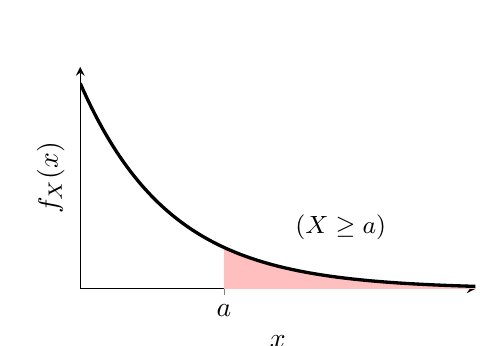
\begin{tikzpicture}
      \begin{axis}[
        width=6.6cm, height=4.4cm,
        axis lines=left,
        xlabel={$x$}, ylabel={$f_{X}(x)$},
        xmin=0, xmax=4.4, ymin=0, ymax=1.08,
        xtick={1.6}, xticklabels={$a$}, ytick=\empty,
        ]
        \addplot[name path=ft, domain=1.6:4.4, samples=60, draw=none] {exp(-x)};
        \addplot[name path=at, domain=1.6:4.4, samples=2, draw=none] {0};
        \addplot[fill=red!25] fill between[of=ft and at];
        \addplot[very thick, black, domain=0:4.4, samples=110] {exp(-x)};
        \node at (axis cs:2.9,0.30) {\small $\prob(X \geq a)$};
      \end{axis}
    \end{tikzpicture}

    {\small (a) the tail événement}
  \end{minipage}
  \hfill
  % right panel: a 1_{x>=a} <= x
  \begin{minipage}[b]{0.50\textwidth}
    \centering
    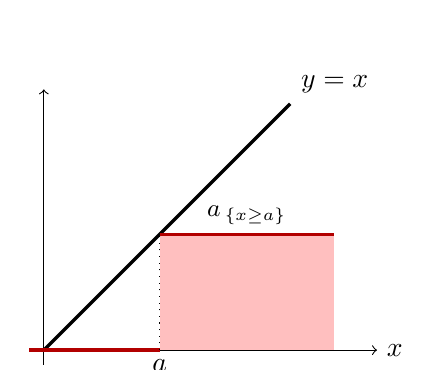
\begin{tikzpicture}[scale=0.92]
      \draw[->] (-0.2,0) -- (4.6,0) node[right] {$x$};
      \draw[->] (0,-0.2) -- (0,3.6);
      \fill[red!25] (1.6,0) rectangle (4.0,1.6);
      \draw[very thick, black] (0,0) -- (3.4,3.4) node[above right] {$y=x$};
      \draw[very thick, red!70!black] (-0.2,0) -- (1.6,0);
      \draw[very thick, red!70!black] (1.6,1.6) -- (4.0,1.6);
      \draw[dotted] (1.6,0) -- (1.6,1.6);
      \node[below] at (1.6,0) {$a$};
      \node[above] at (2.8,1.6) {\small $a\,\indic_{\{x \geq a\}}$};
    \end{tikzpicture}

    {\small (b) $a\,\indic_{\{X \geq a\}} \leq X$}
  \end{minipage}
  \caption{Inégalité de Markov. The rectangle of height $a$ over the tail sits
  under the line $y=x$, so taking espérances gives
  $a\,\prob(X \geq a) \leq \expec(X)$. The picture is the proof, and it is also
  where the hypothesis $X \geq 0$ enters: for negative $x$ the line dips below
  the axis and the domination fails.}
\end{figure}

\begin{prop}[Inégalité de Tchebychev (\textit{Tchebychev's inequality})]
  Soit $X$ une variable aléatoire réelle intégrable. Alors,
  \[
    \forall a > 0, \qquad \prob(|X - \expec(X)| \geq a) \leq \frac{\Var(X)}{a^{2}}.
  \]
\end{prop}

\begin{proof}
  Il suffit d'appliquer l'inégalité de Markov à la variable aléatoire
  $(X-\expec(X))^{2}$, which is non-negative as required, at the level
  $a^{2} > 0$ :
  \[
    \prob(|X-\expec(X)| \geq a)
      = \prob\big((X-\expec(X))^{2} \geq a^{2}\big)
      \leq \frac{\expec\big((X-\expec(X))^{2}\big)}{a^{2}}
      = \frac{\Var(X)}{a^{2}} .
  \]
  The first equality is the equivalence $|t| \geq a \iff t^{2} \geq a^{2}$ for
  $a>0$.
\end{proof}

Integrability of $X$ is what makes $\expec(X)$ exist, so that the statement can be
written at all; the bound is vacuously true when $\Var(X) = +\infty$ and carries
information only when the variance is finite. The shape $\Var(X)/a^{2}$ is the
reason Tchebychev, not Markov, gives the weak law of large numbers: applied to an
average of $n$ independent variables, the variance in the numerator carries a
factor $1/n$ and the bound goes to zero.

\begin{example}[A crude but universal bound on a Gaussian tail]
  Soit $X \sim \mathcal{N}(0,1)$ une variable aléatoire suivant une loi normale
  centrée réduite, so $\expec(X)=0$ and $\Var(X)=1$. Alors,
  \[
    \forall a > 0, \qquad \prob(|X| \geq a) \leq \frac{1}{a^{2}} .
  \]
  At $a=3$ this gives $\tfrac19 \approx 0.111$ against the true value
  $\approx 0.0027$: Tchebychev is far from sharp for a loi gaussienne, because it
  uses only two moments. Its value is that it uses only two moments.
\end{example}

\begin{example}[Comparing the two bounds on a Poisson tail]
  Soit $X \sim \mathcal{P}(\lambda)$ une variable aléatoire suivant une loi de
  Poisson, so $\expec(X)=\Var(X)=\lambda$, and fix $x > \lambda$. Markov,
  applicable because $X \geq 0$, gives
  \[
    \prob(X > x) \leq \frac{\lambda}{x} .
  \]
  Tchebychev, noting that $X > x$ implies $|X-\lambda| > x-\lambda > 0$, gives
  \[
    \prob(X > x) \leq \prob(|X-\lambda| \geq x-\lambda) \leq \frac{\lambda}{(x-\lambda)^{2}} .
  \]
  La seconde borne est meilleure si et seulement si $(x-\lambda)^{2} > x$, that is
  far out in the tail; close above $\lambda$ the first wins, and the Tchebychev
  bound even exceeds $1$ there. Neither is sharp --- the true tail decays
  super-exponentially --- and obtaining that decay needs Markov applied to
  $e^{\theta X}$ instead.
\end{example}

\begin{theorem}[Inégalité de Jensen (\textit{Jensen's inequality})]
  Soit $X$ une variable aléatoire réelle intégrable. Pour toute fonction convexe
  $\phi : \reals \to \reals$,
  \[
    \phi(\expec(X)) \leq \expec(\phi(X)).
  \]
\end{theorem}

\begin{proof}
  Comme la fonction $\phi$ est convexe, it lies above each of its supporting
  lines: il existe pour tout $a \in \reals$ un réel $\alpha$ tel que :
  \[
    \forall x \in \reals, \qquad \phi(x) - \phi(a) \geq \alpha(x-a).
  \]
  On choisit $a = \expec(X)$, which is finite because $X$ is integrable, et on
  applique l'inégalité à la variable aléatoire $X$, ce qui donne :
  \[
    \phi(X) - \phi(\expec(X)) \geq \alpha (X - \expec(X)).
  \]
  En passant à l'espérance, on obtient le résultat voulu, the right-hand side
  having espérance zero. Il faut juste s'assurer que la variable aléatoire
  $\phi(X)$ a bien une espérance, which is what the displayed inequality also
  delivers. Or l'inégalité implique que :
  \[
    \phi(X)^{-} \leq \big(\phi(\expec(X)) + \alpha(X-\expec(X))\big)^{-}
      \leq |\phi(\expec(X))| + |\alpha||X| + |\alpha||\expec(X)| ,
  \]
  whose espérance is finite by integrability of $X$. Donc
  $\expec(\phi(X)^{-}) < \infty$, ce qui implique que la variable aléatoire
  $\phi(X)$ a une espérance, and the inequality above may be integrated.
\end{proof}

The last paragraph of that proof is the part most often skipped and the part
worth keeping: Jensen asserts an inequality between two quantities, and one of
them has to be shown to exist before the assertion means anything. The mechanism
--- bound the negative part by an affine function of $|X|$, then use integrability
of $X$ --- is the same one used whenever an espérance must be shown to be well
defined. Note also that $\expec(\phi(X))$ may be $+\infty$, and the inequality
is then trivially true.

\begin{corollary}
  Soit $n$ un entier non nul. Pour tout vecteur aléatoire $X$ à valeurs dans
  $\reals^{n}$ et toute norme $\|\cdot\|$ de $\reals^{n}$,
  \[
    \|\expec(X)\| \leq \expec(\|X\|).
  \]
\end{corollary}

\begin{proof}
  Every norm is convex, par l'inégalité triangulaire and absolute homogeneity:
  $\|tx + (1-t)y\| \leq t\|x\| + (1-t)\|y\|$ for $t \in [0,1]$. C'est une
  conséquence de l'inégalité de Jensen, applied to $\phi = \|\cdot\|$ in its
  $\reals^{n}$-valued form, with the supporting line replaced by a supporting
  hyperplane.
\end{proof}

This corollary is the probabilistic triangle inequality, and it is used whenever
an espérance has to be moved inside a norm --- for instance to bound
$\|\expec(X) - \expec(Y)\|$ by $\expec(\|X-Y\|)$.

\begin{example}[The mean and the median are within one écart type]
  Soit $X$ une variable aléatoire réelle dont la fonction de répartition est
  continue, dérivable et strictement croissante, with finite espérance and finite
  variance. On appelle médiane l'unique réel $m$ tel que $F(m) = \tfrac12$. Then
  \[
    |\expec(X) - m| = |\expec(X-m)| \leq \expec(|X-m|) \leq \expec(|X - \expec(X)|)
      \leq \sqrt{\expec\big((X-\expec(X))^{2}\big)} = \sqrt{\Var(X)} .
  \]
  Three steps, the outer two Jensen. The first is Jensen for the absolute value.
  The second is the characterisation of the median as the minimiser of
  $a \mapsto \expec(|X-a|)$, applied at $a = \expec(X)$; that characterisation is
  a minimisation argument in its own right, not a convexity inequality, and it is
  taken here on trust. The third is Jensen for the square, in the form
  $\expec(|Z|)^{2} \leq \expec(Z^{2})$ --- which is also the inégalité de
  Cauchy-Schwartz against the constant $1$. So the mean and the median can never
  be more than one écart type apart, for every loi satisfying the hypotheses
  above.
\end{example}

\begin{conclusion}
  The chapter is chapters 2 and 3 with the total mass set to $1$, and most of
  what is stated above is one of their results transcribed. What is genuinely
  new is the vocabulary and the four things below.\\

  The loi $\prob_{X}$ is the only object a computation ever needs, and the
  théorème de transfert is what licenses that: an espérance written over the
  abstract $\Omega$ is an integral over the value space against $\prob_{X}$, so
  $\Omega$ can be left unnamed. A real loi is then read through its fonction de
  répartition, whose jumps are its atoms, or through a densité with respect to
  the mesure de Lebesgue --- which exists only under a condition strictly
  stronger than continuity of $F_{X}$, the devil's staircase being the
  counter-example that fixes how much stronger.\\

  The fonction test method is the calculation the written papers ask for most
  often. To find the densité of $Y = g(X)$: take an arbitrary non-negative
  mesurable $\phi$, expand $\expec(\phi(Y))$ by transfer, change variables
  until $\phi$ is evaluated at the integration variable and nothing else depends
  on it, then read the densité off. It needs no monotonicity and no
  invertibility of $g$, it works in the vector case where there is no fonction de
  répartition worth differentiating, and when it fails it fails informatively: a
  term surviving in $\phi(x_{0})$ is an atom at $x_{0}$ of exactly that mass.\\

  The bilinearity of the covariance is the identity the limit theorems run on.
  In scalar form $\Var(X+Y) = \Var(X) + 2\Cov(X,Y) + \Var(Y)$; in vector form
  $\Cov(X+Y) = \Cov(X) + \Cov(Y) + \Cov(X,Y) + \Cov(X,Y)^{T}$, where the two
  cross terms are transposes and cannot be merged. Under indépendance both
  vanish, so $n$ independent variables of common variance $\sigma^{2}$ give
  $\Var(X_{1}+\dots+X_{n}) = n\sigma^{2}$ and an écart type of order
  $\sqrt{n}$, which is the normalisation chapter 8 divides by. Zero covariance
  is strictly weaker than indépendance, and the uniform variable against its own
  square is the standing reminder.\\

  The inequalities are what turn a moment into a tail bound: Markov for a
  non-negative variable, Tchebychev for its second-moment consequence, Jensen
  for a convex function of an integrable variable. Jensen's proof carries the
  step usually skipped --- showing that $\expec(\phi(X))$ exists before asserting
  an inequality about it --- and that argument, bounding a negative part by an
  affine function of $|X|$, is reusable wherever an espérance has to be shown
  to be well defined.
\end{conclusion}

\section{Loi conditionnelle}

Conditioning is the operation of revising a loi once part of the outcome is
known. In the discrete chapter it was an elementary quotient: the probabilité
conditionnelle of $B$ given $A$ was $\prob(A \intersect B)/\prob(A)$, and nothing
more was needed because the événements one conditions on are atoms with positive
probability. The moment variables aléatoires have densités that quotient breaks
down. The événement $\{Y = y\}$ is négligeable for every $y$, its probability is
zero, and the quotient is $0/0$; yet everyone wants to speak of the loi of $X$
given $Y = y$, and every exam problem in this course asks for one.\\

This chapter builds the object that survives the degeneracy. The route is the
one the intégrale de Lebesgue makes available: instead of dividing by
$\prob(Y = y)$, one observes that the map $B \mapsto \prob_{X,Y}(A \times B)$ is
dominated by $\prob_{Y}$, so by the théorème de Radon-Nikodym it has a densité with
respect to $\prob_{Y}$, and that densité --- read as a function of $y$ --- is
declared to be the loi conditionnelle. The price of the construction is a
qualification that never goes away: the loi conditionnelle exists and is determined
only for $\prob_{Y}$-almost every $y$. That qualification is not decoration, and it
is the reason the statements below are all phrased with an ``almost every''.\\

The plan is three steps of increasing generality: conditioning on a single
événement non négligeable, which is chapter 1 re-read with an integral in place of a
sum; conditioning on a variable aléatoire, where the loi conditionnelle appears as a
densité with respect to $\prob_{Y}$; and the case where the loi jointe has a
densité, which is the computational case the exercises live in. Espérance
conditionnelle follows, defined as an integral against the loi conditionnelle, and the
chapter closes on the tower property $\expec(X) = \expec(\expec(X \mid Y))$ with
its proof, the standard four-rung ladder of the course.

\begin{remark}
  This course builds espérance conditionnelle \emph{from} lois
  conditionnelles: $\expec(\phi(X,Y) \mid Y = y)$ is by definition an integral
  of $\phi(\cdot,y)$ against the mesure $\prob_{X \mid Y = y}$. Other
  treatments define espérance conditionnelle abstractly rather than from
  lois conditionnelles; that route is not taken here, and nothing below depends
  on it.
\end{remark}

\subsection{Condition sur un événement non négligeable}

On commence par le cas simple où la condition porte sur un événement de
probabilité non nulle. Soit $(\Omega,\mathcal{F},\prob)$ un espace de probabilité et
$A \in \mathcal{F}$ un événement tel que :
\[
  \prob(A) > 0 .
\]
La probabilité conditionnelle $\prob(\cdot \mid A)$ définit une nouvelle mesure de
probabilité sur $(\Omega,\mathcal{F})$, the same espace mesurable :
\[
  \forall B \in \mathcal{F}, \qquad
  \prob(B \mid A) \;=\; \frac{\prob(A \intersect B)}{\prob(A)}
  \;=\; \int_{B} \frac{\indic_{A}}{\prob(A)} \, d\prob .
\]
The second form is the one that generalises. It says, of
$\prob(\cdot \mid A)$ : c'est une mesure de densité
\begin{equation*}
  \omega \longmapsto \frac{\indic_{A}(\omega)}{\prob(A)} ,
\end{equation*}
par rapport à $\prob$, and everything in this subsection is a consequence of that
single sentence read through the results of chapter 3 on mesures à densité.\\

Soit $X$ une variable aléatoire à valeurs dans un espace mesurable
$(E,\mathcal{E})$ --- not necessarily real, at this stage.

\begin{definition}[Loi conditionnelle sachant un événement]
  On appelle loi conditionnelle de $X$ sachant $A$ la mesure de probabilité
  $\prob_{X \mid A}$ sur $(E,\mathcal{E})$ définie par :
  \[
    \forall B \in \mathcal{E}, \qquad
    \prob_{X \mid A}(B) \;=\; \prob(X \in B \mid A) .
  \]
\end{definition}

C'est la mesure image de la probabilité conditionnelle
$\prob(\cdot \mid A)$ par $X$, in exactly the sense chapter 4 gives to the loi
$\prob_{X}$ of a variable aléatoire: replace the mesure upstairs by
$\prob(\cdot \mid A)$ and push it forward through $X$. In particular
$\prob_{X \mid A}$ is a mesure de probabilité on $(E,\mathcal{E})$ with no further
verification needed, since the image of a mesure de probabilité is a mesure de
probabilité.\\

On suppose maintenant que $X$ est à valeurs réelles, for the rest of this
subsection, so that an espérance can be spoken of.

\begin{definition}[Espérance conditionnelle sachant un événement]
  On appelle espérance conditionnelle de la variable aléatoire $X$ sachant $A$
  la valeur :
  \[
    \expec(X \mid A) \;=\; \int X(\omega) \, d\prob(\omega \mid A),
  \]
  dès que cette intégrale est bien définie.
\end{definition}

The caveat ``dès que cette intégrale est bien définie'' is the chapter 3 caveat and
is not a formality: it excludes the case
$\int X^{+} \, d\prob(\cdot \mid A) = \int X^{-} \, d\prob(\cdot \mid A) = +\infty$,
where no value can be assigned. C'est l'espérance de $X$ pour la probabilité
conditionnelle $\prob(\cdot \mid A)$, rather than for $\prob$. D'après le théorème de
transfert, which applies verbatim, on l'obtient directement à partir de la loi
conditionnelle :
\begin{equation*}
  \expec(X \mid A) \;=\; \int x \, d\prob_{X \mid A}(x) .
\end{equation*}

\begin{prop}[Espérance conditionnelle comme quotient]
  L'espérance conditionnelle de la variable aléatoire $X$ sachant $A$ vérifie :
  \[
    \expec(X \mid A) \;=\; \frac{\expec(X \indic_{A})}{\prob(A)} .
  \]
\end{prop}

The proof is the densité in one line. Integrating against a mesure that has
densité $\indic_{A}/\prob(A)$ with respect to $\prob$ is the same as integrating
against $\prob$ after multiplying by that densité, so
\[
  \expec(X \mid A)
  \;=\; \int X(\omega) \, d\prob(\omega \mid A)
  \;=\; \int X(\omega) \frac{\indic_{A}(\omega)}{\prob(A)} \, d\prob(\omega)
  \;=\; \frac{\expec(X \indic_{A})}{\prob(A)} .
\]
The step in the middle is the chapter 3 rule for integrating against a mesure
given by a densité, and it holds as soon as one of the two integrals is well
defined.\\

On en déduit l'équivalent de la formule des probabilités totales pour l'espérance.

\begin{prop}[Équivalent de la formule des probabilités totales pour l'espérance]
  Soit $(A_{i})_{i \in I}$ une famille d'événements formant une partition de
  $\Omega$, avec $\prob(A_{i}) > 0$ pour tout $i \in I$. Alors,
  \[
    \expec(X) \;=\; \sum_{i \in I} \prob(A_{i}) \expec(X \mid A_{i})
  \]
  dès que la variable aléatoire $X$ est positive ou intégrable.
\end{prop}

Comme $\sum_{i \in I} \indic_{A_{i}} = 1$ --- a partition writes the constant $1$
that way --- one has $X = \sum_{i \in I} X \indic_{A_{i}}$ pointwise. Exchanging the
espérance with the sum is legitimate exactly under the stated hypothesis --- the
chapter 4 result on the espérance of a series asks for the terms to be positive, or
for the series of the espérances of the absolute values to converge --- and then
each term is rewritten with the previous proposition:
\[
  \expec(X) \;=\; \sum_{i \in I} \expec(X \indic_{A_{i}})
             \;=\; \sum_{i \in I} \prob(A_{i}) \expec(X \mid A_{i}) .
\]

\begin{remark}
  One hypothesis genuinely carries weight: $X$ must be positive or integrable,
  since otherwise the exchange of espérance and sum has no justification and
  the right-hand side can fail to mean anything. Countability of the index set
  $I$ is \emph{not} an extra assumption --- a partition of $\Omega$ into événements
  of strictly positive probability is automatically at most countable, since for
  each $n$ only finitely many of them can have probability above $1/n$. That is
  what makes the chapter 4 result on the espérance of a \emph{series}
  applicable in the first place.
\end{remark}

\begin{example}[Splitting an espérance over the value of a first draw]
  A box holds two coins, one fair and one biased with $\prob(\text{heads}) = 3/4$.
  A coin is drawn uniformly and tossed $n$ times; let $X$ be the number of heads,
  $A_{1}$ the événement that the fair coin was drawn and $A_{2} = A_{1}^{c}$. Given
  $A_{1}$ the variable $X$ has loi $\mathcal{B}(n,1/2)$, given $A_{2}$ it has loi
  $\mathcal{B}(n,3/4)$, and the formule des probabilités totales pour l'espérance
  gives
  \[
    \expec(X) \;=\; \tfrac{1}{2} \cdot \tfrac{n}{2} + \tfrac{1}{2} \cdot \tfrac{3n}{4}
              \;=\; \tfrac{5n}{8} .
  \]
  Nothing here needs the machinery of the rest of the chapter: the conditioning
  événements have positive probability. This is the situation that generalises badly,
  and the next subsection is about what replaces it.
\end{example}

\subsection{Condition sur une variable aléatoire}

On considère maintenant deux variables aléatoires $X$ et $Y$ à valeurs dans les
espaces mesurables respectifs $(\reals,\mathcal{B}(\reals))$ et $(E,\mathcal{E})$.
Les résultats s'étendent au cas où $X$ est un vecteur aléatoire, à valeurs dans
$(\reals^{n},\mathcal{B}(\reals^{n}))$, without change; only the notation gets
heavier. On souhaite définir la loi conditionnelle de $X$ sachant $Y = y$, pour une
certaine valeur $y \in E$, \emph{même si l'événement associé, $\{Y = y\}$, est de
probabilité nulle}.

\begin{example}[The smaller of two uniform draws, given the larger]
  Soit $X = \min(U,V)$ et $Y = \max(U,V)$, avec $U$, $V$ des variables aléatoires
  i.i.d.\ de loi uniforme sur $[0,1]$. L'événement $\{Y = \tfrac{1}{2}\}$ est de
  probabilité nulle, so no quotient defines a loi of $X$ given it. Nevertheless
  there is an answer, and it is the one intuition expects: la loi conditionnelle de
  $X$ sachant $Y = \tfrac{1}{2}$ est une loi uniforme sur $[0,\tfrac{1}{2}]$. The
  rest of this chapter is what makes that sentence mean something, and the
  computation appears in the next subsection.
\end{example}

\begin{remark}
  Lorsque $Y = \indic_{A}$ et $y = 1$, où $A \in \mathcal{F}$ est un événement non
  négligeable, on retrouve le cas considéré précédemment. The construction below
  must --- and will --- agree with the previous subsection on that overlap.
\end{remark}

The observation that unlocks everything is a comparison of masses. For every
borélien $A$ and every $B \in \mathcal{E}$,
\[
  \prob_{X,Y}(A \times B) \;=\; \prob(X \in A, \, Y \in B)
  \;\leq\; \prob(Y \in B) \;=\; \prob_{Y}(B) .
\]
Fix the borélien $A$ and read this as a statement about the set function
$B \mapsto \prob_{X,Y}(A \times B)$ on $(E,\mathcal{E})$: it is a mesure, and it
vanishes on every $B$ with $\prob_{Y}(B) = 0$. It is therefore absolument continue
par rapport à la mesure $\prob_{Y}$, et ce quel que soit le borélien $A$. Both
mesures are finite --- they are bounded by $1$ --- hence $\sigma$-finies, which is
the hypothesis the théorème de Radon-Nikodym of chapter 3 requires. Par le théorème
de Radon-Nikodym, la mesure $B \mapsto \prob_{X,Y}(A \times B)$ admet une densité
par rapport à la mesure $\prob_{Y}$, que l'on définit comme la loi conditionnelle de
$X$ par rapport à $Y$. Because a densité is determined only up to a négligeable
set, and the relevant négligeable sets here are the $\prob_{Y}$-négligeable ones,
elle est unique à un ensemble négligeable près pour la mesure $\prob_{Y}$.

\begin{definition}[Loi conditionnelle sachant une variable aléatoire]
  Pour $\prob_{Y}$-presque tout $y$, on définit la loi conditionnelle de $X$ sachant
  $Y = y$ comme une mesure de probabilité sur
  $(\reals,\mathcal{B}(\reals))$, notée $\prob_{X \mid Y = y}$, telle que :
  \[
    \forall A \in \mathcal{B}(\reals), \;\; \forall B \in \mathcal{E}, \qquad
    \prob_{X,Y}(A \times B) \;=\; \int_{B} \prob_{X \mid Y = y}(A) \, d\prob_{Y}(y) .
  \]
\end{definition}

\begin{remark}
  The ``$\prob_{Y}$-presque tout $y$'' is not a technical nicety that a careful
  reader may drop. The loi conditionnelle is defined by an integral identity that
  must hold for every borélien $A$: elle est définie à un ensemble négligeable près
  --- a $\prob_{Y}$-négligeable exceptional set --- qui dépend du borélien $A$
  considéré. Nothing in the théorème de Radon-Nikodym says these exceptional sets
  can be chosen inside a single négligeable set, uniformly in $A$, and there are
  uncountably many $A$ to union over. So l'existence d'une telle mesure
  $\prob_{X \mid Y = y}$ --- one that works simultaneously for all $A$, for
  $\prob_{Y}$-almost every $y$ --- n'est pas immédiate: it is a genuine theorem and
  not a corollary. C'est le \textbf{théorème de Jirina} (\textit{Jirina's theorem}),
  which this course states and does not prove.
\end{remark}

\begin{prop}[La loi conditionnelle est une mesure de probabilité]
  Pour $\prob_{Y}$-presque tout $y$, $\prob_{X \mid Y = y}$ est une mesure de
  probabilité.
\end{prop}

Both defining properties are checked by the p.p.\ uniqueness of a densité, the
chapter 3 statement that two positive mesurable functions integrating to the
same value on every mesurable set are equal $\nu$-p.p.\ when $\nu$ is
$\sigma$-finie --- and $\prob_{Y}$, being a mesure de probabilité, is. For the
total mass, take $A = \reals$:
\[
  \forall B \in \mathcal{E}, \qquad
  \prob_{X,Y}(\reals \times B) \;=\; \int_{B} \prob_{X \mid Y = y}(\reals) \, d\prob_{Y}(y)
  \;=\; \int_{B} d\prob_{Y}(y) ,
\]
the last equality because $\prob_{X,Y}(\reals \times B) = \prob_{Y}(B)$. Uniqueness
applies, ce qui montre que $\prob_{X \mid Y = y}(\reals) = 1$ pour
$\prob_{Y}$-presque tout $y$. For countable additivity: pour toute famille au plus
dénombrable de boréliens deux-à-deux disjoints $(A_{i})_{i \in I}$,
\begin{align*}
  \forall B \in \mathcal{E}, \qquad
  \prob_{X,Y}\Big( \bigcup_{i \in I} A_{i} \times B \Big)
  &= \sum_{i \in I} \prob_{X,Y}(A_{i} \times B) \\
  &= \sum_{i \in I} \int_{B} \prob_{X \mid Y = y}(A_{i}) \, d\prob_{Y}(y) \\
  &= \int_{B} \sum_{i \in I} \prob_{X \mid Y = y}(A_{i}) \, d\prob_{Y}(y) ,
\end{align*}
the exchange of sum and integral being legitimate because the terms are positive.
Uniqueness applies again, ce qui montre que
$\prob_{X \mid Y = y}(\union_{i \in I} A_{i}) = \sum_{i \in I} \prob_{X \mid Y = y}(A_{i})$
pour $\prob_{Y}$-presque tout $y$.

\begin{remark}
  Notice that the exceptional set produced by this argument depends on the family
  $(A_{i})$ chosen. This is exactly the difficulty the previous remark described,
  and exactly what the théorème de Jirina repairs.
\end{remark}

On vérifie que la définition coïncide avec celle vue précédemment, lorsque la
condition porte sur un événement $A \in \mathcal{F}$ de probabilité non nulle,
$\prob(A) > 0$. En prenant $Y = \indic_{A}$, so that $E$ is $\{0,1\}$ and
$\prob_{Y}(\{1\}) = \prob(A) > 0$, and $B = \{1\}$ in the defining identity, on
obtient :
\[
  \forall B' \in \mathcal{B}(\reals), \qquad
  \prob_{X,Y}(B' \times \{1\}) \;=\; \prob_{X \mid Y = 1}(B') \, \prob_{Y}(\{1\}) ,
\]
si bien que :
\[
  \forall B' \in \mathcal{B}(\reals), \qquad
  \prob_{X \mid Y = 1}(B') \;=\; \frac{\prob(X \in B', \, Y = 1)}{\prob(Y = 1)}
  \;=\; \prob(X \in B' \mid A) .
\]
The new loi conditionnelle is the old one. Note that here the ``presque tout $y$''
costs nothing: $E$ has two points, both of positive mass when $\prob(A) \in (0,1)$,
so ``$\prob_{Y}$-presque tout $y$'' means every $y$.

\begin{prop}[Loi jointe]
  La loi jointe des variables aléatoires $X$ et $Y$ vérifie :
  \[
    \forall C \in \mathcal{B}(\reals) \otimes \mathcal{E}, \qquad
    \prob_{X,Y}(C) \;=\; \int \left( \int \indic_{C}(x,y) \, d\prob_{X \mid Y = y}(x) \right) d\prob_{Y}(y) .
  \]
\end{prop}

L'égalité est vérifiée pour tout ensemble produit $C = A \times B$ par définition
--- the definition of the loi conditionnelle, and nothing else. The extension to
the whole tribu produit is the théorème d'unicité of chapter 2: the two sides are
mesures de probabilité on $\mathcal{B}(\reals) \otimes \mathcal{E}$, they agree on
the collection of product sets $A \times B$, that collection is stable par
intersection finie --- the intersection of two rectangles is a rectangle --- it
generates the tribu produit by definition, and $\reals \times E$ is itself a
rectangle of finite mesure, so the covering condition holds. Hence the two mesures
coincide everywhere.

\begin{remark}
  This proposition is the one to keep in mind, because it is the statement that
  a loi jointe \emph{factorises}. A pair $(X,Y)$ can be specified in two stages:
  give the loi marginale $\prob_{Y}$, then give, for $\prob_{Y}$-almost every $y$,
  a loi conditionnelle $\prob_{X \mid Y = y}$. The proposition says that these two
  ingredients determine $\prob_{X,Y}$ completely. Almost every model in the
  exercises is written this way --- ``$Y$ is exponential, and given $Y = y$ the
  variable $X$ is Poisson of parameter $y$'' --- and the proposition is what turns
  such a sentence into a loi jointe one can integrate against.
\end{remark}

\begin{figure}[h!]
  \centering
  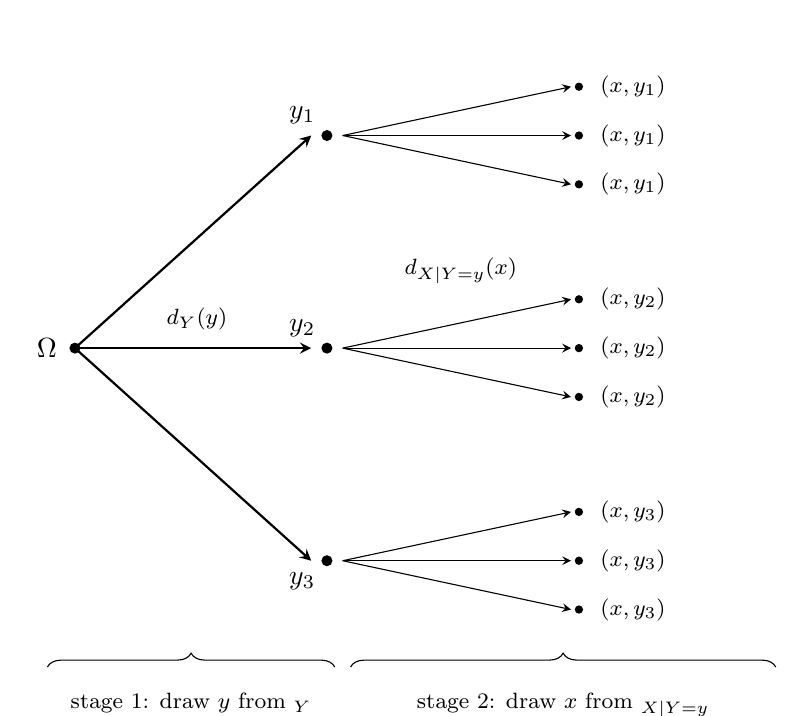
\begin{tikzpicture}[>=stealth, scale=1.0]
    % stage one
    \fill (0,0) circle (2pt) node[left=3pt] {$\Omega$};
    \draw[->, thick] (0,0) -- (3.0,2.7);
    \draw[->, thick] (0,0) -- (3.0,0.0);
    \draw[->, thick] (0,0) -- (3.0,-2.7);
    \node[above] at (1.55,0.1) {\footnotesize $d\prob_{Y}(y)$};
    \fill (3.2,2.7) circle (2pt) node[above left=1pt] {$y_{1}$};
    \fill (3.2,0.0) circle (2pt) node[above left=1pt] {$y_{2}$};
    \fill (3.2,-2.7) circle (2pt) node[below left=1pt] {$y_{3}$};
    % stage two
    \foreach \yy in {2.7,0.0,-2.7} {
      \draw[->] (3.4,\yy) -- (6.3,\yy+0.62);
      \draw[->] (3.4,\yy) -- (6.3,\yy);
      \draw[->] (3.4,\yy) -- (6.3,\yy-0.62);
      \fill (6.4,\yy+0.62) circle (1.5pt);
      \fill (6.4,\yy) circle (1.5pt);
      \fill (6.4,\yy-0.62) circle (1.5pt);
    }
    \foreach \yy/\lab in {2.7/1, 0.0/2, -2.7/3} {
      \node[right] at (6.55,\yy+0.62) {\footnotesize $(x,y_{\lab})$};
      \node[right] at (6.55,\yy) {\footnotesize $(x,y_{\lab})$};
      \node[right] at (6.55,\yy-0.62) {\footnotesize $(x,y_{\lab})$};
    }
    \node[above] at (4.9,0.7) {\footnotesize $d\prob_{X \mid Y = y}(x)$};
    % braces
    \draw[decorate, decoration={brace, amplitude=5pt}] (-0.35,-4.05) -- (3.3,-4.05)
      node[midway, below=6pt] {\footnotesize stage 1: draw $y$ from $\prob_{Y}$};
    \draw[decorate, decoration={brace, amplitude=5pt}] (3.5,-4.05) -- (8.9,-4.05)
      node[midway, below=6pt] {\footnotesize stage 2: draw $x$ from $\prob_{X \mid Y = y}$};
  \end{tikzpicture}
\end{figure}

The tree is the picture of the proposition. A point is produced in two stages,
and the probability of a set $C$ is obtained by integrating, over the first
stage, the probabilité conditionnelle computed at the second --- which with
$\phi = \indic_{C}$ is the displayed identity, and with a general $\phi$ is
the tower property of the last subsection.

\begin{prop}[Indépendance]
  Les variables aléatoires $X$ et $Y$ sont indépendantes si et seulement si la loi
  conditionnelle de $X$ sachant $Y = y$ est la loi de $X$ pour $\prob_{Y}$-presque
  tout $y$.
\end{prop}

Les variables aléatoires $X$ et $Y$ sont indépendantes si et seulement si
$\prob_{X,Y}(A \times B) = \prob_{X}(A) \prob_{Y}(B)$ for every borélien $A$ and every
$B \in \mathcal{E}$, ce qui est équivalent --- by the definition of the loi
conditionnelle --- à :
\[
  \forall A \in \mathcal{B}(\reals), \;\; \forall B \in \mathcal{E}, \qquad
  \int_{B} \prob_{X \mid Y = y}(A) \, d\prob_{Y}(y) \;=\; \int_{B} \prob_{X}(A) \, d\prob_{Y}(y) ,
\]
and p.p.\ uniqueness of densités turns the equality of the integrals into
$\prob_{X \mid Y = y}(A) = \prob_{X}(A)$ for $\prob_{Y}$-almost every $y$. So
indépendance is exactly the statement that conditioning on $Y$ teaches nothing
about $X$.

\begin{prop}[Condition sur une variable qui détermine l'autre]
  Si $X = \phi(Y)$ pour une certaine fonction mesurable $\phi$, alors la loi
  conditionnelle de $X$ sachant $Y = y$ est la mesure de Dirac en $\phi(y)$ pour
  $\prob_{Y}$-presque tout $y$.
\end{prop}

Indeed, for every borélien $A$ and every $B \in \mathcal{E}$,
\[
  \prob_{X,Y}(A \times B) \;=\; \prob(\phi(Y) \in A, \, Y \in B)
  \;=\; \int_{B} \indic_{A}(\phi(y)) \, d\prob_{Y}(y) ,
\]
on en déduit que pour $\prob_{Y}$-presque tout $y$,
$\prob_{X \mid Y = y}(A) = \indic_{A}(\phi(y)) = \delta_{\phi(y)}(A)$. The two
propositions are the two extremes of the same scale: knowing $Y$ tells nothing
about $X$ (indépendance, the loi conditionnelle is the unconditional one), or
knowing $Y$ tells everything (the loi conditionnelle is a point mass).

\begin{example}[The square of a uniform variable, given the variable]
  Soit $X$ une variable aléatoire de loi uniforme sur $[0,1]$. Pour presque tout
  $x \in [0,1]$, la loi conditionnelle de $X^{2}$ sachant $X = x$ est une mesure de
  Dirac en $x^{2}$. There is no randomness left to describe once $X$ is known, and
  the loi conditionnelle records that by collapsing to a point.
\end{example}

\subsection{Cas des lois à densité}

The general construction is not a recipe. It becomes one as soon as the loi jointe
has a densité, and that is the situation of every computation in this course.
On considère maintenant le cas de variables aléatoires réelles $X$, $Y$ dont la loi
jointe a une densité $f_{X,Y}$ par rapport à la mesure de Lebesgue de $\reals^{2}$.
Les variables aléatoires $X$ et $Y$ ont donc des densités par rapport à la mesure de
Lebesgue sur $\reals$, each obtained as usual by integrating out the other variable.

\begin{definition}[Densité conditionnelle]
  Pour tout réel $y$ tel que $f_{Y}(y) > 0$, on définit la \textbf{densité
  conditionnelle} (\textit{conditional density}) de la variable aléatoire $X$ par
  rapport à $Y = y$ comme la fonction $f_{X \mid Y = y}$ définie par :
  \[
    \forall x \in \reals, \qquad
    f_{X \mid Y = y}(x) \;=\; \frac{f_{X,Y}(x,y)}{f_{Y}(y)} .
  \]
\end{definition}

The condition $f_{Y}(y) > 0$ is part of the definition and not a side remark: at a
$y$ where the marginal densité vanishes the quotient is $0/0$ and no densité
conditionnelle is defined there. This is the trace, at the level of densités, of the
``$\prob_{Y}$-presque tout $y$'' of the previous subsection, since
$\{f_{Y} = 0\}$ carries no $\prob_{Y}$-mass. On vérifie que la loi conditionnelle a
bien pour densité cette fonction par rapport à la mesure de Lebesgue --- a short
verification. For all $A, B \in \mathcal{B}(\reals)$,
\begin{align*}
  \prob_{X,Y}(A \times B)
  &= \int_{A \times B} f_{X,Y}(x,y) \, dx \, dy \\
  &= \int_{A \times B} f_{X \mid Y = y}(x) f_{Y}(y) \, dx \, dy \\
  &= \int_{B} \left( \int_{A} f_{X \mid Y = y}(x) \, dx \right) f_{Y}(y) \, dy ,
\end{align*}
where the middle line is legitimate because on $\{f_{Y} = 0\}$ one has
$\int f_{X,Y}(x,y) \, dx = f_{Y}(y) = 0$, so that set of $y$ contributes nothing
to either side of the identity, and the last line is Tonelli, applicable
because the integrand is positive. Comparing with the defining identity of the
loi conditionnelle gives, pour $\prob_{Y}$-presque tout $y$,
\[
  \forall A \in \mathcal{B}(\reals), \qquad
  \prob_{X \mid Y = y}(A) \;=\; \int_{A} f_{X \mid Y = y}(x) \, dx .
\]

\begin{remark}
  Two extensions come free and both are used constantly. Les résultats s'étendent
  sans difficulté au cas où la loi jointe a une densité par rapport à une mesure
  \emph{produit} quelconque, not only Lebesgue$\,\otimes\,$Lebesgue (par exemple, le
  produit de la mesure de Lebesgue sur $\reals$ et d'une mesure discrète --- the
  important case being the mesure de comptage
  $\mu = \sum_{n \in \mathbb{N}} \delta_{n}$ on $\mathbb{N}$, which is what one
  needs when one variable is discrete and the other continuous), ainsi qu'au cas où
  $X$ et $Y$ sont des vecteurs aléatoires. The formula
  $f_{X \mid Y = y} = f_{X,Y}/f_{Y}$ is unchanged in both cases; only the reference
  mesure changes, and with it the meaning of ``densité''.
\end{remark}

\begin{remark}
  A practical consequence: at fixed $y$, $f_{X \mid Y = y}$ is proportional to
  $f_{X,Y}(\cdot,y)$, the constant being whatever makes it integrate to $1$. So
  one writes $f_{X \mid Y = y}(x) \propto f_{X,Y}(x,y)$, recognises the shape of a
  standard loi in $x$, and reads its normalisation off a table rather than
  computing $f_{Y}$. Most solutions below are obtained this way.
\end{remark}

\begin{example}[The smaller of two uniform draws, given the larger]
  Return to $X = \min(U,V)$ and $Y = \max(U,V)$ with $U,V$ independent uniform on
  $[0,1]$. Pour toute fonction mesurable positive $\phi$ --- a fonction test ---
  \[
    \expec(\phi(X,Y)) = \int \phi(\min(u,v),\max(u,v)) \indic_{]0,1[}(u) \indic_{]0,1[}(v) \, du \, dv
    = 2 \int \phi(x,y) \indic_{\Delta}(x,y) \, dx \, dy
  \]
  avec $\Delta = \{(x,y) \in [0,1]^{2} : x \leq y\}$, the factor $2$ coming from
  the two orderings of the pair. So la loi jointe a pour densité :
  \[
    f_{X,Y}(x,y) \;=\; 2 \times \indic_{\Delta}(x,y) ,
  \]
  la loi de $Y$ a pour densité $f_{Y}(y) = 2y \indic_{[0,1]}(y)$, and for every
  $y \in \;]0,1]$
  \[
    f_{X \mid Y = y}(x) \;=\; \frac{\indic_{\Delta}(x,y)}{y} ,
  \]
  c'est une loi uniforme sur $[0,y]$. The guess made when the example was
  introduced is confirmed, and $y = 0$ --- the single point where $f_{Y}$ vanishes
  --- is excluded, as the definition requires.
\end{example}

\begin{figure}[h!]
  \centering
  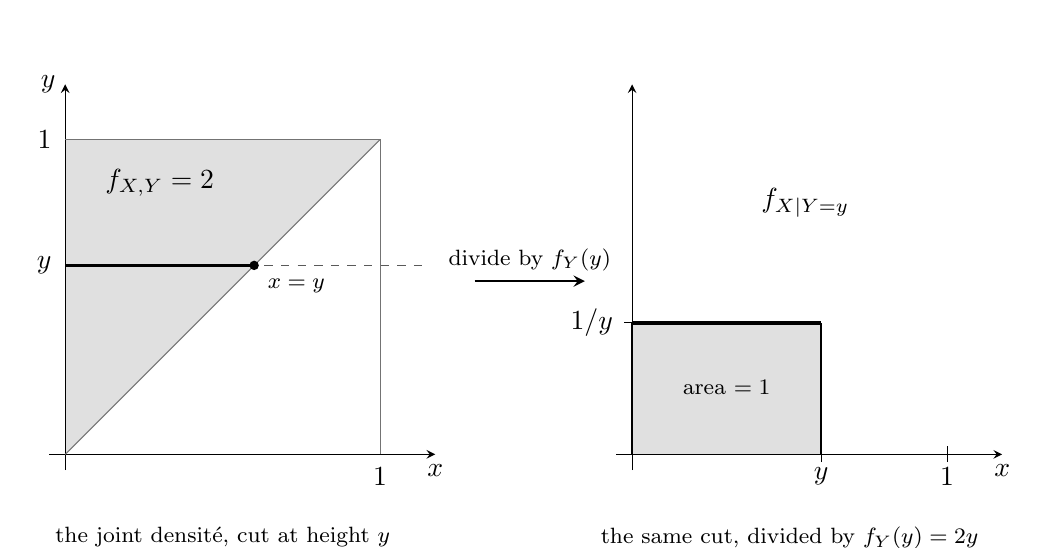
\begin{tikzpicture}[>=stealth, scale=1.0]
    % ---- left panel: the joint density on the triangle, sliced
    \fill[black!12] (0,0) -- (0,4) -- (4,4) -- cycle;
    \draw[->] (-0.2,0) -- (4.7,0) node[below] {$x$};
    \draw[->] (0,-0.2) -- (0,4.7) node[left] {$y$};
    \draw[thin,black!55] (0,0) -- (4,4);
    \draw[thin,black!55] (0,4) -- (4,4);
    \draw[thin,black!55] (4,0) -- (4,4);
    \node at (1.2,3.45) {$f_{X,Y} = 2$};
    \node[below] at (4,-0.05) {$1$};
    \node[left] at (-0.05,4) {$1$};
    % the slice
    \draw[dashed,black!65] (0,2.4) -- (4.6,2.4);
    \draw[very thick] (0,2.4) -- (2.4,2.4);
    \fill (2.4,2.4) circle (1.7pt);
    \node[left] at (-0.05,2.4) {$y$};
    \node[below right] at (2.45,2.35) {\footnotesize $x = y$};
    \node[below] at (2.0,-0.8) {\footnotesize the joint densité, cut at height $y$};
    % ---- right panel: the renormalised slice
    \begin{scope}[xshift=7.2cm]
      \draw[->] (-0.2,0) -- (4.7,0) node[below] {$x$};
      \draw[->] (0,-0.2) -- (0,4.7) node[left] {};
      \fill[black!12] (0,0) rectangle (2.4,1.67);
      \draw[very thick] (0,1.67) -- (2.4,1.67);
      \draw[thick] (0,0) -- (0,1.67);
      \draw[thick] (2.4,0) -- (2.4,1.67);
      \draw (-0.1,1.67) -- (0.1,1.67);
      \node[left] at (-0.12,1.67) {$1/y$};
      \draw (2.4,-0.1) -- (2.4,0.1);
      \node[below] at (2.4,-0.05) {$y$};
      \draw (4,-0.1) -- (4,0.1);
      \node[below] at (4.0,-0.05) {$1$};
      \node at (1.2,0.85) {\footnotesize area $= 1$};
      \node at (2.2,3.2) {$f_{X \mid Y = y}$};
      \node[below] at (2.0,-0.8) {\footnotesize the same cut, divided by $f_{Y}(y) = 2y$};
    \end{scope}
    % the arrow between panels
    \draw[->, thick] (5.2,2.2) -- (6.6,2.2)
      node[midway,above] {\footnotesize divide by $f_{Y}(y)$};
  \end{tikzpicture}
\end{figure}

The figure is the whole of this subsection in one image. Conditioning on
$Y = y$ means cutting the joint densité along the horizontal line at height $y$
and reading the profile of the cut as a function of $x$; that profile is
$f_{X,Y}(\cdot,y)$, not a probability densité, since it integrates to $f_{Y}(y)$
rather than $1$. Dividing by $f_{Y}(y)$ renormalises it. The picture also makes
the restriction $f_{Y}(y) > 0$ visible: where the cut meets the support in a set
of mesure zero there is nothing to renormalise.

\begin{prop}[Indépendance pour un couple à densité]
  Deux variables aléatoires $X, Y$ dont la loi jointe a une densité sont
  indépendantes si et seulement si la densité conditionnelle $f_{X \mid Y = y}$ est
  égale à la densité $f_{X}$, pour tout $y$ tel que $f_{Y}(y) > 0$.
\end{prop}

By the chapter 4 criterion, a pair with a joint densité is independent if and
only if $f_{X,Y}(x,y) = f_{X}(x) f_{Y}(y)$ p.p., which is to say
\[
  f_{X \mid Y = y}(x) f_{Y}(y) \;=\; f_{X}(x) f_{Y}(y)
\]
for Lebesgue-almost every $x$, at almost every $y$ with $f_{Y}(y) > 0$. Dividing by
$f_{Y}(y)$, which is legitimate exactly on that set of $y$, gives the claim.
A densité is only defined up to a set of mesure zero, so ``pour tout $y$'' is
to be read for a suitable choice of the densities; for an arbitrary choice the
equality holds p.p.\ in $y$ on the set where $f_{Y}(y) > 0$.

\begin{example}[A point drawn uniformly in the unit disc]
  Soit $A$ un point choisi de manière aléatoire et uniforme dans le disque unité
  $D$, centred at the origin. On note $(X,Y)$ ses coordonnées cartésiennes. La
  densité du vecteur est donnée par $f_{X,Y} = \tfrac{1}{\pi} \indic_{D}$, so for
  $x \in \;]-1,1[$,
  \[
    f_{Y \mid X = x}(y) \;\propto\; \indic_{D}(x,y)
    \;=\; \indic_{]-\sqrt{1-x^{2}}, \sqrt{1-x^{2}}[}(y) ,
  \]
  c'est une loi uniforme sur $]-\sqrt{1-x^{2}}, \sqrt{1-x^{2}}[$. The coordinates
  are not independent: the loi conditionnelle depends on $x$, and the proposition
  above says that is already enough to rule indépendance out. Espérance
  conditionnelle of a non-linear function is read off the same loi: by symmetry
  \[
    \expec(Y^{2} \mid X = x)
    \;=\; \int_{0}^{\sqrt{1-x^{2}}} y^{2} \, \frac{dy}{\sqrt{1-x^{2}}}
    \;=\; \frac{1-x^{2}}{3} ,
  \]
  so the disc centred at the origin and passing through $A$ has mean area
  \[
    \expec\big( \pi (X^{2} + Y^{2}) \,\big|\, X = x \big)
    \;=\; \pi x^{2} + \pi \, \frac{1-x^{2}}{3}
    \;=\; \frac{\pi}{3} (1 + 2x^{2}) .
  \]
\end{example}

\begin{example}[A uniform variable given its product with another]
  Soit $U$ et $V$ deux variables aléatoires i.i.d.\ de loi uniforme sur $]0,1[$, and
  set $T = UV$. Pour toute fonction mesurable positive $\phi$, the changement de
  variable $t = uv$ at fixed $u$ gives
  \[
    \expec(\phi(U,T)) = \int \phi(u,uv) \indic_{]0,1[}(u) \indic_{]0,1[}(v) \, du \, dv
    = \int \phi(u,t) \indic_{\Delta}(u,t) \, \frac{du}{u} \, dt
  \]
  avec $\Delta = \{(u,t) : 0 < t < u < 1\}$. On en déduit la densité
  $f_{U,T}(u,t) = \indic_{\Delta}(u,t)/u$.
  Hence, for $t \in \;]0,1[$,
  \[
    f_{U \mid T = t}(u) \;\propto\; \frac{\indic_{]t,1[}(u)}{u} ,
    \qquad \int \frac{\indic_{]t,1[}(u)}{u} \, du = -\ln t ,
    \qquad\text{so}\qquad
    f_{U \mid T = t}(u) \;=\; -\frac{\indic_{]t,1[}(u)}{u \ln t} .
  \]
  The loi conditionnelle is not uniform, which is worth seeing once: conditioning on
  a smooth function of the pair does not in general leave a loi from the
  standard tables. Integrating gives
  $\expec(U \mid UV = \tfrac{1}{2}) = 1/(2\ln 2)$.
\end{example}

\subsection{Espérance conditionnelle}

On étend la définition de l'espérance conditionnelle à une condition sur une
variable aléatoire, in place of the condition on an événement of the first
subsection. Cette généralisation n'est pas immédiate car la loi conditionnelle
$\prob_{X \mid Y = y}$ est une mesure de probabilité sur $(\reals,\mathcal{B}(\reals))$
et non sur l'espace de probabilité $(\Omega,\mathcal{F})$, où sont définies les
variables aléatoires $X$ et $Y$ --- a mismatch of spaces --- so
$\int X \, d\prob_{X \mid Y = y}$ is not a well-formed expression and the first
definition cannot simply be copied. On peut par contre calculer l'espérance de toute
fonction mesurable de $X$ et $Y$: integrate it against the loi conditionnelle, in
the variable $x$, at a fixed $y$.

\begin{definition}[Espérance conditionnelle sachant $Y = y$]
  Pour $\prob_{Y}$-presque tout $y$, on définit l'espérance conditionnelle de
  $\phi(X,Y)$ sachant $Y = y$ comme :
  \[
    \expec(\phi(X,Y) \mid Y = y) \;=\; \int \phi(x,y) \, d\prob_{X \mid Y = y}(x) ,
  \]
  dès que cette intégrale est bien définie.
\end{definition}

Two qualifications travel with this definition and neither is decorative. The
$\prob_{Y}$-presque tout $y$ is inherited from the loi conditionnelle, which is
itself only defined $\prob_{Y}$-presque partout. And ``dès que cette intégrale
est bien définie'' is the chapter 3 caveat again: the integral must not be an
$\infty - \infty$.\\

The bridge back to the first subsection closes here. On retrouve bien l'espérance
conditionnelle lorsque la condition porte sur un événement $A \in \mathcal{F}$ de
probabilité non nulle, $\prob(A) > 0$. Avec $Y = \indic_{A}$ --- and
$\phi(x,y) = x$ --- on obtient en effet :
\[
  \expec(X \mid A) \;=\; \expec(X \mid Y = 1) \;=\; \int x \, d\prob_{X \mid A}(x) ,
\]
which is exactly the form the théorème de transfert gives to the espérance
conditionnelle given an événement. So the general definition restricts correctly,
and the discrete espérance conditionnelle of chapter 1 is a special case of a
special case.

\begin{theorem}[Calcul d'espérance par conditionnement]
  On a :
  \[
    \expec(\phi(X,Y)) \;=\; \int \expec(\phi(X,Y) \mid Y = y) \, d\prob_{Y}(y) ,
  \]
  pour toute fonction mesurable $\phi$ positive ou telle que
  $\expec(|\phi(X,Y)|) < \infty$.
\end{theorem}

\begin{proof}
  The argument is the standard four-rung ladder of this course --- indicator,
  étagée, positive mesurable, general --- the same one that carried the théorème
  de transfert and the integration of a mesure à densité in chapter 3. Only the
  bottom rung contains anything specific to conditioning.\\

  \textbf{Fonctions indicatrices.} Soit $\phi = \indic_{C}$ avec
  $C \in \mathcal{B}(\reals) \otimes \mathcal{E}$. By the proposition on the loi
  jointe,
  \begin{align*}
    \expec(\phi(X,Y)) &= \prob_{X,Y}(C) \\
    &= \int \left( \int \indic_{C}(x,y) \, d\prob_{X \mid Y = y}(x) \right) d\prob_{Y}(y) \\
    &= \int \expec(\phi(X,Y) \mid Y = y) \, d\prob_{Y}(y) ,
  \end{align*}
  the last line being the definition of the espérance conditionnelle read
  backwards.\\

  \textbf{Fonctions étagées positives.} A fonction étagée positive is a finite
  positive combination $\phi = \sum_{k} a_{k} \indic_{C_{k}}$, and both sides
  of the identity are linear in $\phi$ --- the left by linearity of the
  espérance, the right by linearity of both integrals --- so le résultat s'étend à
  toute fonction étagée positive par linéarité.\\

  \textbf{Fonctions mesurables positives.} Any positive mesurable $\phi$ is
  the increasing limit of a sequence of fonctions étagées positives, and le
  résultat s'étend à toute fonction mesurable positive par convergence monotone: it
  applies on the left, and twice on the right --- once in $x$ for each fixed $y$,
  once in $y$ --- so the identity passes to the limit.\\

  \textbf{Le cas général.} For $\phi$ with $\expec(|\phi(X,Y)|) < \infty$,
  on applique le résultat aux fonctions $\phi^{+}$ et $\phi^{-}$, separately, and
  subtract. The integrability hypothesis is what makes the subtraction legitimate:
  both terms are finite, so no $\infty - \infty$ arises.
\end{proof}

\begin{remark}
  The hypothesis ``positive ou telle que $\expec(|\phi(X,Y)|) < \infty$'' is the
  same dichotomy that runs through every convergence and exchange statement of
  chapter 3, and it is not weakenable. Drop it and the two sides can both fail to
  be defined. Note also that the integrability is asked of
  $\phi(X,Y)$ --- a statement about the loi jointe --- and not of the espérance
  conditionnelle.
\end{remark}

\begin{remark}
  The function $y \mapsto \expec(\phi(X,Y) \mid Y = y)$ can be shown to be
  mesurable. This course states the fact and does not prove it; the proof is of a
  piece with the théorème de Jirina, since a mesurable choice of the loi
  conditionnelle is what makes a mesurable espérance conditionnelle available.
  Everything below rests on it: without it, substituting $Y(\omega)$ for $y$ would
  not produce a variable aléatoire and the concise form of the theorem could not be
  written.
\end{remark}

Comme l'espérance conditionnelle $\expec(\phi(X,Y) \mid Y = y)$ est une fonction de
$y$, dont on peut montrer qu'elle est mesurable --- the fact just granted --- on peut
en faire une variable aléatoire, notée $\expec(\phi(X,Y) \mid Y)$, en remplaçant
$y$ par $Y(\omega)$, une fonction de $\omega \in \Omega$. Le théorème précédent
s'écrit alors de manière concise comme suit :
\[
  \expec(\phi(X,Y)) \;=\; \expec\big( \expec(\phi(X,Y) \mid Y) \big) ,
\]
and in particular, taking $\phi(x,y) = x$,
\begin{equation*}
  \boxed{\;\expec(X) \;=\; \expec\big( \expec(X \mid Y) \big)\;}
\end{equation*}
dès que la variable aléatoire $X$ est positive ou intégrable. This is the
\textbf{tower property}, and it is the single most used identity of the chapter:
it computes an espérance by first
conditioning on whatever makes the problem easy, then averaging the answer.

\begin{remark}
  Notice the type discipline. $\expec(X \mid A)$ is a number;
  $\expec(X \mid Y = y)$ is a number for each fixed $y$;
  $\expec(X \mid Y)$ is a \emph{variable aléatoire}, the composition of the function
  $y \mapsto \expec(X \mid Y = y)$ with $Y$. Only the third can be put inside an
  outer espérance, and mixing the three is the most common way of writing a
  false line in this chapter.
\end{remark}

\begin{example}[Recovering the espérance of a minimum by conditioning]
  With $X = \min(U,V)$ and $Y = \max(U,V)$ as before, la loi de $X$ sachant $Y = y$
  étant uniforme sur $[0,y]$, on a $\expec(X \mid Y = y) = y/2$, d'où
  $\expec(X \mid Y) = Y/2$ as a variable aléatoire. Since
  $f_{Y}(y) = 2y \indic_{[0,1]}(y)$ gives $\expec(Y) = 2/3$, the tower property
  yields
  \[
    \expec(X) \;=\; \expec\big( \expec(X \mid Y) \big) \;=\; \expec\!\left( \frac{Y}{2} \right) \;=\; \frac{1}{3} ,
  \]
  which is indeed the espérance of the minimum, since
  $f_{X}(x) = 2(1-x)\indic_{]0,1[}(x)$. The same loi conditionnelle answers questions
  that are not espérances: for instance
  $\prob(X + Y \leq 1 \mid Y = \tfrac{3}{4}) = \prob(X \leq \tfrac{1}{4} \mid Y = \tfrac{3}{4}) = \tfrac{1}{3}$,
  by measuring $[0,\tfrac{1}{4}]$ under the loi uniforme on $[0,\tfrac{3}{4}]$.
\end{example}

\begin{remark}
  Le théorème généralise l'équivalent de la formule des probabilités totales pour
  l'espérance, seen in the first subsection, which it contains as a special case.
  Soit $(A_{i})_{i \in I}$ une famille d'événements formant une partition de
  $\Omega$, avec $\prob(A_{i}) > 0$ pour tout $i$ et $I \subr \mathbb{N}$. En
  définissant $Y = \sum_{i \in I} i \, \indic_{A_{i}}$, the variable aléatoire that
  reports which block of the partition occurred, so that $\{Y = i\} = A_{i}$, on
  obtient :
  \[
    \expec(X) \;=\; \expec\big( \expec(X \mid Y) \big)
    \;=\; \sum_{i \in I} \prob(Y = i) \expec(X \mid Y = i)
    \;=\; \sum_{i \in I} \prob(A_{i}) \expec(X \mid A_{i}) ,
  \]
  the middle equality because the loi of $Y$ is the discrete mesure
  $\sum_{i} \prob(A_{i}) \delta_{i}$, so an integral against $\prob_{Y}$ is a sum.
\end{remark}

Dans le cas où la loi jointe de $X$ et $Y$ a une densité par rapport à la mesure de
Lebesgue, le théorème s'écrit, in the form one actually computes with :
\begin{equation*}
  \expec(\phi(X,Y)) \;=\; \int \left( \int \phi(x,y) f_{X \mid Y = y}(x) \, dx \right) f_{Y}(y) \, dy
\end{equation*}
pour toute fonction mesurable $\phi$ positive ou telle que
$\expec(|\phi(X,Y)|) < \infty$. The inner integral is
$\expec(\phi(X,Y) \mid Y = y)$; the outer one averages it over $y$. As with the
densité conditionnelle itself, the formula survives the replacement of the mesure
de Lebesgue by any mesure produit, with sums replacing integrals in the discrete
directions.

\begin{example}[A power of a uniform variable with a Bernoulli exponent]
  Soit $X \sim \mathcal{B}(p)$, une variable aléatoire suivant une loi de Bernoulli
  de paramètre $p \in \;]0,1[$, et $Y$ une variable aléatoire suivant une loi
  uniforme sur $[0,1]$, indépendante de $X$. Conditioning on $X$ --- a variable
  with two atoms, so the elementary case --- gives
  \[
    \expec(Y^{X} \mid X = 0) = \expec(1) = 1 ,
    \qquad
    \expec(Y^{X} \mid X = 1) = \expec(Y) = \frac{1}{2} ,
  \]
  where the indépendance of $X$ and $Y$ is what allows $\prob_{Y \mid X = x}$ to be
  replaced by $\prob_{Y}$. The tower property then gives
  \[
    \expec(Y^{X}) \;=\; (1-p) \cdot 1 + p \cdot \frac{1}{2} \;=\; 1 - \frac{p}{2} ,
  \]
  and as a variable aléatoire
  $\expec(Y^{X} \mid X) = 1 - X + \tfrac{X}{2} = 1 - \tfrac{X}{2}$, a function of
  $X$ as the type discipline demands.
\end{example}

\begin{example}[Conditioning inside a triangle]
  Soit $(X,Y)$ le vecteur aléatoire réel de densité $f_{X,Y} = 2 \times \indic_{\Delta}$
  avec $\Delta = \{(x,y) \in \reals_{+}^{2} : x + y \leq 1\}$. For $x \in \;]0,1[$,
  \[
    f_{Y \mid X = x}(y) \;\propto\; \indic_{\Delta}(x,y) \;\propto\; \indic_{]0,1-x[}(y) ,
    \qquad\text{so}\qquad
    f_{Y \mid X = x}(y) \;=\; \frac{\indic_{]0,1-x[}(y)}{1-x} ,
  \]
  c'est une loi uniforme sur $]0,1-x[$, whence $\expec(Y \mid X = x) = (1-x)/2$. The
  normalising constant was read off from the shape of the indicator without ever
  computing $f_{X}$, which is the working method of the previous remark.
\end{example}

\begin{example}[A win rate inferred from a run of games]
  La fréquence de gain à un jeu, notée $X$, est supposée être une variable aléatoire
  de loi uniforme sur $[0,1]$. Soit $N$ le nombre de parties gagnées sur $n$
  tentatives: la loi de $N$ sachant $X = x$ suit une loi binomiale
  $\mathcal{B}(n,x)$, soit :
  \[
    \prob(N = k \mid X = x) \;=\; \binom{n}{k} x^{k} (1-x)^{n-k} .
  \]
  C'est la densité conditionnelle de $N$ sachant $X = x$ par rapport à la mesure de
  comptage $\mu = \sum_{k \in \mathbb{N}} \delta_{k}$. Le couple $(X,N)$ a donc pour
  densité :
  \[
    f_{X,N}(x,k) \;=\; \indic_{[0,1]}(x) \binom{n}{k} x^{k} (1-x)^{n-k}
  \]
  par rapport à la mesure produit $\lambda \otimes \mu$. Reading the quotient
  in the other direction,
  \[
    f_{X \mid N = k}(x) \;\propto\; \indic_{[0,1]}(x) \, x^{k} (1-x)^{n-k} ,
  \]
  on reconnaît une loi Beta $\mathcal{B}(k+1, n-k+1)$. Conditioning has
  been reversed: the model was specified as ``$X$, then $N$ given $X$'', and what
  is wanted is ``$X$ given $N$''. The joint densité, which does not care which
  variable came first, is the object that permits the reversal.
\end{example}

\begin{example}[A geometric count paired with an exponential time]
  Fix $a > 0$ and $b > 0$ and let $(X,Y)$ take values in
  $\mathbb{N} \times \reals_{+}$ with loi characterised by
  \[
    \forall n \in \mathbb{N}, \; \forall t \in \reals_{+}, \qquad
    \prob(X = n, \, Y \leq t) \;=\; b \int_{0}^{t} \frac{(ay)^{n}}{n!} e^{-(a+b)y} \, dy .
  \]
  The pair has densité
  $f_{X,Y}(n,t) = b \frac{(at)^{n}}{n!} e^{-(a+b)t} \indic_{\reals_{+}}(t)$
  with respect to $\mu \otimes \lambda$, where
  $\mu = \sum_{n \in \mathbb{N}} \delta_{n}$ is the mesure de comptage on
  $\mathbb{N}$ and $\lambda$ is the mesure de Lebesgue. Integrating out $t$ gives
  the marginal of $X$,
  \[
    \prob(X = n) \;=\; \frac{b}{a+b} \left( \frac{a}{a+b} \right)^{n} ,
  \]
  a loi géométrique on $\mathbb{N}$ of parameter $b/(a+b)$, and summing over $n$
  gives $f_{Y}(t) = b e^{-bt} \indic_{\reals_{+}}(t)$, a loi $\mathcal{E}(b)$.
  Both conditionings are now quotients. In one direction,
  \[
    f_{Y \mid X = n}(t) \;=\; \frac{(a+b)^{n+1}}{n!} \, t^{n} e^{-(a+b)t} \indic_{\reals_{+}}(t) ,
  \]
  a loi Gamma $\Gamma(n+1, a+b)$, so that
  \[
    \expec(Y \mid X = n) \;=\; \frac{n+1}{a+b} ,
    \qquad
    \expec\!\left( \frac{Y}{X+1} \,\Big|\, X = n \right) \;=\; \frac{1}{n+1} \expec(Y \mid X = n) \;=\; \frac{1}{a+b} ,
  \]
  the factor $1/(n+1)$ coming out of the integral because it is constant once $X$
  is fixed at $n$, the variable of integration being the value of $Y$. The
  espérance conditionnelle being the same constant for every $n$, the tower
  property gives $\expec(Y/(X+1)) = 1/(a+b)$ without any further
  integration. In the other direction,
  \[
    \prob(X = n \mid Y = t) \;=\; \frac{(at)^{n}}{n!} e^{-at} ,
  \]
  a loi de Poisson $\mathcal{P}(at)$, and therefore $\expec(X \mid Y = t) = at$.
\end{example}

\begin{example}[Splitting an exponential sum into a proportion and a total]
  Let $U \sim \mathcal{E}(\lambda)$ and $V \sim \mathcal{E}(\mu)$ be independent,
  and set $X = U + V$ and $Y = U/(U+V)$. The changement de
  variable $u = xy$, $v = x(1-y)$, a diffeomorphism of
  $]0,+\infty[ \, \times \, ]0,1[$ onto $]0,+\infty[^{2}$ with Jacobian
  determinant of absolute value $x$, gives
  \[
    f_{X,Y}(x,y) \;=\; \lambda \mu \, x \, e^{-\mu x} e^{-(\lambda - \mu) x y}
      \indic_{]0,+\infty[}(x) \indic_{]0,1[}(y) .
  \]
  When $\lambda = \mu$ the exponential in $y$ disappears, the densité factorises
  as $\lambda^{2} x e^{-\lambda x} \indic_{]0,+\infty[}(x) \cdot \indic_{]0,1[}(y)$,
  and the two variables are independent: $X$ follows $\Gamma(2,\lambda)$ and $Y$
  is uniform on $[0,1]$, so $f_{Y \mid X = x} = f_{Y}$ as the indépendance
  criterion predicts. When $\lambda \neq \mu$ the marginal of $X$ is
  \[
    f_{X}(x) \;=\; \lambda \mu \, \frac{e^{-\lambda x} - e^{-\mu x}}{\mu - \lambda} \indic_{]0,+\infty[}(x) ,
  \]
  and dividing,
  \[
    f_{Y \mid X = x}(y) \;=\; x (\mu - \lambda) \frac{e^{(\mu - \lambda) x y}}{e^{(\mu - \lambda) x} - 1} \indic_{]0,1[}(y) ,
    \qquad x > 0 ,
  \]
  which depends on $x$, so the variables are not independent. Integrating this
  densité conditionnelle over $]0,\tfrac{1}{2}[$ gives
  \[
    \prob\!\left( Y \leq \tfrac{1}{2} \,\Big|\, X = x \right)
    \;=\; \frac{e^{(\mu - \lambda) x / 2} - 1}{e^{(\mu - \lambda) x} - 1}
    \;\xrightarrow[x \to +\infty]{}\;
    \begin{cases}
      0 & \text{if } \lambda < \mu, \\
      1 & \text{if } \lambda > \mu,
    \end{cases}
  \]
  with the value $\tfrac{1}{2}$ for every $x$ in the case $\lambda = \mu$. The
  interpretation is clean: conditionally on a very large total $U + V$, the
  slower-decaying component --- the one with the smaller rate, hence the heavier
  tail --- is the one that must have been large, so the proportion $Y$
  concentrates at $0$ or at $1$ according to which rate is bigger.
\end{example}

\begin{conclusion}
  A loi conditionnelle given an événement non négligeable is a mesure image and
  behaves like any other loi. A loi conditionnelle given a variable aléatoire is a
  densité of $B \mapsto \prob_{X,Y}(A \times B)$ with respect to
  $\prob_{Y}$ --- the one the théorème de Radon-Nikodym provides --- defined for
  $\prob_{Y}$-almost every $y$, and existing simultaneously in $A$ only by the
  théorème de Jirina. When the loi jointe has a densité with respect to a mesure
  produit, the densité conditionnelle is the joint divided by the marginal wherever
  the marginal is strictly positive, and every computation reduces to reading a
  proportionality in $x$ at fixed $y$ and normalising. Espérance conditionnelle is an
  integral against the loi conditionnelle, and the tower property
  $\expec(X) = \expec(\expec(X \mid Y))$ turns conditioning into a method for
  computing espérances, valid for $X$ positive or integrable.
\end{conclusion}

\section{Fonction caractéristique}

Chapter 1 introduced the fonction génératrice
$G_{X}(t) = \expec(t^{X})$ for two things: reading moments off derivatives, and turning the
loi of a sum of independent variables into a product. Both were bought at a price --- $G_{X}$
is defined only for a variable with values in $\mathbb{N}$, and its moment formula needs a
left derivative at $1$ that may be infinite.\\

The \textbf{fonction caractéristique} (\textit{characteristic function}) buys the same two
uses at no price at all: it is defined for every real variable aléatoire, with no integrability
hypothesis and no restriction on the support, because $e^{itX}$ has modulus $1$ and a
bounded complex variable aléatoire always has an espérance. That single fact makes this
chapter the hinge of the second half of the course. It defines $\varphi_{X}$, proves by the
formule d'inversion that it determines the loi, extracts
moments from its derivatives at $0$,
proves that it turns sums of independent variables into products, transposes all of this to
vecteurs aléatoires, and closes with the criterion chapter 7 runs on: the components of a
vecteur aléatoire are independent exactly when the joint fonction caractéristique factorises.
Chapter 8 proves the théorème central limite by computing one limit of fonctions caractéristiques.

\subsection{Définition et premières propriétés}

\begin{definition}[Fonction caractéristique]
La \textbf{fonction caractéristique} d'une variable aléatoire réelle $X$ est la fonction
$\varphi_{X} \colon \reals \to \mathbb{C}$ définie par :
\[
  \forall t \in \reals, \qquad \varphi_{X}(t) = \expec\!\left(e^{itX}\right).
\]
\end{definition}

La fonction caractéristique est donc l'espérance d'une variable aléatoire \emph{complexe}.
En identifiant une variable aléatoire complexe comme un vecteur aléatoire de dimension $2$, on
en définit l'espérance comme le complexe formé des espérances de ses parties réelles et
imaginaires :
\[
  \expec\!\left(e^{itX}\right) = \expec\!\left(\cos(tX)\right) +
  i\,\expec\!\left(\sin(tX)\right).
\]

\begin{remark}
\textbf{No hypothesis is needed for $\varphi_{X}$ to exist.} Whatever the loi of $X$ ---
heavy-tailed, without espérance, without variance --- la fonction caractéristique est
toujours bien définie, both of the two real integrals above converging absolutely, car :
\[
  \forall t \in \reals, \qquad \expec\!\left(\left|\cos(tX)\right|\right) \leq 1 \quad
  \text{and} \quad \expec\!\left(\left|\sin(tX)\right|\right) \leq 1,
\]
a bounded mesurable function of $X$ being integrable under any mesure de probabilité.
Equivalently, $\left|e^{itX}\right| = 1$ pointwise. This is the contrast with the fonction
génératrice of chapter 1, which needs $X$ to take values in $\mathbb{N}$ and whose derivatives
at $1$ may be infinite. The fonction caractéristique of the loi de Cauchy, which has no
espérance at all, appears later in this chapter and is perfectly well behaved.
\end{remark}

\begin{prop}[Premières propriétés]
La fonction caractéristique est continue, telle que $\varphi_{X}(0) = 1$ et
\[
  \forall t \in \reals, \qquad \left|\varphi_{X}(t)\right| \leq 1.
\]
\end{prop}

\begin{remark}
Three separate facts, each one line. For each fixed $x$, les fonctions $t
\mapsto \cos(tx)$ et $t \mapsto \sin(tx)$ étant continues en $t$ et bornées --- both are
dominated by the constant $1$, which is integrable because $\prob$ is finite ---, la
continuité est une conséquence du théorème de continuité sous le signe somme of chapter 3.
The value at $0$ is
$\expec(e^{0}) = \expec(1) = 1$. L'inégalité vient de chapter 4's probabilistic triangle
inequality, read on
$\mathbb{C} = \reals^{2}$ with the modulus as the norm, so that
$|\expec(Z)| \leq \expec(|Z|)$ for an integrable complex $Z$ --- applied to $Z = e^{itX}$:
$\left|\varphi_{X}(t)\right| \leq \expec\!\left(\left|e^{itX}\right|\right) = 1$. So the
curve $t \mapsto \varphi_{X}(t)$ lives in the closed unit disc of $\mathbb{C}$ and passes
through the point $1$ at $t = 0$.
\end{remark}

\begin{remark}
The converse is false. Toute fonction satisfaisant les conditions de la proposition ---
continuous, equal to $1$ at $0$ and bounded by $1$ in modulus --- n'est \emph{pas}
nécessairement la fonction caractéristique d'une variable aléatoire réelle. Il faut en plus
s'assurer que cette fonction soit définie positive, and with that hypothesis the
characterisation is exact. C'est le \textbf{théorème de Bochner} (\textit{Bochner's theorem}).
It is used below only to assert that a given function \emph{is} a fonction caractéristique
without exhibiting the loi.
\end{remark}

Two structural remarks follow from the definition alone. First, replacing $X$ by $-X$
conjugates:
\[
  \forall t \in \reals, \qquad \varphi_{-X}(t) = \expec\!\left(e^{-itX}\right) =
  \bar{\varphi_{X}(t)}.
\]
Hence la fonction caractéristique d'une variable aléatoire $X$ dont la loi est
\textbf{symétrique} (\textit{symmetric}), au sens où $\prob_{X} = \prob_{-X}$, est à valeurs
réelles, since then $\varphi_{X} = \bar{\varphi_{X}}$ --- a quick sanity check on any
computation. Second, when $X$ has a densité, $\varphi_{X}$ is a Fourier transform.

\begin{remark}[Transformée de Fourier]
Si $X$ a une densité $f_{X}$ par rapport à la mesure de Lebesgue $\lambda$, alors sa
fonction caractéristique est la transformée de Fourier de cette densité: by the
théorème de transfert of chapter 3,
$\varphi_{X}(t) = \int e^{itx} f_{X}(x)\,dx$ for every $t \in \reals$, which is the Fourier
transform of $f_{X}$ in the convention that puts no constant in front and no minus sign in
the exponent. Everything here is therefore Fourier analysis in probabilistic clothing, and
the formule d'inversion of the next subsection is the Fourier inversion theorem.
\end{remark}

\subsubsection{Les cinq lois discrètes}

The five discrete lois of chapter 1 all have fonctions caractéristiques that come straight
from the definition and the théorème de transfert, which for a discrete loi reduces the
espérance to a sum:
\[
  \varphi_{X}(t) = \sum_{k \in S} \prob(X = k)\, e^{itk}, \qquad S \text{ the support.}
\]
The computations below are the ones chapter 9's table states.

\begin{example}[Loi de Bernoulli]
For $X \sim \mathcal{B}(p)$ with $p \in [0,1]$, the support is $\{0,1\}$ and
\[
  \forall t \in \reals, \qquad \varphi_{X}(t) = (1-p)\,e^{i \cdot 0 \cdot t} + p\,e^{i \cdot
  1 \cdot t} = 1 - p + p\,e^{it}.
\]
At $t = 0$ this is $1$, as it must be, and its modulus is at most $1$ because it is a convex
combination of two points of the unit circle.
\end{example}

\begin{example}[Loi binomiale]
For $X \sim \mathcal{B}(n,p)$ with $n \in \mathbb{N}$ and $p \in [0,1]$, the binomial
theorem gives
\[
  \varphi_{X}(t) = \sum_{k=0}^{n} \binom{n}{k} p^{k}(1-p)^{n-k} e^{itk} = \sum_{k=0}^{n}
  \binom{n}{k} \left(p e^{it}\right)^{k}(1-p)^{n-k} = \left(1 - p + p\,e^{it}\right)^{n}.
\]
The answer is the Bernoulli fonction caractéristique raised to the power $n$, which is no
accident: it is the product rule for sums of independent variables, proved below, applied to
$n$ independent Bernoulli variables.
\end{example}

\begin{example}[Loi de Poisson]
For $X \sim \mathcal{P}(\lambda)$ with $\lambda > 0$, the support is $\mathbb{N}$ and the
exponential series sums the result in closed form:
\[
  \varphi_{X}(t) = \sum_{k \geq 0} e^{-\lambda}\frac{\lambda^{k}}{k!}\,e^{itk} =
  e^{-\lambda} \sum_{k \geq 0} \frac{\left(\lambda e^{it}\right)^{k}}{k!} = e^{-\lambda}
  e^{\lambda e^{it}} = \exp\!\left(\lambda\left(e^{it} - 1\right)\right).
\]
The series converges absolutely for every $t$ because $\left|\lambda e^{it}\right| =
\lambda$.
\end{example}

\begin{example}[Loi géométrique]
For $X \sim \mathcal{G}(p)$ with $p \in\, ]0,1]$, the support is $\mathbb{N}^{*}$ and
$\prob(X = k) = (1-p)^{k-1}p$. Factoring out one term and summing the geometric series,
\[
  \varphi_{X}(t) = \sum_{k \geq 1} (1-p)^{k-1} p\, e^{itk} = p\,e^{it} \sum_{j \geq 0}
  \left((1-p)e^{it}\right)^{j} = \frac{p\,e^{it}}{1 - (1-p)e^{it}}.
\]
The geometric series converges because $\left|(1-p)e^{it}\right| = 1 - p < 1$ for $p \in\,
]0,1[$; for $p = 1$ the variable is the constant $1$ and the formula degenerates correctly
to $\varphi_{X}(t) = e^{it}$.
\end{example}

\begin{example}[Loi uniforme discrète]
For $X \sim \mathcal{U}(1,\dots,n)$ with $n \in \mathbb{N}^{*}$, each of the $n$ points
carries mass $1/n$ and the sum is a finite geometric one. For $t \notin 2\pi\zee$,
\[
  \varphi_{X}(t) = \frac{1}{n}\sum_{k=1}^{n} e^{itk} = \frac{1}{n}\, e^{it}\,\frac{e^{int} -
  1}{e^{it} - 1} = e^{i(n+1)t/2}\,\frac{\sin(nt/2)}{n \sin(t/2)},
\]
the second form obtained by factoring $e^{int/2}$ out of the numerator and $e^{it/2}$ out of
the denominator. For $t \in 2\pi\zee$ every term of the sum is $1$ and $\varphi_{X}(t) = 1$;
the excluded points are exactly the zeros of the denominator, and the function extends
continuously across them.
\end{example}

\subsubsection{Les quatre lois à densité}

For a loi with a densité the théorème de transfert turns the espérance into an intégrale de
Lebesgue, and the four lois of the densité table are computed below. Three have elementary
closed forms; the fourth deliberately does not, and saying so is part of the run.

\begin{example}[Loi exponentielle]
For $X \sim \mathcal{E}(\lambda)$ with $\lambda > 0$, the densité is $\lambda e^{-\lambda
x}\indic_{\reals_{+}}(x)$ and
\[
  \varphi_{X}(t) = \int_{0}^{+\infty} e^{itx}\,\lambda e^{-\lambda x}\,dx = \lambda
  \int_{0}^{+\infty} e^{-(\lambda - it)x}\,dx = \frac{\lambda}{\lambda - it}.
\]
The improper integral converges because $\left|e^{-(\lambda - it)x}\right| = e^{-\lambda x}$
with $\lambda > 0$, and $\lambda - it$ never vanishes for the same reason, so no case
distinction is needed. The loi is not symétrique and the answer is genuinely complex.
\end{example}

\begin{example}[Loi Gamma]
For $X \sim \Gamma(a,\lambda)$ with $a, \lambda > 0$, the densité is
$\frac{\lambda^{a}}{\Gamma(a)}x^{a-1}e^{-\lambda x}\indic_{\reals_{+}}(x)$. The computation
is the exponential one with a normalisation trick: multiply and divide so that what remains
under the integral is again a gamma densité, this time with parameter $\lambda - it$ in
place of $\lambda$.
\[
  \varphi_{X}(t) = \int_{0}^{+\infty}
  e^{itx}\,\frac{\lambda^{a}}{\Gamma(a)}x^{a-1}e^{-\lambda x}\,dx = \int_{0}^{+\infty}
  \frac{\lambda^{a}}{\Gamma(a)}x^{a-1}e^{-(\lambda-it)x}\,dx
\]
\[
  \phantom{\varphi_{X}(t)} = \left(\frac{\lambda}{\lambda - it}\right)^{a}
  \int_{0}^{+\infty} \frac{(\lambda - it)^{a}}{\Gamma(a)}x^{a-1}e^{-(\lambda-it)x}\,dx =
  \left(\frac{\lambda}{\lambda - it}\right)^{a},
\]
the last integral being $1$ because its integrand is the analytic continuation of a gamma
densité and $\Re(\lambda - it) = \lambda > 0$. The power is the principal branch, continuous
in $t$ and equal to $1$ at $t = 0$. Setting $a = 1$ recovers the loi exponentielle, as it
must.
\end{example}

\begin{example}[Loi uniforme continue]
For $X \sim \mathcal{U}([a,b])$ with $a < b$, the densité is
$\frac{1}{b-a}\indic_{[a,b]}(x)$ and, for $t \neq 0$,
\[
  \varphi_{X}(t) = \int_{a}^{b} e^{itx}\,\frac{dx}{b-a} = \frac{e^{itb} -
  e^{ita}}{it\,(b-a)},
\]
while $\varphi_{X}(0) = 1$. The case distinction at $t = 0$ is genuine --- the written
expression is $0/0$ there --- and the extension is by continuity. Two specialisations recur.
On $[-1,1]$ the loi is symétrique and the answer collapses to the real function
\[
  \varphi_{X}(t) = \frac{e^{it} - e^{-it}}{2it} = \frac{\sin t}{t}, \qquad t \neq 0,
\]
the \textbf{cardinal sine}; and on $[0,1]$ it is $\left(e^{it}-1\right)/(it)$, which the
moment subsection expands.
\end{example}

\begin{example}[Loi Beta]
For $X \sim \mathcal{B}(a,b)$ with $a, b > 0$, the densité is
$\frac{1}{B(a,b)}x^{a-1}(1-x)^{b-1}\indic_{[0,1]}(x)$ and there is no closed form in
elementary functions. What there is instead is a convergent series, obtained by expanding
$e^{itx}$ and integrating term by term --- legitimate by convergence dominée, the partial
sums being dominated by $e^{|t|}$ times the densité on the bounded support $[0,1]$. Since
$\expec(X^{k}) = B(a+k,b)/B(a,b) = \prod_{r=0}^{k-1}\frac{a+r}{a+b+r}$,
\[
  \varphi_{X}(t) = \sum_{k \geq 0} \frac{(it)^{k}}{k!}\,\expec\!\left(X^{k}\right) = \sum_{k
  \geq 0} \left(\prod_{r=0}^{k-1}\frac{a+r}{a+b+r}\right)\frac{(it)^{k}}{k!},
\]
which is the confluent hypergeometric function $M(a,\,a+b,\,it)$. Every moment exists
because the support is bounded, so the series is the Taylor series at $0$ in the strongest
sense and the moment theorem below applies at every order. Chapter 9's table records the
series and not a closed form, because there is none to record.
\end{example}

\begin{example}[Loi normale centrée réduite, par une équation différentielle]
For $X \sim \mathcal{N}(0,1)$ the direct integral is not elementary, and the way in is en
dérivant sous le signe somme, puis en intégrant par parties. Write
\[
  \varphi_{X}(t) = \int e^{itx}\,\frac{1}{\sqrt{2\pi}}\,e^{-x^{2}/2}\,dx.
\]
The partial derivative in $t$ of the integrand is
$ixe^{itx}\frac{1}{\sqrt{2\pi}}e^{-x^{2}/2}$, dominated in modulus by
$|x|\frac{1}{\sqrt{2\pi}}e^{-x^{2}/2}$, which is integrable and does not depend on $t$; the
théorème de dérivabilité sous le signe somme of chapter 3 therefore applies and gives
\[
  \varphi_{X}'(t) = i\int x\,e^{itx}\,\frac{1}{\sqrt{2\pi}}\,e^{-x^{2}/2}\,dx = -i\int
  e^{itx}\,\frac{1}{\sqrt{2\pi}}\,\frac{d}{dx}\!\left(e^{-x^{2}/2}\right)dx = i\int
  (it)\,e^{itx}\,\frac{1}{\sqrt{2\pi}}\,e^{-x^{2}/2}\,dx = -t\,\varphi_{X}(t),
\]
using $x e^{-x^{2}/2} = -\frac{d}{dx}e^{-x^{2}/2}$ and then an integration by parts in
which the bracketed term vanishes at
$\pm\infty$. So $\varphi_{X}$ vérifie l'équation différentielle $\varphi_{X}'(t) =
-t\,\varphi_{X}(t)$, which is linear, with $\varphi_{X}(0) = 1$, and since the loi is
symétrique, $\varphi_{X}$ est une fonction réelle. That Cauchy problem has the unique solution
\[
  \forall t \in \reals, \qquad \varphi_{X}(t) = e^{-t^{2}/2}.
\]
The loi normale centrée réduite is thus its own Fourier transform up to normalisation --- the
fact chapter 7 builds vecteurs gaussiens on and chapter 8's théorème central limite identifies
as its limit.
\end{example}

\begin{figure}[ht]
\centering
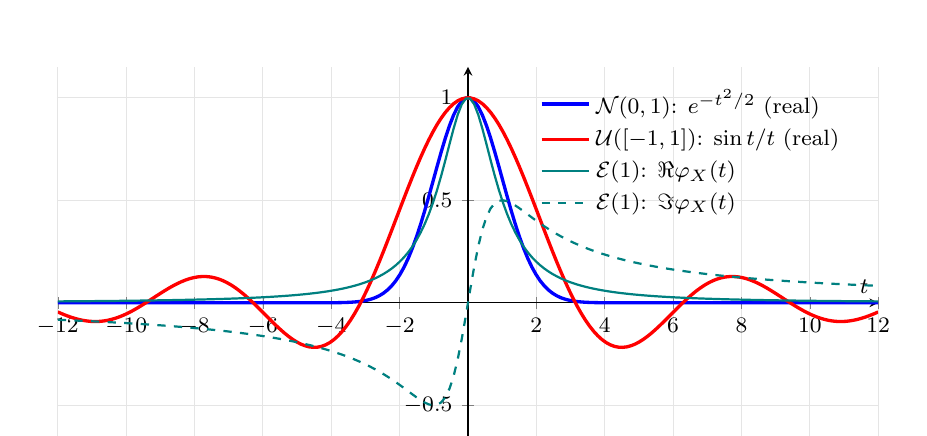
\begin{tikzpicture}
\begin{axis}[
  width=12cm, height=6.4cm, xlabel={$t$}, xmin=-12, xmax=12, ymin=-0.7, ymax=1.15,
  axis lines=middle, samples=200, domain=-12:12, grid=major, grid style={gray!20},
  legend pos=north east, legend cell align=left,
  legend style={font=\footnotesize, draw=none, fill=none},
  tick label style={font=\footnotesize}, label style={font=\footnotesize},
]
\addplot[very thick, blue]  {exp(-x^2/2)};
\addlegendentry{$\mathcal{N}(0,1)$: $e^{-t^{2}/2}$ (real)}
\addplot[very thick, red]   {sin(deg(x))/x};
\addlegendentry{$\mathcal{U}([-1,1])$: $\sin t / t$ (real)}
\addplot[thick, teal]       {1/(1+x^2)};
\addlegendentry{$\mathcal{E}(1)$: $\Re \varphi_{X}(t)$}
\addplot[thick, teal, dashed] {x/(1+x^2)};
\addlegendentry{$\mathcal{E}(1)$: $\Im \varphi_{X}(t)$}
\end{axis}
\end{tikzpicture}
\caption{Fonctions caractéristiques of three lois on a shared axis. The two
lois symétriques give real-valued curves; the exponential, which is not symétrique, needs both
a real and an imaginary part. All four curves pass through or below the level $1$, and the
two real ones take the value $1$ at $t = 0$.}
\end{figure}

\begin{figure}[ht]
\centering
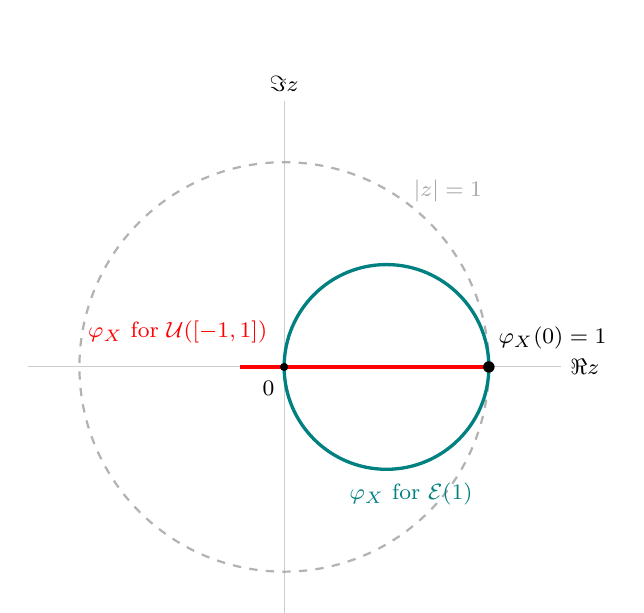
\begin{tikzpicture}[scale=2.6]
\draw[gray!40] (-1.25,0) -- (1.35,0) node[right, font=\footnotesize, black] {$\Re z$};
\draw[gray!40] (0,-1.25) -- (0,1.3) node[above, font=\footnotesize, black] {$\Im z$};
\draw[thick, gray!60, dashed] (0,0) circle (1);
\node[gray!70, font=\footnotesize] at (0.80,0.86) {$|z| = 1$};
\draw[very thick, teal] (0.5,0) circle (0.5);
\node[teal, font=\footnotesize] at (0.62,-0.62) {$\varphi_{X}$ for $\mathcal{E}(1)$};
\draw[very thick, red] (-0.2172,0) -- (1,0);
\node[red, font=\footnotesize] at (-0.52,0.17) {$\varphi_{X}$ for $\mathcal{U}([-1,1])$};
\fill (1,0) circle (0.028);
\node[font=\footnotesize, anchor=south west] at (1.0,0.04) {$\varphi_{X}(0) = 1$};
\fill (0,0) circle (0.02);
\node[font=\footnotesize, anchor=north east] at (0,-0.02) {$0$};
\end{tikzpicture}
\caption{The bound $|\varphi_{X}(t)| \leq 1 = \varphi_{X}(0)$, drawn in the
complex plane. Whatever the loi, the trajectory $t \mapsto \varphi_{X}(t)$ stays inside the
closed unit disc and touches its boundary at $t = 0$. For $\mathcal{E}(1)$ the trajectory is
exactly the circle of centre $1/2$ and radius $1/2$, tangent to the unit circle at $1$; for
the loi symétrique $\mathcal{U}([-1,1])$ it is a real segment, $\sin t / t$ ranging over
$[-0.2172\ldots,\,1]$.}
\end{figure}

\subsection{Formule d'inversion}

La \textbf{formule d'inversion} (\textit{inversion formula}) permet d'exprimer la loi d'une variable aléatoire réelle à partir de sa
fonction caractéristique. Avant d'énoncer ce résultat, on montre comment obtenir les atomes de
la loi --- by the same technique, worth seeing first because the whole proof of the formule
d'inversion is that computation with a better kernel.

\begin{prop}[Atomes de la loi]
Soit $X$ une variable aléatoire réelle. Alors,
\[
  \forall x \in \reals, \qquad \prob(X = x) = \lim_{T \to +\infty} \frac{1}{2T}\int_{-T}^{T}
  e^{-itx}\,\varphi_{X}(t)\,dt.
\]
\end{prop}

\begin{remark}
The mechanism is a Dirichlet-kernel computation followed by an exchange of limit,
espérance and integral. On fixe $x$. Pour tout $y \neq x$,
\[
  \frac{1}{2T}\int_{-T}^{T} e^{-itx}e^{ity}\,dt = \frac{1}{2T}\,\frac{e^{iT(y-x)} -
  e^{-iT(y-x)}}{i(y-x)} = \frac{\sin\!\left(T(y-x)\right)}{T(y-x)},
\]
which tends to $0$ as $T \to +\infty$; for $y = x$ the integrand is $1$ and the average is
$1$ for every $T$. En remplaçant $y$ par la variable aléatoire $X$ et en prenant l'espérance,
the limit inside is $\indic_{\{X = x\}}$. On conclut par le théorème de convergence dominée
et le théorème de Fubini, which move the limit and the espérance past the integral. Les
conditions de ces théorèmes sont bien réunies --- both are licensed by the same one-line
bound --- puisque :
\[
  \left|\frac{1}{2T}\int_{-T}^{T} e^{-itx}e^{itX}\,dt\right| \leq
  \frac{1}{2T}\int_{-T}^{T}\left|e^{-itx}e^{itX}\right|dt = 1,
\]
a constant, which is integrable because $\prob$ is a finite mesure.
\end{remark}

\begin{theorem}[Formule d'inversion]
Soit $X$ une variable aléatoire réelle de fonction de répartition $F_{X}$. Alors pour tous
\emph{points de continuité} $a, b$ de $F_{X}$, avec $a < b$,
\[
  F_{X}(b) - F_{X}(a) = \lim_{T \to +\infty} \frac{1}{2\pi}\int_{-T}^{T} \frac{e^{-ita} -
  e^{-itb}}{it}\,\varphi_{X}(t)\,dt.
\]
\end{theorem}

The hypothesis that $a$ and $b$ be continuity points of $F_{X}$ is not decoration. The proof
below produces, for arbitrary $a < b$, the quantity $\prob(a < X < b) + \tfrac{1}{2}\prob(X
= a) + \tfrac{1}{2}\prob(X = b)$, which equals $F_{X}(b) - F_{X}(a)$ as soon as neither
endpoint is an atom. The half weights at the endpoints are the signature of a Dirichlet
kernel and they are exactly what the continuity hypothesis kills.

\begin{proof}
On fixe $a < b$. Pour tout $T > 0$, soit :
\[
  I_{T} = \int_{-T}^{T} \frac{e^{-ita} - e^{-itb}}{it}\,e^{itx}\,dt,
\]
which is well defined: la fonction à intégrer, once extended by continuity, est continue sur
$[-T,T]$ --- near $t = 0$ the numerator vanishes to first order and cancels the $it$ in the
denominator.\\

\textbf{Step 1: reduce $I_{T}$ to Dirichlet integrals.} Splitting the range at $0$ and
substituting $t \mapsto -t$ on the negative half,
\[
  I_{T} = \int_{0}^{T} \frac{e^{-ita} - e^{-itb}}{it}\,e^{itx}\,dt + \int_{0}^{T}
  \frac{e^{ita} - e^{itb}}{-it}\,e^{-itx}\,dt
\]
\[
  \phantom{I_{T}} = \int_{0}^{T} \frac{e^{it(x-a)} - e^{-it(x-a)}}{it}\,dt - \int_{0}^{T}
  \frac{e^{it(x-b)} - e^{-it(x-b)}}{it}\,dt
\]
\[
  \phantom{I_{T}} = 2\left(\int_{0}^{T} \frac{\sin\!\left(t(x-a)\right)}{t}\,dt -
  \int_{0}^{T} \frac{\sin\!\left(t(x-b)\right)}{t}\,dt\right) = 2\left(\int_{0}^{T(x-a)}
  \frac{\sin u}{u}\,du - \int_{0}^{T(x-b)} \frac{\sin u}{u}\,du\right),
\]
the last equality by the changement de variable $u = t(x-a)$ in the first integral and $u =
t(x-b)$ in the second, valid with the sign conventions because $u \mapsto \sin u / u$ is
even.\\

\textbf{Step 2: take $T \to +\infty$ using the Dirichlet integral.} The classical Dirichlet
integral --- quoted here as an intégrale de Riemann impropre, chapter 3 recording its value $\pi$
over the whole line together with the warning that it is improper-Riemann and not
Lebesgue --- states
\[
  \int_{0}^{+\infty} \frac{\sin u}{u}\,du = \frac{\pi}{2}.
\]
Applying it to each of the two terms of Step 1, according to the signs of $x - a$ and $x -
b$, gives
\[
  \lim_{T \to +\infty} \frac{1}{2\pi}\int_{-T}^{T} \frac{e^{-ita} -
  e^{-itb}}{it}\,e^{itx}\,dt =
  \begin{cases} 1           & \text{if } x \in\, ]a,b[,\\[2pt]
  \tfrac{1}{2} & \text{if } x \in \{a,b\},\\[2pt] 0           & \text{otherwise.}
  \end{cases}
\]
En remplaçant $x$ par la variable aléatoire $X$ et en prenant l'espérance of this limit,
\[
  \expec\!\left(\lim_{T \to +\infty} \frac{1}{2\pi}\int_{-T}^{T} \frac{e^{-ita} -
  e^{-itb}}{it}\,e^{itX}\,dt\right) = \prob(a < X < b) + \tfrac{1}{2}\prob(X = a) +
  \tfrac{1}{2}\prob(X = b).
\]

\textbf{Step 3: exchange the limit and the espérance.} Par le théorème de convergence
dominée, the limit comes out of the espérance:
\[
  \lim_{T \to +\infty} \frac{1}{2\pi}\,\expec\!\left(\int_{-T}^{T} \frac{e^{-ita} -
  e^{-itb}}{it}\,e^{itX}\,dt\right) = \prob(a < X < b) + \tfrac{1}{2}\prob(X = a) +
  \tfrac{1}{2}\prob(X = b).
\]
Les conditions d'application du théorème sont bien satisfaites car Step 1 has already bounded
the integral, uniformly in $T$ and in $X$, by a finite constant:
\[
  \forall T \geq 0, \qquad \left|\int_{-T}^{T} \frac{e^{-ita} -
  e^{-itb}}{it}\,e^{itX}\,dt\right| \leq 4 \sup_{s \geq 0} \left|\int_{0}^{s} \frac{\sin
  u}{u}\,du\right| < \infty,
\]
the supremum being finite because $s \mapsto \int_{0}^{s}\sin u / u\,du$ is continuous with
a finite limit at $+\infty$. A constant is integrable under a mesure de probabilité, so
convergence dominée applies.\\

\textbf{Step 4: exchange the espérance and the $dt$ integral.} Le théorème de Fubini donne :
\[
  \expec\!\left(\int_{-T}^{T} \frac{e^{-ita} - e^{-itb}}{it}\,e^{itX}\,dt\right) =
  \int_{-T}^{T} \frac{e^{-ita} - e^{-itb}}{it}\,\expec\!\left(e^{itX}\right)dt =
  \int_{-T}^{T} \frac{e^{-ita} - e^{-itb}}{it}\,\varphi_{X}(t)\,dt.
\]
Fubini needs the mesure produit to be $\sigma$-finie --- it is, $\prob$ being finite and the
mesure de Lebesgue on the bounded interval $[-T,T]$ being finite too --- and needs the integrand
to be integrable for the mesure produit. À nouveau, les conditions d'application du théorème
sont bien satisfaites car, for every real $x$,
\[
  \left|\frac{e^{-ita} - e^{-itb}}{it}\,e^{itx}\right| = \left|\frac{e^{it(b-a)/2} -
  e^{-it(b-a)/2}}{t}\right| = \left|\frac{2\sin\!\left(t(b-a)/2\right)}{t}\right| \leq b -
  a,
\]
de sorte que
\[
  \expec\!\left(\left|\int_{-T}^{T} \frac{e^{-ita} -
  e^{-itb}}{it}\,e^{itX}\,dt\right|\right) \leq 2T\,(b-a) < \infty.
\]

\textbf{Step 5: conclude.} Finalement, combining Steps 3 and 4,
\[
  \lim_{T \to +\infty} \frac{1}{2\pi}\int_{-T}^{T} \frac{e^{-ita} -
  e^{-itb}}{it}\,\varphi_{X}(t)\,dt = \prob(a < X < b) + \tfrac{1}{2}\prob(X = a) +
  \tfrac{1}{2}\prob(X = b).
\]
Lorsque $a$ et $b$ sont des points de continuité de $F_{X}$, the two atoms vanish and the
right-hand side is $\prob(a < X \leq b) = F_{X}(b) - F_{X}(a)$: on obtient le résultat
annoncé.
\end{proof}

\begin{remark}
Each exchange in the proof is justified by its own explicit bound --- $4\sup_{s}
\left|\int_{0}^{s}\sin u/u\right|$ for convergence dominée, $b-a$ for Fubini --- and that is
the shape of every serious computation here: write the kernel, bound it by something
integrable that does not depend on the parameter being sent to a limit, then exchange. The
bound $\left|\sin(cs)/s\right| \leq |c|$ is used twice and is worth remembering separately.
\end{remark}

\begin{corollary}[Caractérisation de la loi]
Pour toutes variables aléatoires réelles $X, Y$, on a
\[
  \prob_{X} = \prob_{Y} \iff \varphi_{X} = \varphi_{Y}.
\]
\end{corollary}

\begin{remark}
La condition nécessaire est immédiate, par le théorème de transfert: equal lois give equal
espérances of every bounded mesurable function, in particular of $x \mapsto e^{itx}$. The
converse is the formule d'inversion plus one countability argument. Soit $A$ et $B$ les
ensembles des atomes of the two lois; ces ensembles étant au plus dénombrables, c'est
également le cas de $A \union B$, whose complement is therefore dense and unbounded below.
Pour tout $b \notin A \union B$, la formule d'inversion donne $F_{X}(b) -
F_{X}(a) = F_{Y}(b) - F_{Y}(a)$ for every $a \notin A \union B$, and letting $a \to -\infty$
en dehors de $A \union B$ yields $F_{X}(b) = F_{Y}(b)$; par ailleurs, pour tout
$b \in A \union B$, right continuity gives $F_{X}(b) = \lim_{a \downarrow b} F_{X}(a)$, the
limit again taken en dehors de $A \union B$, and the same for $Y$. On a finalement
$F_{X} = F_{Y}$, si bien que $\prob_{X} = \prob_{Y}$.
\end{remark}

La fonction caractéristique porte bien son nom, au sens où elle caractérise la loi, and this
is what every later use rests on: to identify the loi of a complicated variable aléatoire,
compute its fonction caractéristique and recognise the answer. Chapters 7 and 8 both identify
a loi that way.

\begin{corollary}[Formule d'inversion pour une loi à densité]
Soit $X$ une variable aléatoire réelle dont la fonction caractéristique est \emph{intégrable
sur $\reals$}. Alors $X$ a pour densité la fonction :
\[
  \forall x \in \reals, \qquad f_{X}(x) = \frac{1}{2\pi}\int e^{-itx}\,\varphi_{X}(t)\,dt.
\]
\end{corollary}

\begin{remark}
The integrability of $\varphi_{X}$ over the whole line is the hypothesis that makes this
work and it cannot be weakened to the boundedness the first proposition of the chapter gives
for free. It does two jobs. First it kills the atoms --- la loi n'a pas d'atome --- by the
atom formula,
\[
  \left|\frac{1}{2T}\int_{-T}^{T}e^{-itx}\varphi_{X}(t)\,dt\right| \leq
  \frac{1}{2T}\int_{-T}^{T}\left|\varphi_{X}(t)\right|dt \leq \frac{1}{2T}\int
  \left|\varphi_{X}(t)\right|dt \xrightarrow[T \to +\infty]{} 0,
\]
so $\prob(X = x) = 0$ for every $x$ and the half-weight terms of the formule d'inversion drop.
Second it licenses a Fubini and a convergence dominée in the computation
\[
  \prob(a < X < b) = \lim_{T\to+\infty}
  \frac{1}{2\pi}\int_{-T}^{T}\left(\int_{a}^{b}e^{-itx}dx\right)\varphi_{X}(t)\,dt =
  \int_{a}^{b}\left(\frac{1}{2\pi}\int e^{-itx}\varphi_{X}(t)\,dt\right)dx,
\]
which exhibits the bracketed function as a densité of $X$ on every interval, hence --- the
intervals generating $\mathcal{B}(\reals)$ --- as a densité. Note the asymmetry of the two
formulas: $\varphi_{X}$ is an integral of $e^{itx}$ against the loi, and $f_{X}$ an integral
of $e^{-itx}$ against $\varphi_{X}$, divided by $2\pi$.
\end{remark}

\begin{example}[Recovering the Cauchy densité from its fonction caractéristique]
Let $\varphi_{X}(t) = e^{-|t|}$. By the théorème de Bochner, cette fonction est la fonction
caractéristique d'une certaine variable aléatoire réelle $X$ --- it is continuous, equal to $1$
at $0$ and bounded by $1$, and it is définie positive, which is the extra hypothesis the
théorème de Bochner asks for and which is not checked here --- and it is integrable on
$\reals$, with $\int e^{-|t|}dt = 2$. The formule d'inversion pour une loi à densité therefore
applies and gives
\[
  f_{X}(x) = \frac{1}{2\pi}\int e^{-itx}e^{-|t|}\,dt =
  \frac{1}{2\pi}\left(\int_{-\infty}^{0} e^{-itx}e^{t}\,dt + \int_{0}^{+\infty}
  e^{-itx}e^{-t}\,dt\right)
\]
\[
  \phantom{f_{X}(x)} = \frac{1}{2\pi}\left(\frac{1}{1 - ix} + \frac{1}{1 + ix}\right) =
  \frac{1}{2\pi}\cdot\frac{2}{1 + x^{2}} = \frac{1}{\pi\left(1 + x^{2}\right)}.
\]
Il s'agit de la loi de Cauchy. The example is instructive twice
over: it is a loi produced from a fonction caractéristique rather than the other way round,
and it is the standard counter-example of the next subsection, having no espérance at all.
\end{example}

\subsection{Calcul de moments}

The second use of the fonction caractéristique is the one chapter 1 had for the fonction
génératrice: derivatives at a point return moments. Here the point is $0$ rather than $1^{-}$,
and the derivatives are two-sided.

\begin{definition}[Moment]
Soit $k$ un entier non nul. On appelle \textbf{moment d'ordre $k$} (\textit{moment of order
$k$}) d'une variable aléatoire réelle $X$ la valeur $\expec(X^{k})$, lorsqu'elle est bien
définie. On dit que $X$ \textbf{admet un moment d'ordre $k$} si cette valeur est finie.
\end{definition}

\begin{lemma}
Une variable aléatoire $X$ qui admet un moment d'ordre $k$ admet des moments jusqu'à l'ordre
$k$ (au moins).
\end{lemma}

\begin{remark}
One line of algebra. On a pour tout $j = 1,\dots,k$,
\[
  |X|^{j} \leq \max\!\left(|X|^{k},\,1\right) \leq |X|^{k} + 1,
\]
the first inequality because $u \mapsto u^{j}$ is below $\max(u^{k},1)$ on $\reals_{+}$ for
$j \leq k$. En appliquant l'espérance, $\expec(|X|^{j})$ is finite whenever $\expec(|X|^{k})$
is, and $\expec(1) = 1 < \infty$ because $\prob$ is a mesure de probabilité. The lemma is what
lets the moment theorem differentiate $k$ times rather than only once.
\end{remark}

\begin{theorem}[Calcul de moments]
Si la variable aléatoire $X$ \emph{admet un moment d'ordre $k$}, alors sa fonction
caractéristique $\varphi_{X}$ est $k$ fois dérivable en $0$ et
\[
  \varphi_{X}^{(k)}(0) = i^{k}\,\expec\!\left(X^{k}\right).
\]
Réciproquement, si la fonction caractéristique $\varphi_{X}$ est $k$ fois dérivable en $0$,
\emph{avec $k$ pair}, alors la variable aléatoire $X$ admet des moments jusqu'à l'ordre $k$
et ceux-ci sont donnés par la formule précédente.
\end{theorem}

Both hypotheses are load-bearing and neither may be dropped. The direct implication needs
$X$ to admit a moment d'ordre $k$ --- without it there is nothing to dominate the $k$-th
derivative of the integrand and the conclusion itself fails --- $\varphi_{X}$ need not
even be differentiable at $0$ --- as the loi de Cauchy shows below. The converse needs $k$
\emph{even} because the proof does: the sign identity
$-\varphi_{X}''(0) = \left|\varphi_{X}''(0)\right|$, and the induction step behind it, rest
on the positivity of $X^{2p}\left(1 - \cos(tX)\right)$. The caveat stated separately below ---
that $\varphi_{X}$ being of class $C^{1}$ does not make $X$ integrable --- is the same
restriction at the first order.

\begin{remark}
\textbf{The direct implication.} Pour tout $x$ réel, on a :
\[
  \frac{\partial^{k}}{\partial t^{k}}\,e^{itx} = i^{k}x^{k}e^{itx}, \qquad\text{hence}\qquad
  \left|\frac{\partial^{k}}{\partial t^{k}}\,e^{itX}\right| = |X|^{k},
\]
a dominating function that does not depend on $t$ and is integrable exactly because $X$
admet un moment d'ordre $k$. The lemma above supplies the same for every intermediate order
$j \leq k$, so \textbf{le théorème de dérivabilité sous le signe somme} of chapter 3 may
be applied $k$ times in succession --- that theorem is the dependency, and it is what the
hypothesis on the moment is there to feed. Evaluating at $t = 0$, on en déduit que :
\[
  \varphi_{X}^{(k)}(0) = \frac{\partial^{k}}{\partial
  t^{k}}\expec\!\left(e^{itX}\right)\Big|_{t=0} = i^{k}\,\expec\!\left(X^{k}\right).
\]
\end{remark}

\begin{remark}
\textbf{The converse.} A Taylor expansion at $0$ turned into an inequality by the lemme de
Fatou, run at $k = 2$ and then by induction on $p$ for $k = 2p$. Two-fold
differentiability at $0$ and the identity
$\varphi_{X}(t) + \varphi_{X}(-t) = 2\,\expec\!\left(\cos(tX)\right)$ give
\[
  \lim_{t \to 0} \frac{2}{t^{2}}\,\expec\!\left(1 - \cos(tX)\right) = -\varphi_{X}''(0) =
  \left|\varphi_{X}''(0)\right|,
\]
la dernière égalité venant du fait que le terme de gauche est positif, $1 - \cos \geq 0$ ---
which is exactly where the parity of $k$ enters. Along any $t_{n} \to 0$ the integrand tends
to $X^{2}$, so, par le lemme de Fatou, $\expec(X^{2})$ is bounded by
$\left|\varphi_{X}''(0)\right| < \infty$. The
induction step repeats this with $\varphi_{X}^{(2p)}$ in place of $\varphi_{X}$, using the
induction hypothesis $\varphi_{X}^{(2p)}(0) = (-1)^{p}\expec(X^{2p})$ and differentiating
the same cosine identity $2p$ times under the integral sign, to bound
$\expec(X^{2p+2})$ by $\left|\varphi_{X}^{(2p+2)}(0)\right| < \infty$.
\end{remark}

\begin{remark}
A caveat that is easy to lose: il n'est \textbf{pas} suffisant que la fonction
caractéristique $\varphi_{X}$ soit de classe $C^{1}$ pour que la variable aléatoire $X$ soit
intégrable. Une condition suffisante est que $\varphi_{X}$ soit de classe $C^{2}$. This is the
same parity phenomenon as in the theorem, stated for the weakest case: one derivative buys
nothing, two buy a first and a second moment.
\end{remark}

In practice the theorem is almost never applied by differentiating $k$ times. It is applied
by expanding $\varphi_{X}$ in a Taylor series at $0$ and reading the coefficients: once
$\varphi_{X}$ is known to be $k$ times differentiable at $0$, the theorem fixes its Taylor
coefficients as the $i^{j}\expec(X^{j})/j!$, so matching any expansion against
$\sum_{j \leq k} i^{j}\expec(X^{j})\,t^{j}/j! + o(t^{k})$ reads the moments off. The
expansion alone is weaker than the differentiability the theorem asks for, so it is a way of
applying the theorem and not a restatement of it. Three examples show the pattern, and one
shows the failure.

\begin{example}[Moments de la loi exponentielle]
For $X \sim \mathcal{E}(\lambda)$ the fonction caractéristique $\varphi_{X}(t) =
\lambda/(\lambda - it)$ expands as a geometric series in $it/\lambda$:
\[
  \varphi_{X}(t) = \frac{1}{1 - it/\lambda} = 1 + \frac{it}{\lambda} +
  \left(\frac{it}{\lambda}\right)^{2} + o(t^{2}) = 1 + \frac{it}{\lambda} -
  \frac{t^{2}}{\lambda^{2}} + o(t^{2}).
\]
Matching against $1 + i\expec(X)t - \expec(X^{2})t^{2}/2 + o(t^{2})$ gives
\[
  \expec(X) = \frac{1}{\lambda}, \qquad \expec\!\left(X^{2}\right) = \frac{2}{\lambda^{2}},
  \qquad \Var(X) = \frac{2}{\lambda^{2}} - \frac{1}{\lambda^{2}} = \frac{1}{\lambda^{2}}.
\]
\end{example}

\begin{example}[{Moments de la loi uniforme sur $[0,1]$}]
For $X \sim \mathcal{U}([0,1])$, $\varphi_{X}(t) = \left(e^{it}-1\right)/(it)$ for $t \neq
0$. Comme $e^{it} = 1 + it - t^{2}/2 - it^{3}/6 + o(t^{3})$, on obtient, dividing by $it$ :
\[
  \varphi_{X}(t) = 1 + \frac{it}{2} - \frac{t^{2}}{6} + o(t^{2}),
\]
on en déduit
\[
  \expec(X) = \frac{1}{2}, \qquad \expec\!\left(X^{2}\right) = \frac{1}{3}, \qquad \Var(X) =
  \frac{1}{3} - \frac{1}{4} = \frac{1}{12}.
\]
\end{example}

\begin{example}[Moments de la loi Gamma]
For $X \sim \Gamma(a,\lambda)$, $\varphi_{X}(t) = (1 - it/\lambda)^{-a}$, and the binomial
series $(1-u)^{-a} = 1 + au + a(a+1)u^{2}/2 + o(u^{2})$ with $u = it/\lambda$ gives
\[
  \varphi_{X}(t) = 1 + \frac{ia\,t}{\lambda} - \frac{a(a+1)}{2}\,\frac{t^{2}}{\lambda^{2}} +
  o(t^{2}),
\]
so that
\[
  \expec(X) = \frac{a}{\lambda}, \qquad \expec\!\left(X^{2}\right) =
  \frac{a(a+1)}{\lambda^{2}}, \qquad \Var(X) = \frac{a(a+1) - a^{2}}{\lambda^{2}} =
  \frac{a}{\lambda^{2}}.
\]
Setting $a = 1$ recovers the exponential line above, as a check.
\end{example}

\begin{example}[Les quatre premiers moments de la loi normale centrée réduite]
For $X \sim \mathcal{N}(0,1)$, $\varphi_{X}(t) = e^{-t^{2}/2}$, and expanding the
exponential to two terms,
\[
  \varphi_{X}(t) = 1 - \frac{t^{2}}{2} + \frac{t^{4}}{8} + o\!\left(t^{4}\right).
\]
The odd powers are absent, which is the symmetry of the loi reappearing. Matching
coefficients against $\sum_{j \leq 4} i^{j}\expec(X^{j})t^{j}/j!$ gives
\[
  \expec(X) = 0, \qquad \expec\!\left(X^{2}\right) = 1, \qquad \expec\!\left(X^{3}\right) =
  0, \qquad \expec\!\left(X^{4}\right) = 3.
\]
The fourth moment being $3$ rather than $1$ is the value worth memorising, and it is read
straight off the $t^{4}$ coefficient of $e^{-t^{2}/2}$.
\end{example}

\begin{example}[A loi whose fonction caractéristique is not differentiable at zero]
La loi de Cauchy n'a pas d'espérance: $\int |x|/(\pi(1+x^{2}))\,dx$ diverges logarithmically.
Its fonction caractéristique is $\varphi_{X}(t) = e^{-|t|}$, which is continuous everywhere,
of modulus at most $1$, equal to $1$ at $0$ --- and cette fonction n'est \emph{pas} dérivable
en $0$, the left and right derivatives being $+1$ and $-1$. The theorem's direct implication
is therefore consistent: a loi with no moment d'ordre $1$ may not have a differentiable
fonction caractéristique at $0$. This is the example to reach for whenever the hypothesis
``$X$ admet un moment d'ordre $k$'' looks removable.
\end{example}

\subsection{Somme de variables aléatoires indépendantes}

The third use --- and the one chapter 8 runs on --- is that the fonction caractéristique converts
the convolution of lois into an ordinary product of functions.

\begin{prop}
Soit $X$ et $Y$ deux variables aléatoires réelles indépendantes. La fonction caractéristique
de leur somme est donnée par :
\[
  \forall t \in \reals, \qquad \varphi_{X+Y}(t) = \varphi_{X}(t)\,\varphi_{Y}(t).
\]
\end{prop}

\begin{proof}
Fix $t \in \reals$. Since $X \indep Y$, the variables aléatoires $e^{itX}$ and $e^{itY}$ are
independent as well, being mesurable functions of $X$ and of $Y$ respectively; both are
bounded, hence integrable, so the product rule for espérances of independent integrable
variables applies:
\[
  \varphi_{X+Y}(t) = \expec\!\left(e^{it(X+Y)}\right) =
  \expec\!\left(e^{itX}\,e^{itY}\right) =
  \expec\!\left(e^{itX}\right)\expec\!\left(e^{itY}\right) = \varphi_{X}(t)\,\varphi_{Y}(t).
\]
\end{proof}

\begin{remark}
One line, and it is worth noticing what does \emph{not} appear in it. There is no
integrability hypothesis on $X$ or $Y$, because $e^{itX}$ and $e^{itY}$ are bounded whatever
the lois; there is no hypothesis of a densité, so the result covers discrete and continuous
lois at once; and there is no convolution integral to compute. Combined with the corollary
that the fonction caractéristique determines the loi, the proposition is a complete method
for finding the loi of a sum of independent variables: multiply, then recognise. By
induction it extends immediately to $n$ independent summands, and for $n$ i.i.d.\ summands
it reads $\varphi_{S_{n}} = \varphi_{X_{1}}^{\,n}$ --- which is the identity the théorème
central limite is proved from in chapter 8.
\end{remark}

\begin{figure}[ht]
\centering
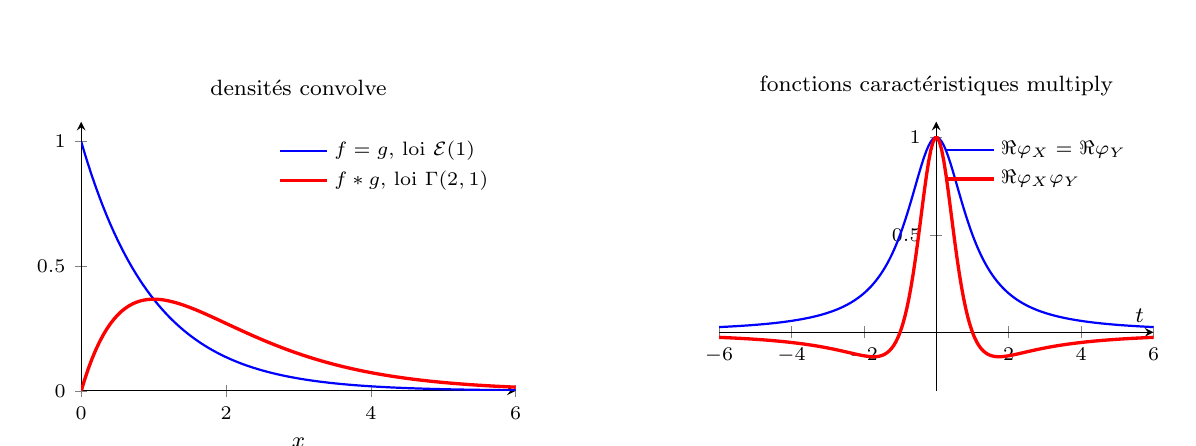
\begin{tikzpicture}
\begin{axis}[
  name=densities, width=7.1cm, height=5.0cm, xlabel={$x$},
  title={\footnotesize densités convolve}, title style={font=\footnotesize},
  xmin=0, xmax=6, ymin=0, ymax=1.08, axis lines=left, samples=120, domain=0:6,
  legend pos=north east, legend cell align=left,
  legend style={font=\scriptsize, draw=none, fill=none},
  tick label style={font=\scriptsize}, label style={font=\footnotesize},
]
\addplot[thick, blue] {exp(-x)};
\addlegendentry{$f = g$, loi $\mathcal{E}(1)$}
\addplot[very thick, red] {x*exp(-x)};
\addlegendentry{$f * g$, loi $\Gamma(2,1)$}
\end{axis}
\begin{axis}[
  at={(8.1cm,0cm)}, anchor=south west, width=7.1cm, height=5.0cm, xlabel={$t$},
  title={\footnotesize fonctions caractéristiques multiply}, title style={font=\footnotesize},
  xmin=-6, xmax=6, ymin=-0.3, ymax=1.08, axis lines=middle, samples=200, domain=-6:6,
  legend pos=north east, legend cell align=left,
  legend style={font=\scriptsize, draw=none, fill=none},
  tick label style={font=\scriptsize}, label style={font=\footnotesize},
]
\addplot[thick, blue] {1/(1+x^2)};
\addlegendentry{$\Re \varphi_{X} = \Re \varphi_{Y}$}
\addplot[very thick, red] {(1-x^2)/((1+x^2)^2)};
\addlegendentry{$\Re \varphi_{X}\varphi_{Y}$}
\end{axis}
\end{tikzpicture}
\caption{The product rule, drawn. On the left, two $\mathcal{E}(1)$ densités
and their convolution, the $\Gamma(2,1)$ densité $x e^{-x}$; on the right, the real parts of
the corresponding fonctions caractéristiques, the product $\left(1/(1-it)\right)^{2}$ having
real part $(1-t^{2})/(1+t^{2})^{2}$. The convolution on the left costs an integral; the
product on the right costs a multiplication.}
\end{figure}

\begin{example}[A normal variable with general parameters]
Soit $Z \sim \mathcal{N}(0,1)$. La variable aléatoire $X = \sigma Z + \mu$ suit une loi normale
$\mathcal{N}(\mu,\sigma^{2})$. An affine changement de variable inside the espérance gives
\[
  \forall t \in \reals, \qquad \varphi_{X}(t) = \expec\!\left(e^{it(\sigma Z + \mu)}\right)
  = e^{i\mu t}\,\varphi_{Z}(\sigma t) = e^{i\mu t}\,e^{-\sigma^{2}t^{2}/2}.
\]
The two operations used --- $\varphi_{aX+b}(t) = e^{ibt}\varphi_{X}(at)$ --- are worth
isolating, since they are needed again in chapter 8 to normalise a sum.
\end{example}

\begin{example}[The sum of two independent normal variables is normal]
Let $X \sim \mathcal{N}(\mu_{1},\sigma_{1}^{2})$ and $Y \sim
\mathcal{N}(\mu_{2},\sigma_{2}^{2})$ be independent. Multiplying the fonctions
caractéristiques of the previous example,
\[
  \varphi_{X+Y}(t) = e^{i\mu_{1}t}e^{-\sigma_{1}^{2}t^{2}/2}\,
  e^{i\mu_{2}t}e^{-\sigma_{2}^{2}t^{2}/2} = e^{i(\mu_{1}+\mu_{2})t}\,
  e^{-\left(\sigma_{1}^{2}+\sigma_{2}^{2}\right)t^{2}/2},
\]
which is the fonction caractéristique of
$\mathcal{N}(\mu_{1}+\mu_{2},\,\sigma_{1}^{2}+\sigma_{2}^{2})$. Since the fonction
caractéristique determines the loi, the sum follows that loi: la somme de deux variables
aléatoires indépendantes suivant des lois normales suit une loi normale, d'espérance la somme
des espérances et de variance la somme des variances. The indépendance hypothesis
is essential --- without it only the means add.
\end{example}

\begin{example}[A sum of independent exponential variables is a gamma variable]
Soit $X_{1},\dots,X_{n}$ des variables aléatoires i.i.d.\ de loi $\mathcal{E}(\lambda)$ et
$S = X_{1} + \dots + X_{n}$ leur somme. The product rule and the exponential computation give
\[
  \varphi_{S}(t) = \varphi_{X_{1}}(t)\cdots\varphi_{X_{n}}(t) =
  \left(\varphi_{X_{1}}(t)\right)^{n} = \left(\frac{\lambda}{\lambda - it}\right)^{n},
\]
which is la fonction caractéristique d'une loi $\Gamma(n,\lambda)$. Hence $S \sim
\Gamma(n,\lambda)$. Computing the same convolution directly would mean $n-1$ nested
integrals.
\end{example}

\begin{example}[The gamma family is stable in its first parameter]
Soit $X \sim \Gamma(a,\lambda)$ et $Y \sim \Gamma(b,\lambda)$ indépendantes, with the
\emph{same} second parameter $\lambda$. Then
\[
  \forall t \in \reals, \qquad \varphi_{X+Y}(t) = \left(\frac{\lambda}{\lambda -
  it}\right)^{a} \left(\frac{\lambda}{\lambda - it}\right)^{b} =
  \left(\frac{\lambda}{\lambda - it}\right)^{a+b},
\]
so $X + Y \sim \Gamma(a+b,\lambda)$. The equality of the two $\lambda$'s is what makes the
exponents add; with different rate parameters the product is not of gamma form and the sum
is not a gamma variable.
\end{example}

\begin{example}[The loi du $\chi^{2}$ as a loi Gamma]
For $Z \sim \mathcal{N}(0,1)$, combining the two exponents and rescaling the Gaussian
integral --- legitimate for a complex parameter of positive real part --- gives
\[
  \varphi_{Z^{2}}(t) = \expec\!\left(e^{itZ^{2}}\right) = \int
  e^{itz^{2}}\frac{1}{\sqrt{2\pi}}e^{-z^{2}/2}\,dz = \int e^{-\frac{1}{2}(1 -
  2it)z^{2}}\frac{1}{\sqrt{2\pi}}\,dz = \frac{1}{\sqrt{1 - 2it}},
\]
which is $\left(\tfrac{1}{2}/(\tfrac{1}{2} - it)\right)^{1/2}$, la fonction caractéristique
d'une loi $\Gamma(\tfrac{1}{2},\tfrac{1}{2})$. By definition, la \textbf{loi du $\chi^{2}$ à
$n$ degrés de liberté} (\textit{chi-squared distribution with $n$ degrees of freedom}) est une
loi Gamma $\Gamma(\tfrac{n}{2},\tfrac{1}{2})$, so the previous example gives at once that la
somme des carrés de $n$ variables aléatoires normales centrées réduites indépendantes suit une
loi du $\chi^{2}$ à $n$ degrés de liberté, and that la somme de deux variables indépendantes de
lois du $\chi^{2}$ à $n$ et $m$ degrés de liberté follows a loi du $\chi^{2}$ à $n + m$
degrés de liberté.
\end{example}

\begin{example}[A geometric number of exponential summands]
Soit $X_{1}, X_{2}, \dots$ une suite de variables aléatoires i.i.d.\ de loi $\mathcal{E}(\lambda)$,
et $N$ une variable aléatoire de loi géométrique $\mathcal{G}(p)$ de paramètre $p \in\, ]0,1[$,
indépendante de cette suite. On note $S = \sum_{i=1}^{N} X_{i}$, a sum with a \emph{random}
number of terms. Conditioning on $N$ and using the
previous computation for a fixed number of summands,
\[
  \varphi_{S}(t) = \sum_{n \geq 1} \prob(N = n)\, \expec\!\left(e^{itS} \mid N = n\right) =
  \sum_{n \geq 1} (1-p)^{n-1}p\left(\frac{\lambda}{\lambda - it}\right)^{n} =
  \frac{p\lambda}{p\lambda - it},
\]
the last step being the geometric sum $\sum_{n \geq 1}(1-p)^{n-1}p\,z^{n} = pz/(1-(1-p)z)$
with $z = \lambda/(\lambda - it)$. So $S \sim \mathcal{E}(p\lambda)$: a geometric number of
independent exponential waiting times is again an exponential waiting time, with the rate
thinned by $p$. The conditioning step is the discrete espérance conditionnelle of chapter 1,
and the interchange of the sum and the espérance is convergence dominée, the partial
sums being bounded by $1$.
\end{example}

\begin{example}[The loi de Cauchy is stable under averaging]
Soit $X_{1},\dots,X_{n}$ des variables aléatoires i.i.d.\ suivant la loi de Cauchy, so
$\varphi_{X_{1}}(t) = e^{-|t|}$. The fonction caractéristique of the arithmetic mean is
\[
  \varphi_{\frac{1}{n}(X_{1}+\dots+X_{n})}(t) =
  \varphi_{X_{1}+\dots+X_{n}}\!\left(\frac{t}{n}\right) =
  \left(\varphi_{X_{1}}\!\left(\frac{t}{n}\right)\right)^{n} = \left(e^{-|t|/n}\right)^{n} =
  e^{-|t|},
\]
so la moyenne arithmétique of $n$ i.i.d.\ Cauchy variables suit une loi de Cauchy --- the same
one, whatever $n$.
Averaging buys nothing, and neither does averaging in the other sense: the inverse of a
Cauchy variable is again a Cauchy variable, so the $1/X_{i}$ are i.i.d.\ with the loi de
Cauchy, their arithmetic mean is Cauchy by the computation just made, and la moyenne
harmonique $n/(1/X_{1}+\dots+1/X_{n})$, being the inverse of that arithmetic mean, suit
également une loi de Cauchy. This
is the standard illustration that the loi forte des grands nombres and
the théorème central limite of chapter 8 genuinely need their moment hypotheses, which the
loi de Cauchy fails at the first order.
\end{example}

\begin{remark}[The parallel with the fonction génératrice of chapter 1]
The two transforms of the course have the same two uses and differ in one respect only.
\begin{itemize}
  \item \textbf{Moments by differentiation.} $G_{X}$ gives factorial moments
    from left derivatives at $1$, when those are finite, and $\varphi_{X}$ gives ordinary
    moments from two-sided derivatives at $0$, when the moment exists:
    \[
      \expec\!\left(X(X-1)\cdots(X-k+1)\right) = G_{X}^{(k)}\!\left(1^{-}\right), \qquad
      \varphi_{X}^{(k)}(0) = i^{k}\,\expec\!\left(X^{k}\right).
    \]
  \item \textbf{Products for sums of independents.} $G_{X+Y} = G_{X}G_{Y}$ and
    $\varphi_{X+Y} = \varphi_{X}\varphi_{Y}$, proved by exactly the same line: the
    exponential turns a sum into a product and indépendance splits the espérance.
  \item \textbf{The difference.} $G_{X}(t) = \expec(t^{X})$ requires $X$ to
    take values in $\mathbb{N}$ and requires $|t| \leq 1$ for the series to converge, and
    even then its derivative at $1$ may be infinite. $\varphi_{X}$ requires nothing at all:
    it is defined for every real variable aléatoire and every real $t$, because
    $\left|e^{itX}\right| = 1$. That is the whole of the advantage, and it is why the
    fonction caractéristique and not the fonction génératrice is the tool of chapters 7 and 8.
\end{itemize}
Both transforms characterise the loi --- $G_{X}$ through $\prob(X = k) = G_{X}^{(k)}(0)/k!$,
$\varphi_{X}$ through the formule d'inversion --- so the choice between them is a matter of
which is easier to compute, and for an $\mathbb{N}$-valued variable that is often $G_{X}$.
\end{remark}

\subsection{Cas des vecteurs aléatoires}

Les résultats précédents se généralisent à des vecteurs aléatoires réels. The scalar results
are deliberately restated below rather than generalised in place, in compressed form: the
statements come first and the remark that follows says which of them are word-for-word
transpositions and which are genuinely different.

\begin{definition}[Fonction caractéristique d'un vecteur aléatoire]
La \textbf{fonction caractéristique} d'un vecteur aléatoire réel $X$ de dimension $n$ est la
fonction $\varphi_{X} \colon \reals^{n} \to \mathbb{C}$ définie par :
\[
  \forall t \in \reals^{n}, \qquad \varphi_{X}(t) =
  \expec\!\left(e^{i\,t^{T}X}\right),
\]
where $t^{T}X = t_{1}X_{1} + \dots + t_{n}X_{n}$.
\end{definition}

As in dimension $1$, la fonction caractéristique est continue, telle que $\varphi_{X}(0) =
1$ et
\[
  \forall t \in \reals^{n}, \qquad \left|\varphi_{X}(t)\right| \leq 1,
\]
for the same three reasons: continuité sous le signe somme with the constant $1$ as
dominating function, the value of the integrand at $t = 0$, and the modulus inequality
applied to a variable of modulus $1$.

\begin{theorem}[Formule d'inversion pour un vecteur aléatoire]
Soit $X$ un vecteur aléatoire réel de fonction de répartition $F_{X}$. Alors pour tous points
de continuité $a, b$ de $F_{X}$, avec $a < b$ \emph{composante par composante},
\[
  F_{X}(b) - F_{X}(a) = \lim_{T_{1} \to +\infty}\ \dots \lim_{T_{n} \to +\infty}
  \frac{1}{(2\pi)^{n}}\int_{-T_{1}}^{T_{1}}\!\!\dots\int_{-T_{n}}^{T_{n}}
  \prod_{j=1}^{n}\frac{e^{-it_{j}a_{j}} - e^{-it_{j}b_{j}}}{it_{j}}\, \varphi_{X}(t)\,dt.
\]
\end{theorem}

\begin{corollary}[Caractérisation de la loi]
Pour tous vecteurs aléatoires réels $X, Y$, on a
\[
  \prob_{X} = \prob_{Y} \iff \varphi_{X} = \varphi_{Y}.
\]
\end{corollary}

\begin{corollary}[Formule d'inversion pour une loi à densité]
Soit $X$ un vecteur aléatoire réel dont la fonction caractéristique est \emph{intégrable sur
$\reals^{n}$}. Alors $X$ a pour densité la fonction :
\[
  \forall x \in \reals^{n}, \qquad f_{X}(x) = \frac{1}{(2\pi)^{n}}\int
  e^{-i\,t^{T}x}\,\varphi_{X}(t)\,dt.
\]
\end{corollary}

\begin{definition}[Moment d'un vecteur aléatoire]
Soit $k$ un entier non nul. On appelle \textbf{moment d'ordre $k$} d'un vecteur aléatoire
réel $X$ le \emph{vecteur} $\expec(X^{k})$, lorsqu'il est bien défini. On dit que $X$ admet
un moment d'ordre $k$ si ce vecteur est fini.
\end{definition}

\begin{lemma}
Soit $X$ un vecteur aléatoire réel qui admet un moment d'ordre $k$. Alors pour tous entiers
naturels $j_{1},\dots,j_{n}$ \emph{de somme inférieure ou égale à $k$},
\[
  \expec\!\left(\left|X_{1}^{j_{1}} \dots X_{n}^{j_{n}}\right|\right) < \infty.
\]
\end{lemma}

\begin{remark}
The same algebraic line as in dimension $1$, with a maximum over the components in place of
a maximum over the orders:
\[
  \left|X_{1}^{j_{1}} \dots X_{n}^{j_{n}}\right| \leq
  \max\!\left(|X_{1}|^{k},\dots,|X_{n}|^{k},\,1\right) \leq |X_{1}|^{k} + \dots +
  |X_{n}|^{k} + 1,
\]
and en appliquant l'espérance, on obtient le résultat annoncé, each term on the right being
finite by hypothesis. What the lemma controls is a \emph{mixed} moment, which has no
counterpart in dimension $1$.
\end{remark}

\begin{theorem}[Calcul de moments d'un vecteur aléatoire]
Si le vecteur aléatoire $X$ admet un moment d'ordre $k$, alors sa fonction caractéristique
$\varphi_{X}$ est $k$ fois dérivable en $0$ et pour tous entiers naturels
$j_{1},\dots,j_{n}$ \emph{de somme égale à $k$},
\[
  \frac{\partial^{\,j_{1}} \dots \partial^{\,j_{n}}} {\partial t_{1}^{\,j_{1}} \dots
  \partial t_{n}^{\,j_{n}}}\, \varphi_{X}(0) = i^{k}\,\expec\!\left(X_{1}^{j_{1}} \dots
  X_{n}^{j_{n}}\right).
\]
Réciproquement, si la fonction caractéristique $\varphi_{X}$ est $k$ fois dérivable en $0$,
\emph{avec $k$ pair}, alors les variables aléatoires $X_{1}^{j_{1}} \dots X_{n}^{j_{n}}$ sont
d'espérances finies, données par la formule précédente, pour tous entiers naturels
$j_{1},\dots,j_{n}$ \emph{de somme inférieure ou égale à $k$}.
\end{theorem}

\begin{remark}
La première partie du théorème se prouve exactly as in dimension $1$, differentiating under
the integral sign, with the vector lemma above supplying the dominating function
$\left|X_{1}^{j_{1}}\dots X_{n}^{j_{n}}\right|$ in place of $|X|^{k}$. The converse reduces
to the scalar theorem by a projection: pour tout $j = 1,\dots,n$, la fonction caractéristique
de la variable aléatoire $X_{j}$ est donnée par $\varphi_{X_{j}}(t) = \varphi_{X}(t e_{j})$
pour tout $t \in \reals$, où $e_{j}$ désigne le vecteur unitaire sur la composante $j$. Cette
fonction caractéristique étant $k$ fois dérivable en $0$, avec $k$ pair, the scalar theorem gives
$X_{j}$ a moment d'ordre $k$; le vecteur aléatoire $X$ admet donc un moment d'ordre $k$, and
the direct implication finishes.
\end{remark}

\begin{remark}[Which of these are verbatim transpositions, and which are not]
Worth separating, because reading the six statements as a block hides the two that carry new
content.
\begin{itemize}
  \item \textbf{Verbatim transpositions}, with $t^{T}x$ in place of
    $tx$ and $\reals^{n}$ in place of $\reals$: the definition of $\varphi_{X}$, the
    continuity and the bounds $\varphi_{X}(0) = 1$ and $\left|\varphi_{X}\right| \leq 1$,
    and the corollary that the fonction caractéristique characterises the loi. Nothing in
    their proofs changes.
  \item \textbf{Transpositions that change shape.} The formule d'inversion
    becomes an \emph{iterated} limit, one $T_{j}$ per coordinate, over a product of $n$
    scalar kernels and with $(2\pi)^{n}$ in the denominator; its hypothesis is that $a < b$
    hold componentwise, which is strictly stronger than $a < b$ for vectors read any other
    way. The formule d'inversion pour une loi à densité keeps the same shape but with
    $(2\pi)^{n}$ and the scalar product in the exponent, and its hypothesis is integrability
    over the whole of $\reals^{n}$.
  \item \textbf{Genuinely different statements.} The lemma is about
    \emph{mixed} moments $\expec\left(\left|X_{1}^{j_{1}}\dots X_{n}^{j_{n}}\right|\right)$
    with $j_{1}+\dots+j_{n} \leq k$, where the scalar lemma was about lower-order moments
    $\expec(|X|^{j})$ with $j \leq k$; and the moment theorem returns \emph{mixed partial}
    derivatives, one formula for each multi-index of total order $k$, where the scalar
    theorem returned one number per order. The converse also changes method, going through
    the projections $\varphi_{X_{j}}(t) = \varphi_{X}(te_{j})$ rather than repeating the
    Fatou argument in $n$ dimensions.
\end{itemize}
The product rule for sums of independent \emph{vectors} holds too, by the same one-line
proof, and is used in chapter 7 to add independent vecteurs gaussiens.
\end{remark}

\subsection{Caractérisation de l'indépendance}

The last result of the chapter is the one chapter 7 is built on. It says that indépendance
of the components of a vecteur aléatoire is not merely implied by a factorisation of the joint
fonction caractéristique --- it is equivalent to it.

\begin{prop}[Caractérisation de l'indépendance]
Soit $X$ un vecteur aléatoire de dimension $n$. Les composantes $X_{1},\dots,X_{n}$ du vecteur
$X$ sont indépendantes si et seulement si
\[
  \forall t \in \reals^{n}, \qquad \varphi_{X}(t) = \varphi_{X_{1}}(t_{1}) \dots
  \varphi_{X_{n}}(t_{n}).
\]
\end{prop}

\begin{remark}
\textbf{La condition nécessaire} est immédiate: if the components are independent then so are
the bounded variables $e^{it_{1}X_{1}},\dots,e^{it_{n}X_{n}}$, and the espérance of their
product splits,
\[
  \varphi_{X}(t) = \expec\!\left(e^{i\,t^{T}X}\right) =
  \expec\!\left(e^{it_{1}X_{1}}\right)\dots\expec\!\left(e^{it_{n}X_{n}}\right) =
  \varphi_{X_{1}}(t_{1})\dots\varphi_{X_{n}}(t_{n}).
\]
\textbf{The sufficient condition} is the interesting direction and it is a one-trick
argument: build a comparison vector and appeal to uniqueness. On considère un vecteur $Y$
dont les composantes sont indépendantes, de mêmes lois marginales que le vecteur $X$ --- such a
$Y$ exists, on a product space, by the mesure produit construction of chapter 3. By the
direction just proved,
\[
  \forall t \in \reals^{n}, \qquad \varphi_{Y}(t) =
  \varphi_{Y_{1}}(t_{1})\dots\varphi_{Y_{n}}(t_{n}) =
  \varphi_{X_{1}}(t_{1})\dots\varphi_{X_{n}}(t_{n}) = \varphi_{X}(t),
\]
the middle equality because $Y_{j}$ and $X_{j}$ have the same loi and hence the same
fonction caractéristique, and the last by hypothesis. The vector corollary that the
fonction caractéristique characterises the loi then gives $\prob_{X} = \prob_{Y}$;
indépendance of the components being a property of the loi jointe alone, the components of
$X$ are independent.
\end{remark}

\begin{remark}
The criterion is a genuine strengthening of what the definition of indépendance gives.
Verifying indépendance from the definition means checking $\prob(X_{1} \in A_{1}, \dots,
X_{n} \in A_{n}) = \prod_{j}\prob(X_{j} \in A_{j})$ for all boréliens $A_{1},\dots,A_{n}$ ---
an uncountable family of conditions on sets. The criterion replaces it by one functional
identity between two explicit functions on $\reals^{n}$, both of which are usually written
down in closed form. Chapter 7 uses it in exactly that way: the fonction caractéristique of a
vecteur gaussien of matrice de covariance $\Gamma$ is $\varphi_{X}(t) =
\exp\!\left(i\,t^{T}\mu - \tfrac{1}{2}t^{T}\Gamma t\right)$, and that
expression factorises into a product of $n$ scalar Gaussian fonctions caractéristiques exactly
when the quadratic form $t^{T}\Gamma t$ has no cross terms, that is, exactly when
$\Gamma$ is diagonal. So for a vecteur gaussien --- and only because the criterion is an
equivalence --- décorrélées components are independent components.
\end{remark}

\begin{conclusion}
The fonction caractéristique $\varphi_{X}(t) = \expec\left(e^{itX}\right)$ exists for every
real variable aléatoire, with no hypothesis, because $\left|e^{itX}\right| = 1$; it is
continuous, equals $1$ at $0$ and is bounded by $1$ in modulus. The formule d'inversion
recovers $F_{X}$ from $\varphi_{X}$ at every pair of continuity points, and therefore
$\varphi_{X}$ determines the loi; when $\varphi_{X}$ is integrable over $\reals$ the same
formula produces a densité. The $k$-th derivative at $0$ returns $i^{k}\expec(X^{k})$ when
the moment d'ordre $k$ exists, and conversely a derivative of even order $k$ at $0$ forces
the moments up to order $k$ to exist. For independent variables $\varphi_{X+Y} =
\varphi_{X}\varphi_{Y}$, which turns convolutions into products. All of this transposes to
vecteurs aléatoires, the formule d'inversion becoming an iterated limit and the moment theorem
returning mixed partial derivatives, and the transposition yields the criterion the next
chapter needs: the components of a vecteur aléatoire are independent exactly when the joint
fonction caractéristique factorises into the product of the marginal ones.
\end{conclusion}

\section{Vecteurs gaussiens}

Vecteurs gaussiens are the one family of multivariate lois this course
handles in closed form, and two facts make that possible. The loi of a vecteur
gaussien is determined by two objects only, a mean vector and a matrice de
covariance, so every question about it reduces to linear algebra; and the family is
stable under every affine map, so the answer to such a question is again a
vecteur gaussien. What follows is the consequence of those two facts, together
with one counter-example showing that the definition which makes them true
cannot be weakened to the one a reader expects. Les vecteurs gaussiens
apparaissent également dans le théorème central limite, présenté au chapitre
suivant, as its limit.

\subsection{Rappels sur la loi normale}

Nous commençons par revoir les principales propriétés de la loi normale --- the
one-dimensional case, which chapter 4 introduced as a loi with a densité and
which this chapter needs in the sharper form of its fonction caractéristique.

\begin{definition}[Loi normale]
Une variable aléatoire réelle $X$ suit une loi normale d'espérance $\mu$ et de
variance $\sigma^{2}$, ce que l'on note $X \sim \mathcal{N}(\mu,\sigma^{2})$, si
elle a pour densité :
\[
  \forall x \in \reals, \qquad
  f_{X}(x) = \frac{1}{\sqrt{2\pi}\,\sigma}\,
             e^{-\frac{(x-\mu)^{2}}{2\sigma^{2}}} .
\]
Le paramètre $\sigma > 0$ est l'\textbf{écart type}
(\textit{standard deviation}) de $X$. La loi normale est également appelée
\textbf{loi gaussienne} (\textit{Gaussian distribution}), and the two names are
used interchangeably throughout.
\end{definition}

\begin{notation}
Par convention, on inclut dans les lois normales les mesures de Dirac. Ainsi une
mesure de Dirac en $\mu$ sera vue comme une loi normale d'espérance $\mu$ et
d'écart type $\sigma = 0$. Cette loi n'a évidemment pas de densité par rapport
à la mesure de Lebesgue, and the definition above does not cover
it --- it is a convention, not a theorem. It is kept because without it the
statements later in this chapter would each need a separate clause for the
dégénéré case: an affine image of a vecteur gaussien can be constant, a vecteur
gaussien with a singular matrice de covariance has components that are constant
along some direction, and in both cases the convention lets the result be stated
without an exception.
\end{notation}

Si $Z$ est une variable aléatoire suivant une loi normale centrée réduite, soit
$Z \sim \mathcal{N}(0,1)$, alors la variable aléatoire
\[
  X = \sigma Z + \mu
\]
suit une loi normale d'espérance $\mu$ et de variance $\sigma^{2}$. This
is the changement de variable computation of chapter 4, and it is the form in
which the loi normale is used here: everything Gaussian in this chapter is
built as an affine image of something centré réduit.

\begin{prop}[Fonction caractéristique de la loi normale]
La fonction caractéristique d'une variable aléatoire réelle $X$ suivant une loi
normale d'espérance $\mu$ et de variance $\sigma^{2}$ est donnée par :
\[
  \forall t \in \reals, \qquad
  \varphi_{X}(t) = e^{i\mu t}\, e^{-\frac{\sigma^{2}t^{2}}{2}} .
\]
\end{prop}

\begin{remark}
The loi normale centrée réduite case $\varphi_{Z}(t) = e^{-t^{2}/2}$ is the
differential-equation computation of chapter 6 --- differentiating under the
integral sign and integrating by parts shows that $\varphi_{Z}$ solves
$\varphi_{Z}'(t) = -t\,\varphi_{Z}(t)$ with $\varphi_{Z}(0) = 1$ --- and
everything else is the affine rule of that same chapter: writing $X = \sigma Z + \mu$ gives
$\varphi_{X}(t) = \expec\!\left(e^{it(\sigma Z + \mu)}\right)
 = e^{i\mu t}\varphi_{Z}(\sigma t) = e^{i\mu t}e^{-\sigma^{2}t^{2}/2}$.
The formula is also consistent with the Dirac convention: at $\sigma = 0$ it
reduces to $\varphi_{X}(t) = e^{i\mu t}$, which is the fonction caractéristique
of $\delta_{\mu}$.
\end{remark}

Two consequences are used constantly below. By chapter 6's Caractérisation de la loi, a
real variable is normal as soon as its fonction caractéristique has the shape
above --- one never has to produce a densité. And the exponent is a quadratic
polynomial in $t$, which makes the multivariate generalisation of the next
sections a matter of replacing $\sigma^{2}t^{2}$ by a quadratic form.

\subsection{Premier exemple}

Before any definition, one example says what the whole chapter is about.\\

Soit $X$, $Y$ deux variables aléatoires indépendantes suivant la loi normale
centrée réduite. Le vecteur aléatoire $(X,Y)$ a pour densité, by indépendance,
the product of the marginal densités:
\[
  \forall x,y \in \reals, \qquad
  f_{X,Y}(x,y) = f_{X}(x) f_{Y}(y)
               = \frac{1}{2\pi}\, e^{-\frac{x^{2}+y^{2}}{2}} .
\]
Sa fonction caractéristique est donnée par the product of the marginal
fonctions caractéristiques, again by indépendance:
\[
  \forall s,t \in \reals, \qquad
  \varphi_{X,Y}(s,t) = \varphi_{X}(s)\varphi_{Y}(t)
                     = e^{-\frac{s^{2}+t^{2}}{2}} .
\]

On s'intéresse à la projection orthogonale du vecteur aléatoire $(X,Y)$ sur le
vecteur unitaire $(\cos\theta,\sin\theta)$, avec $\theta \in [0,2\pi]$. On note
$S = X\cos\theta + Y\sin\theta$ leur produit scalaire. C'est une variable
aléatoire de fonction caractéristique, read off the joint one :
\[
  \forall t \in \reals, \qquad
  \varphi_{S}(t) = \expec\!\left(e^{it(X\cos\theta + Y\sin\theta)}\right)
                 = \varphi_{X,Y}(t\cos\theta,\, t\sin\theta)
                 = e^{-\frac{t^{2}(\cos^{2}\theta + \sin^{2}\theta)}{2}}
                 = e^{-\frac{t^{2}}{2}} .
\]
On en déduit que $S$ suit une loi normale --- the loi normale centrée réduite,
for every $\theta$. Ainsi la projection orthogonale du vecteur aléatoire $(X,Y)$
sur n'importe quel vecteur (même non unitaire) suit une loi normale: onto any
direction first, then, by scaling, onto any vector at all. That invariance is not
an accident of this pair: c'est une caractéristique des vecteurs gaussiens, and
the next section turns it into the definition.\\

The densité above depends on $(x,y)$ only through $x^{2}+y^{2}$, so its level
sets are circles. The figure below shows what happens to those level sets when
the two coordinates stop being independent and equally scaled: they become
ellipses, axis-aligned while the matrice de covariance is diagonal and rotated as
soon as the off-diagonal term is non-zero. Nothing else changes --- the level
sets of a bivariate Gaussian densité are always ellipses, which is what a
quadratic form in the exponent means.

\begin{figure}[ht]
\centering
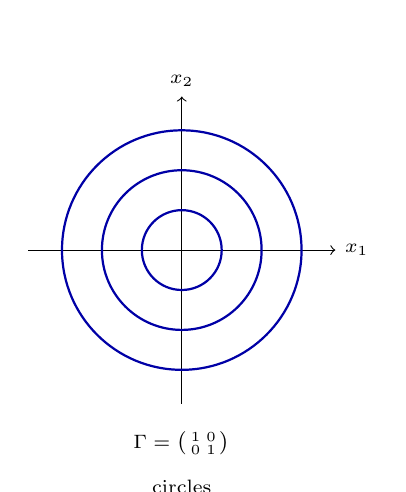
\begin{tikzpicture}[scale=0.78]
  \draw[->] (-2.5,0) -- (2.5,0) node[right,font=\scriptsize] {$x_{1}$};
  \draw[->] (0,-2.5) -- (0,2.5) node[above,font=\scriptsize] {$x_{2}$};
  \foreach \r in {0.65,1.3,1.95} \draw[blue!65!black,thick] (0,0) circle (\r);
  \node[font=\scriptsize] at (0,-3.15)
    {$\Gamma = \left(\begin{smallmatrix} 1 & 0 \\ 0 & 1 \end{smallmatrix}\right)$};
  \node[font=\scriptsize] at (0,-3.85) {circles};
\end{tikzpicture}
\hspace{0.7cm}
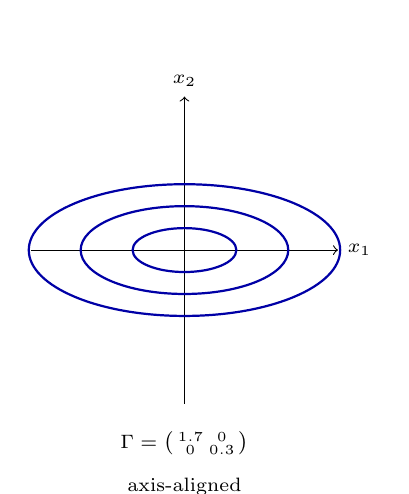
\begin{tikzpicture}[scale=0.78]
  \draw[->] (-2.5,0) -- (2.5,0) node[right,font=\scriptsize] {$x_{1}$};
  \draw[->] (0,-2.5) -- (0,2.5) node[above,font=\scriptsize] {$x_{2}$};
  \foreach \k in {0.65,1.3,1.95}
    \draw[blue!65!black,thick] (0,0) ellipse ({1.30*\k} and {0.55*\k});
  \node[font=\scriptsize] at (0,-3.15)
    {$\Gamma = \left(\begin{smallmatrix} 1.7 & 0 \\ 0 & 0.3 \end{smallmatrix}\right)$};
  \node[font=\scriptsize] at (0,-3.85) {axis-aligned};
\end{tikzpicture}
\hspace{0.7cm}
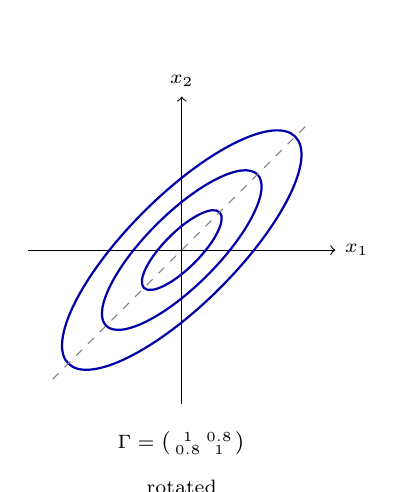
\begin{tikzpicture}[scale=0.78]
  \draw[->] (-2.5,0) -- (2.5,0) node[right,font=\scriptsize] {$x_{1}$};
  \draw[->] (0,-2.5) -- (0,2.5) node[above,font=\scriptsize] {$x_{2}$};
  \foreach \k in {0.65,1.3,1.95}
    \draw[blue!65!black,thick,rotate=45] (0,0) ellipse ({1.34*\k} and {0.45*\k});
  \draw[gray,dashed] (-2.1,-2.1) -- (2.1,2.1);
  \node[font=\scriptsize] at (0,-3.15)
    {$\Gamma = \left(\begin{smallmatrix} 1 & 0.8 \\ 0.8 & 1 \end{smallmatrix}\right)$};
  \node[font=\scriptsize] at (0,-3.85) {rotated};
\end{tikzpicture}

\vspace{0.9cm}

{\centering \small \textit{Level sets of a centrée bivariate Gaussian densité at
three matrices de covariance. The axes of the ellipses are the eigenvectors of
$\Gamma$ and their half-lengths are proportional to the square roots of its
eigenvalues; the dashed line in the third panel is the direction of largest
variance, which rotates away from the coordinate axes exactly when the
off-diagonal term is non-zero.}\par}
\end{figure}

\subsection{Définition}

Soit $n \geq 1$ un entier.

\begin{definition}[Vecteur gaussien]
Un vecteur aléatoire $X$ de dimension $n$ est un \textbf{vecteur gaussien}
(\textit{Gaussian vector}) si pour tout $a \in \reals^{n}$, la variable
aléatoire réelle $a^{T}X$ suit une loi gaussienne.
\end{definition}

Read that once more, because it is the whole chapter. The condition is on
\emph{every} linear combination of the components, not on the components. It is
not the definition a reader expects, which would be:

\begin{center}
\emph{(wrong)} $X$ is a vecteur gaussien when each component $X_{1},\dots,X_{n}$
follows a loi normale.
\end{center}

That condition is strictly weaker. It is implied by the real definition --- take
$a$ to be the $i$-th unit vector and $a^{T}X = X_{i}$ --- but it does not imply
it, and the counter-example below exhibits a pair of variables of loi normale
centrée réduite whose loi jointe is not Gaussian. Everything this chapter proves
is false under the weaker condition, so the distinction is not pedantry: it is
the hypothesis every theorem below is checked against.\\

Un vecteur gaussien a nécessairement une espérance et une matrice de covariance.
Il suffit de prendre pour $a$ les vecteurs unitaires de $\reals^{n}$: that makes
each component a normal variable, and a normal variable has moments of every
order, so no integrability hypothesis ever has to be added to a statement about
vecteurs gaussiens. Si $X$ est un vecteur gaussien d'espérance $\mu$ et de
matrice de covariance $\Gamma$, alors pour tout $a \in \reals^{n}$, la variable
aléatoire $a^{T}X$ suit une loi gaussienne d'espérance et de variance :
\[
  \expec(a^{T}X) = a^{T}\mu, \qquad
  \Var(a^{T}X) = \Cov(a^{T}X, a^{T}X) = a^{T}\Cov(X)\,a = a^{T}\Gamma a .
\]
In particular $a^{T}\Gamma a \geq 0$ for every $a$: the matrice de covariance of
a vecteur gaussien is symétrique and positive semi-definite, as any matrice de
covariance is. It need not be invertible, and the densité section below is about
what invertibility buys.

\begin{theorem}[Fonction caractéristique d'un vecteur gaussien]
Un vecteur gaussien $X$ d'espérance $\mu$ et de matrice de covariance $\Gamma$ a
pour fonction caractéristique :
\[
  \forall t \in \reals^{n}, \qquad
  \varphi_{X}(t) = e^{it^{T}\mu}\, e^{-\frac{t^{T}\Gamma t}{2}} .
\]
\end{theorem}

\begin{remark}
One line, and it is the reason the definition is stated over all linear
combinations. Pour tout $t \in \reals^{n}$, la variable aléatoire $t^{T}X$ suit
une loi gaussienne d'espérance $t^{T}\mu$ et de variance $t^{T}\Gamma t$, by
definition, so evaluating its one-dimensional fonction caractéristique at the
single point $1$ gives
\[
  \varphi_{X}(t) = \expec\!\left(e^{it^{T}X}\right) = \varphi_{t^{T}X}(1)
                 = e^{it^{T}\mu}e^{-\frac{t^{T}\Gamma t}{2}} ,
\]
the last equality being the proposition above on the fonction caractéristique
de la loi normale. A definition by lois marginales
would give this at the $n$ unit vectors only, which is not enough to know the
joint fonction caractéristique.
\end{remark}

\begin{notation}
Since the fonction caractéristique determines the loi, la loi d'un vecteur
gaussien est entièrement caractérisée par son espérance et sa matrice de
covariance. On notera $X \sim \mathcal{N}(\mu,\Gamma)$ un vecteur gaussien
d'espérance $\mu$ et de matrice de covariance $\Gamma$. The reuse of the symbol
$\Gamma$ here is one of the deliberate collisions chapter 2 sets out.
\end{notation}

This is the practical content of the chapter. To identify the loi of
anything built from a vecteur gaussien, it suffices to check that the thing is
Gaussian and then to compute two objects, a mean vector and a matrice de
covariance. No densité, no integral, no convolution.

\begin{example}[Reading off the loi of a projection]
Soit $X$ un vecteur gaussien, with
\[
  \mu = \begin{pmatrix} 2 \\ 1 \end{pmatrix}, \qquad
  \Gamma = \begin{pmatrix} 2 & -1 \\ -1 & 3 \end{pmatrix}, \qquad
  a = \begin{pmatrix} 1 \\ -1 \end{pmatrix} .
\]
The variable $a^{T}X = X_{1} - X_{2}$ est une variable aléatoire de loi
gaussienne, comme projection d'un vecteur gaussien --- by definition --- so only
its two parameters are left to compute:
\[
  \expec(a^{T}X) = a^{T}\mu = 2 - 1 = 1, \qquad
  \Var(a^{T}X) = a^{T}\Gamma a = 2 - (-1) - (-1) + 3 = 7 .
\]
Hence $a^{T}X \sim \mathcal{N}(1,7)$. The whole computation is the expansion
$a^{T}\Gamma a = \Gamma_{11} - \Gamma_{12} - \Gamma_{21} + \Gamma_{22}$, and the
two off-diagonal terms are counted twice precisely because $\Gamma$ is symétrique.
\end{example}

\subsection{Construction d'un vecteur gaussien}

Soit $Z$ un vecteur aléatoire dont les composantes sont $n$ variables aléatoires
i.i.d.\ de loi normale centrée réduite. Il est facile de voir que $Z$ est un
vecteur gaussien, by indépendance :
\[
  \forall t \in \reals^{n}, \qquad
  \varphi_{Z}(t) = \expec\!\left(e^{it^{T}Z}\right)
                 = \varphi_{Z_{1}}(t_{1}) \dots \varphi_{Z_{n}}(t_{n})
                 = e^{-\frac{\|t\|^{2}}{2}} ,
\]
which is the fonction caractéristique of the previous section with $\mu = 0$ and
$\Gamma = I_{n}$. L'espérance de $Z$ est nulle et sa matrice de covariance est la
matrice identité : sa loi est dite \textbf{centrée réduite}
(\textit{standard}).
Les transformations affines de $Z$ permettent de construire n'importe quel
vecteur gaussien.

\begin{prop}
Pour toute matrice $A$ de taille $n \times n$ et tout vecteur $\mu$ de dimension
$n$, le vecteur aléatoire $X = AZ + \mu$ est un vecteur gaussien d'espérance
$\mu$ et de matrice de covariance $\Gamma = AA^{T}$.
\end{prop}

\begin{remark}
Pour tout $a \in \reals^{n}$, la variable aléatoire
$a^{T}X = (A^{T}a)^{T}Z + a^{T}\mu$, qui est la projection d'un vecteur
gaussien, suivie d'une translation, suit une loi gaussienne. Le vecteur aléatoire
$X$ est donc gaussien, by definition. Son espérance et sa matrice de covariance
sont données par
$\expec(X) = A\expec(Z) + \mu = \mu$ and
$\Cov(X) = \Cov(AZ) = A\Cov(Z)A^{T} = AA^{T}$, by linearity of the espérance and
bilinearity of the covariance.
\end{remark}

\begin{remark}
The construction reaches every vecteur gaussien, not just some. A matrice de
covariance $\Gamma$ is symétrique and positive semi-definite, so it has a spectral
decomposition $\Gamma = UDU^{T}$ with $U$ orthogonal and $D$ diagonal with
non-negative entries; taking $A = UD^{1/2}$ gives $AA^{T} = \Gamma$. So for every
$\mu$ and every symétrique positive semi-definite $\Gamma$ there is a vecteur
gaussien $\mathcal{N}(\mu,\Gamma)$, and it can always be realised as $AZ + \mu$
with $Z$ centré réduit. Positive semi-definiteness is the whole condition --- a
symétrique matrix that fails it is not the matrice de covariance of anything.
\end{remark}

\begin{example}[Which matrices de covariance are admissible]
Soit $X$ un vecteur gaussien centré de dimension $2$ et de matrice de covariance
\[
  \Gamma = \begin{pmatrix} 1 & 1 \\ 1 & \alpha \end{pmatrix} .
\]
For $\Gamma$ to be a matrice de covariance, la matrice doit être semi-définie
positive. A symétrique $2 \times 2$ matrix is positive semi-definite exactly when
its two diagonal entries and its determinant are all non-negative. Here those
three quantities are $\Gamma_{11} = 1$, $\Gamma_{22} = \alpha$ and
$\det\Gamma = \alpha - 1$, so the conditions read $\alpha \geq 0$ together with
$\alpha \geq 1$, and il faut et il suffit d'avoir $\alpha \geq 1$ --- the
determinant condition is the binding one and it subsumes the condition on the
second diagonal entry. The boundary case $\alpha = 1$ is the dégénéré
one: there $\det\Gamma = 0$, the vector is carried by a line, and the densité
theorem below says it has no densité. For $\alpha > 1$ it does, and les
composantes ne sont pas indépendantes, whatever $\alpha$ is, since the
off-diagonal entry is $1 \neq 0$ --- leur coefficient de corrélation est
$1/(\sqrt{1}\sqrt{\alpha}) = 1/\sqrt{\alpha}$, which tends to $0$ but never
reaches it.
\end{example}

\subsection{Un contre-exemple}

Les composantes d'un vecteur gaussien suivent des lois gaussiennes : il suffit de
projeter le vecteur sur chaque vecteur unitaire de $\reals^{n}$. La réciproque
n'est pas vraie. Nous donnons ici un exemple de vecteur aléatoire dont les
composantes suivent des lois gaussiennes mais qui n'est pas gaussien. It is the
reason the definition above is stated over all linear combinations, and it is
worth carrying with its computation rather than as an assertion, because the
computation is short and because the same shape recurs.\\

Soit $Z$ une variable aléatoire suivant une loi normale centrée réduite et $Y$
une variable aléatoire discrète, indépendante de $Z$, qui vaut $1$ avec
probabilité $\tfrac{1}{2}$ et $-1$ sinon. On vérifie facilement que $YZ$ suit une
loi gaussienne. Conditioning on the two values of $Y$ and using indépendance,
\[
  \forall t \in \reals, \qquad
  \varphi_{YZ}(t) = \expec\!\left(e^{iYZt}\right)
                  = \tfrac{1}{2}\expec\!\left(e^{iZt}\right)
                    + \tfrac{1}{2}\expec\!\left(e^{-iZt}\right)
                  = \tfrac{1}{2}\varphi_{Z}(t) + \tfrac{1}{2}\varphi_{Z}(-t)
                  = \varphi_{Z}(t) ,
\]
the last equality because $\varphi_{Z}(t) = e^{-t^{2}/2}$ is even. By injectivity
of the fonction caractéristique, $YZ \sim \mathcal{N}(0,1)$.\\

Le vecteur $X = (Z, YZ)$, dont les composantes suivent des lois gaussiennes (both
of them the loi normale centrée réduite), n'est pas gaussien. En effet, sa
projection sur le vecteur $a = (1,1)$ --- the variable $a^{T}X = Z + YZ$ ---
satisfies
\[
  \prob(Z + YZ = 0) = \prob(Y = -1) = \tfrac{1}{2} ,
\]
since $Z + YZ = 0$ on the événement $\{Y = -1\}$. A loi normale can put mass
$\tfrac{1}{2}$ on a single point only if it is a Dirac mass, that is only if
$\sigma = 0$ under the Dirac convention above; and $Z + YZ$ is not presque
sûrement $0$, because on the événement $\{Y = 1\}$, of probability $\tfrac{1}{2}$,
it equals $2Z \sim \mathcal{N}(0,4)$. So $Z + YZ$ is neither a variable with a
normal densité nor a Dirac mass, hence not normal, hence $X$ is not a vecteur
gaussien.\\

Pour qu'un vecteur aléatoire dont les composantes suivent des lois gaussiennes
soit gaussien, il faut des conditions supplémentaires, comme l'indépendance de
ses composantes, as the concatenation corollary below shows.

\begin{remark}
The same pair says something sharper, and it is the reason to keep it in view
when reading the indépendance theorem below. The two components are
\emph{décorrélées}:
\[
  \Cov(Z, YZ) = \expec(Z \cdot YZ) - \expec(Z)\expec(YZ)
              = \expec(Y)\expec(Z^{2}) - 0 = 0 ,
\]
using the indépendance of $Y$ and $Z$ and $\expec(Y) = 0$. They are very far from
independent, since $|YZ| = |Z|$ makes each one a function of the other's absolute
value. Two variables of loi normale centrée réduite, décorrélées, not
independent. Nothing is wrong: the indépendance theorem below, the one that turns
zero covariance into indépendance, has the hypothesis that the pair is a vecteur
gaussien, and this pair is not.
\end{remark}

\begin{figure}[ht]
\centering
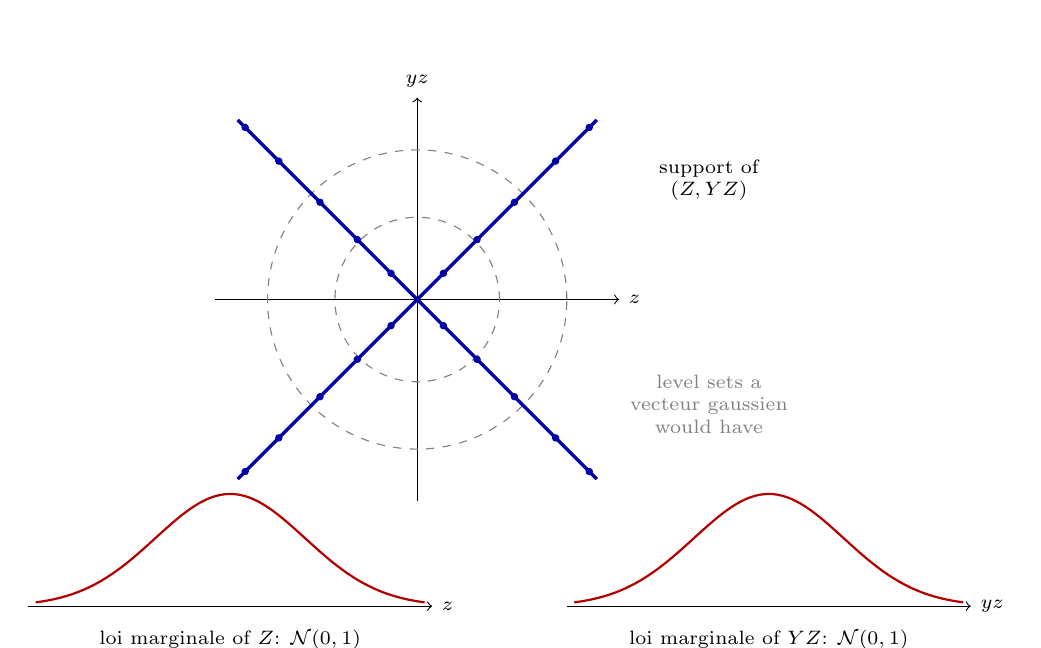
\begin{tikzpicture}[scale=0.95]
  \draw[->] (-2.7,0) -- (2.7,0) node[right,font=\scriptsize] {$z$};
  \draw[->] (0,-2.7) -- (0,2.7) node[above,font=\scriptsize] {$yz$};
  \draw[gray,dashed] (0,0) circle (1.1);
  \draw[gray,dashed] (0,0) circle (2.0);
  \draw[very thick,blue!65!black] (-2.4,-2.4) -- (2.4,2.4);
  \draw[very thick,blue!65!black] (-2.4,2.4) -- (2.4,-2.4);
  \foreach \s in {0.35,0.8,1.3,1.85,2.3}
    {\fill[blue!65!black] (\s,\s) circle (0.05);
     \fill[blue!65!black] (-\s,-\s) circle (0.05);
     \fill[blue!65!black] (\s,-\s) circle (0.05);
     \fill[blue!65!black] (-\s,\s) circle (0.05);}
  \node[font=\scriptsize,align=center] at (3.9,1.6)
    {support of\\$(Z,YZ)$};
  \node[font=\scriptsize,align=center,gray] at (3.9,-1.4)
    {level sets a\\vecteur gaussien\\would have};
  \begin{scope}[xshift=-2.5cm,yshift=-4.1cm]
    \draw[->] (-2.7,0) -- (2.7,0) node[right,font=\scriptsize] {$z$};
    \draw[thick,red!70!black,smooth,samples=80,domain=-2.6:2.6]
      plot (\x,{1.5*exp(-\x*\x/2)});
    \node[font=\scriptsize] at (0,-0.45) {loi marginale of $Z$: $\mathcal{N}(0,1)$};
  \end{scope}
  \begin{scope}[xshift=4.7cm,yshift=-4.1cm]
    \draw[->] (-2.7,0) -- (2.7,0) node[right,font=\scriptsize] {$yz$};
    \draw[thick,red!70!black,smooth,samples=80,domain=-2.6:2.6]
      plot (\x,{1.5*exp(-\x*\x/2)});
    \node[font=\scriptsize] at (0,-0.45) {loi marginale of $YZ$: $\mathcal{N}(0,1)$};
  \end{scope}
\end{tikzpicture}

{\centering \small \textit{The counter-example. Both lois marginales are the bell
curve of the loi normale centrée réduite, yet the loi jointe sits on the union of
the two diagonals and is visibly not elliptical --- it is carried by a set
négligeable pour la mesure de Lebesgue, so it has no densité at all. The dashed
circles show the level sets the loi jointe would have had if the pair were a
vecteur gaussien with these lois marginales and zero covariance.}\par}
\end{figure}

\subsection{Existence d'une densité}

A vecteur gaussien always has a loi, a fonction caractéristique and
moments of every order. Whether it has a \emph{densité} is a separate question,
and the answer is a single linear-algebra condition.

\begin{theorem}[Densité d'un vecteur gaussien]
Un vecteur gaussien $X$ d'espérance $\mu$ et de matrice de covariance $\Gamma$ a
une densité par rapport à la mesure de Lebesgue si et seulement si $\Gamma$ est
inversible. Cette densité est alors donnée par :
\[
  \forall x \in \reals^{n}, \qquad
  f_{X}(x) = \frac{1}{(2\pi)^{\frac{n}{2}}\sqrt{\det\Gamma}}\,
             e^{-\frac{1}{2}(x-\mu)^{T}\Gamma^{-1}(x-\mu)} .
\]
\end{theorem}

\begin{proof}
Comme $\Gamma$ est symétrique et positive, il existe une matrice $A$ de taille
$n \times n$ telle que $\Gamma = AA^{T}$. By the previous section, on peut donc
écrire $X = AZ + \mu$ avec $Z$ un vecteur gaussien centré réduit de dimension
$n$. Ce vecteur a pour densité :
\[
  \forall z \in \reals^{n}, \qquad
  f_{Z}(z) = \frac{1}{(2\pi)^{\frac{n}{2}}}\, e^{-\frac{\|z\|^{2}}{2}} .
\]
By the théorème de transfert, pour toute fonction mesurable positive $\phi$, on
a :
\[
  \expec(\phi(X)) = \expec(\phi(AZ + \mu))
    = \int \phi(Az + \mu)\, \frac{1}{(2\pi)^{\frac{n}{2}}}\,
      e^{-\frac{\|z\|^{2}}{2}}\, dz .
\]

Si $\Gamma$ est inversible, $A$ l'est aussi, since $\det\Gamma = (\det A)^{2}$,
et l'application $z \mapsto Az + \mu$ est un difféomorphisme de $\reals^{n}$ onto
itself, de matrice jacobienne $A$, which is constant. On obtient par changement
de variable $x = Az + \mu$, whose inverse is $z = A^{-1}(x-\mu)$ and whose
Jacobian factor is $|\det A|$ :
\[
  \expec(\phi(X)) = \int \phi(x)\, \frac{1}{(2\pi)^{\frac{n}{2}}}\,
    e^{-\frac{1}{2}(x-\mu)^{T}(A^{-1})^{T}A^{-1}(x-\mu)}\,
    \frac{dx}{|\det A|} .
\]
Now $(A^{-1})^{T}A^{-1} = (AA^{T})^{-1} = \Gamma^{-1}$ and
$|\det A| = \sqrt{\det\Gamma}$; on en déduit le résultat attendu --- the
integrand is the announced densité and $X$ has that densité, the function $\phi$
being an arbitrary positive mesurable fonction test.\\

Si $\Gamma$ n'est pas inversible, $A$ ne l'est pas non plus et il existe un
vecteur $u \in \reals^{n}$ non nul tel que $u^{T}A = 0$. For that
$u$,
\[
  u^{T}(X - \mu) = u^{T}AZ = 0 \qquad \text{almost surely}, \qquad \text{hence}
  \qquad \prob\!\left(u^{T}(X-\mu) = 0\right) = 1 .
\]
L'hyperplan $\{x \in \reals^{n} : u^{T}(x - \mu) = 0\}$ de $\reals^{n}$ est
négligeable pour la mesure de Lebesgue. A vecteur aléatoire with a densité gives
probability zero to every set négligeable pour la mesure de Lebesgue, so le
vecteur $X$ ne peut avoir de densité.
\end{proof}

The second half of the proof is not a technicality to be skipped, and the vectors
it describes are not error cases. When $\Gamma$ is singular of rank $r < n$, the
vector $X$ is carried by the affine subspace $\mu + \operatorname{im}(A)$ of
dimension $r$: it is a genuine vecteur gaussien, its fonction caractéristique is
still $e^{it^{T}\mu}e^{-t^{T}\Gamma t/2}$, its loi is still determined by
$\mu$ and $\Gamma$, and along the $n-r$ directions in the kernel it is deterministic.
Such a vector is called \textbf{dégénéré} (\textit{degenerate}). It simply has no
densité on $\reals^{n}$ --- though it does have one on the subspace that carries
it, once that subspace is identified with $\reals^{r}$. Vecteurs gaussiens
dégénérés turn up on their own in exam problems, most often as a residual vector
after a projection, so the right reflex on being asked for a densité is to
compute $\det\Gamma$ first.

\begin{figure}[ht]
\centering
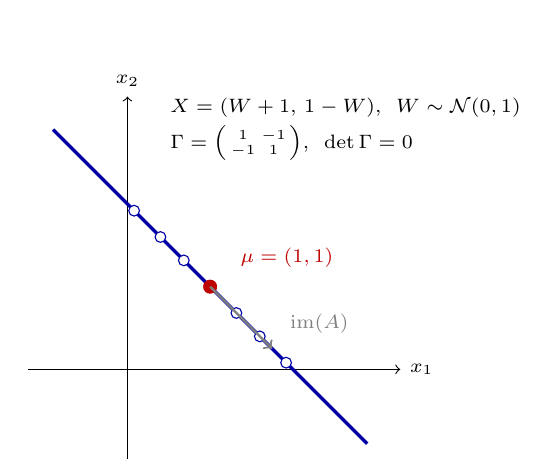
\begin{tikzpicture}[scale=1.05]
  \draw[->] (-1.2,0) -- (3.3,0) node[right,font=\scriptsize] {$x_{1}$};
  \draw[->] (0,-1.2) -- (0,3.3) node[above,font=\scriptsize] {$x_{2}$};
  \draw[very thick,blue!65!black] (-0.9,2.9) -- (2.9,-0.9);
  \foreach \s in {-1.3,-0.85,-0.45,0.45,0.85,1.3}
    \draw[blue!65!black,fill=white,thin]
      ({1+0.707*\s},{1-0.707*\s}) circle (0.065);
  \fill[red!75!black] (1,1) circle (0.085);
  \node[font=\scriptsize,red!75!black,anchor=west] at (1.25,1.35) {$\mu = (1,1)$};
  \draw[->,gray,thick] (1,1) -- (1.75,0.25);
  \node[font=\scriptsize,gray,anchor=west] at (1.85,0.55) {$\operatorname{im}(A)$};
  \node[font=\scriptsize,align=left,anchor=west] at (0.4,2.9)
    {$X = (W+1,\, 1-W)$, \ $W \sim \mathcal{N}(0,1)$\\[2pt]
     $\Gamma = \left(\begin{smallmatrix} 1 & -1 \\ -1 & 1 \end{smallmatrix}\right)$,
     \ $\det\Gamma = 0$};
\end{tikzpicture}

{\centering \small \textit{A vecteur gaussien dégénéré in $\reals^{2}$: all its
mass lies on the line $x_{1} + x_{2} = 2$, which is négligeable pour la mesure de
Lebesgue, so there is no densité on the plane. The loi is still Gaussian, still
determined by $\mu$ and $\Gamma$, and on the line itself it is a one-dimensional
$\mathcal{N}(0,2)$ about $\mu$.}\par}
\end{figure}

\begin{example}[Two vectors built from one normal variable]
Soit $W \sim \mathcal{N}(0,1)$ une variable aléatoire de loi normale centrée
réduite --- a single one. The vector
$(W, 2W, 3W)$ is Gaussian: any linear combination
$a_{1}W + 2a_{2}W + 3a_{3}W = (a_{1}+2a_{2}+3a_{3})W$ is a scalar multiple of
$W$, hence normal --- including the case where the scalar vanishes, which is the
Dirac mass at $0$ and is normal by convention. Its mean is $0$ and its matrice
de covariance is
\[
  \Gamma = \begin{pmatrix} 1 & 2 & 3 \\ 2 & 4 & 6 \\ 3 & 6 & 9 \end{pmatrix} ,
\]
of rank $1$, hence singular: no densité. The vector lives on the line spanned by
$(1,2,3)$, which is what rank $1$ says.\\

The vector $(W+1, 1-W)$ is Gaussian for the same reason, with mean $(1,1)$ and
matrice de covariance
\[
  \Gamma = \begin{pmatrix} 1 & -1 \\ -1 & 1 \end{pmatrix} ,
  \qquad \det\Gamma = 0 .
\]
Again no densité: the two components sum to $2$ presque sûrement, so the vector
is carried by the line $x_{1} + x_{2} = 2$. This is the vector drawn in the
figure above.
\end{example}

\begin{example}[Recognising a vecteur gaussien from its densité]
Soit $(X,Y)$ un vecteur aléatoire de densité :
\[
  \forall x,y \in \reals, \qquad
  f_{X,Y}(x,y) = c\,\exp\!\left(-\tfrac{1}{8}\left(3x^{2} + 2xy + 3y^{2}\right)\right) ,
\]
avec $c$ une constante strictement positive. The exponent is a negative definite
quadratic form with no linear part, so the theorem above identifies the
loi by matching coefficients: the vector is a vecteur gaussien centré with
\[
  \tfrac{1}{2}\begin{pmatrix} x \\ y \end{pmatrix}^{T} \Gamma^{-1}
  \begin{pmatrix} x \\ y \end{pmatrix}
  = \tfrac{1}{8}\left(3x^{2} + 2xy + 3y^{2}\right)
  \quad\Longrightarrow\quad
  \Gamma^{-1} = \tfrac{1}{4}\begin{pmatrix} 3 & 1 \\ 1 & 3 \end{pmatrix} ,
\]
the off-diagonal entries of $\Gamma^{-1}$ each carrying half of the cross term
$2xy$ because the form is symétrique. Inverting,
\[
  \Gamma = 4 \cdot \frac{1}{8}\begin{pmatrix} 3 & -1 \\ -1 & 3 \end{pmatrix}
         = \frac{1}{2}\begin{pmatrix} 3 & -1 \\ -1 & 3 \end{pmatrix},
  \qquad \det\Gamma = \frac{9-1}{4} = 2 ,
\]
so the normalising constant is forced:
$c = 1/\left(2\pi\sqrt{\det\Gamma}\right) = 1/(2\pi\sqrt{2})$. The lois
marginales are read off the diagonal, $X \sim \mathcal{N}(0,\tfrac{3}{2})$ and
$Y \sim \mathcal{N}(0,\tfrac{3}{2})$, and the components are not independent
since $\Gamma$ is not diagonal --- their coefficient de corrélation is
$(-\tfrac{1}{2})/(\tfrac{3}{2}) = -\tfrac{1}{3}$.
\end{example}

\subsection{Propriétés}

Nous terminons par quelques propriétés utiles des vecteurs gaussiens --- the
properties that do the work in practice. The first is the one almost every
exercise on this chapter starts from.

\begin{theorem}[Transformation affine]
Toute transformation affine d'un vecteur gaussien est un vecteur gaussien.
Precisely, if $X \sim \mathcal{N}(\mu,\Gamma)$ has dimension $n$, avec $A$
matrice de taille $m \times n$ et $b$ vecteur de dimension $m$, then
\[
  Y = AX + b \ \sim\ \mathcal{N}\!\left(A\mu + b,\ A\Gamma A^{T}\right) .
\]
\end{theorem}

\begin{remark}
The fonction caractéristique computes itself, and the computation is where the
transformed parameters come from:
\[
  \varphi_{Y}(t) = \expec\!\left(e^{it^{T}(AX+b)}\right)
                 = e^{it^{T}b}\,\varphi_{X}(A^{T}t)
                 = e^{it^{T}(A\mu + b)}\, e^{-\frac{1}{2}t^{T}A\Gamma A^{T}t} ,
\]
for $t \in \reals^{m}$. Il s'agit de la fonction caractéristique d'un vecteur
gaussien d'espérance $A\mu + b$ et de matrice de covariance $A\Gamma A^{T}$. Note
that $A$ need not be square and need not have full rank: $m$ may exceed $n$ or
fall short of it, and $A\Gamma A^{T}$ is then very often singular. That is fine,
and it is why the dégénéré case of the densité section had to be kept.
\end{remark}

This theorem is the workhorse. Any question of the form ``what is the
loi of this linear combination, this projection, this residual'' is
answered by writing the object as $AX + b$ and computing $A\mu + b$ and $A\Gamma A^{T}$.

\begin{theorem}[Indépendance des composantes]
Les composantes d'un vecteur gaussien sont indépendantes si et seulement si la
matrice de covariance de ce vecteur est diagonale.
\end{theorem}

\begin{remark}
By the fonction caractéristique theorem above, un vecteur gaussien $X$
d'espérance $\mu$ et de matrice de covariance $\Gamma$ a pour fonction
caractéristique $\varphi_{X}(t) = e^{it^{T}\mu}e^{-t^{T}\Gamma t/2}$. Chapter 6's
criterion says les composantes sont indépendantes si et seulement si cette
fonction s'écrit comme un produit of functions of the individual $t_{i}$. The
linear part $e^{it^{T}\mu}$ always
factorises; the quadratic part $t^{T}\Gamma t = \sum_{j,k}\Gamma_{jk}t_{j}t_{k}$
factorises exactly when it has no cross term, that is exactly when $\Gamma$ is
diagonal.
\end{remark}

\begin{remark}
Deux composantes d'un vecteur gaussien sont indépendantes si et seulement si leur
covariance est nulle. Il suffit en effet d'appliquer le résultat précédent au
vecteur aléatoire formé par ces deux composantes, qui est lui-même gaussien by
the affine transformation theorem --- extracting two coordinates is a linear map.
\end{remark}

\begin{remark}
The same computation covers \textbf{blocs} (\textit{blocks}), which is the form
used in the examples below. Split a vecteur gaussien $X$ into blocs
$X^{(1)},\dots,X^{(p)}$ of dimensions $n_{1},\dots,n_{p}$ and split $t$ the same
way. If $\Gamma$ is diagonal by blocs for that split, with diagonal blocs
$\Gamma^{(1)},\dots,\Gamma^{(p)}$ --- the diagonal blocs themselves being
arbitrary --- then
$t^{T}\mu = \sum_{k}(t^{(k)})^{T}\mu^{(k)}$ and
$t^{T}\Gamma t = \sum_{k}(t^{(k)})^{T}\Gamma^{(k)}t^{(k)}$, so
\[
  \varphi_{X}(t) = \prod_{k=1}^{p}
    e^{i(t^{(k)})^{T}\mu^{(k)}}\,
    e^{-\frac{1}{2}(t^{(k)})^{T}\Gamma^{(k)}t^{(k)}}
  = \prod_{k=1}^{p} \varphi_{X^{(k)}}\!\left(t^{(k)}\right) ,
\]
each factor being the fonction caractéristique of the bloc $X^{(k)}$, which is
Gaussian with mean $\mu^{(k)}$ and matrice de covariance $\Gamma^{(k)}$ by the
affine transformation theorem. Chapter 6's comparison-vector argument for the
characterisation of indépendance never uses that the pieces are scalar: run it
with blocs in place of components and this factorisation gives that
$X^{(1)},\dots,X^{(p)}$ are independent. The converse is the same computation
read backwards. So two blocs of a vecteur gaussien are independent as soon as the
cross-covariance bloc between them vanishes, and this \textbf{bloc form} of the
theorem is what is meant below whenever a cross bloc is computed and found to be
zero. The componentwise statement is the case where every bloc has size one.
\end{remark}

\begin{remark}
This is the one place in the whole course where a zero covariance gives
indépendance, and it is worth saying loudly because the temptation to reuse it is
permanent. In general, being décorrélées does not mean being independent:
chapter 1's correlation figure shows two variables with covariance zero and an
obvious functional dependence between them, and the counter-example above gives a
second instance
with both lois marginales centrées réduites. The hypothesis that rescues the
implication here is not that the components are normal --- the counter-example's
components are normal --- but that the \emph{vector} is Gaussian, that is that
every linear combination of the components is normal. Check that hypothesis
before using this theorem; it is the single most common way to go wrong on this
chapter.
\end{remark}

\begin{example}[Independent and dependent pairs of linear combinations]
Soit $X$ et $Y$ deux variables aléatoires indépendantes de même loi normale
centrée réduite. The vector $(X,Y)$ is
Gaussian --- independent normal components, by the corollary below --- and so is
every linear image of it. Les vecteurs associés étant gaussiens, il suffit de
regarder la corrélation: each question is a covariance computation.\\

For $X+Y$ and $X-Y$: the pair is a linear image of $(X,Y)$, hence a vecteur
gaussien, and
$\Cov(X+Y, X-Y) = \Var(X) - \Var(Y) = 1 - 1 = 0$, donc indépendantes.\\

For $X+2Y$ and $X-Y$: again a vecteur gaussien, but
$\Cov(X+2Y, X-Y) = \Var(X) - 2\Var(Y) = 1 - 2 = -1 \neq 0$, donc dépendantes.
Note that both variables are normal in both cases; it is the
covariance, not the lois marginales, that decides.
\end{example}

\begin{theorem}[Somme]
La somme de vecteurs gaussiens indépendants est un vecteur gaussien. Precisely,
soit $X^{(1)},\dots,X^{(m)}$ des vecteurs gaussiens indépendants de dimension $n$.
Write $\mu^{(k)}$ for the mean and $\Gamma^{(k)}$ for the matrice de covariance
of $X^{(k)}$. Then leur somme $X$ est un vecteur gaussien d'espérance
$\mu^{(1)} + \dots + \mu^{(m)}$ et de matrice de covariance
$\Gamma^{(1)} + \dots + \Gamma^{(m)}$.
\end{theorem}

\begin{remark}
By indépendance the fonction caractéristique of the sum is the product of the
fonctions caractéristiques, and multiplying the exponentials adds the means in
the linear part and adds the matrices de covariance in the quadratic part:
\[
  \varphi_{X}(t) = \varphi_{X^{(1)}}(t) \dots \varphi_{X^{(m)}}(t)
    = e^{it^{T}\left(\mu^{(1)}+\dots+\mu^{(m)}\right)}
      e^{-\frac{1}{2}t^{T}\left(\Gamma^{(1)}+\dots+\Gamma^{(m)}\right)t} .
\]
Indépendance is essential: without it the product formula fails, and the sum of
two dependent vecteurs gaussiens need not be Gaussian at all.
\end{remark}

\begin{corollary}[Concatenation]
La concatenation de vecteurs gaussiens indépendants est un vecteur gaussien.
\end{corollary}

\begin{remark}
La projection du vecteur formé par cette concatenation sur un vecteur quelconque
est la somme de variables aléatoires gaussiennes indépendantes, one projection
per bloc, which is normal by the previous theorem. Its matrice de covariance is
diagonal by blocs, the blocs being the matrices de covariance of the pieces,
which by the bloc form of the indépendance theorem is consistent: the blocs are
independent of one another.
\end{remark}

En particulier, un vecteur dont les composantes suivent des lois gaussiennes
\emph{et sont indépendantes} est gaussien ; sans la condition d'indépendance, le
résultat est faux --- that is exactly the counter-example above, whose components
are normal, décorrélées, and not independent.

\begin{example}[A difference of two independent vecteurs gaussiens]
Soit $X$ et $Y$ deux vecteurs gaussiens indépendants de mêmes espérance $\mu$ et
matrice de covariance $\Gamma$. Then $-2Y \sim \mathcal{N}(-2\mu, 4\Gamma)$ by
the affine transformation theorem, the factor $4$ being $(-2)\Gamma(-2)^{T}$, and
$X$ and $-2Y$ are independent, so by the sum theorem
\[
  X - 2Y \ \sim\ \mathcal{N}\!\left(-\mu,\ 5\Gamma\right) .
\]
The trap the factor $4$ guards against is writing $\Gamma - 2\Gamma$ or
$\Gamma + 2\Gamma$: covariance is quadratic, so a scalar multiplier enters
squared.
\end{example}

\begin{example}[Two linear images of one standard vector]
Soit $Z$ un vecteur gaussien centré réduit de dimension $3$. On note $X = AZ$ et
$Y = BZ$ avec
\[
  A = \begin{pmatrix} 1 & 1 & 0 \\ 0 & 1 & 1 \\ 1 & 0 & -1 \end{pmatrix},
  \qquad
  B = \begin{pmatrix} 1 & -1 & 1 \end{pmatrix} .
\]
Ce sont des vecteurs gaussiens comme transformations linéaires d'un vecteur
gaussien --- centrés, with matrices de covariance $AA^{T}$ and $BB^{T}$:
\[
  X \sim \mathcal{N}\!\left(0,
    \begin{pmatrix} 2 & 1 & 1 \\ 1 & 2 & -1 \\ 1 & -1 & 2 \end{pmatrix}\right),
  \qquad
  Y \sim \mathcal{N}(0,3) .
\]
For indépendance, stack them: le vecteur $(X,Y)$ est lui-même gaussien comme
transformation linéaire --- the image of $Z$ under the $4 \times 3$
matrix whose first three rows are $A$ and whose last row is $B$ --- and the
cross-covariance bloc is $AB^{T}$. Computing row by row,
$(1,1,0)\cdot(1,-1,1) = 0$, $(0,1,1)\cdot(1,-1,1) = 0$ and
$(1,0,-1)\cdot(1,-1,1) = 0$, so $AB^{T} = 0$ and les variables $X$ et $Y$ sont
donc indépendantes --- by the bloc form of the indépendance theorem applied to
the stacked vecteur gaussien, which is the step that would be unavailable if the
stack were not Gaussian.\\

Note in passing that $\det A = 0$, since the first row of $A$ is the sum of the
other two, so $X_{1} = X_{2} + X_{3}$ presque sûrement and $X$ is a vecteur
gaussien dégénéré with no densité on $\reals^{3}$. Indépendance of $X$ and $Y$ is
untouched by that: the indépendance theorem asks about the matrice de covariance
only, never about a densité.
\end{example}

\begin{example}[Indépendance among three linear combinations]
Let $X$, $Y$, $Z$ be independent variables of loi normale centrée réduite, so that
$(X,Y,Z)$ is a vecteur gaussien centré réduit. Then
$T = X + Y + Z \sim \mathcal{N}(0,3)$, being a projection of it.\\

The pair $(T, X-Y)$ is a linear image of $(X,Y,Z)$, hence a vecteur gaussien, and
its parameters are
\[
  (T, X-Y) \sim \mathcal{N}\!\left(0,
    \begin{pmatrix} 3 & 0 \\ 0 & 2 \end{pmatrix}\right) ,
\]
the off-diagonal term being
$\Cov(X+Y+Z, X-Y) = \Var(X) - \Var(Y) = 0$. The matrice de covariance is
diagonal, so $T$ and $X-Y$ are independent; by symmetry of the roles of $X$, $Y$
and $Z$ the same holds for $Y-Z$ and for $Z-X$.\\

Now ask for which $\alpha$ the three variables $X+Y+Z$, $2X-Y-Z$ and $Y+\alpha Z$
are independent. The triple is again a linear image of $(X,Y,Z)$, so it is a
vecteur gaussien centré, with matrice de covariance
\[
  \begin{pmatrix}
    3 & 0 & 1+\alpha \\
    0 & 6 & -1-\alpha \\
    1+\alpha & -1-\alpha & 1+\alpha^{2}
  \end{pmatrix} .
\]
Indépendance holds if and only if this is diagonal, that is if and only if
$1 + \alpha = 0$, so $\alpha = -1$ is the only value. One scalar equation, no
densités, no integrals --- which is what the two theorems of this section buy.
\end{example}

\begin{example}[Conditioning one bloc of a vecteur gaussien on another]
This is the shape behind every Gaussian conditioning question, and it is the
affine transformation theorem followed by the indépendance theorem, in that
order.\\

Let $X$ and $Y$ be vecteurs aléatoires of dimensions $n$ and $m$ such that the
concatenation $(X,Y)$ is a vecteur gaussien centré with matrice de covariance
\[
  \Gamma = \begin{pmatrix} A & C \\ C^{T} & B \end{pmatrix} ,
\]
where the square blocs $A$ and $B$ have sizes $n \times n$ and $m \times m$, and
$A$ is invertible. Each bloc is a projection of a vecteur gaussien, so
$X \sim \mathcal{N}(0,A)$ and $Y \sim \mathcal{N}(0,B)$, and by the bloc form of
the indépendance theorem $X$ and $Y$ are independent if and only if $C = 0$.\\

For a general $m \times n$ matrix $M$, the vector $(X, Y - MX)$ is a linear image
of $(X,Y)$, hence a vecteur gaussien centré, and its matrice de covariance is
\[
  \begin{pmatrix}
    A & C - AM^{T} \\
    C^{T} - MA & B + MAM^{T} - MC - C^{T}M^{T}
  \end{pmatrix} .
\]
The cross bloc vanishes exactly when $C^{T} - MA = 0$, that is for
$M = C^{T}A^{-1}$ --- this is where the invertibility of $A$ is used, and it is
the only place it is needed. For that $M$, the bloc form of the indépendance
theorem makes $X$ and $Y - MX$ independent, and the espérance conditionnelle
follows without any further computation:
\[
  \expec(Y \mid X = x) = \expec(Y - MX \mid X = x) + \expec(MX \mid X = x)
                       = \expec(Y - MX) + Mx = Mx ,
\]
since $Y - MX$ is independent of $X$ and centré. The espérance conditionnelle of
one bloc of a vecteur gaussien centré given another is \emph{linear} in the
conditioning value, with matrix $C^{T}A^{-1}$.\\

Concretely, in dimension $1 + 1$: soit $X$ un vecteur gaussien centré de matrice
de covariance
\[
  \Gamma = \begin{pmatrix} 1 & 1 \\ 1 & 2 \end{pmatrix} .
\]
Here $A = 2$ is the variance of $X_{2}$ and $C^{T} = 1$ is the covariance, so
$M = \tfrac{1}{2}$ and $X_{1} - \tfrac{1}{2}X_{2}$ is independent of $X_{2}$. Its
variance is
$\Var(X_{1}) - \Cov(X_{1},X_{2}) + \tfrac{1}{4}\Var(X_{2})
 = 1 - 1 + \tfrac{1}{2} = \tfrac{1}{2}$, so
\[
  X_{1} \mid X_{2} = x_{2} \ \sim\
  \mathcal{N}\!\left(\tfrac{x_{2}}{2},\ \tfrac{1}{2}\right) ,
  \qquad
  \expec(X_{1} \mid X_{2}) = \tfrac{X_{2}}{2} \sim \mathcal{N}\!\left(0,\tfrac{1}{2}\right) .
\]
The conditional variance does not depend on $x_{2}$ --- another feature peculiar
to the Gaussian case. And conditioning on an événement rather than a value reduces to
a one-dimensional integral: with $X_{2} \sim \mathcal{N}(0,2)$ and
$\expec(X_{2} \mid X_{2} \geq 0) = \sigma\sqrt{2/\pi} = 2/\sqrt{\pi}$,
\[
  \expec(X_{1} \mid X_{2} \geq 0)
    = \tfrac{1}{2}\,\expec(X_{2} \mid X_{2} \geq 0) = \frac{1}{\sqrt{\pi}} .
\]
\end{example}

\begin{example}[Linear regression, and where the loi de Student comes from]
This assembles the whole chapter, and it is the shape a long exam problem takes.\\

Let $A$ be an $n \times d$ matrix with $n > d \geq 1$ and $A^{T}A$ invertible,
let $w$ be an unknown parameter vector of dimension $d$, and let $Z$ be a vecteur
gaussien centré of dimension $n$ with matrice de covariance $\sigma^{2}I_{n}$,
$\sigma^{2} > 0$. One observes
\[
  Y = Aw + Z \ \sim\ \mathcal{N}\!\left(Aw,\ \sigma^{2}I_{n}\right) ,
\]
by the affine transformation theorem. Write $P = A(A^{T}A)^{-1}A^{T}$ for the
orthogonal projection onto the column space of $A$, so that $P^{T} = P$ and
$P^{2} = P$, and set
\[
  W = (A^{T}A)^{-1}A^{T}Y, \qquad R = (I_{n} - P)Y .
\]
The stacked vector $(W,R)$ is a linear image of $Y$, hence a vecteur gaussien ---
that single sentence is the whole justification, and it is why the definition by
linear combinations is the useful one. Its mean is $(w, 0)$, since
$(A^{T}A)^{-1}A^{T}Aw = w$ and $(I_{n}-P)Aw = Aw - Aw = 0$, and its matrice de
covariance is diagonal by blocs:
\[
  \Cov\begin{pmatrix} W \\ R \end{pmatrix}
    = \sigma^{2}\begin{pmatrix} (A^{T}A)^{-1} & 0 \\ 0 & I_{n} - P \end{pmatrix} ,
\]
the cross bloc being
$\sigma^{2}(A^{T}A)^{-1}A^{T}(I_{n}-P) = \sigma^{2}(A^{T}A)^{-1}(A^{T} - A^{T}) = 0$
because $A^{T}P = A^{T}$. The bloc being zero, the bloc form of the
indépendance theorem gives that the estimator $W$ and the residual $R$ are
independent --- and in particular
so are the single component $W_{1}$ and the whole vector $R$.\\

Three consequences, each one of the theorems above. First,
$W_{1} \sim \mathcal{N}\!\left(w_{1},\, \sigma^{2}[(A^{T}A)^{-1}]_{11}\right)$,
read off the diagonal. Second, $R$ is a vecteur gaussien \emph{dégénéré}: its
matrice de covariance $\sigma^{2}(I_{n}-P)$ has rank $n-d$, so $R$ has no densité
on $\reals^{n}$, exactly as the densité theorem predicts. Third, writing
$\bar{Z} = Z/\sigma$ for the centré réduit part and using the spectral
decomposition of the projection $P$,
\[
  \frac{\|R\|^{2}}{\sigma^{2}} = \bar{Z}^{T}(I_{n}-P)\bar{Z}
\]
is a sum of the squares of $n-d$ independent variables of loi normale centrée
réduite, because $Q\bar{Z}$ is again a vecteur gaussien centré réduit for $Q$
orthogonal --- that is $QQ^{T} = I$ in the affine transformation theorem. It
therefore follows a loi du $\chi^{2}$ à $n-d$ degrés de liberté.\\

A variable of loi normale centrée réduite divided by the square root of an
independent $\chi^{2}$ over its degrees of freedom is by definition a variable of
\textbf{loi de Student} (\textit{Student distribution}), so
with $c = \sqrt{[(A^{T}A)^{-1}]_{11}}$,
\[
  \frac{W_{1} - w_{1}}{c\sqrt{\dfrac{\|R\|^{2}}{n-d}}}
\]
follows a loi de Student with $n-d$ degrees of freedom. The unknown
$\sigma$ has cancelled between numerator and denominator, which is the point of
the construction: the quantity can be computed from the data alone, and inverting
it around $w_{1}$ turns the symmetry of the loi de Student into a confidence
interval for the unknown parameter. Every step used only the two theorems of this
section --- an affine image of a vecteur gaussien is Gaussian, and a vanishing
covariance bloc in a vecteur gaussien is indépendance.
\end{example}

\begin{conclusion}
One definition carries the chapter: a vecteur aléatoire is Gaussian when every
linear combination of its components is a normal variable, and the counter-example
shows why nothing weaker will do. From it, the fonction caractéristique
$e^{it^{T}\mu}e^{-t^{T}\Gamma t/2}$ follows in a line, and with it the fact that
$\mu$ and $\Gamma$ determine the loi. The rest is arithmetic on those two
objects. An affine image $AX + b$ is Gaussian with parameters $A\mu + b$ and
$A\Gamma A^{T}$. A densité on $\reals^{n}$ exists exactly when $\Gamma$ is
invertible, and when it is not the vector is a perfectly good Gaussian carried by
an affine subspace. Components are independent exactly when $\Gamma$ is diagonal,
which makes this the one place in the course where zero covariance implies
indépendance --- and only because the vector, not merely each component, is
Gaussian.
\end{conclusion}

\section{Théorèmes limites}
Everything up to here has been about one variable aléatoire, or finitely many at
a time: its loi, its moments, its fonction caractéristique, the loi of a vector
built from it. Ce chapitre porte sur deux résultats fondamentaux de convergence
de suites de variables aléatoires : la loi des grands nombres et le théorème
central limite --- the two results the whole construction was built for. The loi
forte des grands nombres says that an empirical mean settles on the espérance,
and the théorème central limite that the error it makes on the way there is
Gaussian.\\
Both are statements that a sequence $X_{1}, X_{2}, \dots$ converges to
something, so both need a notion of convergence for variables aléatoires, and
there is more than one. A variable aléatoire is a function on $\Omega$, so one
can ask for convergence of the functions --- pointwise, for almost every
$\omega$ --- and that is the strongest thing to ask. Or one can forget $\Omega$
entirely and ask only that the \emph{lois} converge, which is much weaker and is
exactly what the théorème central limite delivers. Nous commençons par définir
deux notions usuelles de convergence d'une suite de variables aléatoires : la
convergence presque sûre et la convergence en loi. The first two subsections
below set them up and relate them; the last three are the theorems.

\begin{remark}
  D'autres notions de convergence existent, comme la convergence en
  probabilité, mais ne sont pas abordées
  dans ce cours --- convergence in $L^{p}$ is another. Convergence en
  probabilité is carried here anyway, marked as an addition, for the reason
  given at the end of the first subsection.
\end{remark}

\subsection{Convergence presque sûre}
Two French abbreviations run through this chapter, both already in use.
\textit{p.s.} is the probabilistic name for \textit{p.p.} from chapter 2,
specialised to a mesure that happens to be a probability --- the exceptional
set is $\prob$-négligeable rather than merely $\lambda$-négligeable, but nothing
else changes.\\
For an i.i.d.\ sequence both halves of the abbreviation are used in the proofs
below, and they are used differently --- indépendance gives the factorisation of
a fonction caractéristique or the vanishing of a cross term, and being
identiquement distribuées gives the single loi that the limit is expressed in
terms of. A sequence can have one without the other, and then neither theorem in
this chapter applies.

\begin{notation}
  Throughout, $X_{1}, X_{2}, \dots$ is a sequence of variables aléatoires réelles
  on a common espace de probabilité $(\Omega, \mathcal{F}, \prob)$, and
  $S_{n} = \sum_{i=1}^{n} X_{i}$ is its sequence of partial sums. That the space
  is common matters for convergence presque sûre, which compares
  $X_{n}(\omega)$ with $X(\omega)$ for the same $\omega$, and not at all for
  convergence en loi, which never looks at $\omega$.\\
  Two Greek letters are kept apart: $\varphi$ is a fonction caractéristique ---
  $\varphi_{X}$, $\varphi_{n}$, or a bare $\varphi$ for the limit's --- and
  $\phi$ is always a fonction test, bounded and continuous where convergence en
  loi is being tested, mesurable and non-negative where the théorème de
  transfert is being applied. A continuous map applied to a sequence is written
  $g$.
\end{notation}

La notion de convergence la plus forte est une convergence simple, valable pour
presque toute réalisation $\omega$: simple pointwise convergence of the
functions $X_{n} : \Omega \to \reals$, asked for not at every realisation but at
almost every one.

\begin{definition}[Convergence presque sûre (\textit{almost-sure convergence})]
  On dit qu'une suite de variables aléatoires réelles $X_{1}, X_{2}, \dots$
  converge \textbf{presque sûrement} vers une variable aléatoire réelle $X$ si
  la suite $X_{1}(\omega), X_{2}(\omega), \dots$ converge
  vers $X(\omega)$ pour presque tout $\omega \in \Omega$ :
  \[
    \prob\left(\left\{\omega \in \Omega : \lim_{n \to +\infty} X_{n}(\omega)
      = X(\omega)\right\}\right) = 1 .
  \]
\end{definition}

\begin{notation}
  On utilise la notation :
  \[
    X_{n} \cvas X .
  \]
\end{notation}

The set appearing in the definition is mesurable --- it is
$\bigcap_{k \geq 1} \bigcup_{N \geq 1} \bigcap_{n \geq N}
\{|X_{n} - X| \leq 1/k\}$, a countable combination of événements --- so asking
for its probability is legitimate. What the definition does \emph{not} require
is convergence at every $\omega$, and in most applications there is a genuine
exceptional événement: the binary-digit example below has one, and it contains
the dyadic rationals, whose expansions are eventually constant. It is
$\prob$-négligeable, but not for the cheap reason of being countable --- it is
not countable.

\begin{prop}
  Si $X_{n} \cvas X$, alors $g(X_{n}) \cvas g(X)$ pour toute fonction
  continue $g$.
\end{prop}

\begin{proof}
  Soit $\omega \in \Omega$ tel que $\lim_{n} X_{n}(\omega) = X(\omega)$. Pour
  toute fonction continue $g$,
  $\lim_{n} g(X_{n}(\omega)) = g(X(\omega))$, by continuity at the point
  $X(\omega)$. The événement on which $g(X_{n})$ converges to $g(X)$ therefore
  contains the événement on which $X_{n}$ converges to $X$. On a donc :
  \[
    \prob\left(\lim_{n} g(X_{n}) = g(X)\right)
      \geq \prob\left(\lim_{n} X_{n} = X\right) = 1 .
  \]
\end{proof}

That one line is worth remembering as a move rather than as a result.
Convergence presque sûre is convergence of numbers at a fixed $\omega$, so
anything true of convergent sequences of reals transfers to it by intersecting
événements of probability $1$ --- countably many of which still intersect to an
événement of probability $1$. It is why the loi forte can be composed with a
logarithm or an exponential below without further work.

\subsubsection{Convergence en probabilité, un complément}
The next definition is \emph{not} part of the course. The course defines
convergence presque sûre and convergence en loi, and names convergence en
probabilité only to say that it is not treated --- so nothing about it is ever
defined or proved in it. It is carried here for one reason: it sits between
the two modes the course does define, it is assumed wherever it turns up, and a
problem on this syllabus may well supply the definition inline before asking
for the implication below, precisely because the course does not.

\begin{definition}[Convergence en probabilité (\textit{convergence in probability}) --- hors programme]
  A sequence of variables aléatoires réelles $X_{1}, X_{2}, \dots$ converges
  \textbf{en probabilité} to a variable aléatoire réelle
  $X$ if
  \[
    \forall a > 0, \qquad \lim_{n \to +\infty} \prob(|X_{n} - X| > a) = 0 .
  \]
  This is written $X_{n} \cvP X$.
\end{definition}

\begin{prop}[Hors programme]
  If $X_{n} \cvas X$, then $X_{n} \cvP X$.
\end{prop}

\begin{proof}
  Fix $a > 0$ and write the probability as an integral of an indicator:
  \[
    \prob(|X_{n} - X| > a) = \int_{\Omega} \indic_{\{|X_{n} - X| > a\}}
      \, d\prob .
  \]
  On the événement of probability $1$ where $X_{n}(\omega) \to X(\omega)$, one
  has $|X_{n}(\omega) - X(\omega)| \leq a$ for all $n$ large enough, so the
  integrand tends to $0$ \textit{p.s.}. It is bounded by the constant function
  $1$, which is integrable because $\prob(\Omega) = 1$ is finite, so convergence
  dominée applies and the integral tends to $0$.
\end{proof}

\begin{remark}
  The domination is available only because the mesure is finite --- the
  constant $1$ is not integrable for the mesure de Lebesgue on $\reals$ --- so
  this is one of the few places where the normalisation $\prob(\Omega) = 1$ does
  real work rather than bookkeeping.
\end{remark}

\begin{remark}
  The converse is false: a single indicator window of width $1/n$ sliding
  cyclically around $[0,1]$ has $\prob(|X_{n}| > a) = 1/n \to 0$, so
  $X_{n} \cvP 0$, while every $\omega$ is hit infinitely often and
  $X_{n}(\omega)$ converges for no $\omega$ at all.
\end{remark}

\subsection{Convergence en loi}
The second notion forgets the univers. Comme son nom l'indique, elle ne concerne
que les \emph{lois} des variables aléatoires impliquées, et non leur
réalisation: the variables need not even be defined on the same espace de
probabilité, and nothing is being compared $\omega$ by $\omega$. What is
compared is the sequence of fonctions de répartition.

\begin{definition}[Convergence en loi (\textit{convergence in distribution})]
  On dit qu'une suite de variables aléatoires réelles $X_{1}, X_{2}, \dots$
  converge \textbf{en loi} vers une variable aléatoire réelle $X$ si leurs
  fonctions de répartition $F_{1}, F_{2}, \dots$ convergent vers sa fonction de
  répartition $F$ en tout point de continuité de celle-ci :
  \[
    \forall x \text{ where } F \text{ is continuous}, \qquad
      \lim_{n \to +\infty} F_{n}(x) = F(x) .
  \]
\end{definition}

\begin{notation}
  On utilise la notation :
  \[
    X_{n} \cvL X .
  \]
  Comme cette notion de convergence s'applique aux lois, on pourra également
  l'écrire comme tel, par exemple $X_{n} \cvL \mathcal{N}(0,1)$: the right-hand
  side may be a loi rather than a variable, and this means that the loi limite
  is the loi normale centrée réduite.
\end{notation}

The restriction to continuity points of $F$ is not a technical nicety appended
to make some proof work --- it is the content of the definition. Requiring
$F_{n}(x) \to F(x)$ at \emph{every} $x$ would break the two most natural
examples of convergence to a constant, and a version of the definition without
the restriction is simply wrong.

\begin{example}[A Gaussian collapsing onto a point]
  Soit une suite de variables aléatoires avec $X_{n} \sim \mathcal{N}(0, 1/n)$
  pour tout $n \geq 1$. The variance shrinks to $0$ and the loi concentrates at
  the origin:
  \[
    \forall x, \qquad \lim_{n \to +\infty} \prob(X_{n} \leq x) =
      \begin{cases}
        0 & \text{for } x < 0 , \\
        1 & \text{for } x > 0 ,
      \end{cases}
  \]
  which is the fonction de répartition of the constant variable aléatoire
  $0$ at every $x \neq 0$. Cette suite converge donc en loi vers zéro:
  $X_{n} \cvL 0$. At $x = 0$ itself the limit fails:
  by symmetry $F_{n}(0) = 1/2$ for every $n$, while $F(0) = 1$. The single point
  where the convergence breaks down is the single discontinuity of $F$, and the
  definition excludes exactly it.
\end{example}

\begin{example}[A deterministic sequence, converging en loi to a constant]
  The same phenomenon with no randomness at all. Let $X_{n}$ be deterministic and
  equal to $1/n$, and $X$ deterministic and equal to $0$. Then
  \[
    F_{n}(x) = \indic_{\{x \geq 1/n\}}, \qquad
    F(x) = \indic_{\{x \geq 0\}} ,
  \]
  and $X_{n} \to X$ in the most literal sense available --- the numbers converge.
  For $x < 0$, $F_{n}(x) = 0 = F(x)$ for every $n$; for $x > 0$,
  $F_{n}(x) = 1 = F(x)$ as soon as $n > 1/x$. But at $x = 0$,
  $F_{n}(0) = 0$ for every $n$, while $F(0) = 1$, and the sequence $F_{n}(0)$
  does not converge to $F(0)$. Without the continuity-point restriction the
  definition would refuse to call $1/n \to 0$ a convergence en loi, which is
  absurd; with it, the one bad point is the one jump of $F$ and is discarded.
\end{example}

The figure draws that second example. The two fonctions de répartition
agree everywhere except on the interval $[0, 1/n)$, which shrinks to nothing, and
the one point where they refuse to meet in the limit is the jump of $F$.

\begin{figure}[h!]
  \centering
  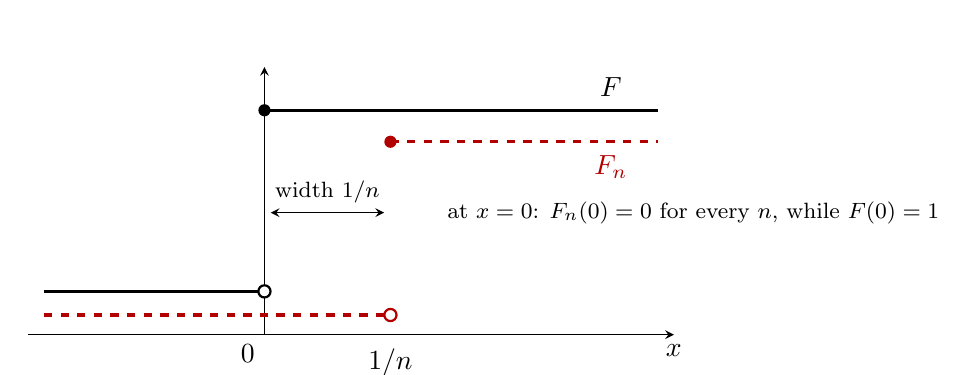
\begin{tikzpicture}[>=stealth, scale=1.0]
    % axes
    \draw[->] (-3.0,0) -- (5.2,0) node[below] {$x$};
    \draw[->] (0,0) -- (0,3.4);
    \node[below left] at (0,0) {$0$};
    % F : value 0 up to x = 0, value 1 after
    \draw[very thick] (-2.8,0.55) -- (-0.02,0.55);
    \draw[very thick] (0,2.85) -- (5.0,2.85);
    \fill (0,2.85) circle (2.2pt);
    \draw[thick,fill=white] (0,0.55) circle (2.2pt);
    \node[above] at (4.4,2.9) {$F$};
    % F_n : the same, jumping at 1/n instead
    \draw[very thick,dashed,red!70!black] (-2.8,0.25) -- (1.58,0.25);
    \draw[very thick,dashed,red!70!black] (1.6,2.45) -- (5.0,2.45);
    \fill[red!70!black] (1.6,2.45) circle (2.2pt);
    \draw[thick,fill=white,draw=red!70!black] (1.6,0.25) circle (2.2pt);
    \node[below,red!70!black] at (4.4,2.4) {$F_{n}$};
    \node[below] at (1.6,-0.05) {$1/n$};
    % the stretch on which they disagree
    \draw[<->] (0.08,1.55) -- (1.52,1.55);
    \node[above] at (0.8,1.55) {\footnotesize width $1/n$};
    \node[anchor=west,font=\footnotesize] at (2.2,1.55)
      {at $x = 0$: $F_{n}(0) = 0$ for every $n$, while $F(0) = 1$};
  \end{tikzpicture}\\[2mm]
  {\footnotesize The two fonctions en escalier take the values $0$ and $1$; they
   are drawn at slightly different heights only to keep them apart.}
\end{figure}

Le résultat suivant, dont la preuve est omise, donne deux autres façons de
caractériser la convergence en loi, and they are what make it usable: the first
replaces fonctions de répartition by fonctions test, and the second replaces them
by fonctions caractéristiques, which is the bridge back to the previous chapters
and the engine of the théorème central limite.

\begin{theorem}[Trois caractérisations de la convergence en loi]
  Soit $X_{1}, X_{2}, \dots$ une suite de variables aléatoires réelles, de
  fonctions caractéristiques respectives $\varphi_{1}, \varphi_{2}, \dots$, et
  $X$ une variable aléatoire réelle, de fonction caractéristique $\varphi$. Les
  propositions suivantes sont équivalentes :
  \begin{enumerate}
    \item La suite $X_{1}, X_{2}, \dots$ converge en loi vers $X$.
    \item Pour toute fonction \emph{continue bornée} $\phi$,
      \[
        \lim_{n \to +\infty} \expec(\phi(X_{n})) = \expec(\phi(X)) .
      \]
    \item Pour tout $t \in \reals$,
      \[
        \lim_{n \to +\infty} \varphi_{n}(t) = \varphi(t) .
      \]
  \end{enumerate}
\end{theorem}

\begin{remark}
  Both hypotheses on the fonction test in branch 2 are needed. Bounded, because
  $\expec(\phi(X_{n}))$ must exist without any integrability assumption on
  $X_{n}$ --- and the theorem is stated for arbitrary sequences, with no moments
  assumed. Continuous, because the definition tolerates failure at the
  discontinuity points of $F$, and a discontinuous fonction test can be built to
  sit exactly on one of them: taking $\phi = \indic_{(-\infty, 0]}$ in the
  deterministic example above gives $\expec(\phi(X_{n})) = 0$ for every $n$
  and $\expec(\phi(X)) = 1$.
\end{remark}

\begin{remark}
  Branch 3 is the reason the fonction caractéristique chapter comes before this
  one. It converts a question about lois --- objects with no
  arithmetic ---
  into a question about pointwise convergence of a sequence of functions on
  $\reals$, and fonctions caractéristiques of sums of independent variables
  multiply. Pointwise convergence, with no uniformity asked for anywhere, is all
  that is required. The full statement of the corresponding converse (Lévy's
  theorem, requiring the limit to be continuous at $0$) is not part of this
  course: here the limit $\varphi$ is always given in advance as the
  fonction caractéristique of an actual variable aléatoire, which is what
  branch 3 presupposes.
\end{remark}

Convergence en loi can also be read off densités when they exist, and the proof
is one application of convergence dominée followed by one application of the
theorem above.

\begin{prop}[Densités convergeant presque partout]
  Soit $X_{1}, X_{2}, \dots$ une suite de variables aléatoires réelles, de
  densités respectives $f_{1}, f_{2}, \dots$, et $X$ une variable aléatoire
  réelle, de densité $f$. Si la suite $(f_{n})_{n \geq 1}$ converge presque
  partout vers $f$, alors la suite $X_{1}, X_{2}, \dots$ converge en loi
  vers $X$.
\end{prop}

\begin{proof}
  Pour toute fonction continue bornée $\phi$, the théorème de transfert gives
  \[
    \expec(\phi(X_{n})) = \int \phi(x) f_{n}(x) \, dx
      \; \longrightarrow \; \int \phi(x) f(x) \, dx = \expec(\phi(X)) ,
  \]
  par convergence dominée: the integrands converge
  \textit{p.p.}, since $f_{n} \to f$ \textit{p.p.} and $\phi$ is fixed, and
  they are bounded in modulus by $\|\phi\|_{\infty} f_{n}$. Le résultat est
  alors une conséquence du théorème précédent --- its branch 2.
\end{proof}

\begin{remark}
  The domination needs care: the bound $\|\phi\|_{\infty} f_{n}$ moves with
  $n$, so it is not a fixed dominating function and the argument as written is a
  sketch. The repair leans on a standard result the course neither states nor
  proves (Scheffé's lemma): $f_{n} \to f$ \textit{p.p.}, all non-negative of
  integral $1$, forces $\int |f_{n} - f| \to 0$, and then
  $|\expec(\phi(X_{n})) - \expec(\phi(X))| \leq \|\phi\|_{\infty}
  \int |f_{n} - f| \to 0$, with no domination needed at all.
\end{remark}

\begin{remark}
  The implication runs one way only. Convergence en loi does not give
  convergence of densités, and the loi limite need not even have a densité: the
  two examples above converge en loi to a constant, whose loi
  is a mesure de Dirac
  with no densité at all. Convergence of densités is a genuinely stronger
  hypothesis, which is why it is stated as a sufficient condition and not as a
  characterisation.
\end{remark}

The two notions of convergence are now related. La convergence presque sûre est
plus forte que la convergence en loi :

\begin{theorem}[La convergence presque sûre implique la convergence en loi]
  Soit $X_{1}, X_{2}, \dots$ une suite de variables aléatoires réelles :
  \[
    X_{n} \cvas X \quad \Longrightarrow \quad X_{n} \cvL X .
  \]
\end{theorem}

\begin{proof}
  Pour toute fonction continue bornée $\phi$, on a par continuité (the
  stability of convergence presque sûre under a continuous map) :
  \[
    \phi(X_{n}) \cvas \phi(X) .
  \]
  La fonction $\phi$ étant bornée, the sequence $\phi(X_{n})$ is dominated by
  the constant $\|\phi\|_{\infty}$, which is integrable for the finite mesure
  $\prob$; on a donc par le théorème de convergence dominée :
  \[
    \lim_{n \to +\infty} \expec(\phi(X_{n})) = \expec(\phi(X)) .
  \]
  Le résultat découle du théorème des trois caractérisations --- this is its
  branch 2 --- so $X_{n} \cvL X$.
\end{proof}

\begin{prop}
  Si $X_{n} \cvL X$, alors $g(X_{n}) \cvL g(X)$ pour toute fonction
  continue $g$.
\end{prop}

\begin{proof}
  Pour toute fonction continue bornée $\phi$, la fonction $\phi \circ g$ est
  elle-même continue bornée --- bounded since $\phi$ is. Par le théorème des
  trois caractérisations (branch 2), applied to $X_{n} \cvL X$,
  \[
    \lim_{n \to +\infty} \expec(\phi \circ g(X_{n}))
      = \expec(\phi \circ g(X)) .
  \]
  As this holds for every bounded continuous $\phi$, l'application de ce même
  théorème, read in the other direction, implique que $g(X_{n}) \cvL g(X)$.
\end{proof}

\begin{remark}
  Both stability results are used in the same shape: prove a convergence for the
  easiest transform of the sequence --- usually a logarithm, which turns a
  product into a sum the limit theorems can reach --- then push it through the
  exponential. The examples below do this twice.
\end{remark}

\subsubsection{Liens entre les modes de convergence}
Collecting the implications, with the mode that is not part of the course drawn
dashed:

\begin{figure}[h!]
  \centering
  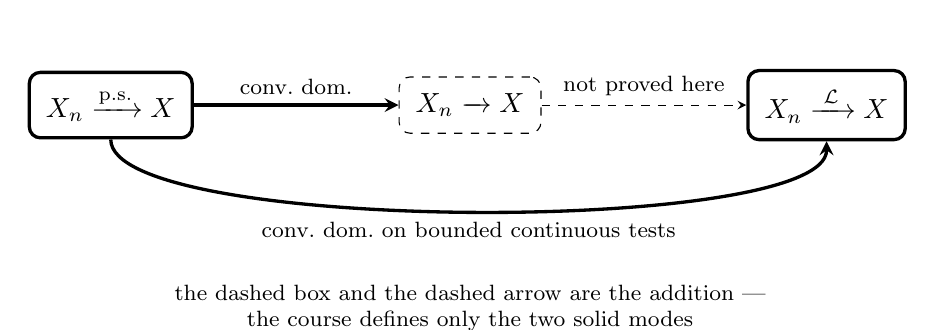
\begin{tikzpicture}[>=stealth, node distance=12mm and 26mm]
    \node[draw, very thick, rounded corners, inner sep=6pt] (as)
      {$X_{n} \cvas X$};
    \node[draw, dashed, rounded corners, inner sep=6pt, right=of as] (p)
      {$X_{n} \cvP X$};
    \node[draw, very thick, rounded corners, inner sep=6pt, right=of p] (l)
      {$X_{n} \cvL X$};
    \draw[->, very thick] (as) -- node[above,font=\footnotesize] {conv.\ dom.} (p);
    \draw[->, dashed] (p) -- node[above,font=\footnotesize] {not proved here} (l);
    \draw[->, very thick] (as.south) .. controls +(0,-1.2) and +(0,-1.2) ..
      node[below,font=\footnotesize]
      {conv.\ dom.\ on bounded continuous tests} (l.south);
    \node[below=18mm of p, align=center, font=\footnotesize]
      {the dashed box and the dashed arrow are the addition ---\\
       the course defines only the two solid modes};
  \end{tikzpicture}
\end{figure}

\begin{remark}
  None of the arrows reverses. The sliding window above converges en
  probabilité and not presque sûrement; and with $X$ of loi normale centrée
  réduite and $X_{n} = -X$ for every $n$, $X_{n} \cvL X$ holds trivially while
  $|X_{n} - X| = 2|X|$ never gets small. The one partial converse worth knowing
  belongs to the addition and is stated, not proved, here: convergence en loi
  \emph{to a constant} does imply convergence en probabilité to that constant.
\end{remark}

\subsection{Loi forte des grands nombres}
La \textbf{loi forte des grands nombres} (\textit{strong law of large numbers})
régit la limite de la moyenne empirique d'une suite de variables aléatoires
i.i.d. La seule condition est que ces variables aléatoires aient une espérance
--- no variance, no higher moment, nothing else. On parle de loi \emph{forte}
car elle implique la convergence presque sûre: a weak law would conclude only
convergence en probabilité.

\begin{theorem}[Loi forte des grands nombres]
  Pour toute suite $X_{1}, X_{2}, \dots$ de variables aléatoires réelles
  i.i.d.\ \emph{ayant une espérance},
  \[
    \frac{1}{n} \sum_{i=1}^{n} X_{i} \cvas \expec(X_{1}) .
  \]
\end{theorem}

\begin{remark}
  The hypothesis is exactly ``i.i.d.\ with an espérance'', that is,
  $\expec(|X_{1}|) < +\infty$. It is \emph{not} ``with a finite variance'': that
  stronger hypothesis belongs to the weak law and to the proof carried below,
  and importing it into the statement would weaken the theorem for no gain. The
  distinction is not academic --- the Cauchy example at the end of this
  subsection is a sequence with no espérance, and for it the theorem has
  nothing to say and the empirical mean genuinely fails to settle.
\end{remark}

\begin{proof}
  \textit{On donne une preuve partielle, dans le cas où les variables
  aléatoires ont un moment d'ordre 4.}\\
  Quitte à recentrer ces variables, on suppose que leur espérance est nulle,
  $\expec(X_{1}) = 0$, et on note
  $S_{n} = \sum_{i=1}^{n} X_{i}$.\\
  \textbf{Step 1: a bound on the moment d'ordre 4 of $S_{n}$.} Expand
  $S_{n}^{4}$ and take espérances. Indépendance makes every term containing a
  factor $X_{i}$ to the first power vanish, because $\expec(X_{1}) = 0$ and the
  factors split; what
  survives are the terms $X_{i}^{4}$, of which there are $n$, and the terms
  $X_{i}^{2}X_{j}^{2}$ with $i \neq j$, of which there are $\binom{n}{2}$ pairs
  each arising with the multinomial coefficient $\binom{4}{2}$:
  \[
    \expec(S_{n}^{4}) = n \expec(X_{1}^{4})
      + \binom{n}{2}\binom{4}{2} \expec(X_{1}^{2}X_{2}^{2}) .
  \]
  Both espérances on the right are finite and do not depend on $n$, and
  $\binom{n}{2} \leq n^{2}/2$, so $\expec(S_{n}^{4})$ grows at most like
  $n^{2}$.\\
  \textbf{Step 2: a summable series.} Soit :
  \[
    T = \sum_{n \geq 1} \left(\frac{S_{n}}{n}\right)^{4} ,
  \]
  a sum of non-negative terms, so the interchange of $\expec$ and $\sum$ is
  legitimate --- it is the Tonelli-type result for series of non-negative
  variables aléatoires from chapter 4, which needs no integrability
  hypothesis:
  \[
    \expec(T) = \sum_{n \geq 1} \frac{\expec(S_{n}^{4})}{n^{4}} .
  \]
  By step 1 the general term is $O(n^{-2})$, so the series converges and
  $\expec(T) < +\infty$.\\
  \textbf{Step 3: from an integrable sum to a vanishing term.} A non-negative
  variable aléatoire with a finite espérance is finite \textit{p.s.}: cette
  quantité étant finie, on en déduit que $T$ est \textit{p.s.} finie. A
  convergent series has a vanishing general term, so for almost every $\omega$
  the terms $(S_{n}(\omega)/n)^{4}$ tend to $0$. Ceci implique que :
  \[
    \frac{S_{n}}{n} \cvas 0 ,
  \]
  which is the claim after undoing the recentring.
\end{proof}

\begin{remark}
  The technique of step 3 is the one to carry away, and it is more general than
  the theorem: to prove that a sequence of variables aléatoires converges
  presque sûrement to $0$, it is enough to show that the \emph{series} of some
  positive power of it has finite espérance. The fourth power is used rather than the
  second because the second is not summable --- $\expec(S_{n}^{2})/n^{2} = 1/n$
  for unit-variance variables, and $\sum 1/n$ diverges. Going up to the fourth
  power buys the extra factor of $n$ at the cost of a moment hypothesis that the
  full theorem does not need.
\end{remark}

\begin{example}[Empirical frequency of a Bernoulli trial]
  Soit $X_{1}, X_{2}, \dots$ une suite de variables aléatoires i.i.d.\ suivant
  une loi de Bernoulli $\mathcal{B}(p)$ de paramètre
  $p \in [0,1]$. Alors :
  \[
    \frac{1}{n} \sum_{i=1}^{n} X_{i} \cvas p .
  \]
  The empirical frequency of an événement converges presque sûrement to its
  probability, which is the statement that makes the frequentist reading of
  $\prob$ a theorem rather than a definition.
\end{example}

\begin{example}[Empirical mean of a centred normal sample]
  Soit $X_{1}, X_{2}, \dots$ une suite de variables aléatoires i.i.d.\ de loi
  normale centrée réduite $\mathcal{N}(0,1)$. Alors :
  \[
    \frac{1}{n} \sum_{i=1}^{n} X_{i} \cvas 0 .
  \]
  Worth contrasting with the exact loi: $\frac{1}{n}S_{n} \sim
  \mathcal{N}(0, 1/n)$ for every $n$, the Gaussian collapsing onto a point from
  the earlier example. The loi forte says more than that collapse --- it says
  the convergence holds $\omega$ by $\omega$, not merely en loi.
\end{example}

\begin{example}[A loi with no espérance: Cauchy]
  Soit $X_{1}, X_{2}, \dots$ une suite de variables aléatoires i.i.d.\ de loi de
  Cauchy. Cette loi n'ayant pas d'espérance, la loi des grands nombres ne
  s'applique pas, and the empirical mean does not converge --- in fact
  $\frac{1}{n}S_{n}$ has the same loi de Cauchy for every $n$, so it does not
  settle anywhere. On a par contre --- the positive and negative parts both
  blow up :
  \[
    \frac{1}{n} \sum_{i=1}^{n} X_{i}^{+} \cvas +\infty
    \qquad \text{and} \qquad
    \frac{1}{n} \sum_{i=1}^{n} X_{i}^{-} \cvas +\infty ,
  \]
  two limits stated here without proof. The theorem above does not
  supply them: $X_{1}^{+}$ and $X_{1}^{-}$ have infinite espérance, so they
  fall outside its hypothesis. What they need is the extension of the loi forte
  to non-negative variables of infinite espérance, obtained by truncation,
  which this course does not state. The empirical mean is then the difference of
  two sequences both going to $+\infty$, and the indeterminacy is real, not an
  artefact of the proof.
\end{example}

\begin{example}[Three means of a Beta sample]
  Soit $X_{1}, \dots, X_{n}$ des variables aléatoires i.i.d.\ de loi
  $\mathcal{B}(2,1)$, whose densité is $2x$ on $[0,1]$. Each of the three
  classical means has an almost-sure limit, and each is the loi forte applied to
  a different transform of the sample.\\
  The arithmetic mean converges to $\expec(X_{1}) = \int_{0}^{1} 2x^{2}dx =
  2/3$.\\
  The geometric mean is handled by taking a logarithm, which turns it into an
  arithmetic mean:
  \[
    \ln\left(\prod_{i=1}^{n} X_{i}\right)^{1/n}
      = \frac{1}{n}\sum_{i=1}^{n} \ln X_{i} \cvas \expec(\ln X_{1})
      = \int_{0}^{1} 2x \ln x \, dx = -\frac{1}{2} ,
  \]
  and pushing through the exponential, which is continuous, gives the geometric
  mean converging \textit{p.s.} to $e^{-1/2}$.\\
  The harmonic mean is the reciprocal of the arithmetic mean of the reciprocals:
  $\frac{1}{n}\sum 1/X_{i} \cvas \expec(1/X_{1}) = \int_{0}^{1} 2 \, dx = 2$, and
  the reciprocal being continuous away from $0$, the harmonic mean converges
  \textit{p.s.} to $1/2$.\\
  The three limits satisfy $1/2 < e^{-1/2} \approx 0.607 < 2/3$, the usual
  ordering of means --- a cheap check on the arithmetic.
\end{example}

\begin{example}[The digits of a uniform variable]
  Soit $U$ une variable aléatoire uniforme sur $[0,1]$, and write its binary
  expansion $U = \sum_{k \geq 1} b_{k} 2^{-k}$. The digits
  $b_{1}, b_{2}, \dots$ are i.i.d.\ of loi $\mathcal{B}(1/2)$ --- each is
  determined by which half of a dyadic interval $U$ falls in, and the halves are
  chosen independently by uniformity. By the loi forte, la fraction de 1 des $n$
  premiers bits de sa décomposition binaire tend presque sûrement vers un
  demi :
  \[
    \frac{1}{n} \sum_{k=1}^{n} b_{k} \cvas \frac{1}{2} .
  \]
  The exceptional set is not empty: it contains the dyadic rationals, whose
  expansions are eventually constant. It is far larger than that --- every $u$
  whose digit frequency is some other value lies in it too, and those form an
  uncountable family --- so its negligibility comes from the loi forte itself
  and not from counting. That is exactly the licence the word \textit{presque}
  gives.
\end{example}

\begin{example}[A random number of terms]
  Soit $X_{1}, X_{2}, \dots$ une suite de variables aléatoires i.i.d.\ de loi de
  Bernoulli $\mathcal{B}(p)$ de paramètre $p > 0$, with partial sums $S_{n}$. On
  note $Y_{1}, Y_{2}, \dots$ une suite de variables aléatoires i.i.d.\ de loi
  Poisson $\mathcal{P}(\lambda)$, independent of the first sequence. Then
  \[
    \frac{1}{n} \sum_{k=1}^{S_{n}} Y_{k} \cvas p\lambda .
  \]
  Factor the quantity as
  $\frac{S_{n}}{n} \cdot \frac{1}{S_{n}}\sum_{k \leq S_{n}} Y_{k}$. The first
  factor tends \textit{p.s.} to $p$ by the loi forte. For the second, $p > 0$
  forces $S_{n} \to +\infty$ \textit{p.s.}, so it is the empirical mean of the
  $Y$ sequence along indices tending to infinity and tends \textit{p.s.} to
  $\expec(Y_{1}) = \lambda$. The two almost-sure événements intersect in one of
  probability $1$, on which the limits multiply.
\end{example}

\begin{example}[Équirépartition asymptotique]
  Soit $X_{1}, X_{2}, \dots$ une suite de variables aléatoires i.i.d.\ sur
  $\{1, \dots, K\}$ --- a finite alphabet --- et
  $p(k_{1}, \dots, k_{n}) = \prob(X_{1} = k_{1}, \dots, X_{n} = k_{n})$,
  the probability of an observed word. Indépendance factorises it, so taking
  a logarithm turns it into a sum the loi forte reaches:
  \[
    -\frac{1}{n} \ln p(X_{1}, \dots, X_{n})
      = -\frac{1}{n}\sum_{i=1}^{n} \ln p_{X_{i}}
      \cvas -\expec\big(\ln p_{X_{1}}\big)
      = -\sum_{k=1}^{K} p_{k} \ln p_{k} ,
  \]
  where $p_{k} = \prob(X_{1} = k)$. Il s'agit de
  l'entropie de la loi de $X_{1}$ : $H = -\sum_{k} p_{k}\ln p_{k}$. Par continuité de la fonction exponentielle, on obtient
  \[
    \sqrt[n]{p(X_{1}, \dots, X_{n})} \cvas e^{-H} :
  \]
  almost every long word has probability close to $e^{-nH}$, so the $K^{n}$
  possible words split into roughly $e^{nH}$ words of nearly equal probability
  and a remainder of négligeable total probability. This is the loi forte doing
  the work that information theory calls the \textbf{équirépartition
  asymptotique} (\textit{asymptotic equipartition property}).
\end{example}

\begin{example}[A limiting geometric mean]
  Let $U_{1}, U_{2}, \dots$ be i.i.d.\ uniform on $(0,1)$. First,
  $-\ln U_{1}$ follows the loi exponentielle $\mathcal{E}(1)$: for every
  mesurable $\phi \geq 0$, the changement de variable $v = -\ln u$ gives
  \[
    \expec(\phi(-\ln U_{1})) = \int_{0}^{1} \phi(-\ln u)\, du
      = \int_{0}^{+\infty} \phi(v) e^{-v} dv ,
  \]
  which identifies the loi by the théorème de transfert. Hence
  $\expec(\ln U_{1}) = -1$. Writing $G_{n} = \sqrt[n]{U_{1}U_{2}\cdots U_{n}}$
  and taking a logarithm,
  \[
    \ln G_{n} = \frac{1}{n}\sum_{i=1}^{n} \ln U_{i} \cvas -1 ,
  \]
  by the loi forte, and the exponential being continuous,
  \[
    G_{n} \cvas \frac{1}{e} .
  \]
  The geometric mean of uniform variables does not converge to the arithmetic
  mean $1/2$ but to $1/e \approx 0.368$, which is smaller, as it must be. The
  same sequence reappears in the next subsection, where the théorème central
  limite describes its fluctuations.
\end{example}

\subsection{Théorème central limite}
The loi forte says where the empirical mean goes. Le \textbf{théorème central
limite} (\textit{central limit theorem}) s'intéresse à la loi des écarts à la
moyenne empirique, toujours pour une suite de variables aléatoires i.i.d.: it
says how the mean gets there, describing the deviation from the limit once that
deviation is magnified by the right factor. On suppose que ces variables ont un
moment d'ordre $2$ (donc d'espérance et de variance finies) --- a hypothesis
one notch stronger than the loi forte's --- and the conclusion is one notch
weaker, convergence en loi rather than convergence presque sûre. That trade is
the whole content of the theorem.

\begin{theorem}[Théorème central limite]
  Pour toute suite $X_{1}, X_{2}, \dots$ de variables aléatoires réelles
  i.i.d.\ d'espérance finie $\mu$ et de variance finie $\sigma^{2}$,
  \[
    \sqrt{n}\left(\frac{1}{n}\sum_{i=1}^{n} X_{i} - \mu\right)
      \cvL \mathcal{N}(0, \sigma^{2}) .
  \]
\end{theorem}

\begin{remark}
  The $\sqrt{n}$ is not adjustable. The quantity in brackets tends to $0$
  \textit{p.s.} by the loi forte, so any factor growing more slowly than
  $\sqrt{n}$ would give the constant $0$ in the limit and any factor growing
  faster would give no limit at all; $\sqrt{n}$ is the unique scale at which the
  deviation has a loi limite non dégénérée, and it is dictated by the variance
  of the mean being $\sigma^{2}/n$. Note also what the loi limite does
  \emph{not} depend on: the loi of $X_{1}$ enters only through
  $\sigma^{2}$.
  That is the universality the theorem is famous for.
\end{remark}

\begin{proof}
  \textbf{Reductions.} Quitte à recentrer les variables aléatoires, on peut
  supposer que leur espérance est nulle, $\mu = 0$. Si leur variance est nulle,
  $\sigma^{2} = 0$, le résultat est évident: the variables are \textit{p.s.}
  constant and the left-hand side is \textit{p.s.} zero; sinon, quitte à les
  renormaliser (by $\sigma$), on peut supposer que leur variance est égale à 1,
  $\sigma^{2} = 1$. On note encore
  $S_{n} = \sum_{i=1}^{n} X_{i}$. On s'intéresse à la loi limite de la variable
  aléatoire $S_{n}/\sqrt{n}$.\\
  \textbf{Step 1: factorise the fonction caractéristique.} The variables being
  indépendantes et identiquement distribuées, the fonction caractéristique of
  the sum is the product of the fonctions caractéristiques, and scaling the
  argument handles the $\sqrt{n}$:
  \[
    \forall t \in \reals, \qquad
    \varphi_{S_{n}/\sqrt{n}}(t) = \varphi_{S_{n}}\!\left(\frac{t}{\sqrt{n}}\right)
      = \varphi_{X_{1}}\!\left(\frac{t}{\sqrt{n}}\right)^{\! n} .
  \]
  \textbf{Step 2: expand at the origin.} $X_{1}$ has a moment d'ordre $2$, so
  its fonction caractéristique is twice differentiable at $0$ and the expansion
  from the fonction caractéristique chapter applies. Comme cette variable est supposée
  d'espérance nulle et de variance 1 (suite à l'étape initiale de recentrage et
  normalisation), that is $\expec(X_{1}) = 0$ and
  $\Var(X_{1}) = 1$, the first-order term vanishes and
  \[
    \varphi_{X_{1}}(t) = 1 - \frac{t^{2}}{2} + o(t^{2}) ,
    \qquad \text{so} \qquad
    \varphi_{X_{1}}\!\left(\frac{t}{\sqrt{n}}\right)
      = 1 - \frac{t^{2}}{2n} + o\!\left(\frac{t^{2}}{n}\right) .
  \]
  \textbf{Step 3: compare the $n$-th powers.} Fix $t$. Pour $n$ assez grand, on
  a $|1 - t^{2}/(2n)| \leq 1$ et donc, by the elementary bound
  $|a^{n} - b^{n}| \leq n|a-b|$ for complex $a, b$ of modulus at most $1$ :
  \[
    \left| \varphi_{X_{1}}\!\left(\frac{t}{\sqrt{n}}\right)^{\! n}
      - \left(1 - \frac{t^{2}}{2n}\right)^{\! n} \right|
    \leq n \left| \varphi_{X_{1}}\!\left(\frac{t}{\sqrt{n}}\right)
      - \left(1 - \frac{t^{2}}{2n}\right) \right|
    = n \cdot o\!\left(\frac{t^{2}}{n}\right)
    \; \longrightarrow \; 0 .
  \]
  \textbf{Step 4: identify the limit.} Since
  $(1 - t^{2}/(2n))^{n} \to e^{-t^{2}/2}$, on en déduit que :
  \[
    \lim_{n \to +\infty} \varphi_{S_{n}/\sqrt{n}}(t)
      = \lim_{n \to +\infty}
        \varphi_{X_{1}}\!\left(\frac{t}{\sqrt{n}}\right)^{\! n}
      = e^{-t^{2}/2} ,
  \]
  qui est la fonction caractéristique d'une loi normale centrée réduite, as
  computed in the fonction caractéristique chapter. Par le théorème des trois
  caractérisations (branch 3),
  \[
    \frac{S_{n}}{\sqrt{n}} \cvL \mathcal{N}(0,1) .
  \]
  Undoing the two reductions --- multiplying back by $\sigma$ and restoring
  $\mu$ --- gives the statement.
\end{proof}

\begin{remark}
  Every hypothesis is visible in exactly one step. Being identiquement
  distribuées is what makes step 1 a single fonction caractéristique raised to
  a power rather than a product of $n$ different ones. Indépendance is what
  makes it a product at all.
  The moment d'ordre $2$ is what makes step 2 legitimate, and it is the only
  place any moment is used --- there is no moment d'ordre 3 anywhere in the
  proof, and none is needed. Step 3 is a purely analytic estimate with no
  probability in it. The convergence obtained is pointwise in $t$, which is
  precisely what branch 3 asks for.
\end{remark}

\begin{remark}
  The specialisation $S_{n}/\sqrt{n} \cvL \mathcal{N}(0,1)$, obtained in step 4
  for variables centrées of unit variance, is the form actually used in
  computations: it says that a sum of $n$ i.i.d.\ variables centrées is of order
  $\sqrt{n}$, with Gaussian fluctuations. For variables of variance
  $\sigma^{2}$ the same statement reads
  $S_{n}/\sqrt{n} \cvL \mathcal{N}(0, \sigma^{2})$, and for variables that are
  not centrées
  $(S_{n} - n\mu)/\sqrt{n} \cvL \mathcal{N}(0, \sigma^{2})$, which is the
  theorem multiplied out.
\end{remark}

The figure shows the convergence taking place for the least Gaussian-looking
starting point available: the loi uniforme on $[0,1]$. Each panel plots the
exact densité of the standardised sum of $n$ such variables against the
densité of the loi normale centrée réduite. At $n = 1$ the two could hardly look less alike; at $n = 2$ the
sum is triangular; by $n = 5$ the shape is already close; at $n = 30$ the two
curves are indistinguishable at this scale.

\begin{figure}[h!]
  \centering
  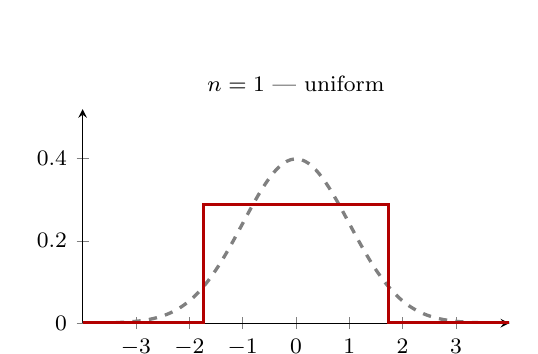
\begin{tikzpicture}
    \begin{axis}[
      title={$n = 1$ --- uniform},
      width=7.0cm, height=4.3cm,
      axis lines=left,
      xmin=-4, xmax=4, ymin=0, ymax=0.52,
      xtick={-3,-2,-1,0,1,2,3}, ytick={0,0.2,0.4},
      tick label style={font=\footnotesize},
      title style={font=\footnotesize, yshift=-3pt},
      every axis plot/.append style={very thick},
    ]
      \addplot[gray, dashed, domain=-4:4, samples=120]
        {0.3989423*exp(-x^2/2)};
      \addplot[red!70!black] coordinates
        {(-4,0) (-1.7321,0) (-1.7321,0.28868) (1.7321,0.28868)
         (1.7321,0) (4,0)};
    \end{axis}
  \end{tikzpicture}
  \hfill
  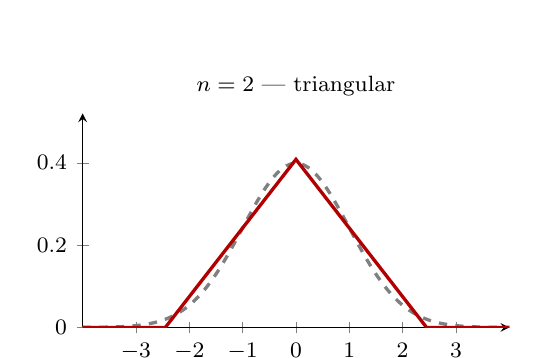
\begin{tikzpicture}
    \begin{axis}[
      title={$n = 2$ --- triangular},
      width=7.0cm, height=4.3cm,
      axis lines=left,
      xmin=-4, xmax=4, ymin=0, ymax=0.52,
      xtick={-3,-2,-1,0,1,2,3}, ytick={0,0.2,0.4},
      tick label style={font=\footnotesize},
      title style={font=\footnotesize, yshift=-3pt},
      every axis plot/.append style={very thick},
    ]
      \addplot[gray, dashed, domain=-4:4, samples=120]
        {0.3989423*exp(-x^2/2)};
      \addplot[red!70!black] coordinates
        {(-4,0) (-2.4495,0) (0,0.40825) (2.4495,0) (4,0)};
    \end{axis}
  \end{tikzpicture}

  \vspace{4mm}

  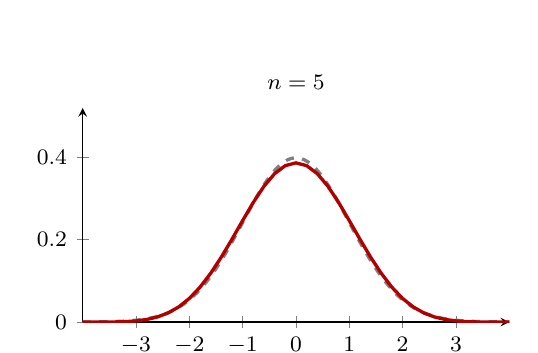
\begin{tikzpicture}
    \begin{axis}[
      title={$n = 5$},
      width=7.0cm, height=4.3cm,
      axis lines=left,
      xmin=-4, xmax=4, ymin=0, ymax=0.52,
      xtick={-3,-2,-1,0,1,2,3}, ytick={0,0.2,0.4},
      tick label style={font=\footnotesize},
      title style={font=\footnotesize, yshift=-3pt},
      every axis plot/.append style={very thick},
    ]
      \addplot[gray, dashed, domain=-4:4, samples=120]
        {0.3989423*exp(-x^2/2)};
      \addplot[red!70!black] coordinates {
        (-4.0,0.0) (-3.8,0.0) (-3.6,0.00003) (-3.4,0.00023) (-3.2,0.00096) (-3.0,0.00271)
        (-2.8,0.00619) (-2.6,0.01226) (-2.4,0.02198) (-2.2,0.03657) (-2.0,0.05721) (-1.8,0.08447)
        (-1.6,0.11823) (-1.4,0.15764) (-1.2,0.20113) (-1.0,0.24642) (-0.8,0.29052) (-0.6,0.32974)
        (-0.4,0.36045) (-0.2,0.37995) (0.0,0.38663) (0.2,0.37995) (0.4,0.36045) (0.6,0.32974)
        (0.8,0.29052) (1.0,0.24642) (1.2,0.20113) (1.4,0.15764) (1.6,0.11823) (1.8,0.08447)
        (2.0,0.05721) (2.2,0.03657) (2.4,0.02198) (2.6,0.01226) (2.8,0.00619) (3.0,0.00271)
        (3.2,0.00096) (3.4,0.00023) (3.6,0.00003) (3.8,0.0) (4.0,0.0)};
    \end{axis}
  \end{tikzpicture}
  \hfill
  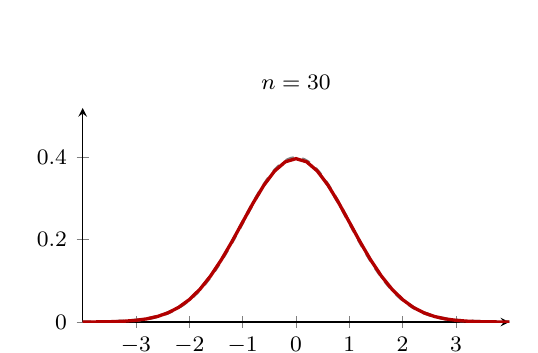
\begin{tikzpicture}
    \begin{axis}[
      title={$n = 30$},
      width=7.0cm, height=4.3cm,
      axis lines=left,
      xmin=-4, xmax=4, ymin=0, ymax=0.52,
      xtick={-3,-2,-1,0,1,2,3}, ytick={0,0.2,0.4},
      tick label style={font=\footnotesize},
      title style={font=\footnotesize, yshift=-3pt},
      every axis plot/.append style={very thick},
    ]
      \addplot[gray, dashed, domain=-4:4, samples=120]
        {0.3989423*exp(-x^2/2)};
      \addplot[red!70!black] coordinates {
        (-4.0,0.0001) (-3.8,0.00023) (-3.6,0.00052) (-3.4,0.00109) (-3.2,0.00219) (-3.0,0.0042)
        (-2.8,0.00768) (-2.6,0.01339) (-2.4,0.02233) (-2.2,0.03563) (-2.0,0.05445) (-1.8,0.07975)
        (-1.6,0.11202) (-1.4,0.15097) (-1.2,0.19534) (-1.0,0.24278) (-0.8,0.28989) (-0.6,0.33267)
        (-0.4,0.36699) (-0.2,0.38924) (0.0,0.39694) (0.2,0.38924) (0.4,0.36699) (0.6,0.33267)
        (0.8,0.28989) (1.0,0.24278) (1.2,0.19534) (1.4,0.15097) (1.6,0.11202) (1.8,0.07975)
        (2.0,0.05445) (2.2,0.03563) (2.4,0.02233) (2.6,0.01339) (2.8,0.00768) (3.0,0.0042)
        (3.2,0.00219) (3.4,0.00109) (3.6,0.00052) (3.8,0.00023) (4.0,0.0001)};
    \end{axis}
  \end{tikzpicture}
\end{figure}

\begin{example}[Fluctuations of a Bernoulli frequency]
  Soit $X_{1}, X_{2}, \dots$ une suite de variables aléatoires i.i.d.\ suivant
  une loi de Bernoulli $\mathcal{B}(p)$ de paramètre
  $p \in [0,1]$. The variance is $p(1-p)$, so
  \[
    \sqrt{n}\left(\frac{1}{n}\sum_{i=1}^{n} X_{i} - p\right)
      \cvL \mathcal{N}(0, p(1-p)) .
  \]
  Autrement dit, pour $n$ assez grand, la loi de l'écart de la moyenne
  empirique à la valeur limite $p$ est proche d'une loi normale centrée et de
  variance $p(1-p)/n$.
  This is the statement behind every confidence interval for a proportion.
\end{example}

\begin{example}[A loi du $\chi^{2}$ is asymptotically normal]
  La loi du $\chi^{2}$ à $n$ degrés de liberté is by definition the loi of
  $Z_{1}^{2} + \cdots + Z_{n}^{2}$ with $Z_{1}, \dots, Z_{n}$ i.i.d.\
  $\mathcal{N}(0,1)$. The summands are i.i.d.; comme
  $\expec(Z_{1}^{2}) = 1$ et
  $\Var(Z_{1}^{2}) = \expec(Z_{1}^{4}) - 1 = 3 - 1 = 2$, both finite, the
  théorème central limite applies to them. Formellement,
  \[
    \frac{1}{\sqrt{n}}\left(\sum_{i=1}^{n} Z_{i}^{2} - n\right)
      \cvL \mathcal{N}(0,2) .
  \]
  La loi $\chi^{2}(n)$ est donc proche de $\mathcal{N}(n, 2n)$, pourvu que $n$
  soit assez grand. The moment $\expec(Z_{1}^{4}) = 3$ is the moment d'ordre 4
  of the loi normale centrée réduite, read off the fourth-order expansion of
  $e^{-t^{2}/2}$ in the fonction caractéristique chapter.
\end{example}

\begin{example}[A Poisson sum cut at its mean]
  For $a, n > 0$ set $F(a,n) = \sum_{k=0}^{\lfloor an \rfloor} n^{k}/k!$. Since
  a sum of $n$ i.i.d.\ $\mathcal{P}(1)$ variables follows $\mathcal{P}(n)$ ---
  which the fonction génératrice settles in one line, $G_{Y}(s) = e^{n(s-1)} =
  (e^{s-1})^{n}$ --- one may write $e^{-n}F(a,n) = \prob(Y \leq an)$ with
  $Y \sim \mathcal{P}(n)$, that is, $Y = X_{1} + \cdots + X_{n}$ for i.i.d.\
  $\mathcal{P}(1)$ variables.\\
  For $a \in (0,1)$, the loi forte gives
  $\frac{1}{n}(X_{1} + \cdots + X_{n}) \cvas 1$, hence convergence en loi to
  the constant $1$, whose fonction de répartition is continuous at
  $a < 1$; therefore $e^{-n}F(a,n) = \prob(\frac{1}{n}\sum X_{i} \leq a) \to 0$.\\
  At the critical value $a = 1$ the loi forte says nothing, since $1$ is the
  discontinuity point of the limit, and the théorème central limite takes over:
  $\sqrt{n}(\frac{1}{n}\sum X_{i} - 1) \cvL \mathcal{N}(0,1)$ because
  $\mathcal{P}(1)$ has espérance and variance both equal to $1$, and $0$ is a
  continuity point of the fonction de répartition of the loi normale, so
  \[
    e^{-n}F(1,n) = \prob\!\left(\sqrt{n}\left(\tfrac{1}{n}\textstyle\sum_{i} X_{i}
      - 1\right) \leq 0\right) \; \longrightarrow \; \frac{1}{2} .
  \]
  The example is the clearest illustration of the division of labour between the
  two theorems: away from the mean the loi forte decides, and exactly at the
  mean only the théorème central limite can.
\end{example}

\begin{example}[Fluctuations of the limiting geometric mean]
  Continuing the uniform example of the previous subsection, with
  $G_{n} = \sqrt[n]{U_{1}\cdots U_{n}}$ and $\expec(\ln U_{1}) = -1$. Set
  $Z_{n} = (c\,G_{n})^{\sqrt{n}}$ and take a logarithm:
  \[
    \ln Z_{n} = \sqrt{n}\left(\ln c + \frac{1}{n}\sum_{i=1}^{n} \ln U_{i}\right) .
  \]
  This is the théorème central limite's expression provided $\ln c$ cancels the
  espérance, that is $\ln c = -\expec(\ln U_{1}) = 1$, so $c = e$. Since
  $-\ln U_{1} \sim \mathcal{E}(1)$ has variance $1$,
  \[
    \ln Z_{n} \cvL \mathcal{N}(0,1) ,
  \]
  and the exponential being continuous, $Z_{n} \cvL Z = e^{X}$ with
  $X \sim \mathcal{N}(0,1)$. The densité of $Z$ follows from the théorème de
  transfert and the changement de variable $z = e^{x}$. Pour toute fonction
  mesurable $\phi \geq 0$,
  \[
    \expec(\phi(Z)) = \int_{\reals} \phi(e^{x})
      \frac{1}{\sqrt{2\pi}} e^{-x^{2}/2} dx
    = \int_{0}^{+\infty} \phi(z) \frac{1}{\sqrt{2\pi}\,z}
      e^{-(\ln z)^{2}/2} \, dz ,
  \]
  la densité est donc :
  \[
    f_{Z}(z) = \frac{1}{\sqrt{2\pi}\,z} e^{-(\ln z)^{2}/2}
      \indic_{\reals_{+}}(z) ,
  \]
  c'est une \textbf{loi log-normale} (\textit{log-normal distribution}). Between
  them, this example and the one it continues use both stability results of the
  first two subsections, in the same shape --- the presque sûre one there, the
  one for convergence en loi here:
  the logarithm turns the product into a sum, the limit theorem acts on the sum,
  the exponential carries the conclusion back.
\end{example}

\begin{example}[Excess of ones over zeros in a binary expansion]
  Soit $U$ une variable aléatoire uniforme sur $[0,1]$. On note $X_{n}$ et
  $Y_{n}$ les nombres de 0 et de 1 parmi les $n$ premiers bits de sa
  décomposition binaire. With
  $b_{1}, b_{2}, \dots$ i.i.d.\ of loi $\mathcal{B}(1/2)$ as before,
  $Y_{n} = \sum_{k \leq n} b_{k}$ and $X_{n} = n - Y_{n}$, so
  \[
    X_{n} - Y_{n} = \sum_{k=1}^{n} (1 - 2b_{k}) .
  \]
  The summands $1 - 2b_{k}$ are i.i.d., take the values $\pm 1$ with probability
  $1/2$ each, and so have espérance $0$ and variance $1$. The specialised form
  of the théorème central limite applies directly:
  \[
    \frac{X_{n} - Y_{n}}{\sqrt{n}} \cvL \mathcal{N}(0,1) .
  \]
  The loi forte already said that the excess is $o(n)$; the théorème central
  limite says it is of order exactly $\sqrt{n}$, with Gaussian fluctuations.
\end{example}

\begin{example}[A rate the théorème central limite does not supply]
  The théorème central limite is a statement about a limit and gives no bound at
  any fixed $n$. When a bound is wanted --- an \textbf{inégalité de déviation}
  (\textit{deviation inequality}) --- the route is the exponential moment, and
  it is worth carrying because the technique reappears whenever a rate is asked
  for.\\
  Let $Y_{1}, Y_{2}, \dots$ be i.i.d.\ on $\{-1,+1\}$ with
  $\prob(Y_{1} = 1) = 1/2$, and $S_{n} = Y_{1} + \cdots + Y_{n}$. Fix $a > 0$.
  \begin{enumerate}
    \item \emph{Exponentiate, then apply Markov.} For every $x > 0$ the map
      $s \mapsto e^{xs}$ is increasing, so $\{S_{n} > a\} = \{e^{xS_{n}} >
      e^{xa}\}$, and the inégalité de Markov applied to the non-negative
      variable $e^{xS_{n}}$ gives $\prob(S_{n} > a) \leq e^{-ax}\expec(e^{xS_{n}})$.
    \item \emph{Compute the exponential moment.} The variables being
      indépendantes et identiquement distribuées,
      $\expec(e^{xS_{n}}) = \expec(e^{xY_{1}})^{n} = \cosh(x)^{n}$, since
      $\expec(e^{xY_{1}}) = \frac{1}{2}(e^{x} + e^{-x})$.
    \item \emph{Bound it.} Studying the sign of $x \mapsto x^{2}/2 -
      \ln\cosh(x)$, whose derivative $x - \tanh(x)$ is non-negative on
      $\reals_{+}$ and which vanishes at $0$, gives $\cosh(x) \leq e^{x^{2}/2}$,
      hence $\expec(e^{xS_{n}}) \leq e^{nx^{2}/2}$ for $x > 0$.
    \item \emph{Optimise.} The bound is now $e^{-ax + nx^{2}/2}$; minimising the
      exponent over $x > 0$ gives $x = a/n$ and
      $\prob(S_{n} > a) \leq e^{-a^{2}/(2n)}$.
    \item \emph{Symmetrise.} The loi of $S_{n}$ is symétrique, so the borne de
      l'union gives $\prob(|S_{n}| > a) \leq 2e^{-a^{2}/(2n)}$.
  \end{enumerate}
  Two things to notice. The bound holds at every $n$, not asymptotically, which
  is what the limit theorems never give. And taking $a = \varepsilon n$ gives
  $\prob(|S_{n}/n| > \varepsilon) \leq 2e^{-\varepsilon^{2}n/2}$, an exponential
  rate for a convergence that the loi forte, read through the implication of
  the first subsection, gives without any rate at all.
\end{example}

\subsection{Cas des vecteurs aléatoires}
La loi des grands nombres et le théorème central limite s'étendent sans
difficulté au cas vectoriel. The empirical mean is taken coordinate by
coordinate, the espérance becomes a vector, and the variance becomes a matrice
de covariance $\Gamma$.

\begin{theorem}[Loi forte des grands nombres -- cas vectoriel]
  Pour toute suite $X_{1}, X_{2}, \dots$ de vecteurs aléatoires réels
  i.i.d.\ \emph{ayant une espérance},
  \[
    \frac{1}{n} \sum_{i=1}^{n} X_{i} \cvas \expec(X_{1}) .
  \]
\end{theorem}

\begin{theorem}[Théorème central limite -- cas vectoriel]
  Pour toute suite $X_{1}, X_{2}, \dots$ de vecteurs aléatoires réels i.i.d.\
  d'espérance finie $\mu$ et de matrice de covariance finie $\Gamma$,
  \[
    \sqrt{n}\left(\frac{1}{n}\sum_{i=1}^{n} X_{i} - \mu\right)
      \cvL \mathcal{N}(0, \Gamma) .
  \]
\end{theorem}

\begin{remark}
  The loi forte in the vector case is the scalar one applied to each
  coordinate, together with the fact that a finite intersection of événements
  of probability $1$ has probability $1$ --- which is why it costs nothing. The
  théorème central limite in the vector case is genuinely more than its
  coordinates: convergence en loi of each coordinate does not give convergence
  en loi of the vector, since the loi jointe is not determined by the lois
  marginales. What repairs this is the fonction caractéristique of a vecteur
  aléatoire, which does determine the loi jointe, together with the vector form
  of branch 3: pointwise convergence of fonctions caractéristiques on
  $\reals^{d}$, $d$ being the dimension of the vectors, gives convergence en
  loi. That vector form is the missing ingredient and is stated, not proved,
  here --- the characterisation theorem above is for variables aléatoires
  réelles, and this course states the vector case without supplying it. The
  matrice de covariance
  $\Gamma$ carries the dependence between coordinates that the lois marginales
  lose.
\end{remark}

\begin{remark}
  ``Matrice de covariance finie'' means every entry finite, that is, a moment
  d'ordre $2$ for every coordinate. No invertibility of $\Gamma$ is required
  anywhere: a $\Gamma$ that is dégénérée gives a vecteur gaussien supported on
  a proper subspace, which is a perfectly good limit en loi even though it has
  no densité on $\reals^{d}$.
\end{remark}

\begin{example}[Uniform points on the unit disc]
  Soit $X_{1}, X_{2}, \dots$ une suite de vecteurs aléatoires réels i.i.d.\ (in
  $\reals^{2}$) de loi uniforme sur le disque unité. Their espérance is $0$ by
  symmetry, and leur matrice de covariance est $I/4$, où $I$ désigne la matrice
  identité en dimension $2$: writing
  $X_{1} = (X, Y)$ for the two coordinates of one point, the off-diagonal entry
  $\expec(XY)$ vanishes by symmetry, and in polar coordinates the diagonal entry
  is
  \[
    \expec(X^{2}) = \frac{1}{\pi}\int_{0}^{2\pi}\!\!\int_{0}^{1}
      r^{2}\cos^{2}\theta \cdot r \, dr \, d\theta
    = \frac{1}{\pi} \cdot \frac{1}{4} \cdot \pi = \frac{1}{4} .
  \]
  Alors, by the théorème central limite in the vector case,
  \[
    \sqrt{n}\left(\frac{1}{n}\sum_{i=1}^{n} X_{i}\right)
      \cvL \mathcal{N}\!\left(0, \frac{I}{4}\right) .
  \]
  The limit is a rescaled vecteur gaussien centré réduit, so its level sets are
  circles: the isotropy of the disc survives into the limit.
\end{example}

\begin{example}[The barycentre of random points]
  Soit $G_{n}$ le barycentre de $n$ points aléatoires indépendants de même loi
  uniforme sur le disque unité. Then $G_{n} = \frac{1}{n}\sum_{i \leq n} X_{i}$
  is exactly the empirical mean of the previous example, so $G_{n} \cvas 0$ by
  the loi forte in the vector case, and
  \[
    \sqrt{n}\, G_{n} \cvL \mathcal{N}\!\left(0, \frac{I}{4}\right) .
  \]
  The barycentre of many random points is near the centre, at distance of order
  $1/\sqrt{n}$, and its fluctuation is isotropic Gaussian.
\end{example}

\begin{example}[Order statistics of two uniform variables]
  Soient $U, V$ deux variables aléatoires indépendantes de loi uniforme sur
  $[0,1]$. On note le vecteur
  $Z = (X, Y)$ avec $X = \min(U,V)$ et $Y = \max(U,V)$, et
  $Z_{1}, Z_{2}, \dots$ une suite de vecteurs aléatoires i.i.d.\ de même loi
  que $Z$.\\
  \emph{The loi of $Z$.} The pair $(U,V)$ has densité $\indic_{[0,1]^{2}}$, and
  $(X,Y)$ is obtained by folding the square along its diagonal --- the two
  points $(u,v)$ and $(v,u)$ give the same $(x,y)$ --- so
  \[
    f_{Z}(x,y) = 2 \, \indic_{\{0 < x < y < 1\}} .
  \]
  \emph{The almost-sure limit.} The lois marginales have densités $2(1-x)$ and
  $2y$ on $[0,1]$, so $\expec(X) = 1/3$ and $\expec(Y) = 2/3$, and the loi
  forte in the vector case gives
  \[
    \frac{1}{n}\sum_{k=1}^{n} Z_{k} \cvas \mu = \left(\frac{1}{3},
      \frac{2}{3}\right) .
  \]
  \emph{The fluctuations.} The second moments are $\expec(X^{2}) = 1/6$ and
  $\expec(Y^{2}) = 1/2$, so $\Var(X) = \Var(Y) = 1/18$; and since
  $XY = UV$ with $U, V$ independent, $\expec(XY) = 1/4$ and
  $\Cov(X,Y) = 1/4 - 2/9 = 1/36$. Hence
  \[
    \Gamma = \frac{1}{36}\begin{pmatrix} 2 & 1 \\ 1 & 2 \end{pmatrix} ,
    \qquad
    \sqrt{n}\left(\frac{1}{n}\sum_{k=1}^{n} Z_{k} - \mu\right)
      \cvL \mathcal{N}(0, \Gamma) .
  \]
  The off-diagonal entry is positive and non-zero, as it must be --- the minimum
  and the maximum of the same pair move together --- and this is exactly the
  information that treating the two coordinates separately would have thrown
  away.
\end{example}

\begin{conclusion}
  Two notions of convergence, two theorems, one bridge between them. Convergence
  presque sûre is pointwise convergence on an événement of probability $1$, and
  everything true of convergent sequences of reals transfers to it by
  intersecting such événements. Convergence en loi looks only at the
  lois, through
  fonctions de répartition at continuity points of the limit, and is
  equivalently tested on bounded continuous functions or, decisively, on
  fonctions caractéristiques --- which lets a loi limite be identified by a
  computation with no univers in it. Convergence presque sûre implies it,
  through convergence en probabilité if that mode is carried, and nothing
  implies convergence presque sûre.\\
  The loi forte needs an espérance and delivers an almost-sure limit; the
  théorème central limite needs a variance as well, delivers only a limit en
  loi, and in exchange describes the deviation at the scale $\sqrt{n}$ with a
  Gaussian whose covariance is the only trace the underlying loi
  leaves. In
  practice the two are used in sequence and on transformed sequences: take a
  logarithm to turn a product into a sum, apply the loi forte for the location
  and the théorème central limite for the fluctuation, and push both conclusions
  back through a continuous map.
\end{conclusion}

\section{Annexes}
This last chapter is the one to open with an exam paper in front of you. It carries
three pieces of reference material --- the lemme de classe monotone, the table of
lois discrètes and the table of lois à densité --- and adds to them a summary the
course gives nowhere, a single page on the modes of convergence.\\
Two things are worth saying before the tables. The first is that the lemme de
classe monotone is not decoration: chapter 2's théorème d'unicité for mesures is
proved by building a classe monotone and invoking the lemma, and without the lemma
that proof has a hole in the middle. It is stated and proved here in full,
hypotheses included.\\
The second is that the two tables of lois are \emph{not} a bare list of
definitions. Such a list gives a name, the parameters, the notation, the support
and the loi; the tables below add the espérance, the variance and the
fonction caractéristique on both sides, and --- for the lois discrètes only --- the
fonction génératrice, from which their fonction caractéristique is read off
directly. Those added columns are computed in chapters 1, 6 and 7, and they are
the reason to have the tables at all: the first five columns alone tell you nothing
you could not read off a definition.

\subsection{Classe monotone}
On se donne un ensemble $\Omega$; all the families considered in this subsection
are families of subsets of $\Omega$.

\begin{definition}[Classe monotone]
  Une famille $\mathcal{M}$ de sous-ensembles de $\Omega$ est appelée classe
  monotone sur $\Omega$ si elle vérifie les propriétés suivantes :
  \begin{itemize}
    \item $\Omega \in \mathcal{M}$ ;
    \item pour tous $A, B \in \mathcal{M}$ tels que $A \subr B$,
      $B \setminus A \in \mathcal{M}$ ;
    \item pour tous $A_{1}, A_{2}, \dots \in \mathcal{M}$ tels que
      $A_{n} \uparrow A$, $A \in \mathcal{M}$.
  \end{itemize}
\end{definition}

\begin{remark}[Why the first condition is needed]
  The first condition is $\Omega \in \mathcal{M}$, membership in the family
  $\mathcal{M}$ itself, and it has to be: the second condition produces complements
  only by subtracting from a set already in the family, so without $\Omega$ in
  $\mathcal{M}$ the family need not contain a single complement and the proposition
  below would be false.
\end{remark}

Il est facile de vérifier que toute tribu est une classe monotone: a tribu contains
$\Omega$; it is stable under proper difference, since
$B \setminus A = B \intersect A^{c}$; and it is stable under increasing limits,
since an increasing limit is a countable union. L'inverse n'est pas vrai en
général --- a classe monotone need not be stable under intersection, and then it is
not a tribu. Une condition nécessaire et suffisante pour qu'une classe monotone soit
une tribu est qu'elle soit stable par intersection finie: the gap between the two
notions is exactly that stability, which is the content of the next statement.

\begin{prop}[Classe monotone qui est une tribu]
  Une classe monotone $\mathcal{M}$ est une tribu si et seulement si elle est stable
  par intersection finie.
\end{prop}

\begin{proof}
  If $\mathcal{M}$ is a tribu then it is stable par intersection finie, since
  $A \intersect B = \left(A^{c} \union B^{c}\right)^{c}$ and a tribu is stable under
  complement and under countable --- hence finite --- union.\\
  Conversely, suppose the classe monotone $\mathcal{M}$ is stable par intersection
  finie. It contains $\Omega$ by the first axiom. It is stable under
  complement: for $A \in \mathcal{M}$ one has $A \subr \Omega$ and both sets lie in
  $\mathcal{M}$, so $A^{c} = \Omega \setminus A \in \mathcal{M}$ by the second
  axiom. Par passage au complémentaire, on obtient donc la stabilité par réunion
  finie, since
  \[
    A \union B = \left(A^{c} \intersect B^{c}\right)^{c},
  \]
  the intersection on the right being in $\mathcal{M}$ by hypothesis. There remains
  countable union. Pour montrer la stabilité par réunion dénombrable, on considère
  une suite $(A_{n})_{n \geq 1}$ dans $\mathcal{M}$. Put
  $B_{n} = \bigcup_{k=1}^{n} A_{k}$: each $B_{n}$ lies in $\mathcal{M}$ by stability
  under finite union. Alors la suite $(B_{n})_{n \geq 1}$ est croissante, si bien
  que sa limite
  \[
    \bigcup_{n \geq 1} A_{n} = \lim_{n \to +\infty} \uparrow B_{n}
  \]
  appartient à $\mathcal{M}$, by the third axiom. So $\mathcal{M}$ contains
  $\Omega$ and is stable under complement and countable union: it is a tribu.
\end{proof}

\begin{remark}
  The finite-union step is where stability under intersection is spent, and it is
  spent only there. That is the shape of every application: one wants a countable
  union, the third axiom delivers increasing limits only, and the gap is closed by
  turning an arbitrary countable union into an increasing one --- which costs finite
  unions, which cost complements and finite intersections.
\end{remark}

Comme pour les tribus, toute intersection de classes monotones sur $\Omega$ est une
classe monotone: each of the three conditions is stable under intersecting the
families, because each is a condition of the form ``these sets belong to the
family''. Since $\mathcal{P}(\Omega)$ is itself a classe monotone containing any
collection whatsoever, the intersection below is taken over a non-empty family, ce
qui permet de définir la notion de classe monotone engendrée.

\begin{definition}[Classe monotone engendrée]
  Soit $\mathcal{C} \subr \mathcal{P}(\Omega)$ une collection d'ensembles.
  L'intersection de toutes les classes monotones contenant $\mathcal{C}$ est une
  classe monotone, appelée la \textbf{classe monotone engendrée}
  (\textit{generated monotone class}) par $\mathcal{C}$. On la note
  $\mathcal{M}(\mathcal{C})$.
\end{definition}

The classe monotone engendrée is contained in the tribu engendrée, since a tribu is
a classe monotone. La classe monotone engendrée n'est pas la tribu engendrée en
général. C'est le cas dès que la collection $\mathcal{C}$ est stable par
intersection finie. C'est le \textbf{lemme de classe monotone} (\textit{monotone
class lemma}).

\begin{lemma}[Lemme de classe monotone]
  Soit $\mathcal{C} \subr \mathcal{P}(\Omega)$ une collection d'ensembles stable par
  intersection finie. Alors
  \[
    \mathcal{M}(\mathcal{C}) = \sigma(\mathcal{C}).
  \]
\end{lemma}

\begin{proof}
  Puisque toute tribu est une classe monotone --- $\sigma(\mathcal{C})$ is one, and
  it contains $\mathcal{C}$ ---, on a nécessairement
  $\mathcal{M}(\mathcal{C}) \subr \sigma(\mathcal{C})$.\\
  Pour montrer l'autre inclusion, il suffit de montrer que $\mathcal{M}(\mathcal{C})$
  est une tribu --- it then contains $\sigma(\mathcal{C})$, the smallest tribu
  containing $\mathcal{C}$ ---, c'est-à-dire, d'après la proposition, qu'elle est
  stable par intersection finie: being a tribu amounts to that for a classe
  monotone, and that is what is proved, in two steps.\\
  \emph{First step: one set in $\mathcal{C}$.} Soit $A \in \mathcal{C}$. On
  définit :
  \[
    \mathcal{M} = \{B \in \mathcal{M}(\mathcal{C}) :
      A \intersect B \in \mathcal{M}(\mathcal{C})\}.
  \]
  Comme $\mathcal{C}$ est stable par intersection finie --- $A \intersect B$ lies
  in $\mathcal{C} \subr \mathcal{M}(\mathcal{C})$ for every $B \in \mathcal{C}$
  ---, on a $\mathcal{C} \subr \mathcal{M}$. On vérifie par ailleurs que
  $\mathcal{M}$ est une classe monotone :
  \begin{itemize}
    \item $\Omega \in \mathcal{M}$, because $A \intersect \Omega = A \in
      \mathcal{C} \subr \mathcal{M}(\mathcal{C})$ ;
    \item pour tous $A', B' \in \mathcal{M}$ tels que $A' \subr B'$,
      \[
        A \intersect (B' \setminus A')
          = (A \intersect B') \setminus (A \intersect A')
          \in \mathcal{M}(\mathcal{C}),
      \]
      the two sets on the right being in $\mathcal{M}(\mathcal{C})$ by definition of
      $\mathcal{M}$ and nested because $A' \subr B'$, donc
      $B' \setminus A' \in \mathcal{M}$ ;
    \item pour tous $A'_{1}, A'_{2}, \dots \in \mathcal{M}$ tels que
      $A'_{n} \uparrow A'$, one has $A \intersect A'_{n} \uparrow A \intersect A'$,
      an increasing limit of sets of $\mathcal{M}(\mathcal{C})$, whence
      $A \intersect A' \in \mathcal{M}(\mathcal{C})$, de sorte que
      $A' \in \mathcal{M}$.
  \end{itemize}
  Comme $\mathcal{M}$ --- a classe monotone --- contient $\mathcal{C}$, on a
  $\mathcal{M}(\mathcal{C}) \subr \mathcal{M}$. Unwinding the definition of
  $\mathcal{M}$, on a donc montré que :
  \[
    \forall A \in \mathcal{C}, \ \forall B \in \mathcal{M}(\mathcal{C}), \qquad
      A \intersect B \in \mathcal{M}(\mathcal{C}).
  \]
  \emph{Second step: both sets in $\mathcal{M}(\mathcal{C})$.} Pour conclure, on
  fixe $B \in \mathcal{M}(\mathcal{C})$ et on définit :
  \[
    \mathcal{M}' = \{A \in \mathcal{M}(\mathcal{C}) :
      A \intersect B \in \mathcal{M}(\mathcal{C})\}.
  \]
  On sait que $\mathcal{C} \subr \mathcal{M}'$: it is exactly the conclusion of the
  first step. Par les mêmes arguments que précédemment --- the same three
  verifications as above, with $B$ now playing the role $A$ played there ---, on
  montre que $\mathcal{M}'$ est une classe monotone, si bien que
  $\mathcal{M}(\mathcal{C}) \subr \mathcal{M}'$. On a donc :
  \[
    \forall A, B \in \mathcal{M}(\mathcal{C}), \qquad
      A \intersect B \in \mathcal{M}(\mathcal{C}).
  \]
  Ce qui prouve que $\mathcal{M}(\mathcal{C})$ est stable par intersection finie.
  Being a classe monotone, it is therefore a tribu, which completes the proof.
\end{proof}

\begin{remark}[Why the two steps]
  The asymmetry is the whole proof. The hypothesis on $\mathcal{C}$ gives
  intersections of two sets \emph{of $\mathcal{C}$}; the first step upgrades one of
  the two arguments to an arbitrary element of $\mathcal{M}(\mathcal{C})$, and the
  second step upgrades the other, using the first step's conclusion as the seed
  $\mathcal{C} \subr \mathcal{M}'$. Dropping stability of $\mathcal{C}$ under finite
  intersection kills the first step at its first line, and the lemma is false
  without it --- as is chapter 2's théorème d'unicité, which is why that theorem
  carries the same hypothesis, alongside its own second condition that $\Omega$ be
  covered by countably many elements of $\mathcal{C}$ of finite mesure. Both are
  load-bearing there: the first buys this lemma, the second is what lets the
  equality be passed to the limit along an increasing exhaustion of $\Omega$.
\end{remark}

\subsection{Lois usuelles}
The two tables below list the usual lois with columns added --- four to the table
of lois discrètes, three to the table of lois à densité. Name, parameters,
notation, support and loi define each entry; the espérance, the variance and the
transforms are computed elsewhere in these notes and are gathered here. Read the
notation column first: it fixes which meaning each of the overloaded symbols
carries, and the closing note of this chapter lists the
overloads.

\subsubsection{Lois discrètes}

\begin{center}
\footnotesize
\setlength{\tabcolsep}{4pt}
\begin{tabular}{llllccc}
  \toprule
  Nom & Paramètre(s) & Notation & Support & Loi & $\expec(X)$ & $\Var(X)$ \\
  \midrule
  Bernoulli & $p \in [0,1]$ & $\mathcal{B}(p)$ & $\{0,1\}$
    & $\begin{cases} p & k = 1\\ 1-p & k = 0\end{cases}$ & $p$ & $p(1-p)$ \\[6pt]
  Binomiale & $n \in \mathbb{N}$, $p \in [0,1]$ & $\mathcal{B}(n,p)$
    & $\{0,1,\dots,n\}$ & $\binom{n}{k}p^{k}(1-p)^{n-k}$ & $np$ & $np(1-p)$ \\[3pt]
  Poisson & $\lambda > 0$ & $\mathcal{P}(\lambda)$ & $\mathbb{N}$
    & $e^{-\lambda}\dfrac{\lambda^{k}}{k!}$ & $\lambda$ & $\lambda$ \\[5pt]
  Géométrique & $p \in\, ]0,1]$ & $\mathcal{G}(p)$ & $\mathbb{N}^{*}$
    & $(1-p)^{k-1}p$ & $\dfrac{1}{p}$ & $\dfrac{1-p}{p^{2}}$ \\[5pt]
  Uniforme & $n \in \mathbb{N}^{*}$ & $\mathcal{U}(1,\dots,n)$ & $\{1,\dots,n\}$
    & $\dfrac{1}{n}$ & $\dfrac{n+1}{2}$ & $\dfrac{n^{2}-1}{12}$ \\
  \bottomrule
\end{tabular}
\end{center}

\begin{center}
\footnotesize
\setlength{\tabcolsep}{6pt}
\begin{tabular}{llcc}
  \toprule
  Nom & Notation & $G_{X}(t) = \expec\!\left(t^{X}\right)$
    & $\varphi_{X}(t) = G_{X}\!\left(e^{it}\right)$ \\
  \midrule
  Bernoulli & $\mathcal{B}(p)$ & $1-p+pt$ & $1-p+pe^{it}$ \\[3pt]
  Binomiale & $\mathcal{B}(n,p)$ & $(1-p+pt)^{n}$ & $\left(1-p+pe^{it}\right)^{n}$
    \\[3pt]
  Poisson & $\mathcal{P}(\lambda)$ & $e^{\lambda(t-1)}$
    & $e^{\lambda\left(e^{it}-1\right)}$ \\[3pt]
  Géométrique & $\mathcal{G}(p)$ & $\dfrac{pt}{1-(1-p)t}$
    & $\dfrac{pe^{it}}{1-(1-p)e^{it}}$ \\[5pt]
  Uniforme & $\mathcal{U}(1,\dots,n)$ & $\dfrac{t}{n}\dfrac{1-t^{n}}{1-t}$
    & $\dfrac{1}{n}e^{it}\dfrac{e^{int}-1}{e^{it}-1}$ \\
  \bottomrule
\end{tabular}
\end{center}

The first table gives the definitions plus the two moment columns; the second carries
the fonction génératrice computed in chapter 1 and, beside it, the fonction
caractéristique of chapter 6. The two are the same object: for a variable with
values in $\mathbb{N}$,
\[
  \varphi_{X}(t) = \expec\!\left(e^{itX}\right)
    = \expec\!\left(\left(e^{it}\right)^{X}\right) = G_{X}\!\left(e^{it}\right),
\]
so the right-hand column is the middle one evaluated on the unit circle and nothing
new has to be memorised. The entry for the loi uniforme is written for $t \neq 1$
and, in the characteristic form, for $t \notin 2\pi\zee$; at the excluded points
every term of the sum is $1$ and the value is $1$.

\begin{remark}[The geometric support is a convention, and it moves]
  The table supports the loi géométrique on $\mathbb{N}^{*}$: $X$ counts the
  trials up to and including the first success, so $\expec(X) = 1/p$. Many
  sources, and some exercises, instead use $\tau = X - 1$, the number of failures
  \emph{before} the
  first success, supported on $\mathbb{N}$, with $\expec(\tau) = (1-p)/p$ and the
  same variance $(1-p)/p^{2}$. The table above follows the course's convention.
  Check which of the two a question means before quoting a mean.
\end{remark}

\subsubsection{Lois à densité}

\begin{center}
\footnotesize
\setlength{\tabcolsep}{4pt}
\begin{tabular}{lllllcc}
  \toprule
  Nom & Paramètre(s) & Notation & Support & Densité & $\expec(X)$ & $\Var(X)$ \\
  \midrule
  Exponentielle & $\lambda > 0$ & $\mathcal{E}(\lambda)$ & $\reals_{+}$
    & $\lambda e^{-\lambda x}\indic_{\reals_{+}}(x)$
    & $\dfrac{1}{\lambda}$ & $\dfrac{1}{\lambda^{2}}$ \\[5pt]
  Gamma & $a, \lambda > 0$ & $\Gamma(a,\lambda)$ & $\reals_{+}$
    & $\dfrac{\lambda^{a}}{\Gamma(a)}x^{a-1}e^{-\lambda x}\indic_{\reals_{+}}(x)$
    & $\dfrac{a}{\lambda}$ & $\dfrac{a}{\lambda^{2}}$ \\[7pt]
  Uniforme & $a < b$ & $\mathcal{U}([a,b])$ & $[a,b]$
    & $\dfrac{1}{b-a}\indic_{[a,b]}(x)$
    & $\dfrac{a+b}{2}$ & $\dfrac{(b-a)^{2}}{12}$ \\[7pt]
  Beta & $a, b > 0$ & $\mathcal{B}(a,b)$ & $[0,1]$
    & $\dfrac{1}{B(a,b)}x^{a-1}(1-x)^{b-1}\indic_{[0,1]}(x)$
    & $\dfrac{a}{a+b}$ & $\dfrac{ab}{(a+b)^{2}(a+b+1)}$ \\[7pt]
  Normale & $\mu \in \reals$, $\sigma^{2} > 0$ & $\mathcal{N}(\mu,\sigma^{2})$
    & $\reals$
    & $\dfrac{1}{\sqrt{2\pi}\,\sigma}\,e^{-\frac{(x-\mu)^{2}}{2\sigma^{2}}}$
    & $\mu$ & $\sigma^{2}$ \\
  \bottomrule
\end{tabular}
\end{center}

Each support is the set on which the densité's indicator does not vanish; the
densité of the loi normale carries no indicator, and its support is all of
$\reals$. The fonctions caractéristiques, computed in chapter 6, are:

\begin{center}
\footnotesize
\setlength{\tabcolsep}{6pt}
\begin{tabular}{llc}
  \toprule
  Nom & Notation & $\varphi_{X}(t) = \expec\!\left(e^{itX}\right)$ \\
  \midrule
  Exponentielle & $\mathcal{E}(\lambda)$ & $\dfrac{\lambda}{\lambda - it}$ \\[5pt]
  Gamma & $\Gamma(a,\lambda)$
    & $\left(\dfrac{\lambda}{\lambda - it}\right)^{a}$ \\[7pt]
  Uniforme & $\mathcal{U}([a,b])$
    & $\dfrac{e^{itb} - e^{ita}}{it\,(b-a)}$ for $t \neq 0$, and $1$ at $t = 0$
    \\[7pt]
  Beta & $\mathcal{B}(a,b)$
    & $\displaystyle\sum_{k \geq 0}
      \left(\prod_{r=0}^{k-1}\frac{a+r}{a+b+r}\right)\frac{(it)^{k}}{k!}$ \\[9pt]
  Normale & $\mathcal{N}(\mu,\sigma^{2})$
    & $e^{i\mu t}e^{-\sigma^{2}t^{2}/2}$ \\
  \bottomrule
\end{tabular}
\end{center}

\begin{remark}[The loi normale row is an addition]
  The loi normale is developed with the vecteurs gaussiens in chapter 7 rather
  than alongside the lois exponentielle, Gamma, uniforme and Beta. The row above is
  added anyway --- its fonction caractéristique is chapter 6's, and the reason for
  wanting it in a reference table at all is chapter 7's Gaussian development ---
  and it is worth having here, because it is the one loi an exam is certain to use
  and the one row a revision sheet built from those four lois alone would lack.
\end{remark}

\begin{remark}[Which entries are computed, and where]
  The moments of the lois exponentielle and Gamma come from the fonction
  caractéristique by the moment expansion of chapter 6, and the Gamma line at
  $a = 1$ reproduces the Exponentielle line as a check. The moments of the loi
  uniforme are chapter 6's unit-interval
  computation $\expec = 1/2$, $\Var = 1/12$ transported by the affine map
  $x \mapsto a + (b-a)x$, which shifts the mean to $(a+b)/2$ and scales the variance
  by $(b-a)^{2}$. The moments of the loi Beta come from the moment formula
  $\expec(X^{k}) = \prod_{r=0}^{k-1}\frac{a+r}{a+b+r}$ of the same chapter, at
  $k = 1$ and $k = 2$. The Normale row's fonction caractéristique is chapter 6's;
  its mean and variance are its parameters, as chapter 7 defines them.
\end{remark}

\begin{remark}[The beta fonction caractéristique has no elementary closed form]
  Four of the five lois above have a fonction caractéristique in closed form; the
  loi Beta does not, and the series recorded in the table is the honest answer
  rather than an omission. It converges everywhere --- the support is
  bounded, so every moment exists and the partial sums are dominated by $e^{|t|}$
  times the densité --- and it is the confluent hypergeometric function
  $M(a,\,a+b,\,it)$. On an exam a question about the loi Beta asks for a
  moment, not for $\varphi_{X}$.
\end{remark}

\subsection{Notions de convergence}
The course defines two modes of convergence for variables aléatoires and names a
third only to say that it is not treated. They are collected here with the
implications between them, because the two theorems of chapter 8 deliver different
ones and saying which is half of a correct answer.\\
La notion de convergence la plus forte --- the strongest of the three --- est une
convergence simple, valable pour presque toute réalisation $\omega$: the numbers
$X_{n}(\omega)$ converge, and the set of $\omega$ at which
$X_{n}(\omega) \to X(\omega)$ has probability $1$. On parle de convergence
presque sûre. On utilise la notation
$X_{n} \cvas X$. It composes freely with continuous maps, as convergence en loi also does.\\
La convergence en loi forgets the univers entirely: elle ne concerne que les lois
des variables aléatoires impliquées, et non leur réalisation. They are compared
through the fonctions de répartition, and
$F_{n}(x) \to F(x)$ is required at the continuity points of $F$ alone. On utilise
la notation $X_{n} \cvL X$; comme cette notion de convergence s'applique aux lois,
on pourra également l'écrire comme tel, par exemple
$X_{n} \cvL \mathcal{N}(0,1)$. The restriction to continuity
points is the content of the definition and not a technicality: without
it the deterministic sequence $1/n$ would fail to converge en loi to $0$.\\
La convergence en probabilité requires $\prob(|X_{n} - X| > a) \to 0$ for every
$a > 0$, and is written $X_{n} \cvP X$.
\emph{The course does not define it.} D'autres notions de convergence existent,
comme la convergence en probabilité, mais ne sont pas abordées dans ce cours: the
course names it only to say so, and proves nothing about it. It
is carried in these notes as an addition, because it sits between the two modes the
course does define, and a problem on this syllabus may well supply its definition
inline before asking for an implication --- which is itself a sign that the course
does not supply it.

\begin{figure}[h!]
  \centering
  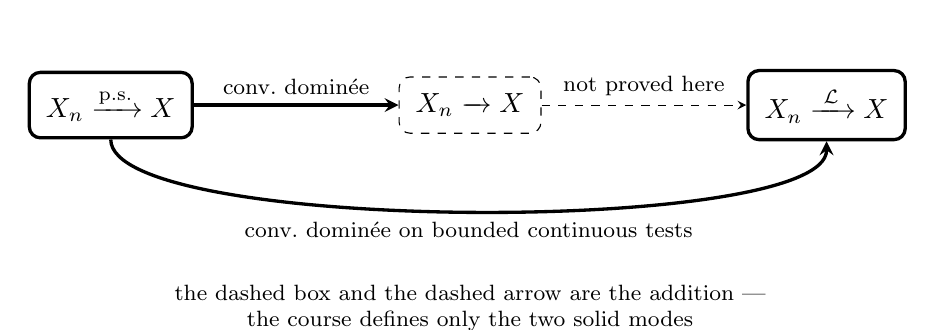
\begin{tikzpicture}[>=stealth, node distance=12mm and 26mm]
    \node[draw, very thick, rounded corners, inner sep=6pt] (as)
      {$X_{n} \cvas X$};
    \node[draw, dashed, rounded corners, inner sep=6pt, right=of as] (p)
      {$X_{n} \cvP X$};
    \node[draw, very thick, rounded corners, inner sep=6pt, right=of p] (l)
      {$X_{n} \cvL X$};
    \draw[->, very thick] (as) -- node[above,font=\footnotesize] {conv.\ dominée} (p);
    \draw[->, dashed] (p) -- node[above,font=\footnotesize] {not proved here} (l);
    \draw[->, very thick] (as.south) .. controls +(0,-1.2) and +(0,-1.2) ..
      node[below,font=\footnotesize]
      {conv.\ dominée on bounded continuous tests} (l.south);
    \node[below=18mm of p, align=center, font=\footnotesize]
      {the dashed box and the dashed arrow are the addition ---\\
       the course defines only the two solid modes};
  \end{tikzpicture}
\end{figure}

\begin{remark}[No arrow reverses]
  Convergence presque sûre implies convergence en probabilité --- proved in
  chapter 8 --- and convergence en probabilité implies convergence en loi,
  an implication carried here without proof; neither converse holds. An indicator
  window of width $1/n$ sliding cyclically around $[0,1]$ has $\prob(|X_{n}| > a)
  = 1/n \to 0$, so $X_{n} \cvP 0$, while every $\omega$ is hit infinitely often
  and $X_{n}(\omega)$
  converges for no $\omega$ at all. And with $X$ of loi normale centrée réduite and
  $X_{n} = -X$ for every $n$, the lois are equal so $X_{n} \cvL X$ holds trivially,
  while $|X_{n} - X| = 2|X|$ never gets small. The one partial converse worth
  knowing belongs to the addition and is stated, not proved, in these notes:
  convergence en loi \emph{to a constant} does imply convergence en probabilité to
  that constant.
\end{remark}

The practical criterion for convergence en loi is not the definition but the
fonction caractéristique, and it comes from two results used together. Chapter 6
proves that the fonction caractéristique determines the loi:
$\prob_{X} = \prob_{Y}$ if and only if $\varphi_{X} = \varphi_{Y}$. Chapter 8's
theorem on the three characterisations of convergence en loi then upgrades that
from lois to sequences of lois.

\begin{theorem}[Trois caractérisations de la convergence en loi]
  Soit $X_{1}, X_{2}, \dots$ une suite de variables aléatoires réelles, de
  fonctions caractéristiques respectives $\varphi_{1}, \varphi_{2}, \dots$, et
  $X$ une variable aléatoire réelle, de fonction caractéristique $\varphi$. Les
  propositions suivantes sont équivalentes :
  \begin{enumerate}
    \item $X_{n} \cvL X$ ;
    \item $\expec(\phi(X_{n})) \to \expec(\phi(X))$ pour toute fonction
      \emph{continue bornée} $\phi$ ;
    \item $\varphi_{n}(t) \to \varphi(t)$ pour tout $t \in \reals$.
  \end{enumerate}
\end{theorem}

The third characterisation is the one that gets used: to prove a convergence en
loi, compute the fonction caractéristique of the $n$-th term, take its
pointwise limit, and recognise the result. That is exactly how the théorème
central limite is proved.\\
Two hypotheses inside the criterion are worth keeping in view. The fonctions test
of the second characterisation must be bounded \emph{and} continuous ---
boundedness alone is what makes convergence dominée available, and continuity
alone is what lets convergence presque sûre be pushed through. And the pointwise
convergence of the third is convergence at every real $t$, not on a neighbourhood
of $0$ and not uniformly.\\
Which mode does each theorem deliver? The two results of chapter 8 answer
differently, and confusing them is the standard error.

\begin{theorem}[Loi forte des grands nombres]
  Pour toute suite $X_{1}, X_{2}, \dots$ de variables aléatoires réelles
  i.i.d.\ \emph{ayant une espérance},
  \[
    \frac{1}{n}\sum_{i=1}^{n} X_{i} \cvas \expec(X_{1}).
  \]
\end{theorem}

\begin{theorem}[Théorème central limite]
  Pour toute suite $X_{1}, X_{2}, \dots$ de variables aléatoires réelles
  i.i.d.\ d'espérance finie $\mu$ et de variance finie $\sigma^{2}$,
  \[
    \sqrt{n}\left(\frac{1}{n}\sum_{i=1}^{n} X_{i} - \mu\right)
      \cvL \mathcal{N}(0,\sigma^{2}).
  \]
\end{theorem}

\begin{remark}[The hypotheses are not interchangeable either]
  The loi forte asks for an espérance, that is $\expec(|X_{1}|) < +\infty$, and
  \emph{not} for a finite variance; the finite variance belongs to the weak law and
  to one proof of the loi forte, and importing it into the statement weakens the
  theorem for nothing. The théorème central limite does need a finite variance,
  since $\sigma^{2}$ appears in its conclusion. So the loi forte delivers the
  strongest mode under the weaker hypothesis, and the théorème central limite the
  weakest mode under the stronger one --- which is not a paradox: they say
  different things, one about where the mean goes and one about how large the
  error is on the way.
\end{remark}

\begin{conclusion}
Five symbols in these notes carry more than one meaning, because the course's
notation is kept as exams use it, collisions included, and each time the meaning is fixed by what
sits in the parentheses. $\mathcal{P}$ is the ensemble des parties
$\mathcal{P}(\Omega)$ and the loi de Poisson $\mathcal{P}(\lambda)$. $\mathcal{B}$
is the tribu de Borel $\mathcal{B}(\reals)$, the loi de Bernoulli
$\mathcal{B}(p)$, the loi binomiale $\mathcal{B}(n,p)$ and the loi Beta
$\mathcal{B}(a,b)$. $\lambda$ is the mesure de Lebesgue and the parameter of the
loi exponentielle and the loi de Poisson. $\Gamma$ is the loi Gamma
$\Gamma(a,\lambda)$ and the matrice de covariance of a vecteur gaussien,
$\mathcal{N}(\mu,\Gamma)$ --- and, in the densité of the loi Gamma, also the gamma
function. $\mathcal{E}$ is a generic tribu, as in $(E,\mathcal{E})$, and the loi
exponentielle $\mathcal{E}(\lambda)$. All five appear in the tables above in their
meaning as a loi, and two of them collide there on a single page: $\mathcal{B}$
carries the loi de Bernoulli, the loi binomiale and the loi Beta in the same two
tables, and the Gamma row prints the loi Gamma and the gamma function
side by side. That is why the notation column is the one to read first.
\end{conclusion}


\end{document}
